\documentclass[twoside]{book}

% Packages required by doxygen
\usepackage{fixltx2e}
\usepackage{calc}
\usepackage{doxygen}
\usepackage[export]{adjustbox} % also loads graphicx
\usepackage{graphicx}
\usepackage[utf8]{inputenc}
\usepackage{makeidx}
\usepackage{multicol}
\usepackage{multirow}
\PassOptionsToPackage{warn}{textcomp}
\usepackage{textcomp}
\usepackage[nointegrals]{wasysym}
\usepackage[table]{xcolor}

% Font selection
\usepackage[T1]{fontenc}
\usepackage[scaled=.90]{helvet}
\usepackage{courier}
\usepackage{amssymb}
\usepackage{sectsty}
\renewcommand{\familydefault}{\sfdefault}
\allsectionsfont{%
  \fontseries{bc}\selectfont%
  \color{darkgray}%
}
\renewcommand{\DoxyLabelFont}{%
  \fontseries{bc}\selectfont%
  \color{darkgray}%
}
\newcommand{\+}{\discretionary{\mbox{\scriptsize$\hookleftarrow$}}{}{}}

% Page & text layout
\usepackage{geometry}
\geometry{%
  a4paper,%
  top=2.5cm,%
  bottom=2.5cm,%
  left=2.5cm,%
  right=2.5cm%
}
\tolerance=750
\hfuzz=15pt
\hbadness=750
\setlength{\emergencystretch}{15pt}
\setlength{\parindent}{0cm}
\setlength{\parskip}{3ex plus 2ex minus 2ex}
\makeatletter
\renewcommand{\paragraph}{%
  \@startsection{paragraph}{4}{0ex}{-1.0ex}{1.0ex}{%
    \normalfont\normalsize\bfseries\SS@parafont%
  }%
}
\renewcommand{\subparagraph}{%
  \@startsection{subparagraph}{5}{0ex}{-1.0ex}{1.0ex}{%
    \normalfont\normalsize\bfseries\SS@subparafont%
  }%
}
\makeatother

% Headers & footers
\usepackage{fancyhdr}
\pagestyle{fancyplain}
\fancyhead[LE]{\fancyplain{}{\bfseries\thepage}}
\fancyhead[CE]{\fancyplain{}{}}
\fancyhead[RE]{\fancyplain{}{\bfseries\leftmark}}
\fancyhead[LO]{\fancyplain{}{\bfseries\rightmark}}
\fancyhead[CO]{\fancyplain{}{}}
\fancyhead[RO]{\fancyplain{}{\bfseries\thepage}}
\fancyfoot[LE]{\fancyplain{}{}}
\fancyfoot[CE]{\fancyplain{}{}}
\fancyfoot[RE]{\fancyplain{}{\bfseries\scriptsize Generated by Doxygen }}
\fancyfoot[LO]{\fancyplain{}{\bfseries\scriptsize Generated by Doxygen }}
\fancyfoot[CO]{\fancyplain{}{}}
\fancyfoot[RO]{\fancyplain{}{}}
\renewcommand{\footrulewidth}{0.4pt}
\renewcommand{\chaptermark}[1]{%
  \markboth{#1}{}%
}
\renewcommand{\sectionmark}[1]{%
  \markright{\thesection\ #1}%
}

% Indices & bibliography
\usepackage{natbib}
\usepackage[titles]{tocloft}
\setcounter{tocdepth}{3}
\setcounter{secnumdepth}{5}
\makeindex

% Hyperlinks (required, but should be loaded last)
\usepackage{ifpdf}
\ifpdf
  \usepackage[pdftex,pagebackref=true]{hyperref}
\else
  \usepackage[ps2pdf,pagebackref=true]{hyperref}
\fi
\hypersetup{%
  colorlinks=true,%
  linkcolor=blue,%
  citecolor=blue,%
  unicode%
}

% Custom commands
\newcommand{\clearemptydoublepage}{%
  \newpage{\pagestyle{empty}\cleardoublepage}%
}

\usepackage{caption}
\captionsetup{labelsep=space,justification=centering,font={bf},singlelinecheck=off,skip=4pt,position=top}

%===== C O N T E N T S =====

\begin{document}

% Titlepage & ToC
\hypersetup{pageanchor=false,
             bookmarksnumbered=true,
             pdfencoding=unicode
            }
\pagenumbering{alph}
\begin{titlepage}
\vspace*{7cm}
\begin{center}%
{\Large Perceus }\\
\vspace*{1cm}
{\large Generated by Doxygen 1.8.13}\\
\end{center}
\end{titlepage}
\clearemptydoublepage
\pagenumbering{roman}
\tableofcontents
\clearemptydoublepage
\pagenumbering{arabic}
\hypersetup{pageanchor=true}

%--- Begin generated contents ---
\chapter{Namespace Index}
\section{Namespace List}
Here is a list of all namespaces with brief descriptions\+:\begin{DoxyCompactList}
\item\contentsline{section}{\hyperlink{namespacepcs}{pcs} }{\pageref{namespacepcs}}{}
\item\contentsline{section}{\hyperlink{namespacepcs_1_1Data}{pcs\+::\+Data} }{\pageref{namespacepcs_1_1Data}}{}
\item\contentsline{section}{\hyperlink{namespacepcs_1_1rend}{pcs\+::rend} }{\pageref{namespacepcs_1_1rend}}{}
\item\contentsline{section}{\hyperlink{namespacepcs_1_1Util}{pcs\+::\+Util} }{\pageref{namespacepcs_1_1Util}}{}
\item\contentsline{section}{\hyperlink{namespacepcs_1_1Util_1_1Mem}{pcs\+::\+Util\+::\+Mem} }{\pageref{namespacepcs_1_1Util_1_1Mem}}{}
\end{DoxyCompactList}

\chapter{Hierarchical Index}
\section{Class Hierarchy}
This inheritance list is sorted roughly, but not completely, alphabetically\+:\begin{DoxyCompactList}
\item \contentsline{section}{pcs\+:\+:Util\+:\+:Linked\+List$<$ T $>$\+:\+:\+\_\+\+Point}{\pageref{structpcs_1_1Util_1_1LinkedList_1_1__Point}}{}
\item \contentsline{section}{pcs\+:\+:Color}{\pageref{structpcs_1_1Color}}{}
\item \contentsline{section}{pcs\+:\+:Util\+:\+:Mem\+:\+:Data\+Point}{\pageref{structpcs_1_1Util_1_1Mem_1_1DataPoint}}{}
\item \contentsline{section}{pcs\+:\+:Event}{\pageref{classpcs_1_1Event}}{}
\begin{DoxyCompactList}
\item \contentsline{section}{pcs\+:\+:Key\+Event}{\pageref{classpcs_1_1KeyEvent}}{}
\begin{DoxyCompactList}
\item \contentsline{section}{pcs\+:\+:Key\+Down\+Event}{\pageref{classpcs_1_1KeyDownEvent}}{}
\item \contentsline{section}{pcs\+:\+:Key\+Press\+Event}{\pageref{classpcs_1_1KeyPressEvent}}{}
\item \contentsline{section}{pcs\+:\+:Key\+Release\+Event}{\pageref{classpcs_1_1KeyReleaseEvent}}{}
\end{DoxyCompactList}
\item \contentsline{section}{pcs\+:\+:Window\+Closed\+Event}{\pageref{classpcs_1_1WindowClosedEvent}}{}
\end{DoxyCompactList}
\item \contentsline{section}{pcs\+:\+:File}{\pageref{classpcs_1_1File}}{}
\begin{DoxyCompactList}
\item \contentsline{section}{pcs\+:\+:Util\+:\+:Raw\+Model\+Parser}{\pageref{classpcs_1_1Util_1_1RawModelParser}}{}
\begin{DoxyCompactList}
\item \contentsline{section}{pcs\+:\+:Parser\+O\+BJ}{\pageref{classpcs_1_1ParserOBJ}}{}
\end{DoxyCompactList}
\end{DoxyCompactList}
\item \contentsline{section}{pcs\+:\+:Util\+:\+:Linked\+List$<$ T $>$}{\pageref{classpcs_1_1Util_1_1LinkedList}}{}
\item \contentsline{section}{pcs\+:\+:Log}{\pageref{classpcs_1_1Log}}{}
\item \contentsline{section}{pcs\+:\+:Mat4f}{\pageref{structpcs_1_1Mat4f}}{}
\item \contentsline{section}{pcs\+:\+:Data\+:\+:Non\+Copyable}{\pageref{structpcs_1_1Data_1_1NonCopyable}}{}
\begin{DoxyCompactList}
\item \contentsline{section}{pcs\+:\+:rend\+:\+:Render\+Surface$<$ T $>$}{\pageref{classpcs_1_1rend_1_1RenderSurface}}{}
\item \contentsline{section}{pcs\+:\+:rend\+:\+:Render\+Surface$<$ unsigned int $>$}{\pageref{classpcs_1_1rend_1_1RenderSurface}}{}
\begin{DoxyCompactList}
\item \contentsline{section}{pcs\+:\+:Window}{\pageref{classpcs_1_1Window}}{}
\end{DoxyCompactList}
\end{DoxyCompactList}
\item \contentsline{section}{pcs\+:\+:Data\+:\+:Object\+ID$<$ T, R $>$}{\pageref{classpcs_1_1Data_1_1ObjectID}}{}
\item \contentsline{section}{pcs\+:\+:Data\+:\+:Object\+ID$<$ Buffer $>$}{\pageref{classpcs_1_1Data_1_1ObjectID}}{}
\begin{DoxyCompactList}
\item \contentsline{section}{pcs\+:\+:rend\+:\+:Buffer}{\pageref{classpcs_1_1rend_1_1Buffer}}{}
\end{DoxyCompactList}
\item \contentsline{section}{pcs\+:\+:Data\+:\+:Object\+ID$<$ Buffer\+Array $>$}{\pageref{classpcs_1_1Data_1_1ObjectID}}{}
\begin{DoxyCompactList}
\item \contentsline{section}{pcs\+:\+:rend\+:\+:Buffer\+Array}{\pageref{classpcs_1_1rend_1_1BufferArray}}{}
\begin{DoxyCompactList}
\item \contentsline{section}{pcs\+:\+:Raw\+Model}{\pageref{classpcs_1_1RawModel}}{}
\end{DoxyCompactList}
\end{DoxyCompactList}
\item \contentsline{section}{pcs\+:\+:Data\+:\+:Object\+ID$<$ Object\+U\+ID, U64 $>$}{\pageref{classpcs_1_1Data_1_1ObjectID}}{}
\begin{DoxyCompactList}
\item \contentsline{section}{pcs\+:\+:Data\+:\+:Object\+U\+ID}{\pageref{classpcs_1_1Data_1_1ObjectUID}}{}
\begin{DoxyCompactList}
\item \contentsline{section}{pcs\+:\+:Camera}{\pageref{classpcs_1_1Camera}}{}
\item \contentsline{section}{pcs\+:\+:Window}{\pageref{classpcs_1_1Window}}{}
\end{DoxyCompactList}
\end{DoxyCompactList}
\item \contentsline{section}{pcs\+:\+:Data\+:\+:Object\+ID$<$ Shader $>$}{\pageref{classpcs_1_1Data_1_1ObjectID}}{}
\begin{DoxyCompactList}
\item \contentsline{section}{pcs\+:\+:Shader}{\pageref{classpcs_1_1Shader}}{}
\end{DoxyCompactList}
\item \contentsline{section}{pcs\+:\+:Data\+:\+:Object\+ID$<$ Shader\+Program $>$}{\pageref{classpcs_1_1Data_1_1ObjectID}}{}
\begin{DoxyCompactList}
\item \contentsline{section}{pcs\+:\+:Shader\+Program}{\pageref{classpcs_1_1ShaderProgram}}{}
\end{DoxyCompactList}
\item \contentsline{section}{pcs\+:\+:Data\+:\+:Object\+ID$<$ Texture $>$}{\pageref{classpcs_1_1Data_1_1ObjectID}}{}
\begin{DoxyCompactList}
\item \contentsline{section}{pcs\+:\+:Texture}{\pageref{classpcs_1_1Texture}}{}
\end{DoxyCompactList}
\item \contentsline{section}{pcs\+:\+:rend\+:\+:Render\+A\+PI}{\pageref{structpcs_1_1rend_1_1RenderAPI}}{}
\item \contentsline{section}{pcs\+:\+:rend\+:\+:Render\+Object}{\pageref{classpcs_1_1rend_1_1RenderObject}}{}
\begin{DoxyCompactList}
\item \contentsline{section}{pcs\+:\+:Engine}{\pageref{classpcs_1_1Engine}}{}
\item \contentsline{section}{pcs\+:\+:rend\+:\+:Buffer}{\pageref{classpcs_1_1rend_1_1Buffer}}{}
\item \contentsline{section}{pcs\+:\+:rend\+:\+:Buffer\+Array}{\pageref{classpcs_1_1rend_1_1BufferArray}}{}
\item \contentsline{section}{pcs\+:\+:rend\+:\+:Render\+Surface$<$ T $>$}{\pageref{classpcs_1_1rend_1_1RenderSurface}}{}
\item \contentsline{section}{pcs\+:\+:Renderer}{\pageref{classpcs_1_1Renderer}}{}
\begin{DoxyCompactList}
\item \contentsline{section}{pcs\+:\+:Forward\+Renderer}{\pageref{classpcs_1_1ForwardRenderer}}{}
\end{DoxyCompactList}
\item \contentsline{section}{pcs\+:\+:Scene}{\pageref{classpcs_1_1Scene}}{}
\item \contentsline{section}{pcs\+:\+:Shader}{\pageref{classpcs_1_1Shader}}{}
\item \contentsline{section}{pcs\+:\+:Shader\+Program}{\pageref{classpcs_1_1ShaderProgram}}{}
\item \contentsline{section}{pcs\+:\+:Texture}{\pageref{classpcs_1_1Texture}}{}
\item \contentsline{section}{pcs\+:\+:rend\+:\+:Render\+Surface$<$ unsigned int $>$}{\pageref{classpcs_1_1rend_1_1RenderSurface}}{}
\end{DoxyCompactList}
\item \contentsline{section}{pcs\+:\+:rend\+:\+:Render\+Settings}{\pageref{structpcs_1_1rend_1_1RenderSettings}}{}
\item \contentsline{section}{pcs\+:\+:Data\+:\+:Singleton$<$ T $>$}{\pageref{classpcs_1_1Data_1_1Singleton}}{}
\item \contentsline{section}{pcs\+:\+:Data\+:\+:Singleton$<$ Engine $>$}{\pageref{classpcs_1_1Data_1_1Singleton}}{}
\begin{DoxyCompactList}
\item \contentsline{section}{pcs\+:\+:Engine}{\pageref{classpcs_1_1Engine}}{}
\end{DoxyCompactList}
\item \contentsline{section}{pcs\+:\+:Data\+:\+:Singleton$<$ Event\+Handler $>$}{\pageref{classpcs_1_1Data_1_1Singleton}}{}
\begin{DoxyCompactList}
\item \contentsline{section}{pcs\+:\+:Event\+Handler}{\pageref{classpcs_1_1EventHandler}}{}
\end{DoxyCompactList}
\item \contentsline{section}{pcs\+:\+:Data\+:\+:Singleton$<$ Forward\+Renderer $>$}{\pageref{classpcs_1_1Data_1_1Singleton}}{}
\begin{DoxyCompactList}
\item \contentsline{section}{pcs\+:\+:Forward\+Renderer}{\pageref{classpcs_1_1ForwardRenderer}}{}
\end{DoxyCompactList}
\item \contentsline{section}{pcs\+:\+:Data\+:\+:Singleton$<$ Reg\+Table $>$}{\pageref{classpcs_1_1Data_1_1Singleton}}{}
\begin{DoxyCompactList}
\item \contentsline{section}{pcs\+:\+:Util\+:\+:Mem\+:\+:Reg\+Table}{\pageref{classpcs_1_1Util_1_1Mem_1_1RegTable}}{}
\end{DoxyCompactList}
\item \contentsline{section}{pcs\+:\+:Sizable$<$ T $>$}{\pageref{structpcs_1_1Sizable}}{}
\begin{DoxyCompactList}
\item \contentsline{section}{pcs\+:\+:rend\+:\+:Render\+Surface$<$ T $>$}{\pageref{classpcs_1_1rend_1_1RenderSurface}}{}
\end{DoxyCompactList}
\item \contentsline{section}{pcs\+:\+:Sizable$<$ unsigned int $>$}{\pageref{structpcs_1_1Sizable}}{}
\begin{DoxyCompactList}
\item \contentsline{section}{pcs\+:\+:rend\+:\+:Render\+Surface$<$ unsigned int $>$}{\pageref{classpcs_1_1rend_1_1RenderSurface}}{}
\end{DoxyCompactList}
\item \contentsline{section}{pcs\+:\+:Stack$<$ T $>$}{\pageref{classpcs_1_1Stack}}{}
\item \contentsline{section}{pcs\+:\+:Data\+:\+:Status$<$ E $>$}{\pageref{classpcs_1_1Data_1_1Status}}{}
\item \contentsline{section}{pcs\+:\+:Data\+:\+:Status$<$ Exit\+Code $>$}{\pageref{classpcs_1_1Data_1_1Status}}{}
\begin{DoxyCompactList}
\item \contentsline{section}{pcs\+:\+:Application}{\pageref{classpcs_1_1Application}}{}
\end{DoxyCompactList}
\item \contentsline{section}{pcs\+:\+:Data\+:\+:Status$<$ Render\+Status $>$}{\pageref{classpcs_1_1Data_1_1Status}}{}
\begin{DoxyCompactList}
\item \contentsline{section}{pcs\+:\+:Engine}{\pageref{classpcs_1_1Engine}}{}
\end{DoxyCompactList}
\item \contentsline{section}{pcs\+:\+:Data\+:\+:Status$<$ Scene\+State $>$}{\pageref{classpcs_1_1Data_1_1Status}}{}
\begin{DoxyCompactList}
\item \contentsline{section}{pcs\+:\+:Scene}{\pageref{classpcs_1_1Scene}}{}
\end{DoxyCompactList}
\item \contentsline{section}{pcs\+:\+:Data\+:\+:Status$<$ Shader\+Status $>$}{\pageref{classpcs_1_1Data_1_1Status}}{}
\begin{DoxyCompactList}
\item \contentsline{section}{pcs\+:\+:Shader}{\pageref{classpcs_1_1Shader}}{}
\end{DoxyCompactList}
\item \contentsline{section}{pcs\+:\+:Data\+:\+:Status$<$ Window\+Status $>$}{\pageref{classpcs_1_1Data_1_1Status}}{}
\begin{DoxyCompactList}
\item \contentsline{section}{pcs\+:\+:Window}{\pageref{classpcs_1_1Window}}{}
\end{DoxyCompactList}
\item \contentsline{section}{pcs\+:\+:Texture\+Array}{\pageref{unionpcs_1_1TextureArray}}{}
\item \contentsline{section}{pcs\+:\+:Transformable$<$ T $>$}{\pageref{classpcs_1_1Transformable}}{}
\item \contentsline{section}{pcs\+:\+:Transformable$<$ Vec2$<$ T $>$ $>$}{\pageref{classpcs_1_1Transformable}}{}
\begin{DoxyCompactList}
\item \contentsline{section}{pcs\+:\+:Transformable2D$<$ T $>$}{\pageref{classpcs_1_1Transformable2D}}{}
\end{DoxyCompactList}
\item \contentsline{section}{pcs\+:\+:Transformable$<$ Vec3$<$ float $>$ $>$}{\pageref{classpcs_1_1Transformable}}{}
\begin{DoxyCompactList}
\item \contentsline{section}{pcs\+:\+:Transformable3D$<$ float $>$}{\pageref{classpcs_1_1Transformable3D}}{}
\begin{DoxyCompactList}
\item \contentsline{section}{pcs\+:\+:Camera}{\pageref{classpcs_1_1Camera}}{}
\item \contentsline{section}{pcs\+:\+:Model}{\pageref{classpcs_1_1Model}}{}
\end{DoxyCompactList}
\end{DoxyCompactList}
\item \contentsline{section}{pcs\+:\+:Transformable$<$ Vec3$<$ T $>$ $>$}{\pageref{classpcs_1_1Transformable}}{}
\begin{DoxyCompactList}
\item \contentsline{section}{pcs\+:\+:Transformable3D$<$ T $>$}{\pageref{classpcs_1_1Transformable3D}}{}
\end{DoxyCompactList}
\item \contentsline{section}{pcs\+:\+:Vec2$<$ T $>$}{\pageref{structpcs_1_1Vec2}}{}
\item \contentsline{section}{pcs\+:\+:Vec2$<$ float $>$}{\pageref{structpcs_1_1Vec2}}{}
\item \contentsline{section}{pcs\+:\+:Vec2$<$ unsigned int $>$}{\pageref{structpcs_1_1Vec2}}{}
\item \contentsline{section}{pcs\+:\+:Vec3$<$ T $>$}{\pageref{structpcs_1_1Vec3}}{}
\item \contentsline{section}{pcs\+:\+:Vec3$<$ float $>$}{\pageref{structpcs_1_1Vec3}}{}
\item \contentsline{section}{pcs\+:\+:Vec4$<$ T $>$}{\pageref{structpcs_1_1Vec4}}{}
\item \contentsline{section}{pcs\+:\+:Vertex}{\pageref{structpcs_1_1Vertex}}{}
\item \contentsline{section}{pcs\+:\+:Vertex\+Array}{\pageref{classpcs_1_1VertexArray}}{}
\end{DoxyCompactList}

\chapter{Class Index}
\section{Class List}
Here are the classes, structs, unions and interfaces with brief descriptions\+:\begin{DoxyCompactList}
\item\contentsline{section}{\hyperlink{structpcs_1_1Util_1_1LinkedList_1_1__Point}{pcs\+::\+Util\+::\+Linked\+List$<$ T $>$\+::\+\_\+\+Point} }{\pageref{structpcs_1_1Util_1_1LinkedList_1_1__Point}}{}
\item\contentsline{section}{\hyperlink{classpcs_1_1Application}{pcs\+::\+Application} \\*Handles and runs the entire engine process. This is where the main loop is, this holds the engine }{\pageref{classpcs_1_1Application}}{}
\item\contentsline{section}{\hyperlink{classpcs_1_1rend_1_1Buffer}{pcs\+::rend\+::\+Buffer} }{\pageref{classpcs_1_1rend_1_1Buffer}}{}
\item\contentsline{section}{\hyperlink{classpcs_1_1rend_1_1BufferArray}{pcs\+::rend\+::\+Buffer\+Array} }{\pageref{classpcs_1_1rend_1_1BufferArray}}{}
\item\contentsline{section}{\hyperlink{classpcs_1_1Camera}{pcs\+::\+Camera} }{\pageref{classpcs_1_1Camera}}{}
\item\contentsline{section}{\hyperlink{structpcs_1_1Color}{pcs\+::\+Color} }{\pageref{structpcs_1_1Color}}{}
\item\contentsline{section}{\hyperlink{structpcs_1_1Util_1_1Mem_1_1DataPoint}{pcs\+::\+Util\+::\+Mem\+::\+Data\+Point} }{\pageref{structpcs_1_1Util_1_1Mem_1_1DataPoint}}{}
\item\contentsline{section}{\hyperlink{classpcs_1_1Engine}{pcs\+::\+Engine} \\*Handles rendering and holds the window instance }{\pageref{classpcs_1_1Engine}}{}
\item\contentsline{section}{\hyperlink{classpcs_1_1Event}{pcs\+::\+Event} }{\pageref{classpcs_1_1Event}}{}
\item\contentsline{section}{\hyperlink{classpcs_1_1EventHandler}{pcs\+::\+Event\+Handler} }{\pageref{classpcs_1_1EventHandler}}{}
\item\contentsline{section}{\hyperlink{classpcs_1_1File}{pcs\+::\+File} }{\pageref{classpcs_1_1File}}{}
\item\contentsline{section}{\hyperlink{classpcs_1_1ForwardRenderer}{pcs\+::\+Forward\+Renderer} }{\pageref{classpcs_1_1ForwardRenderer}}{}
\item\contentsline{section}{\hyperlink{classpcs_1_1KeyDownEvent}{pcs\+::\+Key\+Down\+Event} }{\pageref{classpcs_1_1KeyDownEvent}}{}
\item\contentsline{section}{\hyperlink{classpcs_1_1KeyEvent}{pcs\+::\+Key\+Event} }{\pageref{classpcs_1_1KeyEvent}}{}
\item\contentsline{section}{\hyperlink{classpcs_1_1KeyPressEvent}{pcs\+::\+Key\+Press\+Event} }{\pageref{classpcs_1_1KeyPressEvent}}{}
\item\contentsline{section}{\hyperlink{classpcs_1_1KeyReleaseEvent}{pcs\+::\+Key\+Release\+Event} }{\pageref{classpcs_1_1KeyReleaseEvent}}{}
\item\contentsline{section}{\hyperlink{classpcs_1_1Util_1_1LinkedList}{pcs\+::\+Util\+::\+Linked\+List$<$ T $>$} }{\pageref{classpcs_1_1Util_1_1LinkedList}}{}
\item\contentsline{section}{\hyperlink{classpcs_1_1Log}{pcs\+::\+Log} }{\pageref{classpcs_1_1Log}}{}
\item\contentsline{section}{\hyperlink{structpcs_1_1Mat4f}{pcs\+::\+Mat4f} }{\pageref{structpcs_1_1Mat4f}}{}
\item\contentsline{section}{\hyperlink{classpcs_1_1Model}{pcs\+::\+Model} }{\pageref{classpcs_1_1Model}}{}
\item\contentsline{section}{\hyperlink{structpcs_1_1Data_1_1NonCopyable}{pcs\+::\+Data\+::\+Non\+Copyable} }{\pageref{structpcs_1_1Data_1_1NonCopyable}}{}
\item\contentsline{section}{\hyperlink{classpcs_1_1Data_1_1ObjectID}{pcs\+::\+Data\+::\+Object\+I\+D$<$ T, R $>$} \\*Class that handles an object\textquotesingle{}s unique ID }{\pageref{classpcs_1_1Data_1_1ObjectID}}{}
\item\contentsline{section}{\hyperlink{classpcs_1_1Data_1_1ObjectUID}{pcs\+::\+Data\+::\+Object\+U\+ID} }{\pageref{classpcs_1_1Data_1_1ObjectUID}}{}
\item\contentsline{section}{\hyperlink{classpcs_1_1ParserOBJ}{pcs\+::\+Parser\+O\+BJ} }{\pageref{classpcs_1_1ParserOBJ}}{}
\item\contentsline{section}{\hyperlink{classpcs_1_1RawModel}{pcs\+::\+Raw\+Model} }{\pageref{classpcs_1_1RawModel}}{}
\item\contentsline{section}{\hyperlink{classpcs_1_1Util_1_1RawModelParser}{pcs\+::\+Util\+::\+Raw\+Model\+Parser} }{\pageref{classpcs_1_1Util_1_1RawModelParser}}{}
\item\contentsline{section}{\hyperlink{classpcs_1_1Util_1_1Mem_1_1RegTable}{pcs\+::\+Util\+::\+Mem\+::\+Reg\+Table} }{\pageref{classpcs_1_1Util_1_1Mem_1_1RegTable}}{}
\item\contentsline{section}{\hyperlink{structpcs_1_1rend_1_1RenderAPI}{pcs\+::rend\+::\+Render\+A\+PI} }{\pageref{structpcs_1_1rend_1_1RenderAPI}}{}
\item\contentsline{section}{\hyperlink{classpcs_1_1Renderer}{pcs\+::\+Renderer} }{\pageref{classpcs_1_1Renderer}}{}
\item\contentsline{section}{\hyperlink{classpcs_1_1rend_1_1RenderObject}{pcs\+::rend\+::\+Render\+Object} \\*Class for retreiving the currently selected render A\+PI }{\pageref{classpcs_1_1rend_1_1RenderObject}}{}
\item\contentsline{section}{\hyperlink{structpcs_1_1rend_1_1RenderSettings}{pcs\+::rend\+::\+Render\+Settings} \\*Container for choosing various A\+PI types }{\pageref{structpcs_1_1rend_1_1RenderSettings}}{}
\item\contentsline{section}{\hyperlink{classpcs_1_1rend_1_1RenderSurface}{pcs\+::rend\+::\+Render\+Surface$<$ T $>$} \\*Class that handles basic rendering functionality }{\pageref{classpcs_1_1rend_1_1RenderSurface}}{}
\item\contentsline{section}{\hyperlink{classpcs_1_1Scene}{pcs\+::\+Scene} }{\pageref{classpcs_1_1Scene}}{}
\item\contentsline{section}{\hyperlink{classpcs_1_1Shader}{pcs\+::\+Shader} }{\pageref{classpcs_1_1Shader}}{}
\item\contentsline{section}{\hyperlink{classpcs_1_1ShaderProgram}{pcs\+::\+Shader\+Program} }{\pageref{classpcs_1_1ShaderProgram}}{}
\item\contentsline{section}{\hyperlink{classpcs_1_1Data_1_1Singleton}{pcs\+::\+Data\+::\+Singleton$<$ T $>$} }{\pageref{classpcs_1_1Data_1_1Singleton}}{}
\item\contentsline{section}{\hyperlink{structpcs_1_1Sizable}{pcs\+::\+Sizable$<$ T $>$} }{\pageref{structpcs_1_1Sizable}}{}
\item\contentsline{section}{\hyperlink{classpcs_1_1Stack}{pcs\+::\+Stack$<$ T $>$} }{\pageref{classpcs_1_1Stack}}{}
\item\contentsline{section}{\hyperlink{classpcs_1_1Data_1_1Status}{pcs\+::\+Data\+::\+Status$<$ E $>$} }{\pageref{classpcs_1_1Data_1_1Status}}{}
\item\contentsline{section}{\hyperlink{classpcs_1_1Texture}{pcs\+::\+Texture} }{\pageref{classpcs_1_1Texture}}{}
\item\contentsline{section}{\hyperlink{unionpcs_1_1TextureArray}{pcs\+::\+Texture\+Array} }{\pageref{unionpcs_1_1TextureArray}}{}
\item\contentsline{section}{\hyperlink{classpcs_1_1Transformable}{pcs\+::\+Transformable$<$ T $>$} \\*Class that handles rotation, translation, and scale }{\pageref{classpcs_1_1Transformable}}{}
\item\contentsline{section}{\hyperlink{classpcs_1_1Transformable2D}{pcs\+::\+Transformable2\+D$<$ T $>$} \\*Class that handles 2-\/\+Dimensional Transformations }{\pageref{classpcs_1_1Transformable2D}}{}
\item\contentsline{section}{\hyperlink{classpcs_1_1Transformable3D}{pcs\+::\+Transformable3\+D$<$ T $>$} \\*Class that handles 3-\/\+Dimensional Transformations }{\pageref{classpcs_1_1Transformable3D}}{}
\item\contentsline{section}{\hyperlink{structpcs_1_1Vec2}{pcs\+::\+Vec2$<$ T $>$} }{\pageref{structpcs_1_1Vec2}}{}
\item\contentsline{section}{\hyperlink{structpcs_1_1Vec3}{pcs\+::\+Vec3$<$ T $>$} }{\pageref{structpcs_1_1Vec3}}{}
\item\contentsline{section}{\hyperlink{structpcs_1_1Vec4}{pcs\+::\+Vec4$<$ T $>$} }{\pageref{structpcs_1_1Vec4}}{}
\item\contentsline{section}{\hyperlink{structpcs_1_1Vertex}{pcs\+::\+Vertex} }{\pageref{structpcs_1_1Vertex}}{}
\item\contentsline{section}{\hyperlink{classpcs_1_1VertexArray}{pcs\+::\+Vertex\+Array} }{\pageref{classpcs_1_1VertexArray}}{}
\item\contentsline{section}{\hyperlink{classpcs_1_1Window}{pcs\+::\+Window} \\*Class that handles window functionality. Uses the specified Render\+A\+PI to construct a window as well as manipulate the size and location }{\pageref{classpcs_1_1Window}}{}
\item\contentsline{section}{\hyperlink{classpcs_1_1WindowClosedEvent}{pcs\+::\+Window\+Closed\+Event} }{\pageref{classpcs_1_1WindowClosedEvent}}{}
\end{DoxyCompactList}

\chapter{File Index}
\section{File List}
Here is a list of all files with brief descriptions\+:\begin{DoxyCompactList}
\item\contentsline{section}{include/\+Perceus/\hyperlink{Core_8h}{Core.\+h} }{\pageref{Core_8h}}{}
\item\contentsline{section}{include/\+Perceus/\+Core/\hyperlink{Application_8h}{Application.\+h} }{\pageref{Application_8h}}{}
\item\contentsline{section}{include/\+Perceus/\+Core/\hyperlink{Engine_8h}{Engine.\+h} }{\pageref{Engine_8h}}{}
\item\contentsline{section}{include/\+Perceus/\+Core/\hyperlink{EntryPoint_8h}{Entry\+Point.\+h} }{\pageref{EntryPoint_8h}}{}
\item\contentsline{section}{include/\+Perceus/\+Core/\hyperlink{Scene_8h}{Scene.\+h} }{\pageref{Scene_8h}}{}
\item\contentsline{section}{include/\+Perceus/\+Core/\+Graphics/\hyperlink{Texture_8h}{Texture.\+h} }{\pageref{Texture_8h}}{}
\item\contentsline{section}{include/\+Perceus/\+Core/\+Graphics/\hyperlink{Window_8h}{Window.\+h} }{\pageref{Window_8h}}{}
\item\contentsline{section}{include/\+Perceus/\+Core/\+Graphics/\+Entities/\hyperlink{Buffer_8h}{Buffer.\+h} }{\pageref{Buffer_8h}}{}
\item\contentsline{section}{include/\+Perceus/\+Core/\+Graphics/\+Entities/\hyperlink{BufferArray_8h}{Buffer\+Array.\+h} }{\pageref{BufferArray_8h}}{}
\item\contentsline{section}{include/\+Perceus/\+Core/\+Graphics/\+Entities/\hyperlink{Camera_8h}{Camera.\+h} }{\pageref{Camera_8h}}{}
\item\contentsline{section}{include/\+Perceus/\+Core/\+Graphics/\+Entities/\hyperlink{Model_8h}{Model.\+h} }{\pageref{Model_8h}}{}
\item\contentsline{section}{include/\+Perceus/\+Core/\+Graphics/\+Entities/\hyperlink{RawModel_8h}{Raw\+Model.\+h} }{\pageref{RawModel_8h}}{}
\item\contentsline{section}{include/\+Perceus/\+Core/\+Graphics/\+Entities/\hyperlink{VertexArray_8h}{Vertex\+Array.\+h} }{\pageref{VertexArray_8h}}{}
\item\contentsline{section}{include/\+Perceus/\+Core/\+Graphics/\+Rendering/\hyperlink{Events_8h}{Events.\+h} }{\pageref{Events_8h}}{}
\item\contentsline{section}{include/\+Perceus/\+Core/\+Graphics/\+Rendering/\hyperlink{ForwardRenderer_8h}{Forward\+Renderer.\+h} }{\pageref{ForwardRenderer_8h}}{}
\item\contentsline{section}{include/\+Perceus/\+Core/\+Graphics/\+Rendering/\hyperlink{OpenAPI_8h}{Open\+A\+P\+I.\+h} }{\pageref{OpenAPI_8h}}{}
\item\contentsline{section}{include/\+Perceus/\+Core/\+Graphics/\+Rendering/\hyperlink{RenderAPI_8h}{Render\+A\+P\+I.\+h} }{\pageref{RenderAPI_8h}}{}
\item\contentsline{section}{include/\+Perceus/\+Core/\+Graphics/\+Rendering/\hyperlink{Renderer_8h}{Renderer.\+h} }{\pageref{Renderer_8h}}{}
\item\contentsline{section}{include/\+Perceus/\+Core/\+Graphics/\+Rendering/\hyperlink{RenderObject_8h}{Render\+Object.\+h} }{\pageref{RenderObject_8h}}{}
\item\contentsline{section}{include/\+Perceus/\+Core/\+Graphics/\+Rendering/\hyperlink{RenderSurface_8h}{Render\+Surface.\+h} }{\pageref{RenderSurface_8h}}{}
\item\contentsline{section}{include/\+Perceus/\+Core/\+Graphics/\+Rendering/\+Events/\hyperlink{Event_8h}{Event.\+h} }{\pageref{Event_8h}}{}
\item\contentsline{section}{include/\+Perceus/\+Core/\+Graphics/\+Rendering/\+Events/\hyperlink{EventHandler_8h}{Event\+Handler.\+h} }{\pageref{EventHandler_8h}}{}
\item\contentsline{section}{include/\+Perceus/\+Core/\+Graphics/\+Rendering/\+Events/\hyperlink{KeyboardEvents_8h}{Keyboard\+Events.\+h} }{\pageref{KeyboardEvents_8h}}{}
\item\contentsline{section}{include/\+Perceus/\+Core/\+Graphics/\+Rendering/\+Events/\hyperlink{WindowEvents_8h}{Window\+Events.\+h} }{\pageref{WindowEvents_8h}}{}
\item\contentsline{section}{include/\+Perceus/\+Core/\+Graphics/\+Rendering/\+Shaders/\hyperlink{Shader_8h}{Shader.\+h} }{\pageref{Shader_8h}}{}
\item\contentsline{section}{include/\+Perceus/\+Core/\+Graphics/\+Rendering/\+Shaders/\hyperlink{ShaderProgram_8h}{Shader\+Program.\+h} }{\pageref{ShaderProgram_8h}}{}
\item\contentsline{section}{include/\+Perceus/\+Data/\hyperlink{Color_8h}{Color.\+h} }{\pageref{Color_8h}}{}
\item\contentsline{section}{include/\+Perceus/\+Data/\hyperlink{Inc_8h}{Inc.\+h} }{\pageref{Inc_8h}}{}
\item\contentsline{section}{include/\+Perceus/\+Data/\hyperlink{Matrix_8h}{Matrix.\+h} }{\pageref{Matrix_8h}}{}
\item\contentsline{section}{include/\+Perceus/\+Data/\hyperlink{NonCopyable_8h}{Non\+Copyable.\+h} }{\pageref{NonCopyable_8h}}{}
\item\contentsline{section}{include/\+Perceus/\+Data/\hyperlink{ObjectID_8h}{Object\+I\+D.\+h} }{\pageref{ObjectID_8h}}{}
\item\contentsline{section}{include/\+Perceus/\+Data/\hyperlink{Singleton_8h}{Singleton.\+h} }{\pageref{Singleton_8h}}{}
\item\contentsline{section}{include/\+Perceus/\+Data/\hyperlink{Sizable_8h}{Sizable.\+h} }{\pageref{Sizable_8h}}{}
\item\contentsline{section}{include/\+Perceus/\+Data/\hyperlink{Status_8h}{Status.\+h} }{\pageref{Status_8h}}{}
\item\contentsline{section}{include/\+Perceus/\+Data/\hyperlink{Transformable_8h}{Transformable.\+h} }{\pageref{Transformable_8h}}{}
\item\contentsline{section}{include/\+Perceus/\+Data/\hyperlink{Vector_8h}{Vector.\+h} }{\pageref{Vector_8h}}{}
\item\contentsline{section}{include/\+Perceus/\+Data/\hyperlink{Vertex_8h}{Vertex.\+h} }{\pageref{Vertex_8h}}{}
\item\contentsline{section}{include/\+Perceus/\+Util/\hyperlink{File_8h}{File.\+h} }{\pageref{File_8h}}{}
\item\contentsline{section}{include/\+Perceus/\+Util/\hyperlink{Log_8h}{Log.\+h} }{\pageref{Log_8h}}{}
\item\contentsline{section}{include/\+Perceus/\+Util/\+Memory/\hyperlink{LinkedList_8h}{Linked\+List.\+h} }{\pageref{LinkedList_8h}}{}
\item\contentsline{section}{include/\+Perceus/\+Util/\+Memory/\hyperlink{RegTable_8h}{Reg\+Table.\+h} }{\pageref{RegTable_8h}}{}
\item\contentsline{section}{include/\+Perceus/\+Util/\+Memory/\hyperlink{Stack_8h}{Stack.\+h} }{\pageref{Stack_8h}}{}
\item\contentsline{section}{include/\+Perceus/\+Util/\+Parser/\hyperlink{ParserOBJ_8h}{Parser\+O\+B\+J.\+h} }{\pageref{ParserOBJ_8h}}{}
\item\contentsline{section}{include/\+Perceus/\+Util/\+Parser/\hyperlink{RawModelParser_8h}{Raw\+Model\+Parser.\+h} }{\pageref{RawModelParser_8h}}{}
\item\contentsline{section}{src/\+Core/\hyperlink{Application_8cpp}{Application.\+cpp} }{\pageref{Application_8cpp}}{}
\item\contentsline{section}{src/\+Core/\hyperlink{Engine_8cpp}{Engine.\+cpp} }{\pageref{Engine_8cpp}}{}
\item\contentsline{section}{src/\+Core/\hyperlink{Scene_8cpp}{Scene.\+cpp} }{\pageref{Scene_8cpp}}{}
\item\contentsline{section}{src/\+Core/\+Graphics/\hyperlink{Texture_8cpp}{Texture.\+cpp} }{\pageref{Texture_8cpp}}{}
\item\contentsline{section}{src/\+Core/\+Graphics/\hyperlink{Window_8cpp}{Window.\+cpp} }{\pageref{Window_8cpp}}{}
\item\contentsline{section}{src/\+Core/\+Graphics/\+Entities/\hyperlink{Buffer_8cpp}{Buffer.\+cpp} }{\pageref{Buffer_8cpp}}{}
\item\contentsline{section}{src/\+Core/\+Graphics/\+Entities/\hyperlink{BufferArray_8cpp}{Buffer\+Array.\+cpp} }{\pageref{BufferArray_8cpp}}{}
\item\contentsline{section}{src/\+Core/\+Graphics/\+Entities/\hyperlink{Camera_8cpp}{Camera.\+cpp} }{\pageref{Camera_8cpp}}{}
\item\contentsline{section}{src/\+Core/\+Graphics/\+Entities/\hyperlink{Model_8cpp}{Model.\+cpp} }{\pageref{Model_8cpp}}{}
\item\contentsline{section}{src/\+Core/\+Graphics/\+Entities/\hyperlink{RawModel_8cpp}{Raw\+Model.\+cpp} }{\pageref{RawModel_8cpp}}{}
\item\contentsline{section}{src/\+Core/\+Graphics/\+Entities/\hyperlink{VertexArray_8cpp}{Vertex\+Array.\+cpp} }{\pageref{VertexArray_8cpp}}{}
\item\contentsline{section}{src/\+Core/\+Graphics/\+Rendering/\hyperlink{ForwardRenderer_8cpp}{Forward\+Renderer.\+cpp} }{\pageref{ForwardRenderer_8cpp}}{}
\item\contentsline{section}{src/\+Core/\+Graphics/\+Rendering/\hyperlink{OpenAPI_8cpp}{Open\+A\+P\+I.\+cpp} }{\pageref{OpenAPI_8cpp}}{}
\item\contentsline{section}{src/\+Core/\+Graphics/\+Rendering/\hyperlink{Renderer_8cpp}{Renderer.\+cpp} }{\pageref{Renderer_8cpp}}{}
\item\contentsline{section}{src/\+Core/\+Graphics/\+Rendering/\hyperlink{RenderObject_8cpp}{Render\+Object.\+cpp} }{\pageref{RenderObject_8cpp}}{}
\item\contentsline{section}{src/\+Core/\+Graphics/\+Rendering/\+Events/\hyperlink{EventHandler_8cpp}{Event\+Handler.\+cpp} }{\pageref{EventHandler_8cpp}}{}
\item\contentsline{section}{src/\+Core/\+Graphics/\+Rendering/\+Events/\hyperlink{KeyboardEvents_8cpp}{Keyboard\+Events.\+cpp} }{\pageref{KeyboardEvents_8cpp}}{}
\item\contentsline{section}{src/\+Core/\+Graphics/\+Rendering/\+Shaders/\hyperlink{Shader_8cpp}{Shader.\+cpp} }{\pageref{Shader_8cpp}}{}
\item\contentsline{section}{src/\+Core/\+Graphics/\+Rendering/\+Shaders/\hyperlink{ShaderProgram_8cpp}{Shader\+Program.\+cpp} }{\pageref{ShaderProgram_8cpp}}{}
\item\contentsline{section}{src/\+Util/\hyperlink{File_8cpp}{File.\+cpp} }{\pageref{File_8cpp}}{}
\item\contentsline{section}{src/\+Util/\hyperlink{Log_8cpp}{Log.\+cpp} }{\pageref{Log_8cpp}}{}
\item\contentsline{section}{src/\+Util/\+Parser/\hyperlink{ParserOBJ_8cpp}{Parser\+O\+B\+J.\+cpp} }{\pageref{ParserOBJ_8cpp}}{}
\end{DoxyCompactList}

\chapter{Namespace Documentation}
\hypertarget{namespacepcs}{}\section{pcs Namespace Reference}
\label{namespacepcs}\index{pcs@{pcs}}
\subsection*{Namespaces}
\begin{DoxyCompactItemize}
\item 
 \hyperlink{namespacepcs_1_1Data}{Data}
\item 
 \hyperlink{namespacepcs_1_1rend}{rend}
\item 
 \hyperlink{namespacepcs_1_1Util}{Util}
\end{DoxyCompactItemize}
\subsection*{Classes}
\begin{DoxyCompactItemize}
\item 
class \hyperlink{classpcs_1_1Application}{Application}
\begin{DoxyCompactList}\small\item\em Handles and runs the entire engine process. This is where the main loop is, this holds the engine. \end{DoxyCompactList}\item 
class \hyperlink{classpcs_1_1Camera}{Camera}
\item 
struct \hyperlink{structpcs_1_1Color}{Color}
\item 
class \hyperlink{classpcs_1_1Engine}{Engine}
\begin{DoxyCompactList}\small\item\em Handles rendering and holds the window instance. \end{DoxyCompactList}\item 
class \hyperlink{classpcs_1_1Event}{Event}
\item 
class \hyperlink{classpcs_1_1EventHandler}{Event\+Handler}
\item 
class \hyperlink{classpcs_1_1File}{File}
\item 
class \hyperlink{classpcs_1_1ForwardRenderer}{Forward\+Renderer}
\item 
class \hyperlink{classpcs_1_1KeyDownEvent}{Key\+Down\+Event}
\item 
class \hyperlink{classpcs_1_1KeyEvent}{Key\+Event}
\item 
class \hyperlink{classpcs_1_1KeyPressEvent}{Key\+Press\+Event}
\item 
class \hyperlink{classpcs_1_1KeyReleaseEvent}{Key\+Release\+Event}
\item 
class \hyperlink{classpcs_1_1Log}{Log}
\item 
struct \hyperlink{structpcs_1_1Mat4f}{Mat4f}
\item 
class \hyperlink{classpcs_1_1Model}{Model}
\item 
class \hyperlink{classpcs_1_1ParserOBJ}{Parser\+O\+BJ}
\item 
class \hyperlink{classpcs_1_1RawModel}{Raw\+Model}
\item 
class \hyperlink{classpcs_1_1Renderer}{Renderer}
\item 
class \hyperlink{classpcs_1_1Scene}{Scene}
\item 
class \hyperlink{classpcs_1_1Shader}{Shader}
\item 
class \hyperlink{classpcs_1_1ShaderProgram}{Shader\+Program}
\item 
struct \hyperlink{structpcs_1_1Sizable}{Sizable}
\item 
class \hyperlink{classpcs_1_1Stack}{Stack}
\item 
class \hyperlink{classpcs_1_1Texture}{Texture}
\item 
union \hyperlink{unionpcs_1_1TextureArray}{Texture\+Array}
\item 
class \hyperlink{classpcs_1_1Transformable}{Transformable}
\begin{DoxyCompactList}\small\item\em Class that handles rotation, translation, and scale. \end{DoxyCompactList}\item 
class \hyperlink{classpcs_1_1Transformable2D}{Transformable2D}
\begin{DoxyCompactList}\small\item\em Class that handles 2-\/\+Dimensional Transformations. \end{DoxyCompactList}\item 
class \hyperlink{classpcs_1_1Transformable3D}{Transformable3D}
\begin{DoxyCompactList}\small\item\em Class that handles 3-\/\+Dimensional Transformations. \end{DoxyCompactList}\item 
struct \hyperlink{structpcs_1_1Vec2}{Vec2}
\item 
struct \hyperlink{structpcs_1_1Vec3}{Vec3}
\item 
struct \hyperlink{structpcs_1_1Vec4}{Vec4}
\item 
struct \hyperlink{structpcs_1_1Vertex}{Vertex}
\item 
class \hyperlink{classpcs_1_1VertexArray}{Vertex\+Array}
\item 
class \hyperlink{classpcs_1_1Window}{Window}
\begin{DoxyCompactList}\small\item\em Class that handles window functionality. Uses the specified Render\+A\+PI to construct a window as well as manipulate the size and location. \end{DoxyCompactList}\item 
class \hyperlink{classpcs_1_1WindowClosedEvent}{Window\+Closed\+Event}
\end{DoxyCompactItemize}
\subsection*{Typedefs}
\begin{DoxyCompactItemize}
\item 
typedef \hyperlink{structpcs_1_1Vec2}{Vec2}$<$ double $>$ \hyperlink{namespacepcs_acc216b704c01ee5f725075dabe53e085}{Vec2d}
\item 
typedef \hyperlink{structpcs_1_1Vec2}{Vec2}$<$ float $>$ \hyperlink{namespacepcs_a4b2fd718bd0800b6aa492b1c60f19edc}{Vec2f}
\item 
typedef \hyperlink{structpcs_1_1Vec2}{Vec2}$<$ int $>$ \hyperlink{namespacepcs_af322f6d2ecaff325ab1ab8d243e1bc02}{Vec2i}
\item 
typedef \hyperlink{structpcs_1_1Vec2}{Vec2}$<$ unsigned int $>$ \hyperlink{namespacepcs_a3765be05787916d050ad7203dd4a9064}{Vec2u}
\item 
typedef \hyperlink{structpcs_1_1Vec3}{Vec3}$<$ double $>$ \hyperlink{namespacepcs_ad162884a2f34ac8048b26b5393a41981}{Vec3d}
\item 
typedef \hyperlink{structpcs_1_1Vec3}{Vec3}$<$ float $>$ \hyperlink{namespacepcs_a68e0f517680976c17c810ffe6952cbab}{Vec3f}
\item 
typedef \hyperlink{structpcs_1_1Vec3}{Vec3}$<$ int $>$ \hyperlink{namespacepcs_a90c0b9d4184dcb79e95ac2ce79287614}{Vec3i}
\item 
typedef \hyperlink{structpcs_1_1Vec3}{Vec3}$<$ unsigned int $>$ \hyperlink{namespacepcs_a2fb79528e302be33c240f71df13454ac}{Vec3u}
\item 
typedef \hyperlink{structpcs_1_1Vec4}{Vec4}$<$ double $>$ \hyperlink{namespacepcs_a16e5649fe0d83b923040c93b9895f9c9}{Vec4d}
\item 
typedef \hyperlink{structpcs_1_1Vec4}{Vec4}$<$ float $>$ \hyperlink{namespacepcs_a826b4146f438aa3a4c6a5c157bc8dea2}{Vec4f}
\item 
typedef \hyperlink{structpcs_1_1Vec4}{Vec4}$<$ int $>$ \hyperlink{namespacepcs_acc781a5c34ea403d128e3e500c74d9ad}{Vec4i}
\item 
typedef \hyperlink{structpcs_1_1Vec4}{Vec4}$<$ unsigned int $>$ \hyperlink{namespacepcs_a4adb2d4806269c0560cf9dee9a4bbf86}{Vec4u}
\end{DoxyCompactItemize}
\subsection*{Enumerations}
\begin{DoxyCompactItemize}
\item 
enum \hyperlink{namespacepcs_a18473e98e91ab823330de05ab508a5bb}{Exit\+Code} \{ \hyperlink{namespacepcs_a18473e98e91ab823330de05ab508a5bba83a7a1ef57838501fbf6c362184cf38c}{Exit\+Code\+::\+End\+Of\+Program}, 
\hyperlink{namespacepcs_a18473e98e91ab823330de05ab508a5bba8c553e1073c5a910fc146f2ec6fd9487}{Exit\+Code\+::\+No\+Scenes}
 \}
\item 
enum \hyperlink{namespacepcs_a979c2971659f1655c7ebe27752b8a9a0}{Render\+Status} \{ \hyperlink{namespacepcs_a979c2971659f1655c7ebe27752b8a9a0a0c6ad70beb3a7e76c3fc7adab7c46acc}{Render\+Status\+::\+Good}, 
\hyperlink{namespacepcs_a979c2971659f1655c7ebe27752b8a9a0ad7c8c85bf79bbe1b7188497c32c3b0ca}{Render\+Status\+::\+Failed}
 \}\begin{DoxyCompactList}\small\item\em Enum that describes the state of a rendered frame. \end{DoxyCompactList}
\item 
enum \hyperlink{namespacepcs_a12954f53e3d7d6a8765fd723e1ce8db4}{Event\+Type} \{ \newline
\hyperlink{namespacepcs_a12954f53e3d7d6a8765fd723e1ce8db4a6adf97f83acf6453d4a6a4b1070f3754}{Event\+Type\+::\+None}, 
\hyperlink{namespacepcs_a12954f53e3d7d6a8765fd723e1ce8db4a7c87dff2b968b5c85baf1def063c776d}{Event\+Type\+::\+Window\+Closed}, 
\hyperlink{namespacepcs_a12954f53e3d7d6a8765fd723e1ce8db4a65a1aa093fcf3acd50b318f1942c02f5}{Event\+Type\+::\+Key\+Press}, 
\hyperlink{namespacepcs_a12954f53e3d7d6a8765fd723e1ce8db4a17ee17cec34ff017c382ba1ce8dc4cdc}{Event\+Type\+::\+Key\+Release}, 
\newline
\hyperlink{namespacepcs_a12954f53e3d7d6a8765fd723e1ce8db4acfd07bf1effd88bca04a12a087777354}{Event\+Type\+::\+Key\+Down}
 \}
\item 
enum \hyperlink{namespacepcs_a3538ef524602fc09ddb40acc72480c60}{Event\+Category} \{ \hyperlink{namespacepcs_a3538ef524602fc09ddb40acc72480c60a5fb31ca24b241c5c6af3df6930ef53ba}{Window\+Event} = \+\_\+\+B\+IT(1), 
\hyperlink{namespacepcs_a3538ef524602fc09ddb40acc72480c60a26cd4d5fcc5bb943efa4fd4ce0a69386}{Keyboard\+Event} = \+\_\+\+B\+IT(2)
 \}
\item 
enum \hyperlink{namespacepcs_a74212420ef246b051e11d561089ed547}{Key\+State} \{ \hyperlink{namespacepcs_a74212420ef246b051e11d561089ed547a5381dc876ab002103a027265bc14ae52}{Key\+State\+::\+P\+R\+E\+S\+S\+ED}, 
\hyperlink{namespacepcs_a74212420ef246b051e11d561089ed547a109d54efbb64d71f9a6ab18d0fb8add8}{Key\+State\+::\+R\+E\+L\+E\+A\+S\+ED}, 
\hyperlink{namespacepcs_a74212420ef246b051e11d561089ed547ac4e0e4e3118472beeb2ae75827450f1f}{Key\+State\+::\+D\+O\+WN}, 
\hyperlink{namespacepcs_a74212420ef246b051e11d561089ed547ab50339a10e1de285ac99d4c3990b8693}{Key\+State\+::\+N\+O\+NE}
 \}
\item 
enum \hyperlink{namespacepcs_a739051c951f1790d9b616cd65dec1e06}{Render\+Flag} \{ \hyperlink{namespacepcs_a739051c951f1790d9b616cd65dec1e06a45802158e78dd9584161629098018fe8}{Render\+Flag\+::\+G\+O\+OD}, 
\hyperlink{namespacepcs_a739051c951f1790d9b616cd65dec1e06abb1ca97ec761fc37101737ba0aa2e7c5}{Render\+Flag\+::\+E\+R\+R\+OR}
 \}
\item 
enum \hyperlink{namespacepcs_a69afd458995ef09f8b48319c6f0d5bd1}{Shader\+Status} 
\item 
enum \hyperlink{namespacepcs_a2f6dfe5fadf3611302a9b7259502c3c9}{Shader\+Type} \{ \hyperlink{namespacepcs_a2f6dfe5fadf3611302a9b7259502c3c9ab22b929ba52471a02d18bb3a4e4472e6}{Shader\+Type\+::\+Vertex}, 
\hyperlink{namespacepcs_a2f6dfe5fadf3611302a9b7259502c3c9a37d01b98065725fe3a1d30acf3a0064a}{Shader\+Type\+::\+Fragment}, 
\hyperlink{namespacepcs_a2f6dfe5fadf3611302a9b7259502c3c9a4905ac9d6a22bdfc1ae096094ce6248d}{Shader\+Type\+::\+C\+O\+U\+NT}
 \}
\item 
enum \hyperlink{namespacepcs_aff33aa4c1c94147ad9ade12bc60958d4}{Texture\+Types} \{ \hyperlink{namespacepcs_aff33aa4c1c94147ad9ade12bc60958d4af879d0a27915d351a8e47c2223777710}{Texture\+Types\+::\+Albedo}, 
\hyperlink{namespacepcs_aff33aa4c1c94147ad9ade12bc60958d4a960b44c579bc2f6818d2daaf9e4c16f0}{Texture\+Types\+::\+Normal}, 
\hyperlink{namespacepcs_aff33aa4c1c94147ad9ade12bc60958d4ae93f994f01c537c4e2f7d8528c3eb5e9}{Texture\+Types\+::\+Count}
 \}
\item 
enum \hyperlink{namespacepcs_adf26ca2cc1c5124ff4f4ba4d6ff8710b}{Window\+Status} \{ \hyperlink{namespacepcs_adf26ca2cc1c5124ff4f4ba4d6ff8710baa60852f204ed8028c1c58808b746d115}{Window\+Status\+::\+Ok}, 
\hyperlink{namespacepcs_adf26ca2cc1c5124ff4f4ba4d6ff8710ba07030299ace243caa4ac63b1720247f4}{Window\+Status\+::\+A\+P\+I\+Init\+Failure}, 
\hyperlink{namespacepcs_adf26ca2cc1c5124ff4f4ba4d6ff8710bac3d13af9c41217048e0650593a46f40e}{Window\+Status\+::\+Creation\+Failure}, 
\hyperlink{namespacepcs_adf26ca2cc1c5124ff4f4ba4d6ff8710ba6adf97f83acf6453d4a6a4b1070f3754}{Window\+Status\+::\+None}
 \}
\item 
enum \hyperlink{namespacepcs_a934a97e8e5fae498d1ab67d67531a3a4}{Scene\+State} \{ \hyperlink{namespacepcs_a934a97e8e5fae498d1ab67d67531a3a4a5bda814c4aedb126839228f1a3d92f09}{Scene\+State\+::\+Running}, 
\hyperlink{namespacepcs_a934a97e8e5fae498d1ab67d67531a3a4a902b0d55fddef6f8d651fe1035b7d4bd}{Scene\+State\+::\+Error}, 
\hyperlink{namespacepcs_a934a97e8e5fae498d1ab67d67531a3a4a8f3d10eb21bd36347c258679eba9e92b}{Scene\+State\+::\+Finished}, 
\hyperlink{namespacepcs_a934a97e8e5fae498d1ab67d67531a3a4a6adf97f83acf6453d4a6a4b1070f3754}{Scene\+State\+::\+None}
 \}
\end{DoxyCompactItemize}
\subsection*{Functions}
\begin{DoxyCompactItemize}
\item 
\hyperlink{classpcs_1_1Application}{Application} $\ast$ \hyperlink{namespacepcs_ac505f1571e4369cb8eaaca3a788979c8}{Create\+Application} ()
\item 
std\+::string \hyperlink{namespacepcs_adc528f7cec12c6ab69fbbea0ac3c7fe4}{comma\+Format} (float val)
\item 
std\+::vector$<$ std\+::string $>$ \hyperlink{namespacepcs_ae6afa19b12671174ac5dc55535ff674d}{split} (std\+::string s, std\+::string del)
\item 
bool \hyperlink{namespacepcs_aaa3406145d29fc28767406a54dbfc2f8}{is\+Space} (std\+::string s)
\item 
void \hyperlink{namespacepcs_a5246f80f28a5fa413f1ae594eb55daf9}{process\+Line} (const char $\ast$line, \hyperlink{classpcs_1_1VertexArray}{Vertex\+Array} $\ast$vertex)
\end{DoxyCompactItemize}


\subsection{Typedef Documentation}
\mbox{\Hypertarget{namespacepcs_acc216b704c01ee5f725075dabe53e085}\label{namespacepcs_acc216b704c01ee5f725075dabe53e085}} 
\index{pcs@{pcs}!Vec2d@{Vec2d}}
\index{Vec2d@{Vec2d}!pcs@{pcs}}
\subsubsection{\texorpdfstring{Vec2d}{Vec2d}}
{\footnotesize\ttfamily typedef \hyperlink{structpcs_1_1Vec2}{Vec2}$<$double$>$ \hyperlink{namespacepcs_acc216b704c01ee5f725075dabe53e085}{pcs\+::\+Vec2d}}

\mbox{\Hypertarget{namespacepcs_a4b2fd718bd0800b6aa492b1c60f19edc}\label{namespacepcs_a4b2fd718bd0800b6aa492b1c60f19edc}} 
\index{pcs@{pcs}!Vec2f@{Vec2f}}
\index{Vec2f@{Vec2f}!pcs@{pcs}}
\subsubsection{\texorpdfstring{Vec2f}{Vec2f}}
{\footnotesize\ttfamily typedef \hyperlink{structpcs_1_1Vec2}{Vec2}$<$float$>$ \hyperlink{namespacepcs_a4b2fd718bd0800b6aa492b1c60f19edc}{pcs\+::\+Vec2f}}

\mbox{\Hypertarget{namespacepcs_af322f6d2ecaff325ab1ab8d243e1bc02}\label{namespacepcs_af322f6d2ecaff325ab1ab8d243e1bc02}} 
\index{pcs@{pcs}!Vec2i@{Vec2i}}
\index{Vec2i@{Vec2i}!pcs@{pcs}}
\subsubsection{\texorpdfstring{Vec2i}{Vec2i}}
{\footnotesize\ttfamily typedef \hyperlink{structpcs_1_1Vec2}{Vec2}$<$int$>$ \hyperlink{namespacepcs_af322f6d2ecaff325ab1ab8d243e1bc02}{pcs\+::\+Vec2i}}

\mbox{\Hypertarget{namespacepcs_a3765be05787916d050ad7203dd4a9064}\label{namespacepcs_a3765be05787916d050ad7203dd4a9064}} 
\index{pcs@{pcs}!Vec2u@{Vec2u}}
\index{Vec2u@{Vec2u}!pcs@{pcs}}
\subsubsection{\texorpdfstring{Vec2u}{Vec2u}}
{\footnotesize\ttfamily typedef \hyperlink{structpcs_1_1Vec2}{Vec2}$<$unsigned int$>$ \hyperlink{namespacepcs_a3765be05787916d050ad7203dd4a9064}{pcs\+::\+Vec2u}}

\mbox{\Hypertarget{namespacepcs_ad162884a2f34ac8048b26b5393a41981}\label{namespacepcs_ad162884a2f34ac8048b26b5393a41981}} 
\index{pcs@{pcs}!Vec3d@{Vec3d}}
\index{Vec3d@{Vec3d}!pcs@{pcs}}
\subsubsection{\texorpdfstring{Vec3d}{Vec3d}}
{\footnotesize\ttfamily typedef \hyperlink{structpcs_1_1Vec3}{Vec3}$<$double$>$ \hyperlink{namespacepcs_ad162884a2f34ac8048b26b5393a41981}{pcs\+::\+Vec3d}}

\mbox{\Hypertarget{namespacepcs_a68e0f517680976c17c810ffe6952cbab}\label{namespacepcs_a68e0f517680976c17c810ffe6952cbab}} 
\index{pcs@{pcs}!Vec3f@{Vec3f}}
\index{Vec3f@{Vec3f}!pcs@{pcs}}
\subsubsection{\texorpdfstring{Vec3f}{Vec3f}}
{\footnotesize\ttfamily typedef \hyperlink{structpcs_1_1Vec3}{Vec3}$<$float$>$ \hyperlink{namespacepcs_a68e0f517680976c17c810ffe6952cbab}{pcs\+::\+Vec3f}}

\mbox{\Hypertarget{namespacepcs_a90c0b9d4184dcb79e95ac2ce79287614}\label{namespacepcs_a90c0b9d4184dcb79e95ac2ce79287614}} 
\index{pcs@{pcs}!Vec3i@{Vec3i}}
\index{Vec3i@{Vec3i}!pcs@{pcs}}
\subsubsection{\texorpdfstring{Vec3i}{Vec3i}}
{\footnotesize\ttfamily typedef \hyperlink{structpcs_1_1Vec3}{Vec3}$<$int$>$ \hyperlink{namespacepcs_a90c0b9d4184dcb79e95ac2ce79287614}{pcs\+::\+Vec3i}}

\mbox{\Hypertarget{namespacepcs_a2fb79528e302be33c240f71df13454ac}\label{namespacepcs_a2fb79528e302be33c240f71df13454ac}} 
\index{pcs@{pcs}!Vec3u@{Vec3u}}
\index{Vec3u@{Vec3u}!pcs@{pcs}}
\subsubsection{\texorpdfstring{Vec3u}{Vec3u}}
{\footnotesize\ttfamily typedef \hyperlink{structpcs_1_1Vec3}{Vec3}$<$unsigned int$>$ \hyperlink{namespacepcs_a2fb79528e302be33c240f71df13454ac}{pcs\+::\+Vec3u}}

\mbox{\Hypertarget{namespacepcs_a16e5649fe0d83b923040c93b9895f9c9}\label{namespacepcs_a16e5649fe0d83b923040c93b9895f9c9}} 
\index{pcs@{pcs}!Vec4d@{Vec4d}}
\index{Vec4d@{Vec4d}!pcs@{pcs}}
\subsubsection{\texorpdfstring{Vec4d}{Vec4d}}
{\footnotesize\ttfamily typedef \hyperlink{structpcs_1_1Vec4}{Vec4}$<$double$>$ \hyperlink{namespacepcs_a16e5649fe0d83b923040c93b9895f9c9}{pcs\+::\+Vec4d}}

\mbox{\Hypertarget{namespacepcs_a826b4146f438aa3a4c6a5c157bc8dea2}\label{namespacepcs_a826b4146f438aa3a4c6a5c157bc8dea2}} 
\index{pcs@{pcs}!Vec4f@{Vec4f}}
\index{Vec4f@{Vec4f}!pcs@{pcs}}
\subsubsection{\texorpdfstring{Vec4f}{Vec4f}}
{\footnotesize\ttfamily typedef \hyperlink{structpcs_1_1Vec4}{Vec4}$<$float$>$ \hyperlink{namespacepcs_a826b4146f438aa3a4c6a5c157bc8dea2}{pcs\+::\+Vec4f}}

\mbox{\Hypertarget{namespacepcs_acc781a5c34ea403d128e3e500c74d9ad}\label{namespacepcs_acc781a5c34ea403d128e3e500c74d9ad}} 
\index{pcs@{pcs}!Vec4i@{Vec4i}}
\index{Vec4i@{Vec4i}!pcs@{pcs}}
\subsubsection{\texorpdfstring{Vec4i}{Vec4i}}
{\footnotesize\ttfamily typedef \hyperlink{structpcs_1_1Vec4}{Vec4}$<$int$>$ \hyperlink{namespacepcs_acc781a5c34ea403d128e3e500c74d9ad}{pcs\+::\+Vec4i}}

\mbox{\Hypertarget{namespacepcs_a4adb2d4806269c0560cf9dee9a4bbf86}\label{namespacepcs_a4adb2d4806269c0560cf9dee9a4bbf86}} 
\index{pcs@{pcs}!Vec4u@{Vec4u}}
\index{Vec4u@{Vec4u}!pcs@{pcs}}
\subsubsection{\texorpdfstring{Vec4u}{Vec4u}}
{\footnotesize\ttfamily typedef \hyperlink{structpcs_1_1Vec4}{Vec4}$<$unsigned int$>$ \hyperlink{namespacepcs_a4adb2d4806269c0560cf9dee9a4bbf86}{pcs\+::\+Vec4u}}



\subsection{Enumeration Type Documentation}
\mbox{\Hypertarget{namespacepcs_a3538ef524602fc09ddb40acc72480c60}\label{namespacepcs_a3538ef524602fc09ddb40acc72480c60}} 
\index{pcs@{pcs}!Event\+Category@{Event\+Category}}
\index{Event\+Category@{Event\+Category}!pcs@{pcs}}
\subsubsection{\texorpdfstring{Event\+Category}{EventCategory}}
{\footnotesize\ttfamily enum \hyperlink{namespacepcs_a3538ef524602fc09ddb40acc72480c60}{pcs\+::\+Event\+Category}}

\begin{DoxyEnumFields}{Enumerator}
\raisebox{\heightof{T}}[0pt][0pt]{\index{Window\+Event@{Window\+Event}!pcs@{pcs}}\index{pcs@{pcs}!Window\+Event@{Window\+Event}}}\mbox{\Hypertarget{namespacepcs_a3538ef524602fc09ddb40acc72480c60a5fb31ca24b241c5c6af3df6930ef53ba}\label{namespacepcs_a3538ef524602fc09ddb40acc72480c60a5fb31ca24b241c5c6af3df6930ef53ba}} 
Window\+Event&\\
\hline

\raisebox{\heightof{T}}[0pt][0pt]{\index{Keyboard\+Event@{Keyboard\+Event}!pcs@{pcs}}\index{pcs@{pcs}!Keyboard\+Event@{Keyboard\+Event}}}\mbox{\Hypertarget{namespacepcs_a3538ef524602fc09ddb40acc72480c60a26cd4d5fcc5bb943efa4fd4ce0a69386}\label{namespacepcs_a3538ef524602fc09ddb40acc72480c60a26cd4d5fcc5bb943efa4fd4ce0a69386}} 
Keyboard\+Event&\\
\hline

\end{DoxyEnumFields}
\mbox{\Hypertarget{namespacepcs_a12954f53e3d7d6a8765fd723e1ce8db4}\label{namespacepcs_a12954f53e3d7d6a8765fd723e1ce8db4}} 
\index{pcs@{pcs}!Event\+Type@{Event\+Type}}
\index{Event\+Type@{Event\+Type}!pcs@{pcs}}
\subsubsection{\texorpdfstring{Event\+Type}{EventType}}
{\footnotesize\ttfamily enum \hyperlink{namespacepcs_a12954f53e3d7d6a8765fd723e1ce8db4}{pcs\+::\+Event\+Type}\hspace{0.3cm}{\ttfamily [strong]}}

\begin{DoxyEnumFields}{Enumerator}
\raisebox{\heightof{T}}[0pt][0pt]{\index{None@{None}!pcs@{pcs}}\index{pcs@{pcs}!None@{None}}}\mbox{\Hypertarget{namespacepcs_a12954f53e3d7d6a8765fd723e1ce8db4a6adf97f83acf6453d4a6a4b1070f3754}\label{namespacepcs_a12954f53e3d7d6a8765fd723e1ce8db4a6adf97f83acf6453d4a6a4b1070f3754}} 
None&\\
\hline

\raisebox{\heightof{T}}[0pt][0pt]{\index{Window\+Closed@{Window\+Closed}!pcs@{pcs}}\index{pcs@{pcs}!Window\+Closed@{Window\+Closed}}}\mbox{\Hypertarget{namespacepcs_a12954f53e3d7d6a8765fd723e1ce8db4a7c87dff2b968b5c85baf1def063c776d}\label{namespacepcs_a12954f53e3d7d6a8765fd723e1ce8db4a7c87dff2b968b5c85baf1def063c776d}} 
Window\+Closed&\\
\hline

\raisebox{\heightof{T}}[0pt][0pt]{\index{Key\+Press@{Key\+Press}!pcs@{pcs}}\index{pcs@{pcs}!Key\+Press@{Key\+Press}}}\mbox{\Hypertarget{namespacepcs_a12954f53e3d7d6a8765fd723e1ce8db4a65a1aa093fcf3acd50b318f1942c02f5}\label{namespacepcs_a12954f53e3d7d6a8765fd723e1ce8db4a65a1aa093fcf3acd50b318f1942c02f5}} 
Key\+Press&\\
\hline

\raisebox{\heightof{T}}[0pt][0pt]{\index{Key\+Release@{Key\+Release}!pcs@{pcs}}\index{pcs@{pcs}!Key\+Release@{Key\+Release}}}\mbox{\Hypertarget{namespacepcs_a12954f53e3d7d6a8765fd723e1ce8db4a17ee17cec34ff017c382ba1ce8dc4cdc}\label{namespacepcs_a12954f53e3d7d6a8765fd723e1ce8db4a17ee17cec34ff017c382ba1ce8dc4cdc}} 
Key\+Release&\\
\hline

\raisebox{\heightof{T}}[0pt][0pt]{\index{Key\+Down@{Key\+Down}!pcs@{pcs}}\index{pcs@{pcs}!Key\+Down@{Key\+Down}}}\mbox{\Hypertarget{namespacepcs_a12954f53e3d7d6a8765fd723e1ce8db4acfd07bf1effd88bca04a12a087777354}\label{namespacepcs_a12954f53e3d7d6a8765fd723e1ce8db4acfd07bf1effd88bca04a12a087777354}} 
Key\+Down&\\
\hline

\end{DoxyEnumFields}
\mbox{\Hypertarget{namespacepcs_a18473e98e91ab823330de05ab508a5bb}\label{namespacepcs_a18473e98e91ab823330de05ab508a5bb}} 
\index{pcs@{pcs}!Exit\+Code@{Exit\+Code}}
\index{Exit\+Code@{Exit\+Code}!pcs@{pcs}}
\subsubsection{\texorpdfstring{Exit\+Code}{ExitCode}}
{\footnotesize\ttfamily enum \hyperlink{namespacepcs_a18473e98e91ab823330de05ab508a5bb}{pcs\+::\+Exit\+Code}\hspace{0.3cm}{\ttfamily [strong]}}

\begin{DoxyEnumFields}{Enumerator}
\raisebox{\heightof{T}}[0pt][0pt]{\index{End\+Of\+Program@{End\+Of\+Program}!pcs@{pcs}}\index{pcs@{pcs}!End\+Of\+Program@{End\+Of\+Program}}}\mbox{\Hypertarget{namespacepcs_a18473e98e91ab823330de05ab508a5bba83a7a1ef57838501fbf6c362184cf38c}\label{namespacepcs_a18473e98e91ab823330de05ab508a5bba83a7a1ef57838501fbf6c362184cf38c}} 
End\+Of\+Program&\\
\hline

\raisebox{\heightof{T}}[0pt][0pt]{\index{No\+Scenes@{No\+Scenes}!pcs@{pcs}}\index{pcs@{pcs}!No\+Scenes@{No\+Scenes}}}\mbox{\Hypertarget{namespacepcs_a18473e98e91ab823330de05ab508a5bba8c553e1073c5a910fc146f2ec6fd9487}\label{namespacepcs_a18473e98e91ab823330de05ab508a5bba8c553e1073c5a910fc146f2ec6fd9487}} 
No\+Scenes&\\
\hline

\end{DoxyEnumFields}
\mbox{\Hypertarget{namespacepcs_a74212420ef246b051e11d561089ed547}\label{namespacepcs_a74212420ef246b051e11d561089ed547}} 
\index{pcs@{pcs}!Key\+State@{Key\+State}}
\index{Key\+State@{Key\+State}!pcs@{pcs}}
\subsubsection{\texorpdfstring{Key\+State}{KeyState}}
{\footnotesize\ttfamily enum \hyperlink{namespacepcs_a74212420ef246b051e11d561089ed547}{pcs\+::\+Key\+State}\hspace{0.3cm}{\ttfamily [strong]}}

\begin{DoxyEnumFields}{Enumerator}
\raisebox{\heightof{T}}[0pt][0pt]{\index{P\+R\+E\+S\+S\+ED@{P\+R\+E\+S\+S\+ED}!pcs@{pcs}}\index{pcs@{pcs}!P\+R\+E\+S\+S\+ED@{P\+R\+E\+S\+S\+ED}}}\mbox{\Hypertarget{namespacepcs_a74212420ef246b051e11d561089ed547a5381dc876ab002103a027265bc14ae52}\label{namespacepcs_a74212420ef246b051e11d561089ed547a5381dc876ab002103a027265bc14ae52}} 
P\+R\+E\+S\+S\+ED&\\
\hline

\raisebox{\heightof{T}}[0pt][0pt]{\index{R\+E\+L\+E\+A\+S\+ED@{R\+E\+L\+E\+A\+S\+ED}!pcs@{pcs}}\index{pcs@{pcs}!R\+E\+L\+E\+A\+S\+ED@{R\+E\+L\+E\+A\+S\+ED}}}\mbox{\Hypertarget{namespacepcs_a74212420ef246b051e11d561089ed547a109d54efbb64d71f9a6ab18d0fb8add8}\label{namespacepcs_a74212420ef246b051e11d561089ed547a109d54efbb64d71f9a6ab18d0fb8add8}} 
R\+E\+L\+E\+A\+S\+ED&\\
\hline

\raisebox{\heightof{T}}[0pt][0pt]{\index{D\+O\+WN@{D\+O\+WN}!pcs@{pcs}}\index{pcs@{pcs}!D\+O\+WN@{D\+O\+WN}}}\mbox{\Hypertarget{namespacepcs_a74212420ef246b051e11d561089ed547ac4e0e4e3118472beeb2ae75827450f1f}\label{namespacepcs_a74212420ef246b051e11d561089ed547ac4e0e4e3118472beeb2ae75827450f1f}} 
D\+O\+WN&\\
\hline

\raisebox{\heightof{T}}[0pt][0pt]{\index{N\+O\+NE@{N\+O\+NE}!pcs@{pcs}}\index{pcs@{pcs}!N\+O\+NE@{N\+O\+NE}}}\mbox{\Hypertarget{namespacepcs_a74212420ef246b051e11d561089ed547ab50339a10e1de285ac99d4c3990b8693}\label{namespacepcs_a74212420ef246b051e11d561089ed547ab50339a10e1de285ac99d4c3990b8693}} 
N\+O\+NE&\\
\hline

\end{DoxyEnumFields}
\mbox{\Hypertarget{namespacepcs_a739051c951f1790d9b616cd65dec1e06}\label{namespacepcs_a739051c951f1790d9b616cd65dec1e06}} 
\index{pcs@{pcs}!Render\+Flag@{Render\+Flag}}
\index{Render\+Flag@{Render\+Flag}!pcs@{pcs}}
\subsubsection{\texorpdfstring{Render\+Flag}{RenderFlag}}
{\footnotesize\ttfamily enum \hyperlink{namespacepcs_a739051c951f1790d9b616cd65dec1e06}{pcs\+::\+Render\+Flag}\hspace{0.3cm}{\ttfamily [strong]}}

\begin{DoxyEnumFields}{Enumerator}
\raisebox{\heightof{T}}[0pt][0pt]{\index{G\+O\+OD@{G\+O\+OD}!pcs@{pcs}}\index{pcs@{pcs}!G\+O\+OD@{G\+O\+OD}}}\mbox{\Hypertarget{namespacepcs_a739051c951f1790d9b616cd65dec1e06a45802158e78dd9584161629098018fe8}\label{namespacepcs_a739051c951f1790d9b616cd65dec1e06a45802158e78dd9584161629098018fe8}} 
G\+O\+OD&\\
\hline

\raisebox{\heightof{T}}[0pt][0pt]{\index{E\+R\+R\+OR@{E\+R\+R\+OR}!pcs@{pcs}}\index{pcs@{pcs}!E\+R\+R\+OR@{E\+R\+R\+OR}}}\mbox{\Hypertarget{namespacepcs_a739051c951f1790d9b616cd65dec1e06abb1ca97ec761fc37101737ba0aa2e7c5}\label{namespacepcs_a739051c951f1790d9b616cd65dec1e06abb1ca97ec761fc37101737ba0aa2e7c5}} 
E\+R\+R\+OR&\\
\hline

\end{DoxyEnumFields}
\mbox{\Hypertarget{namespacepcs_a979c2971659f1655c7ebe27752b8a9a0}\label{namespacepcs_a979c2971659f1655c7ebe27752b8a9a0}} 
\index{pcs@{pcs}!Render\+Status@{Render\+Status}}
\index{Render\+Status@{Render\+Status}!pcs@{pcs}}
\subsubsection{\texorpdfstring{Render\+Status}{RenderStatus}}
{\footnotesize\ttfamily enum \hyperlink{namespacepcs_a979c2971659f1655c7ebe27752b8a9a0}{pcs\+::\+Render\+Status}\hspace{0.3cm}{\ttfamily [strong]}}



Enum that describes the state of a rendered frame. 

\begin{DoxyEnumFields}{Enumerator}
\raisebox{\heightof{T}}[0pt][0pt]{\index{Good@{Good}!pcs@{pcs}}\index{pcs@{pcs}!Good@{Good}}}\mbox{\Hypertarget{namespacepcs_a979c2971659f1655c7ebe27752b8a9a0a0c6ad70beb3a7e76c3fc7adab7c46acc}\label{namespacepcs_a979c2971659f1655c7ebe27752b8a9a0a0c6ad70beb3a7e76c3fc7adab7c46acc}} 
Good&\\
\hline

\raisebox{\heightof{T}}[0pt][0pt]{\index{Failed@{Failed}!pcs@{pcs}}\index{pcs@{pcs}!Failed@{Failed}}}\mbox{\Hypertarget{namespacepcs_a979c2971659f1655c7ebe27752b8a9a0ad7c8c85bf79bbe1b7188497c32c3b0ca}\label{namespacepcs_a979c2971659f1655c7ebe27752b8a9a0ad7c8c85bf79bbe1b7188497c32c3b0ca}} 
Failed&\\
\hline

\end{DoxyEnumFields}
\mbox{\Hypertarget{namespacepcs_a934a97e8e5fae498d1ab67d67531a3a4}\label{namespacepcs_a934a97e8e5fae498d1ab67d67531a3a4}} 
\index{pcs@{pcs}!Scene\+State@{Scene\+State}}
\index{Scene\+State@{Scene\+State}!pcs@{pcs}}
\subsubsection{\texorpdfstring{Scene\+State}{SceneState}}
{\footnotesize\ttfamily enum \hyperlink{namespacepcs_a934a97e8e5fae498d1ab67d67531a3a4}{pcs\+::\+Scene\+State}\hspace{0.3cm}{\ttfamily [strong]}}

\begin{DoxyEnumFields}{Enumerator}
\raisebox{\heightof{T}}[0pt][0pt]{\index{Running@{Running}!pcs@{pcs}}\index{pcs@{pcs}!Running@{Running}}}\mbox{\Hypertarget{namespacepcs_a934a97e8e5fae498d1ab67d67531a3a4a5bda814c4aedb126839228f1a3d92f09}\label{namespacepcs_a934a97e8e5fae498d1ab67d67531a3a4a5bda814c4aedb126839228f1a3d92f09}} 
Running&\\
\hline

\raisebox{\heightof{T}}[0pt][0pt]{\index{Error@{Error}!pcs@{pcs}}\index{pcs@{pcs}!Error@{Error}}}\mbox{\Hypertarget{namespacepcs_a934a97e8e5fae498d1ab67d67531a3a4a902b0d55fddef6f8d651fe1035b7d4bd}\label{namespacepcs_a934a97e8e5fae498d1ab67d67531a3a4a902b0d55fddef6f8d651fe1035b7d4bd}} 
Error&\\
\hline

\raisebox{\heightof{T}}[0pt][0pt]{\index{Finished@{Finished}!pcs@{pcs}}\index{pcs@{pcs}!Finished@{Finished}}}\mbox{\Hypertarget{namespacepcs_a934a97e8e5fae498d1ab67d67531a3a4a8f3d10eb21bd36347c258679eba9e92b}\label{namespacepcs_a934a97e8e5fae498d1ab67d67531a3a4a8f3d10eb21bd36347c258679eba9e92b}} 
Finished&\\
\hline

\raisebox{\heightof{T}}[0pt][0pt]{\index{None@{None}!pcs@{pcs}}\index{pcs@{pcs}!None@{None}}}\mbox{\Hypertarget{namespacepcs_a934a97e8e5fae498d1ab67d67531a3a4a6adf97f83acf6453d4a6a4b1070f3754}\label{namespacepcs_a934a97e8e5fae498d1ab67d67531a3a4a6adf97f83acf6453d4a6a4b1070f3754}} 
None&\\
\hline

\end{DoxyEnumFields}
\mbox{\Hypertarget{namespacepcs_a69afd458995ef09f8b48319c6f0d5bd1}\label{namespacepcs_a69afd458995ef09f8b48319c6f0d5bd1}} 
\index{pcs@{pcs}!Shader\+Status@{Shader\+Status}}
\index{Shader\+Status@{Shader\+Status}!pcs@{pcs}}
\subsubsection{\texorpdfstring{Shader\+Status}{ShaderStatus}}
{\footnotesize\ttfamily enum \hyperlink{namespacepcs_a69afd458995ef09f8b48319c6f0d5bd1}{pcs\+::\+Shader\+Status}\hspace{0.3cm}{\ttfamily [strong]}}

\mbox{\Hypertarget{namespacepcs_a2f6dfe5fadf3611302a9b7259502c3c9}\label{namespacepcs_a2f6dfe5fadf3611302a9b7259502c3c9}} 
\index{pcs@{pcs}!Shader\+Type@{Shader\+Type}}
\index{Shader\+Type@{Shader\+Type}!pcs@{pcs}}
\subsubsection{\texorpdfstring{Shader\+Type}{ShaderType}}
{\footnotesize\ttfamily enum \hyperlink{namespacepcs_a2f6dfe5fadf3611302a9b7259502c3c9}{pcs\+::\+Shader\+Type}\hspace{0.3cm}{\ttfamily [strong]}}

\begin{DoxyEnumFields}{Enumerator}
\raisebox{\heightof{T}}[0pt][0pt]{\index{Vertex@{Vertex}!pcs@{pcs}}\index{pcs@{pcs}!Vertex@{Vertex}}}\mbox{\Hypertarget{namespacepcs_a2f6dfe5fadf3611302a9b7259502c3c9ab22b929ba52471a02d18bb3a4e4472e6}\label{namespacepcs_a2f6dfe5fadf3611302a9b7259502c3c9ab22b929ba52471a02d18bb3a4e4472e6}} 
Vertex&\\
\hline

\raisebox{\heightof{T}}[0pt][0pt]{\index{Fragment@{Fragment}!pcs@{pcs}}\index{pcs@{pcs}!Fragment@{Fragment}}}\mbox{\Hypertarget{namespacepcs_a2f6dfe5fadf3611302a9b7259502c3c9a37d01b98065725fe3a1d30acf3a0064a}\label{namespacepcs_a2f6dfe5fadf3611302a9b7259502c3c9a37d01b98065725fe3a1d30acf3a0064a}} 
Fragment&\\
\hline

\raisebox{\heightof{T}}[0pt][0pt]{\index{C\+O\+U\+NT@{C\+O\+U\+NT}!pcs@{pcs}}\index{pcs@{pcs}!C\+O\+U\+NT@{C\+O\+U\+NT}}}\mbox{\Hypertarget{namespacepcs_a2f6dfe5fadf3611302a9b7259502c3c9a4905ac9d6a22bdfc1ae096094ce6248d}\label{namespacepcs_a2f6dfe5fadf3611302a9b7259502c3c9a4905ac9d6a22bdfc1ae096094ce6248d}} 
C\+O\+U\+NT&\\
\hline

\end{DoxyEnumFields}
\mbox{\Hypertarget{namespacepcs_aff33aa4c1c94147ad9ade12bc60958d4}\label{namespacepcs_aff33aa4c1c94147ad9ade12bc60958d4}} 
\index{pcs@{pcs}!Texture\+Types@{Texture\+Types}}
\index{Texture\+Types@{Texture\+Types}!pcs@{pcs}}
\subsubsection{\texorpdfstring{Texture\+Types}{TextureTypes}}
{\footnotesize\ttfamily enum \hyperlink{namespacepcs_aff33aa4c1c94147ad9ade12bc60958d4}{pcs\+::\+Texture\+Types}\hspace{0.3cm}{\ttfamily [strong]}}

\begin{DoxyEnumFields}{Enumerator}
\raisebox{\heightof{T}}[0pt][0pt]{\index{Albedo@{Albedo}!pcs@{pcs}}\index{pcs@{pcs}!Albedo@{Albedo}}}\mbox{\Hypertarget{namespacepcs_aff33aa4c1c94147ad9ade12bc60958d4af879d0a27915d351a8e47c2223777710}\label{namespacepcs_aff33aa4c1c94147ad9ade12bc60958d4af879d0a27915d351a8e47c2223777710}} 
Albedo&\\
\hline

\raisebox{\heightof{T}}[0pt][0pt]{\index{Normal@{Normal}!pcs@{pcs}}\index{pcs@{pcs}!Normal@{Normal}}}\mbox{\Hypertarget{namespacepcs_aff33aa4c1c94147ad9ade12bc60958d4a960b44c579bc2f6818d2daaf9e4c16f0}\label{namespacepcs_aff33aa4c1c94147ad9ade12bc60958d4a960b44c579bc2f6818d2daaf9e4c16f0}} 
Normal&\\
\hline

\raisebox{\heightof{T}}[0pt][0pt]{\index{Count@{Count}!pcs@{pcs}}\index{pcs@{pcs}!Count@{Count}}}\mbox{\Hypertarget{namespacepcs_aff33aa4c1c94147ad9ade12bc60958d4ae93f994f01c537c4e2f7d8528c3eb5e9}\label{namespacepcs_aff33aa4c1c94147ad9ade12bc60958d4ae93f994f01c537c4e2f7d8528c3eb5e9}} 
Count&\\
\hline

\end{DoxyEnumFields}
\mbox{\Hypertarget{namespacepcs_adf26ca2cc1c5124ff4f4ba4d6ff8710b}\label{namespacepcs_adf26ca2cc1c5124ff4f4ba4d6ff8710b}} 
\index{pcs@{pcs}!Window\+Status@{Window\+Status}}
\index{Window\+Status@{Window\+Status}!pcs@{pcs}}
\subsubsection{\texorpdfstring{Window\+Status}{WindowStatus}}
{\footnotesize\ttfamily enum \hyperlink{namespacepcs_adf26ca2cc1c5124ff4f4ba4d6ff8710b}{pcs\+::\+Window\+Status}\hspace{0.3cm}{\ttfamily [strong]}}

An enum that represents the status of a window object. \begin{DoxyEnumFields}{Enumerator}
\raisebox{\heightof{T}}[0pt][0pt]{\index{Ok@{Ok}!pcs@{pcs}}\index{pcs@{pcs}!Ok@{Ok}}}\mbox{\Hypertarget{namespacepcs_adf26ca2cc1c5124ff4f4ba4d6ff8710baa60852f204ed8028c1c58808b746d115}\label{namespacepcs_adf26ca2cc1c5124ff4f4ba4d6ff8710baa60852f204ed8028c1c58808b746d115}} 
Ok&\\
\hline

\raisebox{\heightof{T}}[0pt][0pt]{\index{A\+P\+I\+Init\+Failure@{A\+P\+I\+Init\+Failure}!pcs@{pcs}}\index{pcs@{pcs}!A\+P\+I\+Init\+Failure@{A\+P\+I\+Init\+Failure}}}\mbox{\Hypertarget{namespacepcs_adf26ca2cc1c5124ff4f4ba4d6ff8710ba07030299ace243caa4ac63b1720247f4}\label{namespacepcs_adf26ca2cc1c5124ff4f4ba4d6ff8710ba07030299ace243caa4ac63b1720247f4}} 
A\+P\+I\+Init\+Failure&\\
\hline

\raisebox{\heightof{T}}[0pt][0pt]{\index{Creation\+Failure@{Creation\+Failure}!pcs@{pcs}}\index{pcs@{pcs}!Creation\+Failure@{Creation\+Failure}}}\mbox{\Hypertarget{namespacepcs_adf26ca2cc1c5124ff4f4ba4d6ff8710bac3d13af9c41217048e0650593a46f40e}\label{namespacepcs_adf26ca2cc1c5124ff4f4ba4d6ff8710bac3d13af9c41217048e0650593a46f40e}} 
Creation\+Failure&\\
\hline

\raisebox{\heightof{T}}[0pt][0pt]{\index{None@{None}!pcs@{pcs}}\index{pcs@{pcs}!None@{None}}}\mbox{\Hypertarget{namespacepcs_adf26ca2cc1c5124ff4f4ba4d6ff8710ba6adf97f83acf6453d4a6a4b1070f3754}\label{namespacepcs_adf26ca2cc1c5124ff4f4ba4d6ff8710ba6adf97f83acf6453d4a6a4b1070f3754}} 
None&\\
\hline

\end{DoxyEnumFields}


\subsection{Function Documentation}
\mbox{\Hypertarget{namespacepcs_adc528f7cec12c6ab69fbbea0ac3c7fe4}\label{namespacepcs_adc528f7cec12c6ab69fbbea0ac3c7fe4}} 
\index{pcs@{pcs}!comma\+Format@{comma\+Format}}
\index{comma\+Format@{comma\+Format}!pcs@{pcs}}
\subsubsection{\texorpdfstring{comma\+Format()}{commaFormat()}}
{\footnotesize\ttfamily std\+::string pcs\+::comma\+Format (\begin{DoxyParamCaption}\item[{float}]{val }\end{DoxyParamCaption})}

\mbox{\Hypertarget{namespacepcs_ac505f1571e4369cb8eaaca3a788979c8}\label{namespacepcs_ac505f1571e4369cb8eaaca3a788979c8}} 
\index{pcs@{pcs}!Create\+Application@{Create\+Application}}
\index{Create\+Application@{Create\+Application}!pcs@{pcs}}
\subsubsection{\texorpdfstring{Create\+Application()}{CreateApplication()}}
{\footnotesize\ttfamily \hyperlink{classpcs_1_1Application}{pcs\+::\+Application} $\ast$ pcs\+::\+Create\+Application (\begin{DoxyParamCaption}{ }\end{DoxyParamCaption})}

\mbox{\Hypertarget{namespacepcs_aaa3406145d29fc28767406a54dbfc2f8}\label{namespacepcs_aaa3406145d29fc28767406a54dbfc2f8}} 
\index{pcs@{pcs}!is\+Space@{is\+Space}}
\index{is\+Space@{is\+Space}!pcs@{pcs}}
\subsubsection{\texorpdfstring{is\+Space()}{isSpace()}}
{\footnotesize\ttfamily bool pcs\+::is\+Space (\begin{DoxyParamCaption}\item[{std\+::string}]{s }\end{DoxyParamCaption})}

\mbox{\Hypertarget{namespacepcs_a5246f80f28a5fa413f1ae594eb55daf9}\label{namespacepcs_a5246f80f28a5fa413f1ae594eb55daf9}} 
\index{pcs@{pcs}!process\+Line@{process\+Line}}
\index{process\+Line@{process\+Line}!pcs@{pcs}}
\subsubsection{\texorpdfstring{process\+Line()}{processLine()}}
{\footnotesize\ttfamily void pcs\+::process\+Line (\begin{DoxyParamCaption}\item[{const char $\ast$}]{line,  }\item[{\hyperlink{classpcs_1_1VertexArray}{Vertex\+Array} $\ast$}]{vertex }\end{DoxyParamCaption})}

\mbox{\Hypertarget{namespacepcs_ae6afa19b12671174ac5dc55535ff674d}\label{namespacepcs_ae6afa19b12671174ac5dc55535ff674d}} 
\index{pcs@{pcs}!split@{split}}
\index{split@{split}!pcs@{pcs}}
\subsubsection{\texorpdfstring{split()}{split()}}
{\footnotesize\ttfamily std\+::vector$<$std\+::string$>$ pcs\+::split (\begin{DoxyParamCaption}\item[{std\+::string}]{s,  }\item[{std\+::string}]{del }\end{DoxyParamCaption})}


\hypertarget{namespacepcs_1_1Data}{}\section{pcs\+:\+:Data Namespace Reference}
\label{namespacepcs_1_1Data}\index{pcs\+::\+Data@{pcs\+::\+Data}}
\subsection*{Classes}
\begin{DoxyCompactItemize}
\item 
struct \hyperlink{structpcs_1_1Data_1_1NonCopyable}{Non\+Copyable}
\item 
class \hyperlink{classpcs_1_1Data_1_1ObjectID}{Object\+ID}
\begin{DoxyCompactList}\small\item\em Class that handles an object\textquotesingle{}s unique ID. \end{DoxyCompactList}\item 
class \hyperlink{classpcs_1_1Data_1_1ObjectUID}{Object\+U\+ID}
\item 
class \hyperlink{classpcs_1_1Data_1_1Singleton}{Singleton}
\item 
class \hyperlink{classpcs_1_1Data_1_1Status}{Status}
\end{DoxyCompactItemize}
\subsection*{Typedefs}
\begin{DoxyCompactItemize}
\item 
typedef unsigned long long int \hyperlink{namespacepcs_1_1Data_a9aad6b21cf2fcd3515ecc3bbd069eb34}{U64}
\end{DoxyCompactItemize}


\subsection{Typedef Documentation}
\mbox{\Hypertarget{namespacepcs_1_1Data_a9aad6b21cf2fcd3515ecc3bbd069eb34}\label{namespacepcs_1_1Data_a9aad6b21cf2fcd3515ecc3bbd069eb34}} 
\index{pcs\+::\+Data@{pcs\+::\+Data}!U64@{U64}}
\index{U64@{U64}!pcs\+::\+Data@{pcs\+::\+Data}}
\subsubsection{\texorpdfstring{U64}{U64}}
{\footnotesize\ttfamily typedef unsigned long long int \hyperlink{namespacepcs_1_1Data_a9aad6b21cf2fcd3515ecc3bbd069eb34}{pcs\+::\+Data\+::\+U64}}


\hypertarget{namespacepcs_1_1rend}{}\section{pcs\+:\+:rend Namespace Reference}
\label{namespacepcs_1_1rend}\index{pcs\+::rend@{pcs\+::rend}}
\subsection*{Classes}
\begin{DoxyCompactItemize}
\item 
class \hyperlink{classpcs_1_1rend_1_1Buffer}{Buffer}
\item 
class \hyperlink{classpcs_1_1rend_1_1BufferArray}{Buffer\+Array}
\item 
struct \hyperlink{structpcs_1_1rend_1_1RenderAPI}{Render\+A\+PI}
\item 
class \hyperlink{classpcs_1_1rend_1_1RenderObject}{Render\+Object}
\begin{DoxyCompactList}\small\item\em Class for retreiving the currently selected render A\+PI. \end{DoxyCompactList}\item 
struct \hyperlink{structpcs_1_1rend_1_1RenderSettings}{Render\+Settings}
\begin{DoxyCompactList}\small\item\em Container for choosing various A\+PI types. \end{DoxyCompactList}\item 
class \hyperlink{classpcs_1_1rend_1_1RenderSurface}{Render\+Surface}
\begin{DoxyCompactList}\small\item\em Class that handles basic rendering functionality. \end{DoxyCompactList}\end{DoxyCompactItemize}
\subsection*{Enumerations}
\begin{DoxyCompactItemize}
\item 
enum \hyperlink{namespacepcs_1_1rend_a731e43a479c7b7b61dd23586494ee61b}{Buffer\+Index} \{ \newline
\hyperlink{namespacepcs_1_1rend_a731e43a479c7b7b61dd23586494ee61bae4bb6129669488aedeeb0ae27bb91770}{Buffer\+Index\+::\+Vertices}, 
\hyperlink{namespacepcs_1_1rend_a731e43a479c7b7b61dd23586494ee61ba960b44c579bc2f6818d2daaf9e4c16f0}{Buffer\+Index\+::\+Normal}, 
\hyperlink{namespacepcs_1_1rend_a731e43a479c7b7b61dd23586494ee61baf960d67a26c7fc9a8427dba5b1563ce0}{Buffer\+Index\+::\+Tex\+Coords}, 
\hyperlink{namespacepcs_1_1rend_a731e43a479c7b7b61dd23586494ee61bacb5feb1b7314637725a2e73bdc9f7295}{Buffer\+Index\+::\+Color}, 
\newline
\hyperlink{namespacepcs_1_1rend_a731e43a479c7b7b61dd23586494ee61ba2588d65a3b15e2b8c5ddac3d9af9a750}{Buffer\+Index\+::\+Tangents}, 
\hyperlink{namespacepcs_1_1rend_a731e43a479c7b7b61dd23586494ee61ba3e04ff8d5f81e0e803be16ae79aaf3c6}{Buffer\+Index\+::\+Model\+Matrix}, 
\hyperlink{namespacepcs_1_1rend_a731e43a479c7b7b61dd23586494ee61ba0a8e4b49c88d90e6d64cb6535deed2c7}{Buffer\+Index\+::\+Indices}
 \}
\item 
enum \hyperlink{namespacepcs_1_1rend_aeae884f7551ba63fa74eef70a37fc2a8}{Buffer\+Type} \{ \hyperlink{namespacepcs_1_1rend_aeae884f7551ba63fa74eef70a37fc2a8ab22b929ba52471a02d18bb3a4e4472e6}{Buffer\+Type\+::\+Vertex}, 
\hyperlink{namespacepcs_1_1rend_aeae884f7551ba63fa74eef70a37fc2a8a88fa71f0a6e0dfedbb46d91cc0b37a50}{Buffer\+Type\+::\+Index}
 \}
\item 
enum \hyperlink{namespacepcs_1_1rend_a9627be55d9b373e41fd62c11e118e68f}{Render\+A\+P\+I\+Type} \{ \hyperlink{namespacepcs_1_1rend_a9627be55d9b373e41fd62c11e118e68fab356921baf7069b879f7bab06b3ae51e}{Open\+GL}, 
\hyperlink{namespacepcs_1_1rend_a9627be55d9b373e41fd62c11e118e68fae83ad85a1eeae823f580ff178480e822}{Direct\+X11}, 
\hyperlink{namespacepcs_1_1rend_a9627be55d9b373e41fd62c11e118e68faa8dec94b56741fb1b21110927bf82847}{Vulkan}
 \}\begin{DoxyCompactList}\small\item\em Enum that holds the types of A\+P\+Is. \end{DoxyCompactList}
\end{DoxyCompactItemize}
\subsection*{Functions}
\begin{DoxyCompactItemize}
\item 
struct Open\+A\+PI \hyperlink{namespacepcs_1_1rend_a47b6c0b1a163b77ece37e062069e9a53}{R\+E\+N\+D\+E\+R\+\_\+\+A\+P\+I\+\_\+\+D\+E\+R\+I\+V\+A\+T\+I\+VE} (Open\+A\+PI)
\item 
void \hyperlink{namespacepcs_1_1rend_a1503c4309f7b12b21e81ea63bd94d2aa}{window\+\_\+close\+\_\+callback} (G\+L\+F\+Wwindow $\ast$window)
\item 
void \hyperlink{namespacepcs_1_1rend_a8e7a766672350b75533bef4c5191ae4d}{key\+\_\+callback} (G\+L\+F\+Wwindow $\ast$window, int key, int scancode, int action, int mods)
\item 
void \hyperlink{namespacepcs_1_1rend_ac79ddac7e283a8b63b72499a84603863}{raw\+Data\+Bind} (unsigned int bytesize, const void $\ast$data)
\end{DoxyCompactItemize}


\subsection{Enumeration Type Documentation}
\mbox{\Hypertarget{namespacepcs_1_1rend_a731e43a479c7b7b61dd23586494ee61b}\label{namespacepcs_1_1rend_a731e43a479c7b7b61dd23586494ee61b}} 
\index{pcs\+::rend@{pcs\+::rend}!Buffer\+Index@{Buffer\+Index}}
\index{Buffer\+Index@{Buffer\+Index}!pcs\+::rend@{pcs\+::rend}}
\subsubsection{\texorpdfstring{Buffer\+Index}{BufferIndex}}
{\footnotesize\ttfamily enum \hyperlink{namespacepcs_1_1rend_a731e43a479c7b7b61dd23586494ee61b}{pcs\+::rend\+::\+Buffer\+Index}\hspace{0.3cm}{\ttfamily [strong]}}

\begin{DoxyEnumFields}{Enumerator}
\raisebox{\heightof{T}}[0pt][0pt]{\index{Vertices@{Vertices}!pcs\+::rend@{pcs\+::rend}}\index{pcs\+::rend@{pcs\+::rend}!Vertices@{Vertices}}}\mbox{\Hypertarget{namespacepcs_1_1rend_a731e43a479c7b7b61dd23586494ee61bae4bb6129669488aedeeb0ae27bb91770}\label{namespacepcs_1_1rend_a731e43a479c7b7b61dd23586494ee61bae4bb6129669488aedeeb0ae27bb91770}} 
Vertices&\\
\hline

\raisebox{\heightof{T}}[0pt][0pt]{\index{Normal@{Normal}!pcs\+::rend@{pcs\+::rend}}\index{pcs\+::rend@{pcs\+::rend}!Normal@{Normal}}}\mbox{\Hypertarget{namespacepcs_1_1rend_a731e43a479c7b7b61dd23586494ee61ba960b44c579bc2f6818d2daaf9e4c16f0}\label{namespacepcs_1_1rend_a731e43a479c7b7b61dd23586494ee61ba960b44c579bc2f6818d2daaf9e4c16f0}} 
Normal&\\
\hline

\raisebox{\heightof{T}}[0pt][0pt]{\index{Tex\+Coords@{Tex\+Coords}!pcs\+::rend@{pcs\+::rend}}\index{pcs\+::rend@{pcs\+::rend}!Tex\+Coords@{Tex\+Coords}}}\mbox{\Hypertarget{namespacepcs_1_1rend_a731e43a479c7b7b61dd23586494ee61baf960d67a26c7fc9a8427dba5b1563ce0}\label{namespacepcs_1_1rend_a731e43a479c7b7b61dd23586494ee61baf960d67a26c7fc9a8427dba5b1563ce0}} 
Tex\+Coords&\\
\hline

\raisebox{\heightof{T}}[0pt][0pt]{\index{Color@{Color}!pcs\+::rend@{pcs\+::rend}}\index{pcs\+::rend@{pcs\+::rend}!Color@{Color}}}\mbox{\Hypertarget{namespacepcs_1_1rend_a731e43a479c7b7b61dd23586494ee61bacb5feb1b7314637725a2e73bdc9f7295}\label{namespacepcs_1_1rend_a731e43a479c7b7b61dd23586494ee61bacb5feb1b7314637725a2e73bdc9f7295}} 
Color&\\
\hline

\raisebox{\heightof{T}}[0pt][0pt]{\index{Tangents@{Tangents}!pcs\+::rend@{pcs\+::rend}}\index{pcs\+::rend@{pcs\+::rend}!Tangents@{Tangents}}}\mbox{\Hypertarget{namespacepcs_1_1rend_a731e43a479c7b7b61dd23586494ee61ba2588d65a3b15e2b8c5ddac3d9af9a750}\label{namespacepcs_1_1rend_a731e43a479c7b7b61dd23586494ee61ba2588d65a3b15e2b8c5ddac3d9af9a750}} 
Tangents&\\
\hline

\raisebox{\heightof{T}}[0pt][0pt]{\index{Model\+Matrix@{Model\+Matrix}!pcs\+::rend@{pcs\+::rend}}\index{pcs\+::rend@{pcs\+::rend}!Model\+Matrix@{Model\+Matrix}}}\mbox{\Hypertarget{namespacepcs_1_1rend_a731e43a479c7b7b61dd23586494ee61ba3e04ff8d5f81e0e803be16ae79aaf3c6}\label{namespacepcs_1_1rend_a731e43a479c7b7b61dd23586494ee61ba3e04ff8d5f81e0e803be16ae79aaf3c6}} 
Model\+Matrix&\\
\hline

\raisebox{\heightof{T}}[0pt][0pt]{\index{Indices@{Indices}!pcs\+::rend@{pcs\+::rend}}\index{pcs\+::rend@{pcs\+::rend}!Indices@{Indices}}}\mbox{\Hypertarget{namespacepcs_1_1rend_a731e43a479c7b7b61dd23586494ee61ba0a8e4b49c88d90e6d64cb6535deed2c7}\label{namespacepcs_1_1rend_a731e43a479c7b7b61dd23586494ee61ba0a8e4b49c88d90e6d64cb6535deed2c7}} 
Indices&\\
\hline

\end{DoxyEnumFields}
\mbox{\Hypertarget{namespacepcs_1_1rend_aeae884f7551ba63fa74eef70a37fc2a8}\label{namespacepcs_1_1rend_aeae884f7551ba63fa74eef70a37fc2a8}} 
\index{pcs\+::rend@{pcs\+::rend}!Buffer\+Type@{Buffer\+Type}}
\index{Buffer\+Type@{Buffer\+Type}!pcs\+::rend@{pcs\+::rend}}
\subsubsection{\texorpdfstring{Buffer\+Type}{BufferType}}
{\footnotesize\ttfamily enum \hyperlink{namespacepcs_1_1rend_aeae884f7551ba63fa74eef70a37fc2a8}{pcs\+::rend\+::\+Buffer\+Type}\hspace{0.3cm}{\ttfamily [strong]}}

\begin{DoxyEnumFields}{Enumerator}
\raisebox{\heightof{T}}[0pt][0pt]{\index{Vertex@{Vertex}!pcs\+::rend@{pcs\+::rend}}\index{pcs\+::rend@{pcs\+::rend}!Vertex@{Vertex}}}\mbox{\Hypertarget{namespacepcs_1_1rend_aeae884f7551ba63fa74eef70a37fc2a8ab22b929ba52471a02d18bb3a4e4472e6}\label{namespacepcs_1_1rend_aeae884f7551ba63fa74eef70a37fc2a8ab22b929ba52471a02d18bb3a4e4472e6}} 
Vertex&\\
\hline

\raisebox{\heightof{T}}[0pt][0pt]{\index{Index@{Index}!pcs\+::rend@{pcs\+::rend}}\index{pcs\+::rend@{pcs\+::rend}!Index@{Index}}}\mbox{\Hypertarget{namespacepcs_1_1rend_aeae884f7551ba63fa74eef70a37fc2a8a88fa71f0a6e0dfedbb46d91cc0b37a50}\label{namespacepcs_1_1rend_aeae884f7551ba63fa74eef70a37fc2a8a88fa71f0a6e0dfedbb46d91cc0b37a50}} 
Index&\\
\hline

\end{DoxyEnumFields}
\mbox{\Hypertarget{namespacepcs_1_1rend_a9627be55d9b373e41fd62c11e118e68f}\label{namespacepcs_1_1rend_a9627be55d9b373e41fd62c11e118e68f}} 
\index{pcs\+::rend@{pcs\+::rend}!Render\+A\+P\+I\+Type@{Render\+A\+P\+I\+Type}}
\index{Render\+A\+P\+I\+Type@{Render\+A\+P\+I\+Type}!pcs\+::rend@{pcs\+::rend}}
\subsubsection{\texorpdfstring{Render\+A\+P\+I\+Type}{RenderAPIType}}
{\footnotesize\ttfamily enum \hyperlink{namespacepcs_1_1rend_a9627be55d9b373e41fd62c11e118e68f}{pcs\+::rend\+::\+Render\+A\+P\+I\+Type}}



Enum that holds the types of A\+P\+Is. 

\begin{DoxyEnumFields}{Enumerator}
\raisebox{\heightof{T}}[0pt][0pt]{\index{Open\+GL@{Open\+GL}!pcs\+::rend@{pcs\+::rend}}\index{pcs\+::rend@{pcs\+::rend}!Open\+GL@{Open\+GL}}}\mbox{\Hypertarget{namespacepcs_1_1rend_a9627be55d9b373e41fd62c11e118e68fab356921baf7069b879f7bab06b3ae51e}\label{namespacepcs_1_1rend_a9627be55d9b373e41fd62c11e118e68fab356921baf7069b879f7bab06b3ae51e}} 
Open\+GL&\\
\hline

\raisebox{\heightof{T}}[0pt][0pt]{\index{Direct\+X11@{Direct\+X11}!pcs\+::rend@{pcs\+::rend}}\index{pcs\+::rend@{pcs\+::rend}!Direct\+X11@{Direct\+X11}}}\mbox{\Hypertarget{namespacepcs_1_1rend_a9627be55d9b373e41fd62c11e118e68fae83ad85a1eeae823f580ff178480e822}\label{namespacepcs_1_1rend_a9627be55d9b373e41fd62c11e118e68fae83ad85a1eeae823f580ff178480e822}} 
Direct\+X11&\\
\hline

\raisebox{\heightof{T}}[0pt][0pt]{\index{Vulkan@{Vulkan}!pcs\+::rend@{pcs\+::rend}}\index{pcs\+::rend@{pcs\+::rend}!Vulkan@{Vulkan}}}\mbox{\Hypertarget{namespacepcs_1_1rend_a9627be55d9b373e41fd62c11e118e68faa8dec94b56741fb1b21110927bf82847}\label{namespacepcs_1_1rend_a9627be55d9b373e41fd62c11e118e68faa8dec94b56741fb1b21110927bf82847}} 
Vulkan&\\
\hline

\end{DoxyEnumFields}


\subsection{Function Documentation}
\mbox{\Hypertarget{namespacepcs_1_1rend_a8e7a766672350b75533bef4c5191ae4d}\label{namespacepcs_1_1rend_a8e7a766672350b75533bef4c5191ae4d}} 
\index{pcs\+::rend@{pcs\+::rend}!key\+\_\+callback@{key\+\_\+callback}}
\index{key\+\_\+callback@{key\+\_\+callback}!pcs\+::rend@{pcs\+::rend}}
\subsubsection{\texorpdfstring{key\+\_\+callback()}{key\_callback()}}
{\footnotesize\ttfamily void pcs\+::rend\+::key\+\_\+callback (\begin{DoxyParamCaption}\item[{G\+L\+F\+Wwindow $\ast$}]{window,  }\item[{int}]{key,  }\item[{int}]{scancode,  }\item[{int}]{action,  }\item[{int}]{mods }\end{DoxyParamCaption})}

\mbox{\Hypertarget{namespacepcs_1_1rend_ac79ddac7e283a8b63b72499a84603863}\label{namespacepcs_1_1rend_ac79ddac7e283a8b63b72499a84603863}} 
\index{pcs\+::rend@{pcs\+::rend}!raw\+Data\+Bind@{raw\+Data\+Bind}}
\index{raw\+Data\+Bind@{raw\+Data\+Bind}!pcs\+::rend@{pcs\+::rend}}
\subsubsection{\texorpdfstring{raw\+Data\+Bind()}{rawDataBind()}}
{\footnotesize\ttfamily void pcs\+::rend\+::raw\+Data\+Bind (\begin{DoxyParamCaption}\item[{unsigned int}]{bytesize,  }\item[{const void $\ast$}]{data }\end{DoxyParamCaption})}

\mbox{\Hypertarget{namespacepcs_1_1rend_a47b6c0b1a163b77ece37e062069e9a53}\label{namespacepcs_1_1rend_a47b6c0b1a163b77ece37e062069e9a53}} 
\index{pcs\+::rend@{pcs\+::rend}!R\+E\+N\+D\+E\+R\+\_\+\+A\+P\+I\+\_\+\+D\+E\+R\+I\+V\+A\+T\+I\+VE@{R\+E\+N\+D\+E\+R\+\_\+\+A\+P\+I\+\_\+\+D\+E\+R\+I\+V\+A\+T\+I\+VE}}
\index{R\+E\+N\+D\+E\+R\+\_\+\+A\+P\+I\+\_\+\+D\+E\+R\+I\+V\+A\+T\+I\+VE@{R\+E\+N\+D\+E\+R\+\_\+\+A\+P\+I\+\_\+\+D\+E\+R\+I\+V\+A\+T\+I\+VE}!pcs\+::rend@{pcs\+::rend}}
\subsubsection{\texorpdfstring{R\+E\+N\+D\+E\+R\+\_\+\+A\+P\+I\+\_\+\+D\+E\+R\+I\+V\+A\+T\+I\+V\+E()}{RENDER\_API\_DERIVATIVE()}}
{\footnotesize\ttfamily struct Open\+A\+PI pcs\+::rend\+::\+R\+E\+N\+D\+E\+R\+\_\+\+A\+P\+I\+\_\+\+D\+E\+R\+I\+V\+A\+T\+I\+VE (\begin{DoxyParamCaption}\item[{Open\+A\+PI}]{ }\end{DoxyParamCaption})}

\mbox{\Hypertarget{namespacepcs_1_1rend_a1503c4309f7b12b21e81ea63bd94d2aa}\label{namespacepcs_1_1rend_a1503c4309f7b12b21e81ea63bd94d2aa}} 
\index{pcs\+::rend@{pcs\+::rend}!window\+\_\+close\+\_\+callback@{window\+\_\+close\+\_\+callback}}
\index{window\+\_\+close\+\_\+callback@{window\+\_\+close\+\_\+callback}!pcs\+::rend@{pcs\+::rend}}
\subsubsection{\texorpdfstring{window\+\_\+close\+\_\+callback()}{window\_close\_callback()}}
{\footnotesize\ttfamily void pcs\+::rend\+::window\+\_\+close\+\_\+callback (\begin{DoxyParamCaption}\item[{G\+L\+F\+Wwindow $\ast$}]{window }\end{DoxyParamCaption})}


\hypertarget{namespacepcs_1_1Util}{}\section{pcs\+:\+:Util Namespace Reference}
\label{namespacepcs_1_1Util}\index{pcs\+::\+Util@{pcs\+::\+Util}}
\subsection*{Namespaces}
\begin{DoxyCompactItemize}
\item 
 \hyperlink{namespacepcs_1_1Util_1_1Mem}{Mem}
\end{DoxyCompactItemize}
\subsection*{Classes}
\begin{DoxyCompactItemize}
\item 
class \hyperlink{classpcs_1_1Util_1_1LinkedList}{Linked\+List}
\item 
class \hyperlink{classpcs_1_1Util_1_1RawModelParser}{Raw\+Model\+Parser}
\end{DoxyCompactItemize}

\hypertarget{namespacepcs_1_1Util_1_1Mem}{}\section{pcs\+:\+:Util\+:\+:Mem Namespace Reference}
\label{namespacepcs_1_1Util_1_1Mem}\index{pcs\+::\+Util\+::\+Mem@{pcs\+::\+Util\+::\+Mem}}
\subsection*{Classes}
\begin{DoxyCompactItemize}
\item 
struct \hyperlink{structpcs_1_1Util_1_1Mem_1_1DataPoint}{Data\+Point}
\item 
class \hyperlink{classpcs_1_1Util_1_1Mem_1_1RegTable}{Reg\+Table}
\end{DoxyCompactItemize}
\subsection*{Typedefs}
\begin{DoxyCompactItemize}
\item 
typedef unsigned long long int \hyperlink{namespacepcs_1_1Util_1_1Mem_ab390aefcd13d26db4db397b784b4b9c6}{U64}
\end{DoxyCompactItemize}


\subsection{Typedef Documentation}
\mbox{\Hypertarget{namespacepcs_1_1Util_1_1Mem_ab390aefcd13d26db4db397b784b4b9c6}\label{namespacepcs_1_1Util_1_1Mem_ab390aefcd13d26db4db397b784b4b9c6}} 
\index{pcs\+::\+Util\+::\+Mem@{pcs\+::\+Util\+::\+Mem}!U64@{U64}}
\index{U64@{U64}!pcs\+::\+Util\+::\+Mem@{pcs\+::\+Util\+::\+Mem}}
\subsubsection{\texorpdfstring{U64}{U64}}
{\footnotesize\ttfamily typedef unsigned long long int \hyperlink{namespacepcs_1_1Util_1_1Mem_ab390aefcd13d26db4db397b784b4b9c6}{pcs\+::\+Util\+::\+Mem\+::\+U64}}


\chapter{Class Documentation}
\hypertarget{structpcs_1_1Util_1_1LinkedList_1_1__Point}{}\section{pcs\+:\+:Util\+:\+:Linked\+List$<$ T $>$\+:\+:\+\_\+\+Point Struct Reference}
\label{structpcs_1_1Util_1_1LinkedList_1_1__Point}\index{pcs\+::\+Util\+::\+Linked\+List$<$ T $>$\+::\+\_\+\+Point@{pcs\+::\+Util\+::\+Linked\+List$<$ T $>$\+::\+\_\+\+Point}}


Collaboration diagram for pcs\+:\+:Util\+:\+:Linked\+List$<$ T $>$\+:\+:\+\_\+\+Point\+:\nopagebreak
\begin{figure}[H]
\begin{center}
\leavevmode
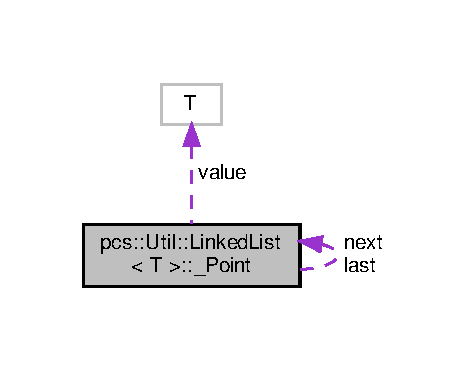
\includegraphics[width=224pt]{structpcs_1_1Util_1_1LinkedList_1_1__Point__coll__graph}
\end{center}
\end{figure}
\subsection*{Public Attributes}
\begin{DoxyCompactItemize}
\item 
T \hyperlink{structpcs_1_1Util_1_1LinkedList_1_1__Point_a2006e59eae181a2923dd28c3720c91d0}{value}
\item 
\hyperlink{structpcs_1_1Util_1_1LinkedList_1_1__Point}{\+\_\+\+Point} $\ast$ \hyperlink{structpcs_1_1Util_1_1LinkedList_1_1__Point_a7ce1b0f3d2380f944afd707b7a184b35}{last} = nullptr
\item 
\hyperlink{structpcs_1_1Util_1_1LinkedList_1_1__Point}{\+\_\+\+Point} $\ast$ \hyperlink{structpcs_1_1Util_1_1LinkedList_1_1__Point_ac6608e428bffcb2943d80aa962692cc4}{next} = nullptr
\end{DoxyCompactItemize}


\subsection{Member Data Documentation}
\mbox{\Hypertarget{structpcs_1_1Util_1_1LinkedList_1_1__Point_a7ce1b0f3d2380f944afd707b7a184b35}\label{structpcs_1_1Util_1_1LinkedList_1_1__Point_a7ce1b0f3d2380f944afd707b7a184b35}} 
\index{pcs\+::\+Util\+::\+Linked\+List\+::\+\_\+\+Point@{pcs\+::\+Util\+::\+Linked\+List\+::\+\_\+\+Point}!last@{last}}
\index{last@{last}!pcs\+::\+Util\+::\+Linked\+List\+::\+\_\+\+Point@{pcs\+::\+Util\+::\+Linked\+List\+::\+\_\+\+Point}}
\subsubsection{\texorpdfstring{last}{last}}
{\footnotesize\ttfamily template$<$typename T $>$ \\
\hyperlink{structpcs_1_1Util_1_1LinkedList_1_1__Point}{\+\_\+\+Point}$\ast$ \hyperlink{classpcs_1_1Util_1_1LinkedList}{pcs\+::\+Util\+::\+Linked\+List}$<$ T $>$\+::\+\_\+\+Point\+::last = nullptr}

\mbox{\Hypertarget{structpcs_1_1Util_1_1LinkedList_1_1__Point_ac6608e428bffcb2943d80aa962692cc4}\label{structpcs_1_1Util_1_1LinkedList_1_1__Point_ac6608e428bffcb2943d80aa962692cc4}} 
\index{pcs\+::\+Util\+::\+Linked\+List\+::\+\_\+\+Point@{pcs\+::\+Util\+::\+Linked\+List\+::\+\_\+\+Point}!next@{next}}
\index{next@{next}!pcs\+::\+Util\+::\+Linked\+List\+::\+\_\+\+Point@{pcs\+::\+Util\+::\+Linked\+List\+::\+\_\+\+Point}}
\subsubsection{\texorpdfstring{next}{next}}
{\footnotesize\ttfamily template$<$typename T $>$ \\
\hyperlink{structpcs_1_1Util_1_1LinkedList_1_1__Point}{\+\_\+\+Point}$\ast$ \hyperlink{classpcs_1_1Util_1_1LinkedList}{pcs\+::\+Util\+::\+Linked\+List}$<$ T $>$\+::\+\_\+\+Point\+::next = nullptr}

\mbox{\Hypertarget{structpcs_1_1Util_1_1LinkedList_1_1__Point_a2006e59eae181a2923dd28c3720c91d0}\label{structpcs_1_1Util_1_1LinkedList_1_1__Point_a2006e59eae181a2923dd28c3720c91d0}} 
\index{pcs\+::\+Util\+::\+Linked\+List\+::\+\_\+\+Point@{pcs\+::\+Util\+::\+Linked\+List\+::\+\_\+\+Point}!value@{value}}
\index{value@{value}!pcs\+::\+Util\+::\+Linked\+List\+::\+\_\+\+Point@{pcs\+::\+Util\+::\+Linked\+List\+::\+\_\+\+Point}}
\subsubsection{\texorpdfstring{value}{value}}
{\footnotesize\ttfamily template$<$typename T $>$ \\
T \hyperlink{classpcs_1_1Util_1_1LinkedList}{pcs\+::\+Util\+::\+Linked\+List}$<$ T $>$\+::\+\_\+\+Point\+::value}



The documentation for this struct was generated from the following file\+:\begin{DoxyCompactItemize}
\item 
include/\+Perceus/\+Util/\+Memory/\hyperlink{LinkedList_8h}{Linked\+List.\+h}\end{DoxyCompactItemize}

\hypertarget{classpcs_1_1Application}{}\section{pcs\+:\+:Application Class Reference}
\label{classpcs_1_1Application}\index{pcs\+::\+Application@{pcs\+::\+Application}}


Handles and runs the entire engine process. This is where the main loop is, this holds the engine.  




{\ttfamily \#include $<$Application.\+h$>$}



Inheritance diagram for pcs\+:\+:Application\+:\nopagebreak
\begin{figure}[H]
\begin{center}
\leavevmode
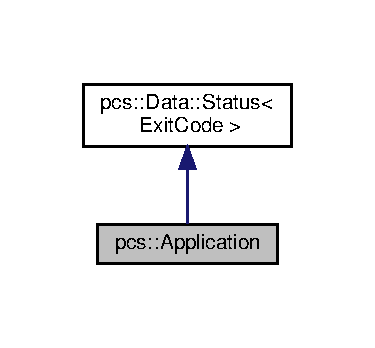
\includegraphics[width=180pt]{classpcs_1_1Application__inherit__graph}
\end{center}
\end{figure}


Collaboration diagram for pcs\+:\+:Application\+:
\nopagebreak
\begin{figure}[H]
\begin{center}
\leavevmode
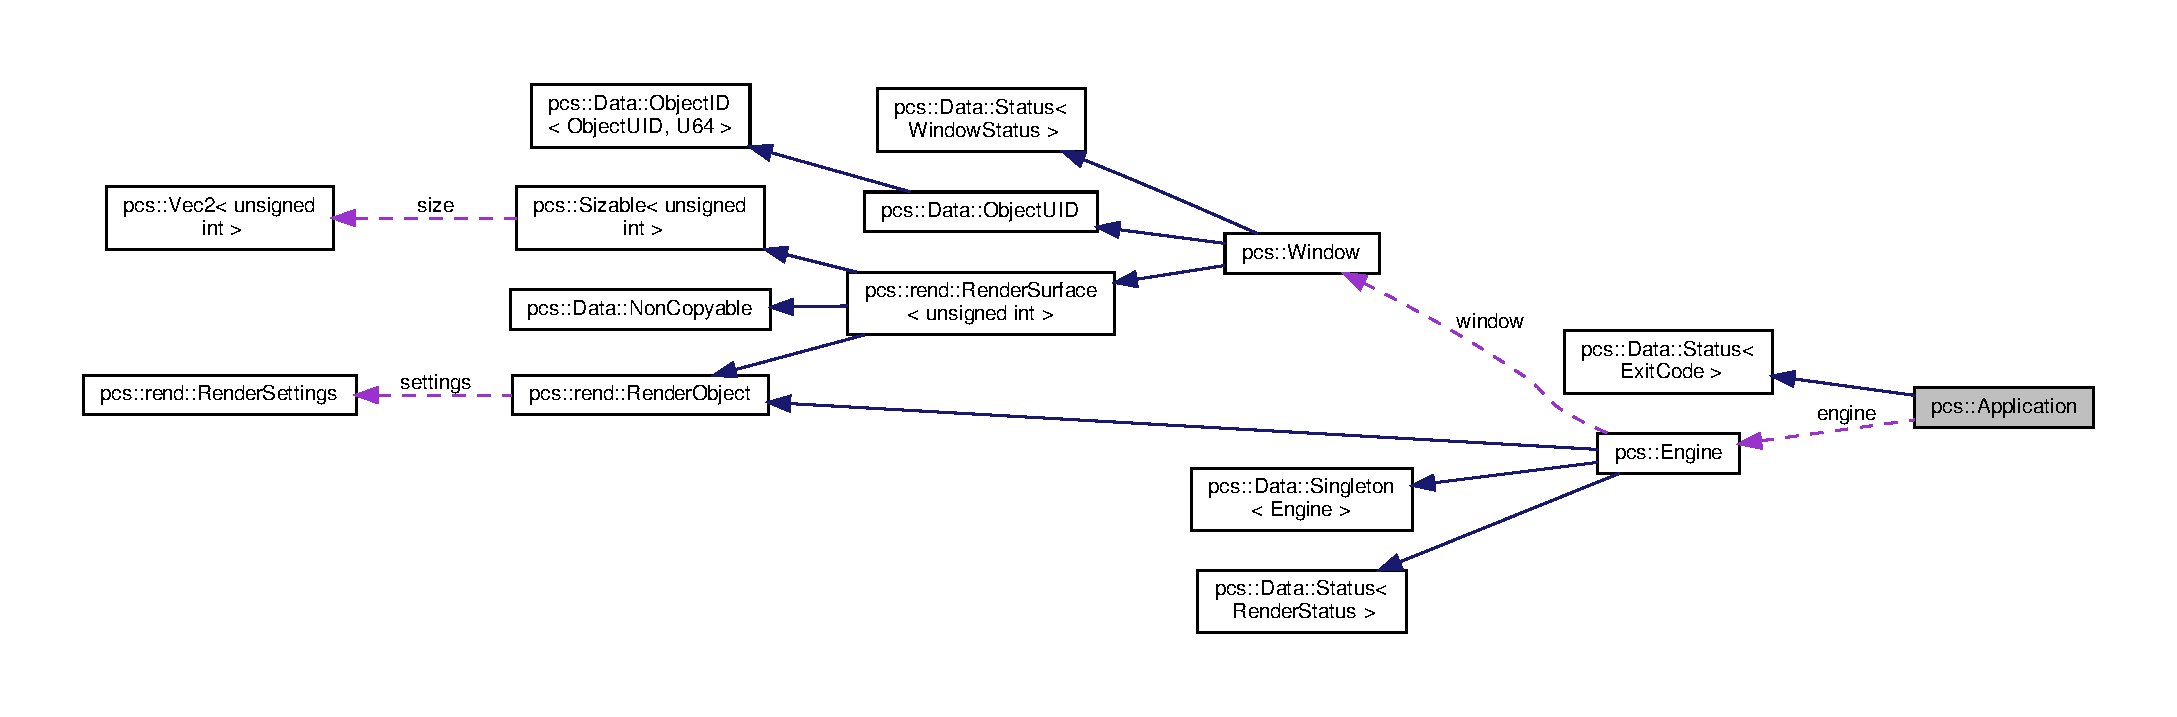
\includegraphics[width=350pt]{classpcs_1_1Application__coll__graph}
\end{center}
\end{figure}
\subsection*{Public Member Functions}
\begin{DoxyCompactItemize}
\item 
\hyperlink{classpcs_1_1Application_ad6c3666170e75e512603b3393c63ebd6}{Application} ()
\item 
virtual \hyperlink{classpcs_1_1Application_a3f81ec18fc0b79fd0ad9114fe020828d}{$\sim$\+Application} ()
\item 
int \hyperlink{classpcs_1_1Application_a00bc11d70a0aa5a8f7f5d03f357af712}{run} ()
\end{DoxyCompactItemize}
\subsection*{Protected Member Functions}
\begin{DoxyCompactItemize}
\item 
void \hyperlink{classpcs_1_1Application_ab840614431c7ad54bf09b684a07dba7e}{push\+Scene} (\hyperlink{classpcs_1_1Scene}{Scene} $\ast$s)
\end{DoxyCompactItemize}
\subsection*{Private Attributes}
\begin{DoxyCompactItemize}
\item 
\hyperlink{classpcs_1_1Engine}{Engine} $\ast$ \hyperlink{classpcs_1_1Application_a5d8a72ebc58019f9351926e04e079606}{engine}
\item 
std\+::stack$<$ \hyperlink{classpcs_1_1Scene}{Scene} $\ast$ $>$ \hyperlink{classpcs_1_1Application_afcc3279afd80bbe29841a54078401ce5}{scenes}
\end{DoxyCompactItemize}
\subsection*{Friends}
\begin{DoxyCompactItemize}
\item 
class \hyperlink{classpcs_1_1Application_a032858ae1fe02d2d1170981c2af2d67c}{Scene}
\end{DoxyCompactItemize}
\subsection*{Additional Inherited Members}


\subsection{Detailed Description}
Handles and runs the entire engine process. This is where the main loop is, this holds the engine. 

\subsection{Constructor \& Destructor Documentation}
\mbox{\Hypertarget{classpcs_1_1Application_ad6c3666170e75e512603b3393c63ebd6}\label{classpcs_1_1Application_ad6c3666170e75e512603b3393c63ebd6}} 
\index{pcs\+::\+Application@{pcs\+::\+Application}!Application@{Application}}
\index{Application@{Application}!pcs\+::\+Application@{pcs\+::\+Application}}
\subsubsection{\texorpdfstring{Application()}{Application()}}
{\footnotesize\ttfamily pcs\+::\+Application\+::\+Application (\begin{DoxyParamCaption}{ }\end{DoxyParamCaption})}

\mbox{\Hypertarget{classpcs_1_1Application_a3f81ec18fc0b79fd0ad9114fe020828d}\label{classpcs_1_1Application_a3f81ec18fc0b79fd0ad9114fe020828d}} 
\index{pcs\+::\+Application@{pcs\+::\+Application}!````~Application@{$\sim$\+Application}}
\index{````~Application@{$\sim$\+Application}!pcs\+::\+Application@{pcs\+::\+Application}}
\subsubsection{\texorpdfstring{$\sim$\+Application()}{~Application()}}
{\footnotesize\ttfamily pcs\+::\+Application\+::$\sim$\+Application (\begin{DoxyParamCaption}{ }\end{DoxyParamCaption})\hspace{0.3cm}{\ttfamily [virtual]}}



\subsection{Member Function Documentation}
\mbox{\Hypertarget{classpcs_1_1Application_ab840614431c7ad54bf09b684a07dba7e}\label{classpcs_1_1Application_ab840614431c7ad54bf09b684a07dba7e}} 
\index{pcs\+::\+Application@{pcs\+::\+Application}!push\+Scene@{push\+Scene}}
\index{push\+Scene@{push\+Scene}!pcs\+::\+Application@{pcs\+::\+Application}}
\subsubsection{\texorpdfstring{push\+Scene()}{pushScene()}}
{\footnotesize\ttfamily void pcs\+::\+Application\+::push\+Scene (\begin{DoxyParamCaption}\item[{\hyperlink{classpcs_1_1Scene}{Scene} $\ast$}]{s }\end{DoxyParamCaption})\hspace{0.3cm}{\ttfamily [protected]}}

\mbox{\Hypertarget{classpcs_1_1Application_a00bc11d70a0aa5a8f7f5d03f357af712}\label{classpcs_1_1Application_a00bc11d70a0aa5a8f7f5d03f357af712}} 
\index{pcs\+::\+Application@{pcs\+::\+Application}!run@{run}}
\index{run@{run}!pcs\+::\+Application@{pcs\+::\+Application}}
\subsubsection{\texorpdfstring{run()}{run()}}
{\footnotesize\ttfamily int pcs\+::\+Application\+::run (\begin{DoxyParamCaption}{ }\end{DoxyParamCaption})}



\subsection{Friends And Related Function Documentation}
\mbox{\Hypertarget{classpcs_1_1Application_a032858ae1fe02d2d1170981c2af2d67c}\label{classpcs_1_1Application_a032858ae1fe02d2d1170981c2af2d67c}} 
\index{pcs\+::\+Application@{pcs\+::\+Application}!Scene@{Scene}}
\index{Scene@{Scene}!pcs\+::\+Application@{pcs\+::\+Application}}
\subsubsection{\texorpdfstring{Scene}{Scene}}
{\footnotesize\ttfamily friend class \hyperlink{classpcs_1_1Scene}{Scene}\hspace{0.3cm}{\ttfamily [friend]}}



\subsection{Member Data Documentation}
\mbox{\Hypertarget{classpcs_1_1Application_a5d8a72ebc58019f9351926e04e079606}\label{classpcs_1_1Application_a5d8a72ebc58019f9351926e04e079606}} 
\index{pcs\+::\+Application@{pcs\+::\+Application}!engine@{engine}}
\index{engine@{engine}!pcs\+::\+Application@{pcs\+::\+Application}}
\subsubsection{\texorpdfstring{engine}{engine}}
{\footnotesize\ttfamily \hyperlink{classpcs_1_1Engine}{Engine}$\ast$ pcs\+::\+Application\+::engine\hspace{0.3cm}{\ttfamily [private]}}

\mbox{\Hypertarget{classpcs_1_1Application_afcc3279afd80bbe29841a54078401ce5}\label{classpcs_1_1Application_afcc3279afd80bbe29841a54078401ce5}} 
\index{pcs\+::\+Application@{pcs\+::\+Application}!scenes@{scenes}}
\index{scenes@{scenes}!pcs\+::\+Application@{pcs\+::\+Application}}
\subsubsection{\texorpdfstring{scenes}{scenes}}
{\footnotesize\ttfamily std\+::stack$<$\hyperlink{classpcs_1_1Scene}{Scene}$\ast$$>$ pcs\+::\+Application\+::scenes\hspace{0.3cm}{\ttfamily [private]}}



The documentation for this class was generated from the following files\+:\begin{DoxyCompactItemize}
\item 
include/\+Perceus/\+Core/\hyperlink{Application_8h}{Application.\+h}\item 
src/\+Core/\hyperlink{Application_8cpp}{Application.\+cpp}\end{DoxyCompactItemize}

\hypertarget{classpcs_1_1rend_1_1Buffer}{}\section{pcs\+:\+:rend\+:\+:Buffer Class Reference}
\label{classpcs_1_1rend_1_1Buffer}\index{pcs\+::rend\+::\+Buffer@{pcs\+::rend\+::\+Buffer}}


{\ttfamily \#include $<$Buffer.\+h$>$}



Inheritance diagram for pcs\+:\+:rend\+:\+:Buffer\+:\nopagebreak
\begin{figure}[H]
\begin{center}
\leavevmode
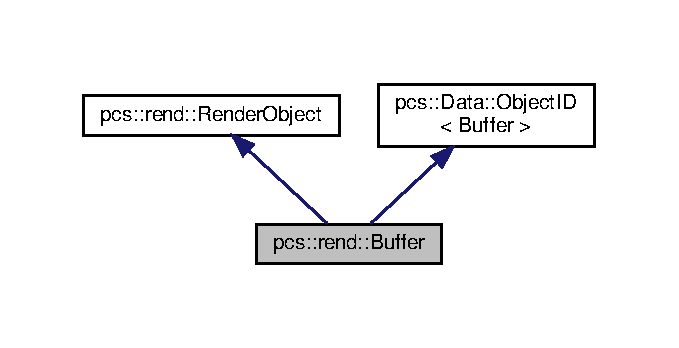
\includegraphics[width=326pt]{classpcs_1_1rend_1_1Buffer__inherit__graph}
\end{center}
\end{figure}


Collaboration diagram for pcs\+:\+:rend\+:\+:Buffer\+:\nopagebreak
\begin{figure}[H]
\begin{center}
\leavevmode
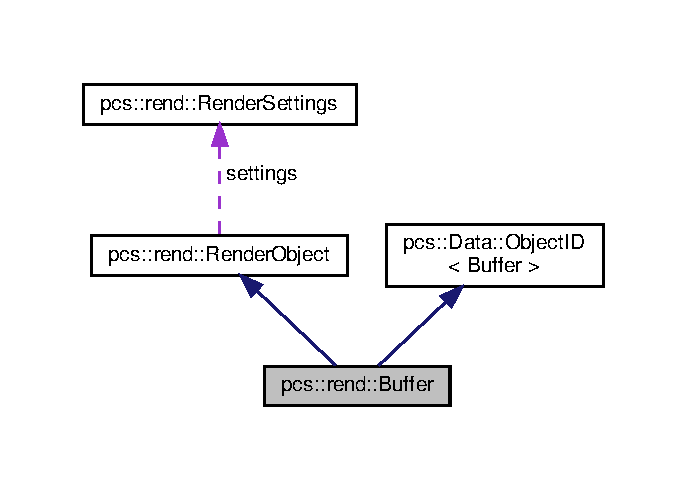
\includegraphics[width=330pt]{classpcs_1_1rend_1_1Buffer__coll__graph}
\end{center}
\end{figure}
\subsection*{Public Member Functions}
\begin{DoxyCompactItemize}
\item 
\hyperlink{classpcs_1_1rend_1_1Buffer_add9c4196c80605e47170fa37ad7eef50}{Buffer} (unsigned int index)
\item 
{\footnotesize template$<$typename... Args$>$ }\\\hyperlink{classpcs_1_1rend_1_1Buffer_a4ac6db7b29dd6a33d1f65b0c491a033f}{Buffer} (unsigned int index, Args... args)
\item 
\hyperlink{classpcs_1_1rend_1_1Buffer_a38bfdd852e494d21e430b2a0007021d4}{$\sim$\+Buffer} ()
\item 
void \hyperlink{classpcs_1_1rend_1_1Buffer_a1be9c6c19cee147e580c8d1038a664a9}{bind} ()
\item 
void \hyperlink{classpcs_1_1rend_1_1Buffer_ae50fade1bf8340f6db27af4bad5a09ba}{unbind} () const
\item 
{\footnotesize template$<$typename T $>$ }\\void \hyperlink{classpcs_1_1rend_1_1Buffer_a3e8a8fa6bbd51354ef27e86151d64022}{bind\+Data} (T $\ast$data, unsigned int count, unsigned int members)
\item 
{\footnotesize template$<$typename T $>$ }\\void \hyperlink{classpcs_1_1rend_1_1Buffer_ac121dc511109324c3d063799bbe8c81c}{bind\+Data} (std\+::vector$<$ T $>$ data, unsigned int members)
\item 
void \hyperlink{classpcs_1_1rend_1_1Buffer_a000af3de51f51ff6443da7ee4bdb0fe0}{bind\+Data} (std\+::vector$<$ \hyperlink{structpcs_1_1Mat4f}{Mat4f} $>$ \&matrices)
\item 
unsigned int \& \hyperlink{classpcs_1_1rend_1_1Buffer_a7825820bbf1227e6b94867523c6333fa}{get\+Index} ()
\item 
unsigned int \& \hyperlink{classpcs_1_1rend_1_1Buffer_a6b946389de081d61317561addc797356}{get\+Count} ()
\end{DoxyCompactItemize}
\subsection*{Private Attributes}
\begin{DoxyCompactItemize}
\item 
unsigned int \hyperlink{classpcs_1_1rend_1_1Buffer_ae651e17a3f64d982b2bd1e39e91bc89c}{\+\_\+index}
\item 
unsigned int \hyperlink{classpcs_1_1rend_1_1Buffer_a12efdd79f91856672f8c8dc8af0306c4}{\+\_\+count}
\end{DoxyCompactItemize}
\subsection*{Additional Inherited Members}


\subsection{Constructor \& Destructor Documentation}
\mbox{\Hypertarget{classpcs_1_1rend_1_1Buffer_add9c4196c80605e47170fa37ad7eef50}\label{classpcs_1_1rend_1_1Buffer_add9c4196c80605e47170fa37ad7eef50}} 
\index{pcs\+::rend\+::\+Buffer@{pcs\+::rend\+::\+Buffer}!Buffer@{Buffer}}
\index{Buffer@{Buffer}!pcs\+::rend\+::\+Buffer@{pcs\+::rend\+::\+Buffer}}
\subsubsection{\texorpdfstring{Buffer()}{Buffer()}\hspace{0.1cm}{\footnotesize\ttfamily [1/2]}}
{\footnotesize\ttfamily pcs\+::rend\+::\+Buffer\+::\+Buffer (\begin{DoxyParamCaption}\item[{unsigned int}]{index }\end{DoxyParamCaption})}

\mbox{\Hypertarget{classpcs_1_1rend_1_1Buffer_a4ac6db7b29dd6a33d1f65b0c491a033f}\label{classpcs_1_1rend_1_1Buffer_a4ac6db7b29dd6a33d1f65b0c491a033f}} 
\index{pcs\+::rend\+::\+Buffer@{pcs\+::rend\+::\+Buffer}!Buffer@{Buffer}}
\index{Buffer@{Buffer}!pcs\+::rend\+::\+Buffer@{pcs\+::rend\+::\+Buffer}}
\subsubsection{\texorpdfstring{Buffer()}{Buffer()}\hspace{0.1cm}{\footnotesize\ttfamily [2/2]}}
{\footnotesize\ttfamily template$<$typename... Args$>$ \\
pcs\+::rend\+::\+Buffer\+::\+Buffer (\begin{DoxyParamCaption}\item[{unsigned int}]{index,  }\item[{Args...}]{args }\end{DoxyParamCaption})\hspace{0.3cm}{\ttfamily [inline]}}

\mbox{\Hypertarget{classpcs_1_1rend_1_1Buffer_a38bfdd852e494d21e430b2a0007021d4}\label{classpcs_1_1rend_1_1Buffer_a38bfdd852e494d21e430b2a0007021d4}} 
\index{pcs\+::rend\+::\+Buffer@{pcs\+::rend\+::\+Buffer}!````~Buffer@{$\sim$\+Buffer}}
\index{````~Buffer@{$\sim$\+Buffer}!pcs\+::rend\+::\+Buffer@{pcs\+::rend\+::\+Buffer}}
\subsubsection{\texorpdfstring{$\sim$\+Buffer()}{~Buffer()}}
{\footnotesize\ttfamily pcs\+::rend\+::\+Buffer\+::$\sim$\+Buffer (\begin{DoxyParamCaption}{ }\end{DoxyParamCaption})}



\subsection{Member Function Documentation}
\mbox{\Hypertarget{classpcs_1_1rend_1_1Buffer_a1be9c6c19cee147e580c8d1038a664a9}\label{classpcs_1_1rend_1_1Buffer_a1be9c6c19cee147e580c8d1038a664a9}} 
\index{pcs\+::rend\+::\+Buffer@{pcs\+::rend\+::\+Buffer}!bind@{bind}}
\index{bind@{bind}!pcs\+::rend\+::\+Buffer@{pcs\+::rend\+::\+Buffer}}
\subsubsection{\texorpdfstring{bind()}{bind()}}
{\footnotesize\ttfamily void pcs\+::rend\+::\+Buffer\+::bind (\begin{DoxyParamCaption}{ }\end{DoxyParamCaption})}

\mbox{\Hypertarget{classpcs_1_1rend_1_1Buffer_a3e8a8fa6bbd51354ef27e86151d64022}\label{classpcs_1_1rend_1_1Buffer_a3e8a8fa6bbd51354ef27e86151d64022}} 
\index{pcs\+::rend\+::\+Buffer@{pcs\+::rend\+::\+Buffer}!bind\+Data@{bind\+Data}}
\index{bind\+Data@{bind\+Data}!pcs\+::rend\+::\+Buffer@{pcs\+::rend\+::\+Buffer}}
\subsubsection{\texorpdfstring{bind\+Data()}{bindData()}\hspace{0.1cm}{\footnotesize\ttfamily [1/3]}}
{\footnotesize\ttfamily template$<$typename T $>$ \\
void pcs\+::rend\+::\+Buffer\+::bind\+Data (\begin{DoxyParamCaption}\item[{T $\ast$}]{data,  }\item[{unsigned int}]{count,  }\item[{unsigned int}]{members }\end{DoxyParamCaption})\hspace{0.3cm}{\ttfamily [inline]}}

\mbox{\Hypertarget{classpcs_1_1rend_1_1Buffer_ac121dc511109324c3d063799bbe8c81c}\label{classpcs_1_1rend_1_1Buffer_ac121dc511109324c3d063799bbe8c81c}} 
\index{pcs\+::rend\+::\+Buffer@{pcs\+::rend\+::\+Buffer}!bind\+Data@{bind\+Data}}
\index{bind\+Data@{bind\+Data}!pcs\+::rend\+::\+Buffer@{pcs\+::rend\+::\+Buffer}}
\subsubsection{\texorpdfstring{bind\+Data()}{bindData()}\hspace{0.1cm}{\footnotesize\ttfamily [2/3]}}
{\footnotesize\ttfamily template$<$typename T $>$ \\
void pcs\+::rend\+::\+Buffer\+::bind\+Data (\begin{DoxyParamCaption}\item[{std\+::vector$<$ T $>$}]{data,  }\item[{unsigned int}]{members }\end{DoxyParamCaption})\hspace{0.3cm}{\ttfamily [inline]}}

\mbox{\Hypertarget{classpcs_1_1rend_1_1Buffer_a000af3de51f51ff6443da7ee4bdb0fe0}\label{classpcs_1_1rend_1_1Buffer_a000af3de51f51ff6443da7ee4bdb0fe0}} 
\index{pcs\+::rend\+::\+Buffer@{pcs\+::rend\+::\+Buffer}!bind\+Data@{bind\+Data}}
\index{bind\+Data@{bind\+Data}!pcs\+::rend\+::\+Buffer@{pcs\+::rend\+::\+Buffer}}
\subsubsection{\texorpdfstring{bind\+Data()}{bindData()}\hspace{0.1cm}{\footnotesize\ttfamily [3/3]}}
{\footnotesize\ttfamily void pcs\+::rend\+::\+Buffer\+::bind\+Data (\begin{DoxyParamCaption}\item[{std\+::vector$<$ \hyperlink{structpcs_1_1Mat4f}{Mat4f} $>$ \&}]{matrices }\end{DoxyParamCaption})\hspace{0.3cm}{\ttfamily [inline]}}

\mbox{\Hypertarget{classpcs_1_1rend_1_1Buffer_a6b946389de081d61317561addc797356}\label{classpcs_1_1rend_1_1Buffer_a6b946389de081d61317561addc797356}} 
\index{pcs\+::rend\+::\+Buffer@{pcs\+::rend\+::\+Buffer}!get\+Count@{get\+Count}}
\index{get\+Count@{get\+Count}!pcs\+::rend\+::\+Buffer@{pcs\+::rend\+::\+Buffer}}
\subsubsection{\texorpdfstring{get\+Count()}{getCount()}}
{\footnotesize\ttfamily unsigned int\& pcs\+::rend\+::\+Buffer\+::get\+Count (\begin{DoxyParamCaption}{ }\end{DoxyParamCaption})\hspace{0.3cm}{\ttfamily [inline]}}

\mbox{\Hypertarget{classpcs_1_1rend_1_1Buffer_a7825820bbf1227e6b94867523c6333fa}\label{classpcs_1_1rend_1_1Buffer_a7825820bbf1227e6b94867523c6333fa}} 
\index{pcs\+::rend\+::\+Buffer@{pcs\+::rend\+::\+Buffer}!get\+Index@{get\+Index}}
\index{get\+Index@{get\+Index}!pcs\+::rend\+::\+Buffer@{pcs\+::rend\+::\+Buffer}}
\subsubsection{\texorpdfstring{get\+Index()}{getIndex()}}
{\footnotesize\ttfamily unsigned int\& pcs\+::rend\+::\+Buffer\+::get\+Index (\begin{DoxyParamCaption}{ }\end{DoxyParamCaption})\hspace{0.3cm}{\ttfamily [inline]}}

\mbox{\Hypertarget{classpcs_1_1rend_1_1Buffer_ae50fade1bf8340f6db27af4bad5a09ba}\label{classpcs_1_1rend_1_1Buffer_ae50fade1bf8340f6db27af4bad5a09ba}} 
\index{pcs\+::rend\+::\+Buffer@{pcs\+::rend\+::\+Buffer}!unbind@{unbind}}
\index{unbind@{unbind}!pcs\+::rend\+::\+Buffer@{pcs\+::rend\+::\+Buffer}}
\subsubsection{\texorpdfstring{unbind()}{unbind()}}
{\footnotesize\ttfamily void pcs\+::rend\+::\+Buffer\+::unbind (\begin{DoxyParamCaption}{ }\end{DoxyParamCaption}) const}



\subsection{Member Data Documentation}
\mbox{\Hypertarget{classpcs_1_1rend_1_1Buffer_a12efdd79f91856672f8c8dc8af0306c4}\label{classpcs_1_1rend_1_1Buffer_a12efdd79f91856672f8c8dc8af0306c4}} 
\index{pcs\+::rend\+::\+Buffer@{pcs\+::rend\+::\+Buffer}!\+\_\+count@{\+\_\+count}}
\index{\+\_\+count@{\+\_\+count}!pcs\+::rend\+::\+Buffer@{pcs\+::rend\+::\+Buffer}}
\subsubsection{\texorpdfstring{\+\_\+count}{\_count}}
{\footnotesize\ttfamily unsigned int pcs\+::rend\+::\+Buffer\+::\+\_\+count\hspace{0.3cm}{\ttfamily [private]}}

\mbox{\Hypertarget{classpcs_1_1rend_1_1Buffer_ae651e17a3f64d982b2bd1e39e91bc89c}\label{classpcs_1_1rend_1_1Buffer_ae651e17a3f64d982b2bd1e39e91bc89c}} 
\index{pcs\+::rend\+::\+Buffer@{pcs\+::rend\+::\+Buffer}!\+\_\+index@{\+\_\+index}}
\index{\+\_\+index@{\+\_\+index}!pcs\+::rend\+::\+Buffer@{pcs\+::rend\+::\+Buffer}}
\subsubsection{\texorpdfstring{\+\_\+index}{\_index}}
{\footnotesize\ttfamily unsigned int pcs\+::rend\+::\+Buffer\+::\+\_\+index\hspace{0.3cm}{\ttfamily [private]}}



The documentation for this class was generated from the following files\+:\begin{DoxyCompactItemize}
\item 
include/\+Perceus/\+Core/\+Graphics/\+Entities/\hyperlink{Buffer_8h}{Buffer.\+h}\item 
src/\+Core/\+Graphics/\+Entities/\hyperlink{Buffer_8cpp}{Buffer.\+cpp}\end{DoxyCompactItemize}

\hypertarget{classpcs_1_1rend_1_1BufferArray}{}\section{pcs\+:\+:rend\+:\+:Buffer\+Array Class Reference}
\label{classpcs_1_1rend_1_1BufferArray}\index{pcs\+::rend\+::\+Buffer\+Array@{pcs\+::rend\+::\+Buffer\+Array}}


{\ttfamily \#include $<$Buffer\+Array.\+h$>$}



Inheritance diagram for pcs\+:\+:rend\+:\+:Buffer\+Array\+:\nopagebreak
\begin{figure}[H]
\begin{center}
\leavevmode
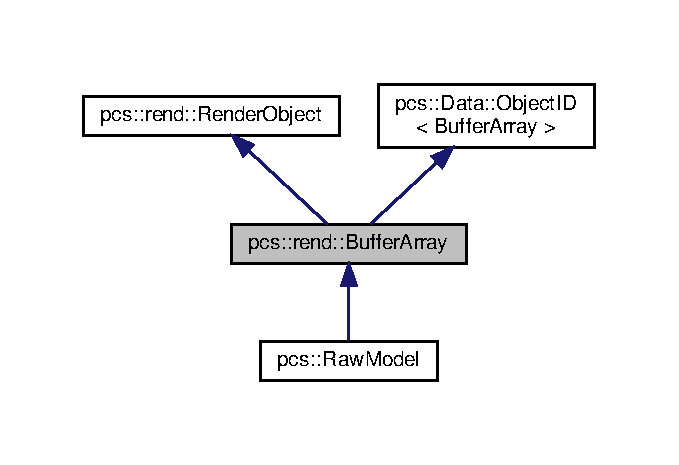
\includegraphics[width=326pt]{classpcs_1_1rend_1_1BufferArray__inherit__graph}
\end{center}
\end{figure}


Collaboration diagram for pcs\+:\+:rend\+:\+:Buffer\+Array\+:\nopagebreak
\begin{figure}[H]
\begin{center}
\leavevmode
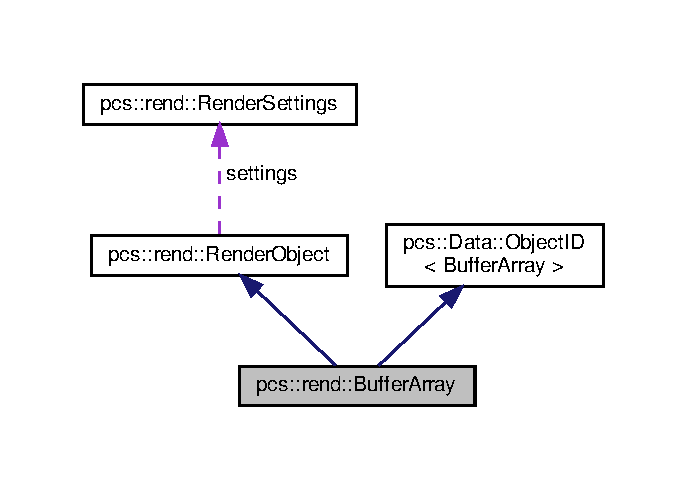
\includegraphics[width=330pt]{classpcs_1_1rend_1_1BufferArray__coll__graph}
\end{center}
\end{figure}
\subsection*{Public Member Functions}
\begin{DoxyCompactItemize}
\item 
\hyperlink{classpcs_1_1rend_1_1BufferArray_a8e4885f9616165139b318a1b879691e5}{Buffer\+Array} ()
\item 
virtual \hyperlink{classpcs_1_1rend_1_1BufferArray_a4492755723fc99752c811bfe7520d993}{$\sim$\+Buffer\+Array} ()
\item 
\hyperlink{classpcs_1_1rend_1_1Buffer}{Buffer} \& \hyperlink{classpcs_1_1rend_1_1BufferArray_ad4b43fddb8e19fcaa6fbb8ff80a64a94}{get\+Buffer} (\hyperlink{namespacepcs_1_1rend_a731e43a479c7b7b61dd23586494ee61b}{Buffer\+Index} buffer)
\item 
void \hyperlink{classpcs_1_1rend_1_1BufferArray_ab170f51886678c0c027acdf604915eb7}{bind} () const
\item 
void \hyperlink{classpcs_1_1rend_1_1BufferArray_a8c00f92e0911c209b26cf99fa2920d95}{unbind} () const
\end{DoxyCompactItemize}
\subsection*{Static Public Member Functions}
\begin{DoxyCompactItemize}
\item 
static const char $\ast$ \hyperlink{classpcs_1_1rend_1_1BufferArray_a7ed1705d18349b1e7a08b769f233546a}{get\+Buffer\+Name} (unsigned int index)
\end{DoxyCompactItemize}
\subsection*{Protected Member Functions}
\begin{DoxyCompactItemize}
\item 
{\footnotesize template$<$typename T $>$ }\\void \hyperlink{classpcs_1_1rend_1_1BufferArray_ad31f62704dd0b4c4b6097681aa06c00b}{bind\+Buffer} (\hyperlink{namespacepcs_1_1rend_a731e43a479c7b7b61dd23586494ee61b}{Buffer\+Index} buffer, unsigned int members, std\+::vector$<$ T $>$ \&data)
\item 
void \hyperlink{classpcs_1_1rend_1_1BufferArray_a1f07a68045a6772619641b6059668d34}{bind\+Buffer} (std\+::vector$<$ \hyperlink{structpcs_1_1Mat4f}{Mat4f} $>$ \&data)
\end{DoxyCompactItemize}
\subsection*{Private Attributes}
\begin{DoxyCompactItemize}
\item 
std\+::vector$<$ \hyperlink{classpcs_1_1rend_1_1Buffer}{Buffer} $\ast$ $>$ \hyperlink{classpcs_1_1rend_1_1BufferArray_a9e2281d3dab3361dd8b9aca55c53e4a7}{buffers}
\end{DoxyCompactItemize}
\subsection*{Additional Inherited Members}


\subsection{Constructor \& Destructor Documentation}
\mbox{\Hypertarget{classpcs_1_1rend_1_1BufferArray_a8e4885f9616165139b318a1b879691e5}\label{classpcs_1_1rend_1_1BufferArray_a8e4885f9616165139b318a1b879691e5}} 
\index{pcs\+::rend\+::\+Buffer\+Array@{pcs\+::rend\+::\+Buffer\+Array}!Buffer\+Array@{Buffer\+Array}}
\index{Buffer\+Array@{Buffer\+Array}!pcs\+::rend\+::\+Buffer\+Array@{pcs\+::rend\+::\+Buffer\+Array}}
\subsubsection{\texorpdfstring{Buffer\+Array()}{BufferArray()}}
{\footnotesize\ttfamily pcs\+::rend\+::\+Buffer\+Array\+::\+Buffer\+Array (\begin{DoxyParamCaption}{ }\end{DoxyParamCaption})}

\mbox{\Hypertarget{classpcs_1_1rend_1_1BufferArray_a4492755723fc99752c811bfe7520d993}\label{classpcs_1_1rend_1_1BufferArray_a4492755723fc99752c811bfe7520d993}} 
\index{pcs\+::rend\+::\+Buffer\+Array@{pcs\+::rend\+::\+Buffer\+Array}!````~Buffer\+Array@{$\sim$\+Buffer\+Array}}
\index{````~Buffer\+Array@{$\sim$\+Buffer\+Array}!pcs\+::rend\+::\+Buffer\+Array@{pcs\+::rend\+::\+Buffer\+Array}}
\subsubsection{\texorpdfstring{$\sim$\+Buffer\+Array()}{~BufferArray()}}
{\footnotesize\ttfamily pcs\+::rend\+::\+Buffer\+Array\+::$\sim$\+Buffer\+Array (\begin{DoxyParamCaption}{ }\end{DoxyParamCaption})\hspace{0.3cm}{\ttfamily [virtual]}}



\subsection{Member Function Documentation}
\mbox{\Hypertarget{classpcs_1_1rend_1_1BufferArray_ab170f51886678c0c027acdf604915eb7}\label{classpcs_1_1rend_1_1BufferArray_ab170f51886678c0c027acdf604915eb7}} 
\index{pcs\+::rend\+::\+Buffer\+Array@{pcs\+::rend\+::\+Buffer\+Array}!bind@{bind}}
\index{bind@{bind}!pcs\+::rend\+::\+Buffer\+Array@{pcs\+::rend\+::\+Buffer\+Array}}
\subsubsection{\texorpdfstring{bind()}{bind()}}
{\footnotesize\ttfamily void pcs\+::rend\+::\+Buffer\+Array\+::bind (\begin{DoxyParamCaption}{ }\end{DoxyParamCaption}) const\hspace{0.3cm}{\ttfamily [inline]}}

\mbox{\Hypertarget{classpcs_1_1rend_1_1BufferArray_ad31f62704dd0b4c4b6097681aa06c00b}\label{classpcs_1_1rend_1_1BufferArray_ad31f62704dd0b4c4b6097681aa06c00b}} 
\index{pcs\+::rend\+::\+Buffer\+Array@{pcs\+::rend\+::\+Buffer\+Array}!bind\+Buffer@{bind\+Buffer}}
\index{bind\+Buffer@{bind\+Buffer}!pcs\+::rend\+::\+Buffer\+Array@{pcs\+::rend\+::\+Buffer\+Array}}
\subsubsection{\texorpdfstring{bind\+Buffer()}{bindBuffer()}\hspace{0.1cm}{\footnotesize\ttfamily [1/2]}}
{\footnotesize\ttfamily template$<$typename T $>$ \\
void pcs\+::rend\+::\+Buffer\+Array\+::bind\+Buffer (\begin{DoxyParamCaption}\item[{\hyperlink{namespacepcs_1_1rend_a731e43a479c7b7b61dd23586494ee61b}{Buffer\+Index}}]{buffer,  }\item[{unsigned int}]{members,  }\item[{std\+::vector$<$ T $>$ \&}]{data }\end{DoxyParamCaption})\hspace{0.3cm}{\ttfamily [inline]}, {\ttfamily [protected]}}

\mbox{\Hypertarget{classpcs_1_1rend_1_1BufferArray_a1f07a68045a6772619641b6059668d34}\label{classpcs_1_1rend_1_1BufferArray_a1f07a68045a6772619641b6059668d34}} 
\index{pcs\+::rend\+::\+Buffer\+Array@{pcs\+::rend\+::\+Buffer\+Array}!bind\+Buffer@{bind\+Buffer}}
\index{bind\+Buffer@{bind\+Buffer}!pcs\+::rend\+::\+Buffer\+Array@{pcs\+::rend\+::\+Buffer\+Array}}
\subsubsection{\texorpdfstring{bind\+Buffer()}{bindBuffer()}\hspace{0.1cm}{\footnotesize\ttfamily [2/2]}}
{\footnotesize\ttfamily void pcs\+::rend\+::\+Buffer\+Array\+::bind\+Buffer (\begin{DoxyParamCaption}\item[{std\+::vector$<$ \hyperlink{structpcs_1_1Mat4f}{Mat4f} $>$ \&}]{data }\end{DoxyParamCaption})\hspace{0.3cm}{\ttfamily [inline]}, {\ttfamily [protected]}}

\mbox{\Hypertarget{classpcs_1_1rend_1_1BufferArray_ad4b43fddb8e19fcaa6fbb8ff80a64a94}\label{classpcs_1_1rend_1_1BufferArray_ad4b43fddb8e19fcaa6fbb8ff80a64a94}} 
\index{pcs\+::rend\+::\+Buffer\+Array@{pcs\+::rend\+::\+Buffer\+Array}!get\+Buffer@{get\+Buffer}}
\index{get\+Buffer@{get\+Buffer}!pcs\+::rend\+::\+Buffer\+Array@{pcs\+::rend\+::\+Buffer\+Array}}
\subsubsection{\texorpdfstring{get\+Buffer()}{getBuffer()}}
{\footnotesize\ttfamily \hyperlink{classpcs_1_1rend_1_1Buffer}{Buffer}\& pcs\+::rend\+::\+Buffer\+Array\+::get\+Buffer (\begin{DoxyParamCaption}\item[{\hyperlink{namespacepcs_1_1rend_a731e43a479c7b7b61dd23586494ee61b}{Buffer\+Index}}]{buffer }\end{DoxyParamCaption})\hspace{0.3cm}{\ttfamily [inline]}}

\mbox{\Hypertarget{classpcs_1_1rend_1_1BufferArray_a7ed1705d18349b1e7a08b769f233546a}\label{classpcs_1_1rend_1_1BufferArray_a7ed1705d18349b1e7a08b769f233546a}} 
\index{pcs\+::rend\+::\+Buffer\+Array@{pcs\+::rend\+::\+Buffer\+Array}!get\+Buffer\+Name@{get\+Buffer\+Name}}
\index{get\+Buffer\+Name@{get\+Buffer\+Name}!pcs\+::rend\+::\+Buffer\+Array@{pcs\+::rend\+::\+Buffer\+Array}}
\subsubsection{\texorpdfstring{get\+Buffer\+Name()}{getBufferName()}}
{\footnotesize\ttfamily static const char$\ast$ pcs\+::rend\+::\+Buffer\+Array\+::get\+Buffer\+Name (\begin{DoxyParamCaption}\item[{unsigned int}]{index }\end{DoxyParamCaption})\hspace{0.3cm}{\ttfamily [inline]}, {\ttfamily [static]}}

\mbox{\Hypertarget{classpcs_1_1rend_1_1BufferArray_a8c00f92e0911c209b26cf99fa2920d95}\label{classpcs_1_1rend_1_1BufferArray_a8c00f92e0911c209b26cf99fa2920d95}} 
\index{pcs\+::rend\+::\+Buffer\+Array@{pcs\+::rend\+::\+Buffer\+Array}!unbind@{unbind}}
\index{unbind@{unbind}!pcs\+::rend\+::\+Buffer\+Array@{pcs\+::rend\+::\+Buffer\+Array}}
\subsubsection{\texorpdfstring{unbind()}{unbind()}}
{\footnotesize\ttfamily void pcs\+::rend\+::\+Buffer\+Array\+::unbind (\begin{DoxyParamCaption}{ }\end{DoxyParamCaption}) const\hspace{0.3cm}{\ttfamily [inline]}}



\subsection{Member Data Documentation}
\mbox{\Hypertarget{classpcs_1_1rend_1_1BufferArray_a9e2281d3dab3361dd8b9aca55c53e4a7}\label{classpcs_1_1rend_1_1BufferArray_a9e2281d3dab3361dd8b9aca55c53e4a7}} 
\index{pcs\+::rend\+::\+Buffer\+Array@{pcs\+::rend\+::\+Buffer\+Array}!buffers@{buffers}}
\index{buffers@{buffers}!pcs\+::rend\+::\+Buffer\+Array@{pcs\+::rend\+::\+Buffer\+Array}}
\subsubsection{\texorpdfstring{buffers}{buffers}}
{\footnotesize\ttfamily std\+::vector$<$\hyperlink{classpcs_1_1rend_1_1Buffer}{Buffer}$\ast$$>$ pcs\+::rend\+::\+Buffer\+Array\+::buffers\hspace{0.3cm}{\ttfamily [private]}}



The documentation for this class was generated from the following files\+:\begin{DoxyCompactItemize}
\item 
include/\+Perceus/\+Core/\+Graphics/\+Entities/\hyperlink{BufferArray_8h}{Buffer\+Array.\+h}\item 
src/\+Core/\+Graphics/\+Entities/\hyperlink{BufferArray_8cpp}{Buffer\+Array.\+cpp}\end{DoxyCompactItemize}

\hypertarget{classpcs_1_1Camera}{}\section{pcs\+:\+:Camera Class Reference}
\label{classpcs_1_1Camera}\index{pcs\+::\+Camera@{pcs\+::\+Camera}}


{\ttfamily \#include $<$Camera.\+h$>$}



Inheritance diagram for pcs\+:\+:Camera\+:\nopagebreak
\begin{figure}[H]
\begin{center}
\leavevmode
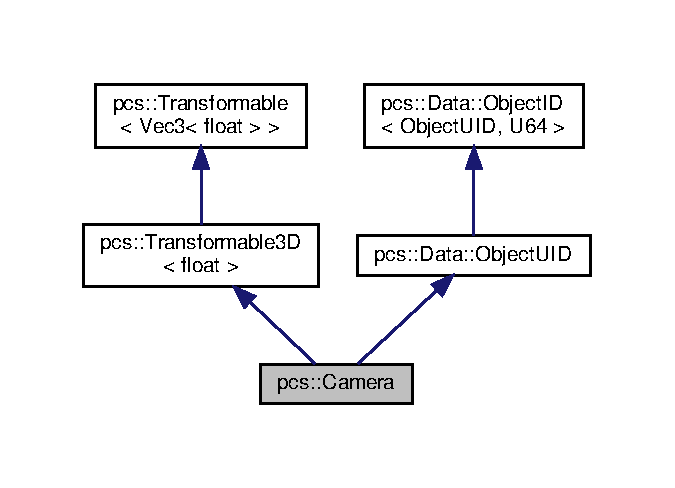
\includegraphics[width=324pt]{classpcs_1_1Camera__inherit__graph}
\end{center}
\end{figure}


Collaboration diagram for pcs\+:\+:Camera\+:\nopagebreak
\begin{figure}[H]
\begin{center}
\leavevmode
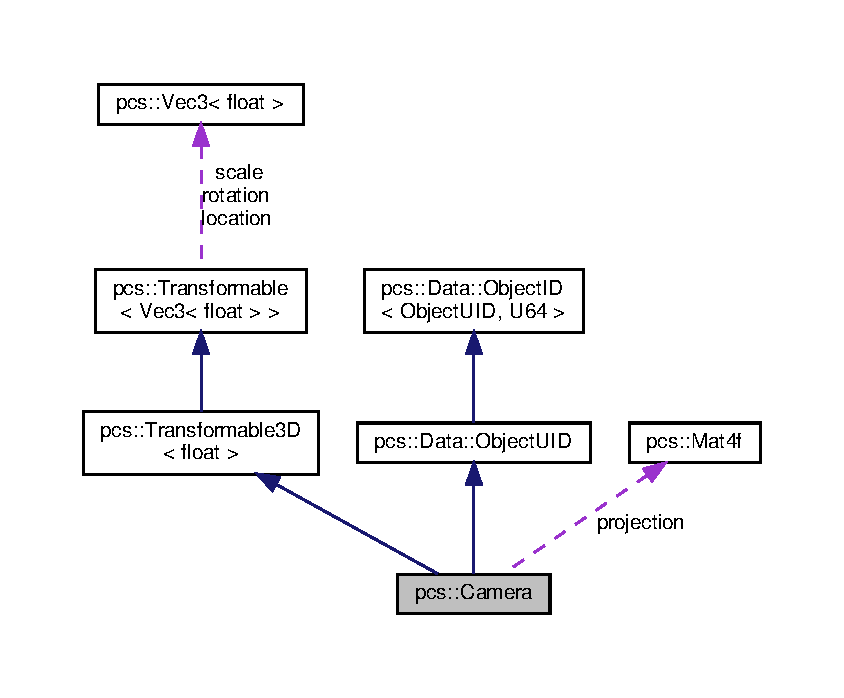
\includegraphics[width=350pt]{classpcs_1_1Camera__coll__graph}
\end{center}
\end{figure}
\subsection*{Public Member Functions}
\begin{DoxyCompactItemize}
\item 
\hyperlink{classpcs_1_1Camera_ac45030bc986f4d5f4d029d1750a8bb9a}{Camera} (float F\+OV=90.f, float z\+Near=.\+01f, float z\+Far=1000.\+f)
\item 
\hyperlink{classpcs_1_1Camera_ad46170506d099a71fd7f025a82405310}{$\sim$\+Camera} ()
\item 
\hyperlink{structpcs_1_1Mat4f}{Mat4f} \hyperlink{classpcs_1_1Camera_afb48cb746e7d789dc0395009fd0d03b5}{get\+View} ()
\item 
\hyperlink{structpcs_1_1Mat4f}{Mat4f} \hyperlink{classpcs_1_1Camera_a54785d1551fb6d273f77b6bcf806837b}{get\+Projection} () const
\item 
void \hyperlink{classpcs_1_1Camera_af43d459cebd61a86a492d632e2b4bd14}{associate\+Window} (\hyperlink{classpcs_1_1Window}{Window} $\ast$win)
\item 
void \hyperlink{classpcs_1_1Camera_a7595a6bbed4b3608cb264ff1a16b6516}{make\+Projection} (float F\+OV=-\/1, float z\+Near=-\/11, float z\+Far=-\/1)
\end{DoxyCompactItemize}
\subsection*{Private Attributes}
\begin{DoxyCompactItemize}
\item 
\hyperlink{structpcs_1_1Mat4f}{Mat4f} \hyperlink{classpcs_1_1Camera_ae70659a115f743ad3da47e10a52c24b3}{projection}
\item 
float \hyperlink{classpcs_1_1Camera_a604debcdfaf49edd5a9d513e7c0ed880}{\+\_\+\+F\+OV}
\item 
float \hyperlink{classpcs_1_1Camera_a5ecff3330616665cb449d3e687373d7d}{\+\_\+z\+Near}
\item 
float \hyperlink{classpcs_1_1Camera_a4f072907820f923c48a5e875c9b05f7b}{\+\_\+z\+Far}
\end{DoxyCompactItemize}
\subsection*{Additional Inherited Members}


\subsection{Constructor \& Destructor Documentation}
\mbox{\Hypertarget{classpcs_1_1Camera_ac45030bc986f4d5f4d029d1750a8bb9a}\label{classpcs_1_1Camera_ac45030bc986f4d5f4d029d1750a8bb9a}} 
\index{pcs\+::\+Camera@{pcs\+::\+Camera}!Camera@{Camera}}
\index{Camera@{Camera}!pcs\+::\+Camera@{pcs\+::\+Camera}}
\subsubsection{\texorpdfstring{Camera()}{Camera()}}
{\footnotesize\ttfamily pcs\+::\+Camera\+::\+Camera (\begin{DoxyParamCaption}\item[{float}]{F\+OV = {\ttfamily 90.f},  }\item[{float}]{z\+Near = {\ttfamily .01f},  }\item[{float}]{z\+Far = {\ttfamily 1000.f} }\end{DoxyParamCaption})}

\mbox{\Hypertarget{classpcs_1_1Camera_ad46170506d099a71fd7f025a82405310}\label{classpcs_1_1Camera_ad46170506d099a71fd7f025a82405310}} 
\index{pcs\+::\+Camera@{pcs\+::\+Camera}!````~Camera@{$\sim$\+Camera}}
\index{````~Camera@{$\sim$\+Camera}!pcs\+::\+Camera@{pcs\+::\+Camera}}
\subsubsection{\texorpdfstring{$\sim$\+Camera()}{~Camera()}}
{\footnotesize\ttfamily pcs\+::\+Camera\+::$\sim$\+Camera (\begin{DoxyParamCaption}{ }\end{DoxyParamCaption})\hspace{0.3cm}{\ttfamily [inline]}}



\subsection{Member Function Documentation}
\mbox{\Hypertarget{classpcs_1_1Camera_af43d459cebd61a86a492d632e2b4bd14}\label{classpcs_1_1Camera_af43d459cebd61a86a492d632e2b4bd14}} 
\index{pcs\+::\+Camera@{pcs\+::\+Camera}!associate\+Window@{associate\+Window}}
\index{associate\+Window@{associate\+Window}!pcs\+::\+Camera@{pcs\+::\+Camera}}
\subsubsection{\texorpdfstring{associate\+Window()}{associateWindow()}}
{\footnotesize\ttfamily void pcs\+::\+Camera\+::associate\+Window (\begin{DoxyParamCaption}\item[{\hyperlink{classpcs_1_1Window}{Window} $\ast$}]{win }\end{DoxyParamCaption})}

\mbox{\Hypertarget{classpcs_1_1Camera_a54785d1551fb6d273f77b6bcf806837b}\label{classpcs_1_1Camera_a54785d1551fb6d273f77b6bcf806837b}} 
\index{pcs\+::\+Camera@{pcs\+::\+Camera}!get\+Projection@{get\+Projection}}
\index{get\+Projection@{get\+Projection}!pcs\+::\+Camera@{pcs\+::\+Camera}}
\subsubsection{\texorpdfstring{get\+Projection()}{getProjection()}}
{\footnotesize\ttfamily \hyperlink{structpcs_1_1Mat4f}{Mat4f} pcs\+::\+Camera\+::get\+Projection (\begin{DoxyParamCaption}{ }\end{DoxyParamCaption}) const\hspace{0.3cm}{\ttfamily [inline]}}

\mbox{\Hypertarget{classpcs_1_1Camera_afb48cb746e7d789dc0395009fd0d03b5}\label{classpcs_1_1Camera_afb48cb746e7d789dc0395009fd0d03b5}} 
\index{pcs\+::\+Camera@{pcs\+::\+Camera}!get\+View@{get\+View}}
\index{get\+View@{get\+View}!pcs\+::\+Camera@{pcs\+::\+Camera}}
\subsubsection{\texorpdfstring{get\+View()}{getView()}}
{\footnotesize\ttfamily \hyperlink{structpcs_1_1Mat4f}{Mat4f} pcs\+::\+Camera\+::get\+View (\begin{DoxyParamCaption}{ }\end{DoxyParamCaption})}

\mbox{\Hypertarget{classpcs_1_1Camera_a7595a6bbed4b3608cb264ff1a16b6516}\label{classpcs_1_1Camera_a7595a6bbed4b3608cb264ff1a16b6516}} 
\index{pcs\+::\+Camera@{pcs\+::\+Camera}!make\+Projection@{make\+Projection}}
\index{make\+Projection@{make\+Projection}!pcs\+::\+Camera@{pcs\+::\+Camera}}
\subsubsection{\texorpdfstring{make\+Projection()}{makeProjection()}}
{\footnotesize\ttfamily void pcs\+::\+Camera\+::make\+Projection (\begin{DoxyParamCaption}\item[{float}]{F\+OV = {\ttfamily -\/1},  }\item[{float}]{z\+Near = {\ttfamily -\/11},  }\item[{float}]{z\+Far = {\ttfamily -\/1} }\end{DoxyParamCaption})}



\subsection{Member Data Documentation}
\mbox{\Hypertarget{classpcs_1_1Camera_a604debcdfaf49edd5a9d513e7c0ed880}\label{classpcs_1_1Camera_a604debcdfaf49edd5a9d513e7c0ed880}} 
\index{pcs\+::\+Camera@{pcs\+::\+Camera}!\+\_\+\+F\+OV@{\+\_\+\+F\+OV}}
\index{\+\_\+\+F\+OV@{\+\_\+\+F\+OV}!pcs\+::\+Camera@{pcs\+::\+Camera}}
\subsubsection{\texorpdfstring{\+\_\+\+F\+OV}{\_FOV}}
{\footnotesize\ttfamily float pcs\+::\+Camera\+::\+\_\+\+F\+OV\hspace{0.3cm}{\ttfamily [private]}}

\mbox{\Hypertarget{classpcs_1_1Camera_a4f072907820f923c48a5e875c9b05f7b}\label{classpcs_1_1Camera_a4f072907820f923c48a5e875c9b05f7b}} 
\index{pcs\+::\+Camera@{pcs\+::\+Camera}!\+\_\+z\+Far@{\+\_\+z\+Far}}
\index{\+\_\+z\+Far@{\+\_\+z\+Far}!pcs\+::\+Camera@{pcs\+::\+Camera}}
\subsubsection{\texorpdfstring{\+\_\+z\+Far}{\_zFar}}
{\footnotesize\ttfamily float pcs\+::\+Camera\+::\+\_\+z\+Far\hspace{0.3cm}{\ttfamily [private]}}

\mbox{\Hypertarget{classpcs_1_1Camera_a5ecff3330616665cb449d3e687373d7d}\label{classpcs_1_1Camera_a5ecff3330616665cb449d3e687373d7d}} 
\index{pcs\+::\+Camera@{pcs\+::\+Camera}!\+\_\+z\+Near@{\+\_\+z\+Near}}
\index{\+\_\+z\+Near@{\+\_\+z\+Near}!pcs\+::\+Camera@{pcs\+::\+Camera}}
\subsubsection{\texorpdfstring{\+\_\+z\+Near}{\_zNear}}
{\footnotesize\ttfamily float pcs\+::\+Camera\+::\+\_\+z\+Near\hspace{0.3cm}{\ttfamily [private]}}

\mbox{\Hypertarget{classpcs_1_1Camera_ae70659a115f743ad3da47e10a52c24b3}\label{classpcs_1_1Camera_ae70659a115f743ad3da47e10a52c24b3}} 
\index{pcs\+::\+Camera@{pcs\+::\+Camera}!projection@{projection}}
\index{projection@{projection}!pcs\+::\+Camera@{pcs\+::\+Camera}}
\subsubsection{\texorpdfstring{projection}{projection}}
{\footnotesize\ttfamily \hyperlink{structpcs_1_1Mat4f}{Mat4f} pcs\+::\+Camera\+::projection\hspace{0.3cm}{\ttfamily [private]}}



The documentation for this class was generated from the following files\+:\begin{DoxyCompactItemize}
\item 
include/\+Perceus/\+Core/\+Graphics/\+Entities/\hyperlink{Camera_8h}{Camera.\+h}\item 
src/\+Core/\+Graphics/\+Entities/\hyperlink{Camera_8cpp}{Camera.\+cpp}\end{DoxyCompactItemize}

\hypertarget{structpcs_1_1Color}{}\section{pcs\+:\+:Color Struct Reference}
\label{structpcs_1_1Color}\index{pcs\+::\+Color@{pcs\+::\+Color}}


{\ttfamily \#include $<$Color.\+h$>$}

\subsection*{Public Member Functions}
\begin{DoxyCompactItemize}
\item 
\hyperlink{structpcs_1_1Color_a350f229503770fe243369b423251b9f7}{Color} (float \+\_\+r=0.f, float \+\_\+g=0.f, float \+\_\+b=0.f, float \+\_\+a=0.f)
\item 
\hyperlink{structpcs_1_1Color_af88207521ac6d0abcd33e63e809131ea}{Color} (int \+\_\+r=0, int \+\_\+g=0, int \+\_\+b=0, int \+\_\+a=0)
\end{DoxyCompactItemize}
\subsection*{Public Attributes}
\begin{DoxyCompactItemize}
\item 
\begin{tabbing}
xx\=xx\=xx\=xx\=xx\=xx\=xx\=xx\=xx\=\kill
union \{\\
\>struct \{\\
\>\>float \hyperlink{structpcs_1_1Color_a4c90b67b8a8b61258d890cc29b81b349}{c} \mbox{[}4\mbox{]}\\
\>\} \\
\>struct \{\\
\>\>float \hyperlink{structpcs_1_1Color_a4ce17b9ca9160f68e881db74c3e5d168}{r}\\
\>\>float \hyperlink{structpcs_1_1Color_a647cb2dcb0d538d57e060ccb4c842342}{g}\\
\>\>float \hyperlink{structpcs_1_1Color_a47b93dcb467017c84193c99d52b824e6}{b}\\
\>\>float \hyperlink{structpcs_1_1Color_ae270103e3b2f067eeb6a7e8c2b9a06c0}{a}\\
\>\} \\
\}; \\

\end{tabbing}\end{DoxyCompactItemize}


\subsection{Constructor \& Destructor Documentation}
\mbox{\Hypertarget{structpcs_1_1Color_a350f229503770fe243369b423251b9f7}\label{structpcs_1_1Color_a350f229503770fe243369b423251b9f7}} 
\index{pcs\+::\+Color@{pcs\+::\+Color}!Color@{Color}}
\index{Color@{Color}!pcs\+::\+Color@{pcs\+::\+Color}}
\subsubsection{\texorpdfstring{Color()}{Color()}\hspace{0.1cm}{\footnotesize\ttfamily [1/2]}}
{\footnotesize\ttfamily pcs\+::\+Color\+::\+Color (\begin{DoxyParamCaption}\item[{float}]{\+\_\+r = {\ttfamily 0.f},  }\item[{float}]{\+\_\+g = {\ttfamily 0.f},  }\item[{float}]{\+\_\+b = {\ttfamily 0.f},  }\item[{float}]{\+\_\+a = {\ttfamily 0.f} }\end{DoxyParamCaption})\hspace{0.3cm}{\ttfamily [inline]}}

\mbox{\Hypertarget{structpcs_1_1Color_af88207521ac6d0abcd33e63e809131ea}\label{structpcs_1_1Color_af88207521ac6d0abcd33e63e809131ea}} 
\index{pcs\+::\+Color@{pcs\+::\+Color}!Color@{Color}}
\index{Color@{Color}!pcs\+::\+Color@{pcs\+::\+Color}}
\subsubsection{\texorpdfstring{Color()}{Color()}\hspace{0.1cm}{\footnotesize\ttfamily [2/2]}}
{\footnotesize\ttfamily pcs\+::\+Color\+::\+Color (\begin{DoxyParamCaption}\item[{int}]{\+\_\+r = {\ttfamily 0},  }\item[{int}]{\+\_\+g = {\ttfamily 0},  }\item[{int}]{\+\_\+b = {\ttfamily 0},  }\item[{int}]{\+\_\+a = {\ttfamily 0} }\end{DoxyParamCaption})\hspace{0.3cm}{\ttfamily [inline]}, {\ttfamily [explicit]}}



\subsection{Member Data Documentation}
\mbox{\Hypertarget{structpcs_1_1Color_af14f235977414c3a8c638f70fc808c2e}\label{structpcs_1_1Color_af14f235977414c3a8c638f70fc808c2e}} 
\subsubsection{\texorpdfstring{"@3}{@3}}
{\footnotesize\ttfamily union \{ ... \} }

\mbox{\Hypertarget{structpcs_1_1Color_ae270103e3b2f067eeb6a7e8c2b9a06c0}\label{structpcs_1_1Color_ae270103e3b2f067eeb6a7e8c2b9a06c0}} 
\index{pcs\+::\+Color@{pcs\+::\+Color}!a@{a}}
\index{a@{a}!pcs\+::\+Color@{pcs\+::\+Color}}
\subsubsection{\texorpdfstring{a}{a}}
{\footnotesize\ttfamily float pcs\+::\+Color\+::a}

\mbox{\Hypertarget{structpcs_1_1Color_a47b93dcb467017c84193c99d52b824e6}\label{structpcs_1_1Color_a47b93dcb467017c84193c99d52b824e6}} 
\index{pcs\+::\+Color@{pcs\+::\+Color}!b@{b}}
\index{b@{b}!pcs\+::\+Color@{pcs\+::\+Color}}
\subsubsection{\texorpdfstring{b}{b}}
{\footnotesize\ttfamily float pcs\+::\+Color\+::b}

\mbox{\Hypertarget{structpcs_1_1Color_a4c90b67b8a8b61258d890cc29b81b349}\label{structpcs_1_1Color_a4c90b67b8a8b61258d890cc29b81b349}} 
\index{pcs\+::\+Color@{pcs\+::\+Color}!c@{c}}
\index{c@{c}!pcs\+::\+Color@{pcs\+::\+Color}}
\subsubsection{\texorpdfstring{c}{c}}
{\footnotesize\ttfamily float pcs\+::\+Color\+::c\mbox{[}4\mbox{]}}

\mbox{\Hypertarget{structpcs_1_1Color_a647cb2dcb0d538d57e060ccb4c842342}\label{structpcs_1_1Color_a647cb2dcb0d538d57e060ccb4c842342}} 
\index{pcs\+::\+Color@{pcs\+::\+Color}!g@{g}}
\index{g@{g}!pcs\+::\+Color@{pcs\+::\+Color}}
\subsubsection{\texorpdfstring{g}{g}}
{\footnotesize\ttfamily float pcs\+::\+Color\+::g}

\mbox{\Hypertarget{structpcs_1_1Color_a4ce17b9ca9160f68e881db74c3e5d168}\label{structpcs_1_1Color_a4ce17b9ca9160f68e881db74c3e5d168}} 
\index{pcs\+::\+Color@{pcs\+::\+Color}!r@{r}}
\index{r@{r}!pcs\+::\+Color@{pcs\+::\+Color}}
\subsubsection{\texorpdfstring{r}{r}}
{\footnotesize\ttfamily float pcs\+::\+Color\+::r}



The documentation for this struct was generated from the following file\+:\begin{DoxyCompactItemize}
\item 
include/\+Perceus/\+Data/\hyperlink{Color_8h}{Color.\+h}\end{DoxyCompactItemize}

\hypertarget{structpcs_1_1Util_1_1Mem_1_1DataPoint}{}\section{pcs\+:\+:Util\+:\+:Mem\+:\+:Data\+Point Struct Reference}
\label{structpcs_1_1Util_1_1Mem_1_1DataPoint}\index{pcs\+::\+Util\+::\+Mem\+::\+Data\+Point@{pcs\+::\+Util\+::\+Mem\+::\+Data\+Point}}


{\ttfamily \#include $<$Reg\+Table.\+h$>$}

\subsection*{Public Attributes}
\begin{DoxyCompactItemize}
\item 
void $\ast$ \hyperlink{structpcs_1_1Util_1_1Mem_1_1DataPoint_af948a77a4da0a6600f0a614f63a4f91c}{ptr}
\item 
size\+\_\+t \hyperlink{structpcs_1_1Util_1_1Mem_1_1DataPoint_aad68b9e985613c4fbc41e4861d8dbfa7}{size}
\end{DoxyCompactItemize}


\subsection{Member Data Documentation}
\mbox{\Hypertarget{structpcs_1_1Util_1_1Mem_1_1DataPoint_af948a77a4da0a6600f0a614f63a4f91c}\label{structpcs_1_1Util_1_1Mem_1_1DataPoint_af948a77a4da0a6600f0a614f63a4f91c}} 
\index{pcs\+::\+Util\+::\+Mem\+::\+Data\+Point@{pcs\+::\+Util\+::\+Mem\+::\+Data\+Point}!ptr@{ptr}}
\index{ptr@{ptr}!pcs\+::\+Util\+::\+Mem\+::\+Data\+Point@{pcs\+::\+Util\+::\+Mem\+::\+Data\+Point}}
\subsubsection{\texorpdfstring{ptr}{ptr}}
{\footnotesize\ttfamily void$\ast$ pcs\+::\+Util\+::\+Mem\+::\+Data\+Point\+::ptr}

\mbox{\Hypertarget{structpcs_1_1Util_1_1Mem_1_1DataPoint_aad68b9e985613c4fbc41e4861d8dbfa7}\label{structpcs_1_1Util_1_1Mem_1_1DataPoint_aad68b9e985613c4fbc41e4861d8dbfa7}} 
\index{pcs\+::\+Util\+::\+Mem\+::\+Data\+Point@{pcs\+::\+Util\+::\+Mem\+::\+Data\+Point}!size@{size}}
\index{size@{size}!pcs\+::\+Util\+::\+Mem\+::\+Data\+Point@{pcs\+::\+Util\+::\+Mem\+::\+Data\+Point}}
\subsubsection{\texorpdfstring{size}{size}}
{\footnotesize\ttfamily size\+\_\+t pcs\+::\+Util\+::\+Mem\+::\+Data\+Point\+::size}



The documentation for this struct was generated from the following file\+:\begin{DoxyCompactItemize}
\item 
include/\+Perceus/\+Util/\+Memory/\hyperlink{RegTable_8h}{Reg\+Table.\+h}\end{DoxyCompactItemize}

\hypertarget{classpcs_1_1Engine}{}\section{pcs\+:\+:Engine Class Reference}
\label{classpcs_1_1Engine}\index{pcs\+::\+Engine@{pcs\+::\+Engine}}


Handles rendering and holds the window instance.  




{\ttfamily \#include $<$Engine.\+h$>$}



Inheritance diagram for pcs\+:\+:Engine\+:\nopagebreak
\begin{figure}[H]
\begin{center}
\leavevmode
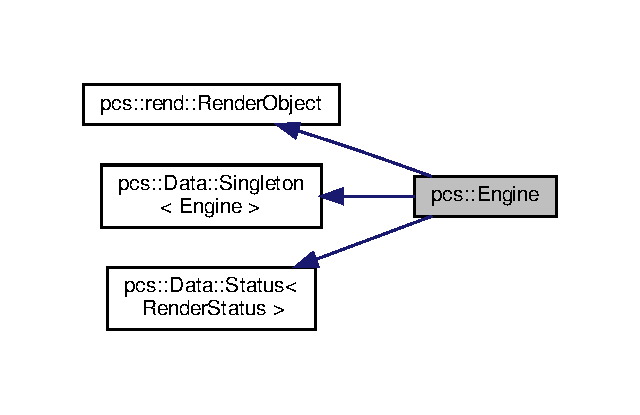
\includegraphics[width=307pt]{classpcs_1_1Engine__inherit__graph}
\end{center}
\end{figure}


Collaboration diagram for pcs\+:\+:Engine\+:\nopagebreak
\begin{figure}[H]
\begin{center}
\leavevmode
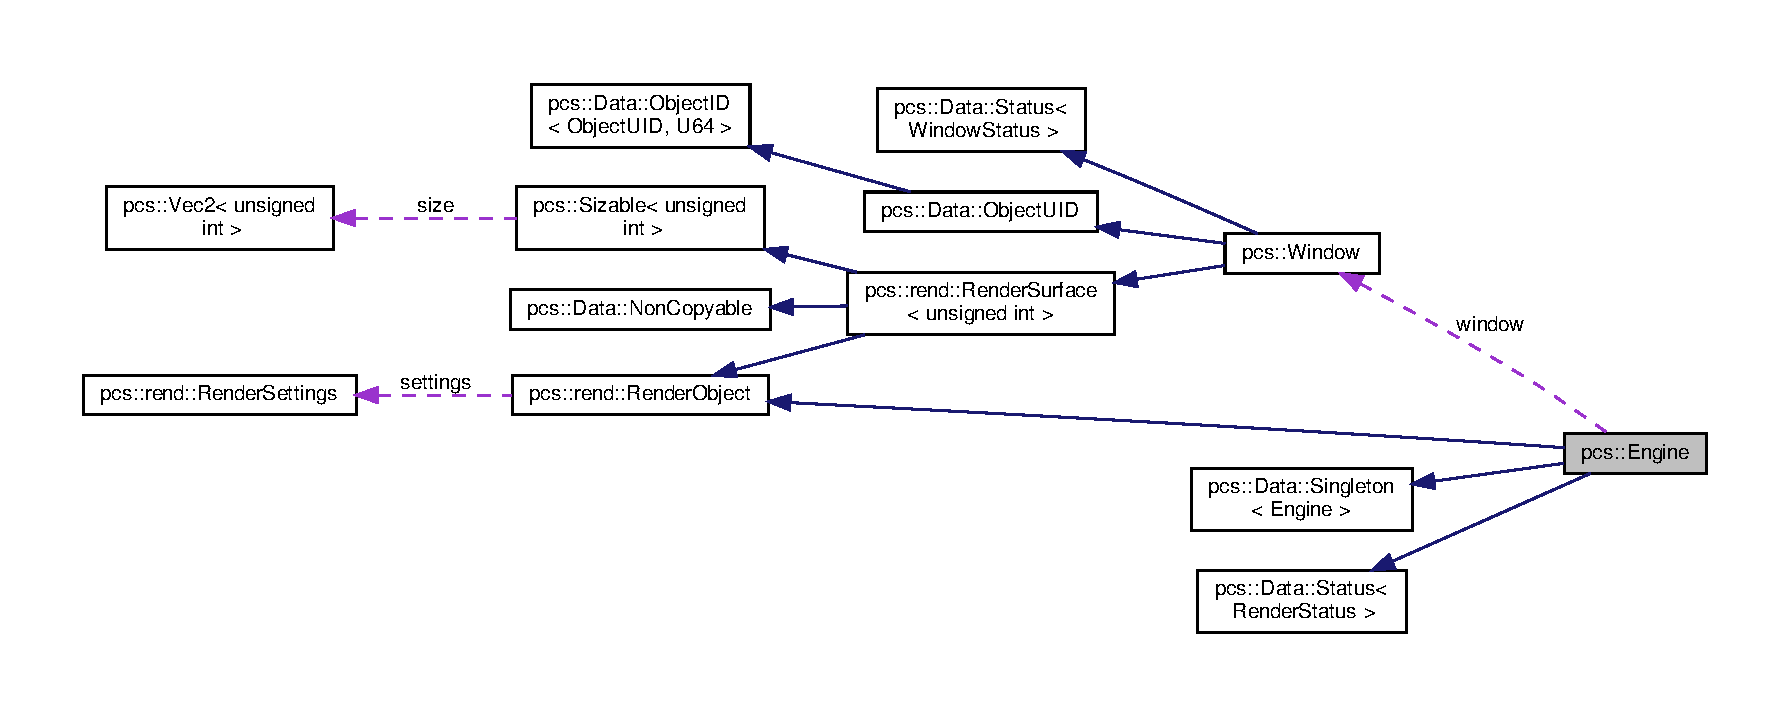
\includegraphics[width=350pt]{classpcs_1_1Engine__coll__graph}
\end{center}
\end{figure}
\subsection*{Public Member Functions}
\begin{DoxyCompactItemize}
\item 
\hyperlink{classpcs_1_1Engine_a73a5c3ce66c2c033835f19f95b67f3ea}{Engine} ()
\begin{DoxyCompactList}\small\item\em Constructs a new \hyperlink{classpcs_1_1Engine}{Engine} object. \end{DoxyCompactList}\item 
\hyperlink{classpcs_1_1Engine_aa6a523009abf3a61d9682a846c780207}{$\sim$\+Engine} ()
\begin{DoxyCompactList}\small\item\em Destroys the \hyperlink{classpcs_1_1Engine}{Engine} object. \end{DoxyCompactList}\item 
\hyperlink{namespacepcs_a979c2971659f1655c7ebe27752b8a9a0}{Render\+Status} \hyperlink{classpcs_1_1Engine_ad99225f71f2e1dd2b02bd99ad2c59ab3}{render\+Scene} (\hyperlink{classpcs_1_1Scene}{Scene} $\ast$scene) const
\begin{DoxyCompactList}\small\item\em Renders a given scene to the window. \end{DoxyCompactList}\item 
\hyperlink{classpcs_1_1Window}{Window} $\ast$ \hyperlink{classpcs_1_1Engine_a3bf8432ad5c397ea7bb3f95728fa9792}{get\+Window} ()
\begin{DoxyCompactList}\small\item\em Get the \hyperlink{classpcs_1_1Window}{Window} instance associated with this engine. \end{DoxyCompactList}\item 
void \hyperlink{classpcs_1_1Engine_ab43d2dd55c8519da49f92e7ccef042a8}{push\+Camera} (void $\ast$camera)
\begin{DoxyCompactList}\small\item\em Push a camera to the directory. \end{DoxyCompactList}\item 
std\+::vector$<$ void $\ast$ $>$ \& \hyperlink{classpcs_1_1Engine_a71059ef96479c7ca59901bfa0be2587a}{get\+Camera\+Directory} ()
\begin{DoxyCompactList}\small\item\em Get the \hyperlink{classpcs_1_1Camera}{Camera} Directory. \end{DoxyCompactList}\end{DoxyCompactItemize}
\subsection*{Private Attributes}
\begin{DoxyCompactItemize}
\item 
std\+::vector$<$ void $\ast$ $>$ \hyperlink{classpcs_1_1Engine_ad004e5859bca9815210a0f3786b83a02}{camera\+\_\+directory}
\item 
\hyperlink{classpcs_1_1Window}{Window} $\ast$ \hyperlink{classpcs_1_1Engine_a9d6dcbb93509389d86beb46ba33371a1}{window}
\begin{DoxyCompactList}\small\item\em \hyperlink{classpcs_1_1Window}{Window} on which to render to. \end{DoxyCompactList}\end{DoxyCompactItemize}
\subsection*{Additional Inherited Members}


\subsection{Detailed Description}
Handles rendering and holds the window instance. 

\subsection{Constructor \& Destructor Documentation}
\mbox{\Hypertarget{classpcs_1_1Engine_a73a5c3ce66c2c033835f19f95b67f3ea}\label{classpcs_1_1Engine_a73a5c3ce66c2c033835f19f95b67f3ea}} 
\index{pcs\+::\+Engine@{pcs\+::\+Engine}!Engine@{Engine}}
\index{Engine@{Engine}!pcs\+::\+Engine@{pcs\+::\+Engine}}
\subsubsection{\texorpdfstring{Engine()}{Engine()}}
{\footnotesize\ttfamily pcs\+::\+Engine\+::\+Engine (\begin{DoxyParamCaption}{ }\end{DoxyParamCaption})}



Constructs a new \hyperlink{classpcs_1_1Engine}{Engine} object. 

\mbox{\Hypertarget{classpcs_1_1Engine_aa6a523009abf3a61d9682a846c780207}\label{classpcs_1_1Engine_aa6a523009abf3a61d9682a846c780207}} 
\index{pcs\+::\+Engine@{pcs\+::\+Engine}!````~Engine@{$\sim$\+Engine}}
\index{````~Engine@{$\sim$\+Engine}!pcs\+::\+Engine@{pcs\+::\+Engine}}
\subsubsection{\texorpdfstring{$\sim$\+Engine()}{~Engine()}}
{\footnotesize\ttfamily pcs\+::\+Engine\+::$\sim$\+Engine (\begin{DoxyParamCaption}{ }\end{DoxyParamCaption})}



Destroys the \hyperlink{classpcs_1_1Engine}{Engine} object. 



\subsection{Member Function Documentation}
\mbox{\Hypertarget{classpcs_1_1Engine_a71059ef96479c7ca59901bfa0be2587a}\label{classpcs_1_1Engine_a71059ef96479c7ca59901bfa0be2587a}} 
\index{pcs\+::\+Engine@{pcs\+::\+Engine}!get\+Camera\+Directory@{get\+Camera\+Directory}}
\index{get\+Camera\+Directory@{get\+Camera\+Directory}!pcs\+::\+Engine@{pcs\+::\+Engine}}
\subsubsection{\texorpdfstring{get\+Camera\+Directory()}{getCameraDirectory()}}
{\footnotesize\ttfamily std\+::vector$<$void$\ast$$>$\& pcs\+::\+Engine\+::get\+Camera\+Directory (\begin{DoxyParamCaption}{ }\end{DoxyParamCaption})\hspace{0.3cm}{\ttfamily [inline]}}



Get the \hyperlink{classpcs_1_1Camera}{Camera} Directory. 

\begin{DoxyReturn}{Returns}
std\+::vector$<$void$\ast$$>$\& \hyperlink{classpcs_1_1Camera}{Camera} Directory list 
\end{DoxyReturn}
\mbox{\Hypertarget{classpcs_1_1Engine_a3bf8432ad5c397ea7bb3f95728fa9792}\label{classpcs_1_1Engine_a3bf8432ad5c397ea7bb3f95728fa9792}} 
\index{pcs\+::\+Engine@{pcs\+::\+Engine}!get\+Window@{get\+Window}}
\index{get\+Window@{get\+Window}!pcs\+::\+Engine@{pcs\+::\+Engine}}
\subsubsection{\texorpdfstring{get\+Window()}{getWindow()}}
{\footnotesize\ttfamily \hyperlink{classpcs_1_1Window}{Window}$\ast$ pcs\+::\+Engine\+::get\+Window (\begin{DoxyParamCaption}{ }\end{DoxyParamCaption})\hspace{0.3cm}{\ttfamily [inline]}}



Get the \hyperlink{classpcs_1_1Window}{Window} instance associated with this engine. 

\begin{DoxyReturn}{Returns}
Window$\ast$ Pointer to a window instance 
\end{DoxyReturn}
\mbox{\Hypertarget{classpcs_1_1Engine_ab43d2dd55c8519da49f92e7ccef042a8}\label{classpcs_1_1Engine_ab43d2dd55c8519da49f92e7ccef042a8}} 
\index{pcs\+::\+Engine@{pcs\+::\+Engine}!push\+Camera@{push\+Camera}}
\index{push\+Camera@{push\+Camera}!pcs\+::\+Engine@{pcs\+::\+Engine}}
\subsubsection{\texorpdfstring{push\+Camera()}{pushCamera()}}
{\footnotesize\ttfamily void pcs\+::\+Engine\+::push\+Camera (\begin{DoxyParamCaption}\item[{void $\ast$}]{camera }\end{DoxyParamCaption})\hspace{0.3cm}{\ttfamily [inline]}}



Push a camera to the directory. 


\begin{DoxyParams}{Parameters}
{\em camera} & \hyperlink{classpcs_1_1Camera}{Camera} instance to register \\
\hline
\end{DoxyParams}
\mbox{\Hypertarget{classpcs_1_1Engine_ad99225f71f2e1dd2b02bd99ad2c59ab3}\label{classpcs_1_1Engine_ad99225f71f2e1dd2b02bd99ad2c59ab3}} 
\index{pcs\+::\+Engine@{pcs\+::\+Engine}!render\+Scene@{render\+Scene}}
\index{render\+Scene@{render\+Scene}!pcs\+::\+Engine@{pcs\+::\+Engine}}
\subsubsection{\texorpdfstring{render\+Scene()}{renderScene()}}
{\footnotesize\ttfamily \hyperlink{namespacepcs_a979c2971659f1655c7ebe27752b8a9a0}{Render\+Status} pcs\+::\+Engine\+::render\+Scene (\begin{DoxyParamCaption}\item[{\hyperlink{classpcs_1_1Scene}{Scene} $\ast$}]{scene }\end{DoxyParamCaption}) const}



Renders a given scene to the window. 


\begin{DoxyParams}{Parameters}
{\em scene} & Pointer to a scene to render \\
\hline
\end{DoxyParams}
\begin{DoxyReturn}{Returns}
Render\+Status Status of the render 
\end{DoxyReturn}


\subsection{Member Data Documentation}
\mbox{\Hypertarget{classpcs_1_1Engine_ad004e5859bca9815210a0f3786b83a02}\label{classpcs_1_1Engine_ad004e5859bca9815210a0f3786b83a02}} 
\index{pcs\+::\+Engine@{pcs\+::\+Engine}!camera\+\_\+directory@{camera\+\_\+directory}}
\index{camera\+\_\+directory@{camera\+\_\+directory}!pcs\+::\+Engine@{pcs\+::\+Engine}}
\subsubsection{\texorpdfstring{camera\+\_\+directory}{camera\_directory}}
{\footnotesize\ttfamily std\+::vector$<$void$\ast$$>$ pcs\+::\+Engine\+::camera\+\_\+directory\hspace{0.3cm}{\ttfamily [private]}}

List of independent-\/typed pointers which each point to a camera associated with this engine. \mbox{\Hypertarget{classpcs_1_1Engine_a9d6dcbb93509389d86beb46ba33371a1}\label{classpcs_1_1Engine_a9d6dcbb93509389d86beb46ba33371a1}} 
\index{pcs\+::\+Engine@{pcs\+::\+Engine}!window@{window}}
\index{window@{window}!pcs\+::\+Engine@{pcs\+::\+Engine}}
\subsubsection{\texorpdfstring{window}{window}}
{\footnotesize\ttfamily \hyperlink{classpcs_1_1Window}{Window}$\ast$ pcs\+::\+Engine\+::window\hspace{0.3cm}{\ttfamily [private]}}



\hyperlink{classpcs_1_1Window}{Window} on which to render to. 



The documentation for this class was generated from the following files\+:\begin{DoxyCompactItemize}
\item 
include/\+Perceus/\+Core/\hyperlink{Engine_8h}{Engine.\+h}\item 
src/\+Core/\hyperlink{Engine_8cpp}{Engine.\+cpp}\end{DoxyCompactItemize}

\hypertarget{classpcs_1_1Event}{}\section{pcs\+:\+:Event Class Reference}
\label{classpcs_1_1Event}\index{pcs\+::\+Event@{pcs\+::\+Event}}


{\ttfamily \#include $<$Event.\+h$>$}



Inheritance diagram for pcs\+:\+:Event\+:\nopagebreak
\begin{figure}[H]
\begin{center}
\leavevmode
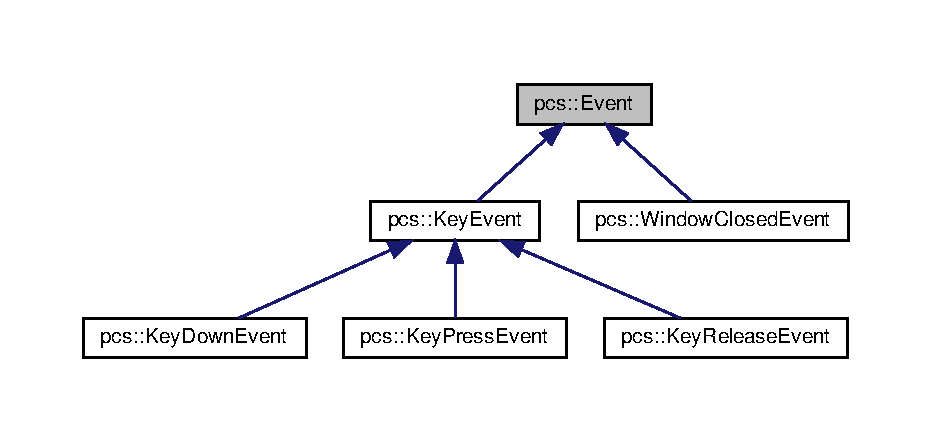
\includegraphics[width=350pt]{classpcs_1_1Event__inherit__graph}
\end{center}
\end{figure}
\subsection*{Public Member Functions}
\begin{DoxyCompactItemize}
\item 
virtual int \hyperlink{classpcs_1_1Event_a1cdcf7b0410496912c19417f72caed48}{get\+Category\+Flags} () const =0
\item 
virtual const char $\ast$ \hyperlink{classpcs_1_1Event_a066245823d5a005204574bccd544d8dd}{get\+Category} () const =0
\item 
virtual \hyperlink{namespacepcs_a12954f53e3d7d6a8765fd723e1ce8db4}{Event\+Type} \hyperlink{classpcs_1_1Event_a7ea17b26f979770e7809af854efe0f57}{get\+Type} () const =0
\item 
virtual const char $\ast$ \hyperlink{classpcs_1_1Event_a08392dd589a27532532b61103af6f291}{get\+Name} () const =0
\item 
bool \hyperlink{classpcs_1_1Event_ad3d636ba00a11cab150c2fdad81acc93}{in\+Category} (\hyperlink{namespacepcs_a3538ef524602fc09ddb40acc72480c60}{Event\+Category} category)
\end{DoxyCompactItemize}
\subsection*{Protected Attributes}
\begin{DoxyCompactItemize}
\item 
bool \hyperlink{classpcs_1_1Event_a24acdd6f068d4b4bbc61cab76f59e0ed}{handled} = false
\end{DoxyCompactItemize}


\subsection{Member Function Documentation}
\mbox{\Hypertarget{classpcs_1_1Event_a066245823d5a005204574bccd544d8dd}\label{classpcs_1_1Event_a066245823d5a005204574bccd544d8dd}} 
\index{pcs\+::\+Event@{pcs\+::\+Event}!get\+Category@{get\+Category}}
\index{get\+Category@{get\+Category}!pcs\+::\+Event@{pcs\+::\+Event}}
\subsubsection{\texorpdfstring{get\+Category()}{getCategory()}}
{\footnotesize\ttfamily virtual const char$\ast$ pcs\+::\+Event\+::get\+Category (\begin{DoxyParamCaption}{ }\end{DoxyParamCaption}) const\hspace{0.3cm}{\ttfamily [pure virtual]}}

\mbox{\Hypertarget{classpcs_1_1Event_a1cdcf7b0410496912c19417f72caed48}\label{classpcs_1_1Event_a1cdcf7b0410496912c19417f72caed48}} 
\index{pcs\+::\+Event@{pcs\+::\+Event}!get\+Category\+Flags@{get\+Category\+Flags}}
\index{get\+Category\+Flags@{get\+Category\+Flags}!pcs\+::\+Event@{pcs\+::\+Event}}
\subsubsection{\texorpdfstring{get\+Category\+Flags()}{getCategoryFlags()}}
{\footnotesize\ttfamily virtual int pcs\+::\+Event\+::get\+Category\+Flags (\begin{DoxyParamCaption}{ }\end{DoxyParamCaption}) const\hspace{0.3cm}{\ttfamily [pure virtual]}}

\mbox{\Hypertarget{classpcs_1_1Event_a08392dd589a27532532b61103af6f291}\label{classpcs_1_1Event_a08392dd589a27532532b61103af6f291}} 
\index{pcs\+::\+Event@{pcs\+::\+Event}!get\+Name@{get\+Name}}
\index{get\+Name@{get\+Name}!pcs\+::\+Event@{pcs\+::\+Event}}
\subsubsection{\texorpdfstring{get\+Name()}{getName()}}
{\footnotesize\ttfamily virtual const char$\ast$ pcs\+::\+Event\+::get\+Name (\begin{DoxyParamCaption}{ }\end{DoxyParamCaption}) const\hspace{0.3cm}{\ttfamily [pure virtual]}}

\mbox{\Hypertarget{classpcs_1_1Event_a7ea17b26f979770e7809af854efe0f57}\label{classpcs_1_1Event_a7ea17b26f979770e7809af854efe0f57}} 
\index{pcs\+::\+Event@{pcs\+::\+Event}!get\+Type@{get\+Type}}
\index{get\+Type@{get\+Type}!pcs\+::\+Event@{pcs\+::\+Event}}
\subsubsection{\texorpdfstring{get\+Type()}{getType()}}
{\footnotesize\ttfamily virtual \hyperlink{namespacepcs_a12954f53e3d7d6a8765fd723e1ce8db4}{Event\+Type} pcs\+::\+Event\+::get\+Type (\begin{DoxyParamCaption}{ }\end{DoxyParamCaption}) const\hspace{0.3cm}{\ttfamily [pure virtual]}}

\mbox{\Hypertarget{classpcs_1_1Event_ad3d636ba00a11cab150c2fdad81acc93}\label{classpcs_1_1Event_ad3d636ba00a11cab150c2fdad81acc93}} 
\index{pcs\+::\+Event@{pcs\+::\+Event}!in\+Category@{in\+Category}}
\index{in\+Category@{in\+Category}!pcs\+::\+Event@{pcs\+::\+Event}}
\subsubsection{\texorpdfstring{in\+Category()}{inCategory()}}
{\footnotesize\ttfamily bool pcs\+::\+Event\+::in\+Category (\begin{DoxyParamCaption}\item[{\hyperlink{namespacepcs_a3538ef524602fc09ddb40acc72480c60}{Event\+Category}}]{category }\end{DoxyParamCaption})\hspace{0.3cm}{\ttfamily [inline]}}



\subsection{Member Data Documentation}
\mbox{\Hypertarget{classpcs_1_1Event_a24acdd6f068d4b4bbc61cab76f59e0ed}\label{classpcs_1_1Event_a24acdd6f068d4b4bbc61cab76f59e0ed}} 
\index{pcs\+::\+Event@{pcs\+::\+Event}!handled@{handled}}
\index{handled@{handled}!pcs\+::\+Event@{pcs\+::\+Event}}
\subsubsection{\texorpdfstring{handled}{handled}}
{\footnotesize\ttfamily bool pcs\+::\+Event\+::handled = false\hspace{0.3cm}{\ttfamily [protected]}}



The documentation for this class was generated from the following file\+:\begin{DoxyCompactItemize}
\item 
include/\+Perceus/\+Core/\+Graphics/\+Rendering/\+Events/\hyperlink{Event_8h}{Event.\+h}\end{DoxyCompactItemize}

\hypertarget{classpcs_1_1EventHandler}{}\section{pcs\+:\+:Event\+Handler Class Reference}
\label{classpcs_1_1EventHandler}\index{pcs\+::\+Event\+Handler@{pcs\+::\+Event\+Handler}}


{\ttfamily \#include $<$Event\+Handler.\+h$>$}



Inheritance diagram for pcs\+:\+:Event\+Handler\+:\nopagebreak
\begin{figure}[H]
\begin{center}
\leavevmode
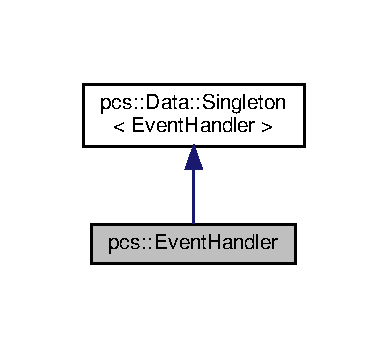
\includegraphics[width=186pt]{classpcs_1_1EventHandler__inherit__graph}
\end{center}
\end{figure}


Collaboration diagram for pcs\+:\+:Event\+Handler\+:\nopagebreak
\begin{figure}[H]
\begin{center}
\leavevmode
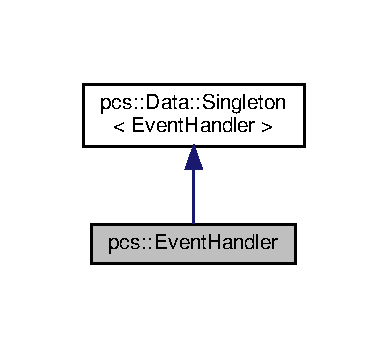
\includegraphics[width=186pt]{classpcs_1_1EventHandler__coll__graph}
\end{center}
\end{figure}
\subsection*{Public Member Functions}
\begin{DoxyCompactItemize}
\item 
\hyperlink{classpcs_1_1EventHandler_af980c02cecb98a61be2d23dcdbb525c4}{Event\+Handler} ()
\item 
\hyperlink{classpcs_1_1Event}{Event} $\ast$ \hyperlink{classpcs_1_1EventHandler_ac55d94bdc1d32947725e63ca0d5e93cb}{get\+Event} ()
\item 
{\footnotesize template$<$typename T , typename... Args$>$ }\\void \hyperlink{classpcs_1_1EventHandler_aa149c95e48d820d7c61f70c98b158e6b}{push\+Event} (Args... args)
\end{DoxyCompactItemize}
\subsection*{Private Member Functions}
\begin{DoxyCompactItemize}
\item 
void \hyperlink{classpcs_1_1EventHandler_a91240cdab030a6d37b9c9799305a9e8a}{clear\+Events} ()
\end{DoxyCompactItemize}
\subsection*{Private Attributes}
\begin{DoxyCompactItemize}
\item 
unsigned int \hyperlink{classpcs_1_1EventHandler_a31eccb3a5277a000785059cb34b31fd1}{inc} = 0
\item 
std\+::vector$<$ \hyperlink{classpcs_1_1Event}{Event} $\ast$ $>$ \hyperlink{classpcs_1_1EventHandler_a05bd1c27d4ee1082c31fcaf767a43939}{events}
\end{DoxyCompactItemize}
\subsection*{Friends}
\begin{DoxyCompactItemize}
\item 
class \hyperlink{classpcs_1_1EventHandler_a3e1914489e4bed4f9f23cdeab34a43dc}{Engine}
\end{DoxyCompactItemize}
\subsection*{Additional Inherited Members}


\subsection{Constructor \& Destructor Documentation}
\mbox{\Hypertarget{classpcs_1_1EventHandler_af980c02cecb98a61be2d23dcdbb525c4}\label{classpcs_1_1EventHandler_af980c02cecb98a61be2d23dcdbb525c4}} 
\index{pcs\+::\+Event\+Handler@{pcs\+::\+Event\+Handler}!Event\+Handler@{Event\+Handler}}
\index{Event\+Handler@{Event\+Handler}!pcs\+::\+Event\+Handler@{pcs\+::\+Event\+Handler}}
\subsubsection{\texorpdfstring{Event\+Handler()}{EventHandler()}}
{\footnotesize\ttfamily pcs\+::\+Event\+Handler\+::\+Event\+Handler (\begin{DoxyParamCaption}{ }\end{DoxyParamCaption})}



\subsection{Member Function Documentation}
\mbox{\Hypertarget{classpcs_1_1EventHandler_a91240cdab030a6d37b9c9799305a9e8a}\label{classpcs_1_1EventHandler_a91240cdab030a6d37b9c9799305a9e8a}} 
\index{pcs\+::\+Event\+Handler@{pcs\+::\+Event\+Handler}!clear\+Events@{clear\+Events}}
\index{clear\+Events@{clear\+Events}!pcs\+::\+Event\+Handler@{pcs\+::\+Event\+Handler}}
\subsubsection{\texorpdfstring{clear\+Events()}{clearEvents()}}
{\footnotesize\ttfamily void pcs\+::\+Event\+Handler\+::clear\+Events (\begin{DoxyParamCaption}{ }\end{DoxyParamCaption})\hspace{0.3cm}{\ttfamily [private]}}

\mbox{\Hypertarget{classpcs_1_1EventHandler_ac55d94bdc1d32947725e63ca0d5e93cb}\label{classpcs_1_1EventHandler_ac55d94bdc1d32947725e63ca0d5e93cb}} 
\index{pcs\+::\+Event\+Handler@{pcs\+::\+Event\+Handler}!get\+Event@{get\+Event}}
\index{get\+Event@{get\+Event}!pcs\+::\+Event\+Handler@{pcs\+::\+Event\+Handler}}
\subsubsection{\texorpdfstring{get\+Event()}{getEvent()}}
{\footnotesize\ttfamily \hyperlink{classpcs_1_1Event}{Event} $\ast$ pcs\+::\+Event\+Handler\+::get\+Event (\begin{DoxyParamCaption}{ }\end{DoxyParamCaption})}

\mbox{\Hypertarget{classpcs_1_1EventHandler_aa149c95e48d820d7c61f70c98b158e6b}\label{classpcs_1_1EventHandler_aa149c95e48d820d7c61f70c98b158e6b}} 
\index{pcs\+::\+Event\+Handler@{pcs\+::\+Event\+Handler}!push\+Event@{push\+Event}}
\index{push\+Event@{push\+Event}!pcs\+::\+Event\+Handler@{pcs\+::\+Event\+Handler}}
\subsubsection{\texorpdfstring{push\+Event()}{pushEvent()}}
{\footnotesize\ttfamily template$<$typename T , typename... Args$>$ \\
void pcs\+::\+Event\+Handler\+::push\+Event (\begin{DoxyParamCaption}\item[{Args...}]{args }\end{DoxyParamCaption})\hspace{0.3cm}{\ttfamily [inline]}}



\subsection{Friends And Related Function Documentation}
\mbox{\Hypertarget{classpcs_1_1EventHandler_a3e1914489e4bed4f9f23cdeab34a43dc}\label{classpcs_1_1EventHandler_a3e1914489e4bed4f9f23cdeab34a43dc}} 
\index{pcs\+::\+Event\+Handler@{pcs\+::\+Event\+Handler}!Engine@{Engine}}
\index{Engine@{Engine}!pcs\+::\+Event\+Handler@{pcs\+::\+Event\+Handler}}
\subsubsection{\texorpdfstring{Engine}{Engine}}
{\footnotesize\ttfamily friend class \hyperlink{classpcs_1_1Engine}{Engine}\hspace{0.3cm}{\ttfamily [friend]}}



\subsection{Member Data Documentation}
\mbox{\Hypertarget{classpcs_1_1EventHandler_a05bd1c27d4ee1082c31fcaf767a43939}\label{classpcs_1_1EventHandler_a05bd1c27d4ee1082c31fcaf767a43939}} 
\index{pcs\+::\+Event\+Handler@{pcs\+::\+Event\+Handler}!events@{events}}
\index{events@{events}!pcs\+::\+Event\+Handler@{pcs\+::\+Event\+Handler}}
\subsubsection{\texorpdfstring{events}{events}}
{\footnotesize\ttfamily std\+::vector$<$\hyperlink{classpcs_1_1Event}{Event}$\ast$$>$ pcs\+::\+Event\+Handler\+::events\hspace{0.3cm}{\ttfamily [private]}}

\mbox{\Hypertarget{classpcs_1_1EventHandler_a31eccb3a5277a000785059cb34b31fd1}\label{classpcs_1_1EventHandler_a31eccb3a5277a000785059cb34b31fd1}} 
\index{pcs\+::\+Event\+Handler@{pcs\+::\+Event\+Handler}!inc@{inc}}
\index{inc@{inc}!pcs\+::\+Event\+Handler@{pcs\+::\+Event\+Handler}}
\subsubsection{\texorpdfstring{inc}{inc}}
{\footnotesize\ttfamily unsigned int pcs\+::\+Event\+Handler\+::inc = 0\hspace{0.3cm}{\ttfamily [private]}}



The documentation for this class was generated from the following files\+:\begin{DoxyCompactItemize}
\item 
include/\+Perceus/\+Core/\+Graphics/\+Rendering/\+Events/\hyperlink{EventHandler_8h}{Event\+Handler.\+h}\item 
src/\+Core/\+Graphics/\+Rendering/\+Events/\hyperlink{EventHandler_8cpp}{Event\+Handler.\+cpp}\end{DoxyCompactItemize}

\hypertarget{classpcs_1_1File}{}\section{pcs\+:\+:File Class Reference}
\label{classpcs_1_1File}\index{pcs\+::\+File@{pcs\+::\+File}}


{\ttfamily \#include $<$File.\+h$>$}



Inheritance diagram for pcs\+:\+:File\+:\nopagebreak
\begin{figure}[H]
\begin{center}
\leavevmode
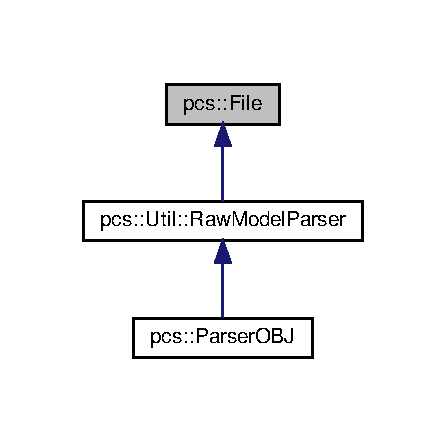
\includegraphics[width=214pt]{classpcs_1_1File__inherit__graph}
\end{center}
\end{figure}
\subsection*{Public Member Functions}
\begin{DoxyCompactItemize}
\item 
\hyperlink{classpcs_1_1File_a26d8a7d8ce42c0217b42845eee341c56}{File} (const char $\ast$location)
\item 
{\footnotesize template$<$typename... Args$>$ }\\const char $\ast$ \hyperlink{classpcs_1_1File_a63b32c52dd5d6d3fa51a0178eae44ab4}{get\+File\+Contents} (void($\ast$f)(const char $\ast$, Args...)=nullptr, Args... args) const
\end{DoxyCompactItemize}
\subsection*{Protected Attributes}
\begin{DoxyCompactItemize}
\item 
const char $\ast$ \hyperlink{classpcs_1_1File_aba44c03eedf48cbe021f05680bfe6614}{file\+Location}
\end{DoxyCompactItemize}


\subsection{Constructor \& Destructor Documentation}
\mbox{\Hypertarget{classpcs_1_1File_a26d8a7d8ce42c0217b42845eee341c56}\label{classpcs_1_1File_a26d8a7d8ce42c0217b42845eee341c56}} 
\index{pcs\+::\+File@{pcs\+::\+File}!File@{File}}
\index{File@{File}!pcs\+::\+File@{pcs\+::\+File}}
\subsubsection{\texorpdfstring{File()}{File()}}
{\footnotesize\ttfamily pcs\+::\+File\+::\+File (\begin{DoxyParamCaption}\item[{const char $\ast$}]{location }\end{DoxyParamCaption})}



\subsection{Member Function Documentation}
\mbox{\Hypertarget{classpcs_1_1File_a63b32c52dd5d6d3fa51a0178eae44ab4}\label{classpcs_1_1File_a63b32c52dd5d6d3fa51a0178eae44ab4}} 
\index{pcs\+::\+File@{pcs\+::\+File}!get\+File\+Contents@{get\+File\+Contents}}
\index{get\+File\+Contents@{get\+File\+Contents}!pcs\+::\+File@{pcs\+::\+File}}
\subsubsection{\texorpdfstring{get\+File\+Contents()}{getFileContents()}}
{\footnotesize\ttfamily template$<$typename... Args$>$ \\
const char$\ast$ pcs\+::\+File\+::get\+File\+Contents (\begin{DoxyParamCaption}\item[{void($\ast$)(const char $\ast$, Args...)}]{f = {\ttfamily nullptr},  }\item[{Args...}]{args }\end{DoxyParamCaption}) const\hspace{0.3cm}{\ttfamily [inline]}}



\subsection{Member Data Documentation}
\mbox{\Hypertarget{classpcs_1_1File_aba44c03eedf48cbe021f05680bfe6614}\label{classpcs_1_1File_aba44c03eedf48cbe021f05680bfe6614}} 
\index{pcs\+::\+File@{pcs\+::\+File}!file\+Location@{file\+Location}}
\index{file\+Location@{file\+Location}!pcs\+::\+File@{pcs\+::\+File}}
\subsubsection{\texorpdfstring{file\+Location}{fileLocation}}
{\footnotesize\ttfamily const char$\ast$ pcs\+::\+File\+::file\+Location\hspace{0.3cm}{\ttfamily [protected]}}



The documentation for this class was generated from the following files\+:\begin{DoxyCompactItemize}
\item 
include/\+Perceus/\+Util/\hyperlink{File_8h}{File.\+h}\item 
src/\+Util/\hyperlink{File_8cpp}{File.\+cpp}\end{DoxyCompactItemize}

\hypertarget{classpcs_1_1ForwardRenderer}{}\section{pcs\+:\+:Forward\+Renderer Class Reference}
\label{classpcs_1_1ForwardRenderer}\index{pcs\+::\+Forward\+Renderer@{pcs\+::\+Forward\+Renderer}}


{\ttfamily \#include $<$Forward\+Renderer.\+h$>$}



Inheritance diagram for pcs\+:\+:Forward\+Renderer\+:\nopagebreak
\begin{figure}[H]
\begin{center}
\leavevmode
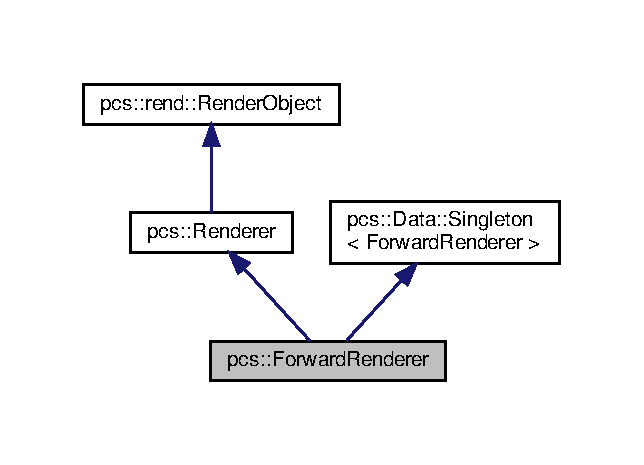
\includegraphics[width=309pt]{classpcs_1_1ForwardRenderer__inherit__graph}
\end{center}
\end{figure}


Collaboration diagram for pcs\+:\+:Forward\+Renderer\+:\nopagebreak
\begin{figure}[H]
\begin{center}
\leavevmode
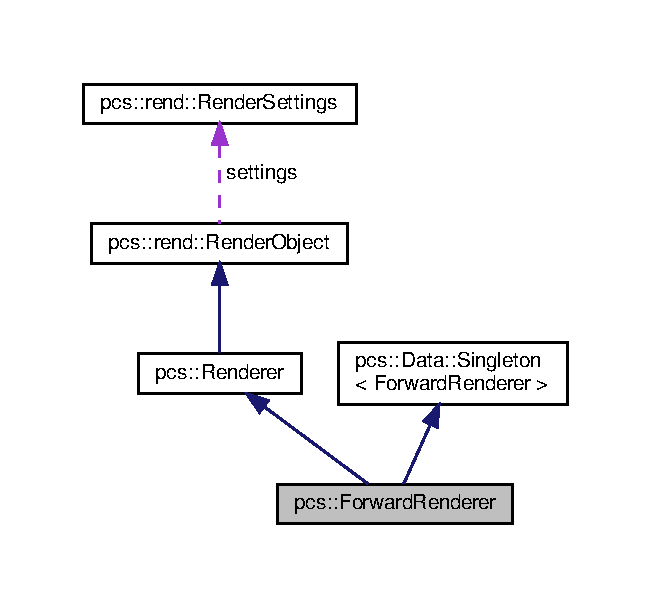
\includegraphics[width=313pt]{classpcs_1_1ForwardRenderer__coll__graph}
\end{center}
\end{figure}
\subsection*{Public Member Functions}
\begin{DoxyCompactItemize}
\item 
int \hyperlink{classpcs_1_1ForwardRenderer_a75527d1b400625fc9b33cddaff76bb33}{render} (\hyperlink{classpcs_1_1RawModel}{Raw\+Model} $\ast$raw\+Model, \hyperlink{classpcs_1_1ShaderProgram}{Shader\+Program} $\ast$shader, \hyperlink{classpcs_1_1Camera}{Camera} $\ast$camera, unsigned int count=1) const
\end{DoxyCompactItemize}
\subsection*{Additional Inherited Members}


\subsection{Member Function Documentation}
\mbox{\Hypertarget{classpcs_1_1ForwardRenderer_a75527d1b400625fc9b33cddaff76bb33}\label{classpcs_1_1ForwardRenderer_a75527d1b400625fc9b33cddaff76bb33}} 
\index{pcs\+::\+Forward\+Renderer@{pcs\+::\+Forward\+Renderer}!render@{render}}
\index{render@{render}!pcs\+::\+Forward\+Renderer@{pcs\+::\+Forward\+Renderer}}
\subsubsection{\texorpdfstring{render()}{render()}}
{\footnotesize\ttfamily int pcs\+::\+Forward\+Renderer\+::render (\begin{DoxyParamCaption}\item[{\hyperlink{classpcs_1_1RawModel}{Raw\+Model} $\ast$}]{raw\+Model,  }\item[{\hyperlink{classpcs_1_1ShaderProgram}{Shader\+Program} $\ast$}]{shader,  }\item[{\hyperlink{classpcs_1_1Camera}{Camera} $\ast$}]{camera,  }\item[{unsigned int}]{count = {\ttfamily 1} }\end{DoxyParamCaption}) const\hspace{0.3cm}{\ttfamily [virtual]}}



Implements \hyperlink{classpcs_1_1Renderer_aba6bdcf38357cdfea898e0f7b3cb1757}{pcs\+::\+Renderer}.



The documentation for this class was generated from the following files\+:\begin{DoxyCompactItemize}
\item 
include/\+Perceus/\+Core/\+Graphics/\+Rendering/\hyperlink{ForwardRenderer_8h}{Forward\+Renderer.\+h}\item 
src/\+Core/\+Graphics/\+Rendering/\hyperlink{ForwardRenderer_8cpp}{Forward\+Renderer.\+cpp}\end{DoxyCompactItemize}

\hypertarget{classpcs_1_1KeyDownEvent}{}\section{pcs\+:\+:Key\+Down\+Event Class Reference}
\label{classpcs_1_1KeyDownEvent}\index{pcs\+::\+Key\+Down\+Event@{pcs\+::\+Key\+Down\+Event}}


{\ttfamily \#include $<$Keyboard\+Events.\+h$>$}



Inheritance diagram for pcs\+:\+:Key\+Down\+Event\+:\nopagebreak
\begin{figure}[H]
\begin{center}
\leavevmode
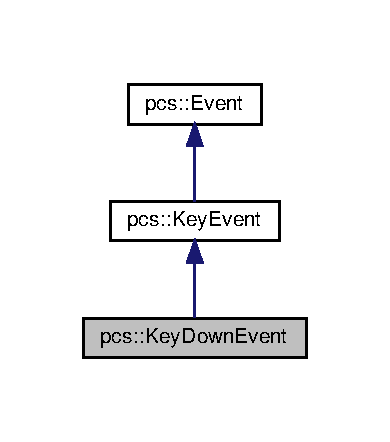
\includegraphics[width=187pt]{classpcs_1_1KeyDownEvent__inherit__graph}
\end{center}
\end{figure}


Collaboration diagram for pcs\+:\+:Key\+Down\+Event\+:\nopagebreak
\begin{figure}[H]
\begin{center}
\leavevmode
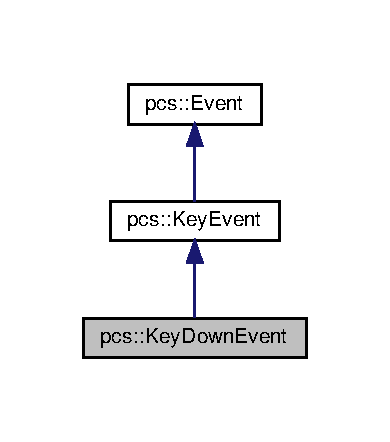
\includegraphics[width=187pt]{classpcs_1_1KeyDownEvent__coll__graph}
\end{center}
\end{figure}
\subsection*{Public Member Functions}
\begin{DoxyCompactItemize}
\item 
\hyperlink{classpcs_1_1KeyDownEvent_a66a843037aace9bed5e3be68b2eab56c}{Key\+Down\+Event} (const char c)
\item 
\hyperlink{classpcs_1_1KeyDownEvent_ae2f1f9e6fb979f79c1f97ca16226fbab}{E\+V\+E\+N\+T\+\_\+\+T\+Y\+PE} (\hyperlink{namespacepcs_a12954f53e3d7d6a8765fd723e1ce8db4acfd07bf1effd88bca04a12a087777354}{Key\+Down})
\end{DoxyCompactItemize}
\subsection*{Additional Inherited Members}


\subsection{Constructor \& Destructor Documentation}
\mbox{\Hypertarget{classpcs_1_1KeyDownEvent_a66a843037aace9bed5e3be68b2eab56c}\label{classpcs_1_1KeyDownEvent_a66a843037aace9bed5e3be68b2eab56c}} 
\index{pcs\+::\+Key\+Down\+Event@{pcs\+::\+Key\+Down\+Event}!Key\+Down\+Event@{Key\+Down\+Event}}
\index{Key\+Down\+Event@{Key\+Down\+Event}!pcs\+::\+Key\+Down\+Event@{pcs\+::\+Key\+Down\+Event}}
\subsubsection{\texorpdfstring{Key\+Down\+Event()}{KeyDownEvent()}}
{\footnotesize\ttfamily pcs\+::\+Key\+Down\+Event\+::\+Key\+Down\+Event (\begin{DoxyParamCaption}\item[{const char}]{c }\end{DoxyParamCaption})\hspace{0.3cm}{\ttfamily [inline]}}



\subsection{Member Function Documentation}
\mbox{\Hypertarget{classpcs_1_1KeyDownEvent_ae2f1f9e6fb979f79c1f97ca16226fbab}\label{classpcs_1_1KeyDownEvent_ae2f1f9e6fb979f79c1f97ca16226fbab}} 
\index{pcs\+::\+Key\+Down\+Event@{pcs\+::\+Key\+Down\+Event}!E\+V\+E\+N\+T\+\_\+\+T\+Y\+PE@{E\+V\+E\+N\+T\+\_\+\+T\+Y\+PE}}
\index{E\+V\+E\+N\+T\+\_\+\+T\+Y\+PE@{E\+V\+E\+N\+T\+\_\+\+T\+Y\+PE}!pcs\+::\+Key\+Down\+Event@{pcs\+::\+Key\+Down\+Event}}
\subsubsection{\texorpdfstring{E\+V\+E\+N\+T\+\_\+\+T\+Y\+P\+E()}{EVENT\_TYPE()}}
{\footnotesize\ttfamily pcs\+::\+Key\+Down\+Event\+::\+E\+V\+E\+N\+T\+\_\+\+T\+Y\+PE (\begin{DoxyParamCaption}\item[{\hyperlink{namespacepcs_a12954f53e3d7d6a8765fd723e1ce8db4acfd07bf1effd88bca04a12a087777354}{Key\+Down}}]{ }\end{DoxyParamCaption})}



The documentation for this class was generated from the following file\+:\begin{DoxyCompactItemize}
\item 
include/\+Perceus/\+Core/\+Graphics/\+Rendering/\+Events/\hyperlink{KeyboardEvents_8h}{Keyboard\+Events.\+h}\end{DoxyCompactItemize}

\hypertarget{classpcs_1_1KeyEvent}{}\section{pcs\+:\+:Key\+Event Class Reference}
\label{classpcs_1_1KeyEvent}\index{pcs\+::\+Key\+Event@{pcs\+::\+Key\+Event}}


{\ttfamily \#include $<$Keyboard\+Events.\+h$>$}



Inheritance diagram for pcs\+:\+:Key\+Event\+:\nopagebreak
\begin{figure}[H]
\begin{center}
\leavevmode
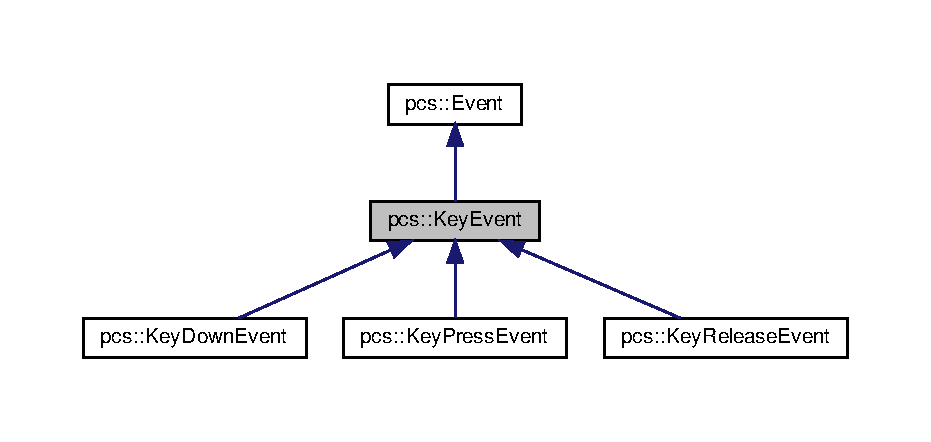
\includegraphics[width=350pt]{classpcs_1_1KeyEvent__inherit__graph}
\end{center}
\end{figure}


Collaboration diagram for pcs\+:\+:Key\+Event\+:\nopagebreak
\begin{figure}[H]
\begin{center}
\leavevmode
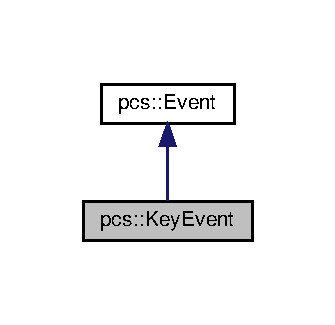
\includegraphics[width=161pt]{classpcs_1_1KeyEvent__coll__graph}
\end{center}
\end{figure}
\subsection*{Public Member Functions}
\begin{DoxyCompactItemize}
\item 
\hyperlink{classpcs_1_1KeyEvent_a238360a5576281a9d19a986a05cfd118}{Key\+Event} (const char c, \hyperlink{namespacepcs_a74212420ef246b051e11d561089ed547}{Key\+State} state)
\item 
\hyperlink{classpcs_1_1KeyEvent_a6b971ff54d31d691f6e5632a9863ba9b}{E\+V\+E\+N\+T\+\_\+\+C\+A\+T\+E\+G\+O\+RY} (\hyperlink{namespacepcs_a3538ef524602fc09ddb40acc72480c60a26cd4d5fcc5bb943efa4fd4ce0a69386}{Keyboard\+Event})
\item 
char \hyperlink{classpcs_1_1KeyEvent_ad1b80fa4d8b88aeb339973e27f1971dc}{get\+Key} () const
\end{DoxyCompactItemize}
\subsection*{Private Attributes}
\begin{DoxyCompactItemize}
\item 
char \hyperlink{classpcs_1_1KeyEvent_a583b56025e205125c2eae41f17e442e6}{ch}
\end{DoxyCompactItemize}
\subsection*{Static Private Attributes}
\begin{DoxyCompactItemize}
\item 
static unsigned int \hyperlink{classpcs_1_1KeyEvent_a4704e9758c494ee99e83226714b58412}{\+\_\+keycount} = 128
\item 
static int $\ast$ \hyperlink{classpcs_1_1KeyEvent_ade70c09116e673cc43d15721dea95965}{key\+\_\+states} = new int\mbox{[}\hyperlink{classpcs_1_1KeyEvent_a4704e9758c494ee99e83226714b58412}{Key\+Press\+Event\+::\+\_\+keycount}\mbox{]}
\end{DoxyCompactItemize}
\subsection*{Additional Inherited Members}


\subsection{Constructor \& Destructor Documentation}
\mbox{\Hypertarget{classpcs_1_1KeyEvent_a238360a5576281a9d19a986a05cfd118}\label{classpcs_1_1KeyEvent_a238360a5576281a9d19a986a05cfd118}} 
\index{pcs\+::\+Key\+Event@{pcs\+::\+Key\+Event}!Key\+Event@{Key\+Event}}
\index{Key\+Event@{Key\+Event}!pcs\+::\+Key\+Event@{pcs\+::\+Key\+Event}}
\subsubsection{\texorpdfstring{Key\+Event()}{KeyEvent()}}
{\footnotesize\ttfamily pcs\+::\+Key\+Event\+::\+Key\+Event (\begin{DoxyParamCaption}\item[{const char}]{c,  }\item[{\hyperlink{namespacepcs_a74212420ef246b051e11d561089ed547}{Key\+State}}]{state }\end{DoxyParamCaption})}



\subsection{Member Function Documentation}
\mbox{\Hypertarget{classpcs_1_1KeyEvent_a6b971ff54d31d691f6e5632a9863ba9b}\label{classpcs_1_1KeyEvent_a6b971ff54d31d691f6e5632a9863ba9b}} 
\index{pcs\+::\+Key\+Event@{pcs\+::\+Key\+Event}!E\+V\+E\+N\+T\+\_\+\+C\+A\+T\+E\+G\+O\+RY@{E\+V\+E\+N\+T\+\_\+\+C\+A\+T\+E\+G\+O\+RY}}
\index{E\+V\+E\+N\+T\+\_\+\+C\+A\+T\+E\+G\+O\+RY@{E\+V\+E\+N\+T\+\_\+\+C\+A\+T\+E\+G\+O\+RY}!pcs\+::\+Key\+Event@{pcs\+::\+Key\+Event}}
\subsubsection{\texorpdfstring{E\+V\+E\+N\+T\+\_\+\+C\+A\+T\+E\+G\+O\+R\+Y()}{EVENT\_CATEGORY()}}
{\footnotesize\ttfamily pcs\+::\+Key\+Event\+::\+E\+V\+E\+N\+T\+\_\+\+C\+A\+T\+E\+G\+O\+RY (\begin{DoxyParamCaption}\item[{\hyperlink{namespacepcs_a3538ef524602fc09ddb40acc72480c60a26cd4d5fcc5bb943efa4fd4ce0a69386}{Keyboard\+Event}}]{ }\end{DoxyParamCaption})}

\mbox{\Hypertarget{classpcs_1_1KeyEvent_ad1b80fa4d8b88aeb339973e27f1971dc}\label{classpcs_1_1KeyEvent_ad1b80fa4d8b88aeb339973e27f1971dc}} 
\index{pcs\+::\+Key\+Event@{pcs\+::\+Key\+Event}!get\+Key@{get\+Key}}
\index{get\+Key@{get\+Key}!pcs\+::\+Key\+Event@{pcs\+::\+Key\+Event}}
\subsubsection{\texorpdfstring{get\+Key()}{getKey()}}
{\footnotesize\ttfamily char pcs\+::\+Key\+Event\+::get\+Key (\begin{DoxyParamCaption}{ }\end{DoxyParamCaption}) const\hspace{0.3cm}{\ttfamily [inline]}}



\subsection{Member Data Documentation}
\mbox{\Hypertarget{classpcs_1_1KeyEvent_a4704e9758c494ee99e83226714b58412}\label{classpcs_1_1KeyEvent_a4704e9758c494ee99e83226714b58412}} 
\index{pcs\+::\+Key\+Event@{pcs\+::\+Key\+Event}!\+\_\+keycount@{\+\_\+keycount}}
\index{\+\_\+keycount@{\+\_\+keycount}!pcs\+::\+Key\+Event@{pcs\+::\+Key\+Event}}
\subsubsection{\texorpdfstring{\+\_\+keycount}{\_keycount}}
{\footnotesize\ttfamily unsigned int pcs\+::\+Key\+Event\+::\+\_\+keycount = 128\hspace{0.3cm}{\ttfamily [static]}, {\ttfamily [private]}}

\mbox{\Hypertarget{classpcs_1_1KeyEvent_a583b56025e205125c2eae41f17e442e6}\label{classpcs_1_1KeyEvent_a583b56025e205125c2eae41f17e442e6}} 
\index{pcs\+::\+Key\+Event@{pcs\+::\+Key\+Event}!ch@{ch}}
\index{ch@{ch}!pcs\+::\+Key\+Event@{pcs\+::\+Key\+Event}}
\subsubsection{\texorpdfstring{ch}{ch}}
{\footnotesize\ttfamily char pcs\+::\+Key\+Event\+::ch\hspace{0.3cm}{\ttfamily [private]}}

\mbox{\Hypertarget{classpcs_1_1KeyEvent_ade70c09116e673cc43d15721dea95965}\label{classpcs_1_1KeyEvent_ade70c09116e673cc43d15721dea95965}} 
\index{pcs\+::\+Key\+Event@{pcs\+::\+Key\+Event}!key\+\_\+states@{key\+\_\+states}}
\index{key\+\_\+states@{key\+\_\+states}!pcs\+::\+Key\+Event@{pcs\+::\+Key\+Event}}
\subsubsection{\texorpdfstring{key\+\_\+states}{key\_states}}
{\footnotesize\ttfamily int $\ast$ pcs\+::\+Key\+Event\+::key\+\_\+states = new int\mbox{[}\hyperlink{classpcs_1_1KeyEvent_a4704e9758c494ee99e83226714b58412}{Key\+Press\+Event\+::\+\_\+keycount}\mbox{]}\hspace{0.3cm}{\ttfamily [static]}, {\ttfamily [private]}}



The documentation for this class was generated from the following files\+:\begin{DoxyCompactItemize}
\item 
include/\+Perceus/\+Core/\+Graphics/\+Rendering/\+Events/\hyperlink{KeyboardEvents_8h}{Keyboard\+Events.\+h}\item 
src/\+Core/\+Graphics/\+Rendering/\+Events/\hyperlink{KeyboardEvents_8cpp}{Keyboard\+Events.\+cpp}\end{DoxyCompactItemize}

\hypertarget{classpcs_1_1KeyPressEvent}{}\section{pcs\+:\+:Key\+Press\+Event Class Reference}
\label{classpcs_1_1KeyPressEvent}\index{pcs\+::\+Key\+Press\+Event@{pcs\+::\+Key\+Press\+Event}}


{\ttfamily \#include $<$Keyboard\+Events.\+h$>$}



Inheritance diagram for pcs\+:\+:Key\+Press\+Event\+:\nopagebreak
\begin{figure}[H]
\begin{center}
\leavevmode
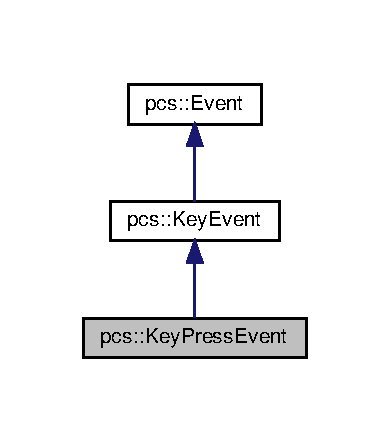
\includegraphics[width=187pt]{classpcs_1_1KeyPressEvent__inherit__graph}
\end{center}
\end{figure}


Collaboration diagram for pcs\+:\+:Key\+Press\+Event\+:\nopagebreak
\begin{figure}[H]
\begin{center}
\leavevmode
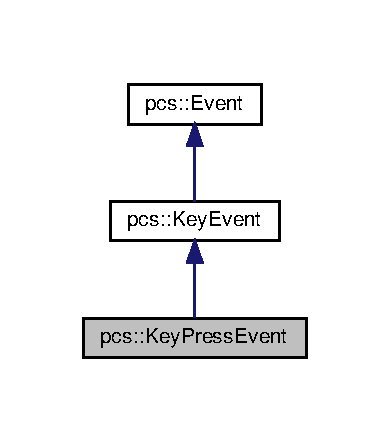
\includegraphics[width=187pt]{classpcs_1_1KeyPressEvent__coll__graph}
\end{center}
\end{figure}
\subsection*{Public Member Functions}
\begin{DoxyCompactItemize}
\item 
\hyperlink{classpcs_1_1KeyPressEvent_a6a9b7a9bb755f168047207c390df91c4}{Key\+Press\+Event} (const char c)
\item 
\hyperlink{classpcs_1_1KeyPressEvent_ad0ceb6d7e128aa6796f7907a0e4c7240}{E\+V\+E\+N\+T\+\_\+\+T\+Y\+PE} (\hyperlink{namespacepcs_a12954f53e3d7d6a8765fd723e1ce8db4a65a1aa093fcf3acd50b318f1942c02f5}{Key\+Press})
\end{DoxyCompactItemize}
\subsection*{Additional Inherited Members}


\subsection{Constructor \& Destructor Documentation}
\mbox{\Hypertarget{classpcs_1_1KeyPressEvent_a6a9b7a9bb755f168047207c390df91c4}\label{classpcs_1_1KeyPressEvent_a6a9b7a9bb755f168047207c390df91c4}} 
\index{pcs\+::\+Key\+Press\+Event@{pcs\+::\+Key\+Press\+Event}!Key\+Press\+Event@{Key\+Press\+Event}}
\index{Key\+Press\+Event@{Key\+Press\+Event}!pcs\+::\+Key\+Press\+Event@{pcs\+::\+Key\+Press\+Event}}
\subsubsection{\texorpdfstring{Key\+Press\+Event()}{KeyPressEvent()}}
{\footnotesize\ttfamily pcs\+::\+Key\+Press\+Event\+::\+Key\+Press\+Event (\begin{DoxyParamCaption}\item[{const char}]{c }\end{DoxyParamCaption})\hspace{0.3cm}{\ttfamily [inline]}}



\subsection{Member Function Documentation}
\mbox{\Hypertarget{classpcs_1_1KeyPressEvent_ad0ceb6d7e128aa6796f7907a0e4c7240}\label{classpcs_1_1KeyPressEvent_ad0ceb6d7e128aa6796f7907a0e4c7240}} 
\index{pcs\+::\+Key\+Press\+Event@{pcs\+::\+Key\+Press\+Event}!E\+V\+E\+N\+T\+\_\+\+T\+Y\+PE@{E\+V\+E\+N\+T\+\_\+\+T\+Y\+PE}}
\index{E\+V\+E\+N\+T\+\_\+\+T\+Y\+PE@{E\+V\+E\+N\+T\+\_\+\+T\+Y\+PE}!pcs\+::\+Key\+Press\+Event@{pcs\+::\+Key\+Press\+Event}}
\subsubsection{\texorpdfstring{E\+V\+E\+N\+T\+\_\+\+T\+Y\+P\+E()}{EVENT\_TYPE()}}
{\footnotesize\ttfamily pcs\+::\+Key\+Press\+Event\+::\+E\+V\+E\+N\+T\+\_\+\+T\+Y\+PE (\begin{DoxyParamCaption}\item[{\hyperlink{namespacepcs_a12954f53e3d7d6a8765fd723e1ce8db4a65a1aa093fcf3acd50b318f1942c02f5}{Key\+Press}}]{ }\end{DoxyParamCaption})}



The documentation for this class was generated from the following file\+:\begin{DoxyCompactItemize}
\item 
include/\+Perceus/\+Core/\+Graphics/\+Rendering/\+Events/\hyperlink{KeyboardEvents_8h}{Keyboard\+Events.\+h}\end{DoxyCompactItemize}

\hypertarget{classpcs_1_1KeyReleaseEvent}{}\section{pcs\+:\+:Key\+Release\+Event Class Reference}
\label{classpcs_1_1KeyReleaseEvent}\index{pcs\+::\+Key\+Release\+Event@{pcs\+::\+Key\+Release\+Event}}


{\ttfamily \#include $<$Keyboard\+Events.\+h$>$}



Inheritance diagram for pcs\+:\+:Key\+Release\+Event\+:\nopagebreak
\begin{figure}[H]
\begin{center}
\leavevmode
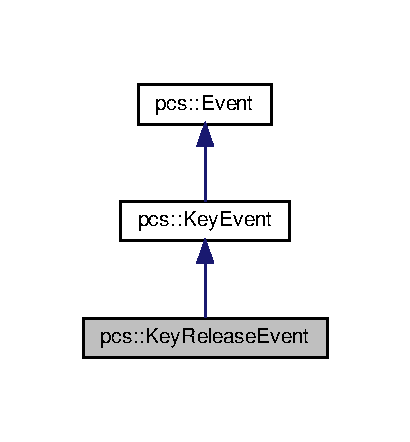
\includegraphics[width=197pt]{classpcs_1_1KeyReleaseEvent__inherit__graph}
\end{center}
\end{figure}


Collaboration diagram for pcs\+:\+:Key\+Release\+Event\+:\nopagebreak
\begin{figure}[H]
\begin{center}
\leavevmode
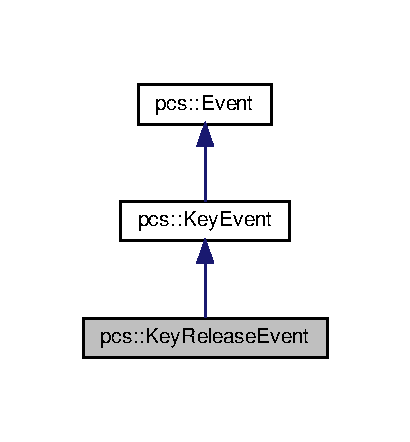
\includegraphics[width=197pt]{classpcs_1_1KeyReleaseEvent__coll__graph}
\end{center}
\end{figure}
\subsection*{Public Member Functions}
\begin{DoxyCompactItemize}
\item 
\hyperlink{classpcs_1_1KeyReleaseEvent_a03de553a1e75f029dea4f9d65760e707}{Key\+Release\+Event} (const char c)
\item 
\hyperlink{classpcs_1_1KeyReleaseEvent_aec9484a53a9b136d47cff458cd60bc91}{E\+V\+E\+N\+T\+\_\+\+T\+Y\+PE} (\hyperlink{namespacepcs_a12954f53e3d7d6a8765fd723e1ce8db4a17ee17cec34ff017c382ba1ce8dc4cdc}{Key\+Release})
\end{DoxyCompactItemize}
\subsection*{Additional Inherited Members}


\subsection{Constructor \& Destructor Documentation}
\mbox{\Hypertarget{classpcs_1_1KeyReleaseEvent_a03de553a1e75f029dea4f9d65760e707}\label{classpcs_1_1KeyReleaseEvent_a03de553a1e75f029dea4f9d65760e707}} 
\index{pcs\+::\+Key\+Release\+Event@{pcs\+::\+Key\+Release\+Event}!Key\+Release\+Event@{Key\+Release\+Event}}
\index{Key\+Release\+Event@{Key\+Release\+Event}!pcs\+::\+Key\+Release\+Event@{pcs\+::\+Key\+Release\+Event}}
\subsubsection{\texorpdfstring{Key\+Release\+Event()}{KeyReleaseEvent()}}
{\footnotesize\ttfamily pcs\+::\+Key\+Release\+Event\+::\+Key\+Release\+Event (\begin{DoxyParamCaption}\item[{const char}]{c }\end{DoxyParamCaption})\hspace{0.3cm}{\ttfamily [inline]}}



\subsection{Member Function Documentation}
\mbox{\Hypertarget{classpcs_1_1KeyReleaseEvent_aec9484a53a9b136d47cff458cd60bc91}\label{classpcs_1_1KeyReleaseEvent_aec9484a53a9b136d47cff458cd60bc91}} 
\index{pcs\+::\+Key\+Release\+Event@{pcs\+::\+Key\+Release\+Event}!E\+V\+E\+N\+T\+\_\+\+T\+Y\+PE@{E\+V\+E\+N\+T\+\_\+\+T\+Y\+PE}}
\index{E\+V\+E\+N\+T\+\_\+\+T\+Y\+PE@{E\+V\+E\+N\+T\+\_\+\+T\+Y\+PE}!pcs\+::\+Key\+Release\+Event@{pcs\+::\+Key\+Release\+Event}}
\subsubsection{\texorpdfstring{E\+V\+E\+N\+T\+\_\+\+T\+Y\+P\+E()}{EVENT\_TYPE()}}
{\footnotesize\ttfamily pcs\+::\+Key\+Release\+Event\+::\+E\+V\+E\+N\+T\+\_\+\+T\+Y\+PE (\begin{DoxyParamCaption}\item[{\hyperlink{namespacepcs_a12954f53e3d7d6a8765fd723e1ce8db4a17ee17cec34ff017c382ba1ce8dc4cdc}{Key\+Release}}]{ }\end{DoxyParamCaption})}



The documentation for this class was generated from the following file\+:\begin{DoxyCompactItemize}
\item 
include/\+Perceus/\+Core/\+Graphics/\+Rendering/\+Events/\hyperlink{KeyboardEvents_8h}{Keyboard\+Events.\+h}\end{DoxyCompactItemize}

\hypertarget{classpcs_1_1Util_1_1LinkedList}{}\section{pcs\+:\+:Util\+:\+:Linked\+List$<$ T $>$ Class Template Reference}
\label{classpcs_1_1Util_1_1LinkedList}\index{pcs\+::\+Util\+::\+Linked\+List$<$ T $>$@{pcs\+::\+Util\+::\+Linked\+List$<$ T $>$}}


{\ttfamily \#include $<$Linked\+List.\+h$>$}



Collaboration diagram for pcs\+:\+:Util\+:\+:Linked\+List$<$ T $>$\+:\nopagebreak
\begin{figure}[H]
\begin{center}
\leavevmode
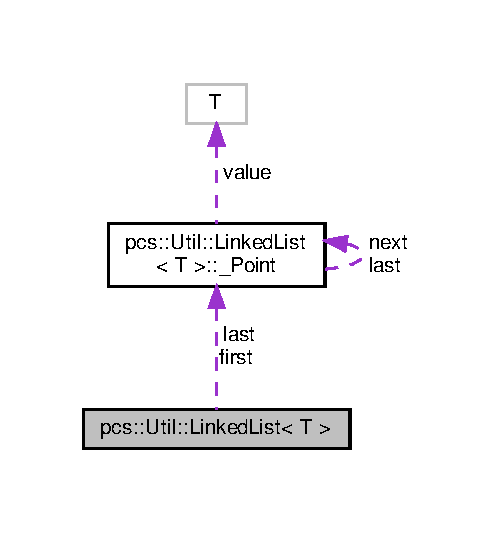
\includegraphics[width=236pt]{classpcs_1_1Util_1_1LinkedList__coll__graph}
\end{center}
\end{figure}
\subsection*{Classes}
\begin{DoxyCompactItemize}
\item 
struct \hyperlink{structpcs_1_1Util_1_1LinkedList_1_1__Point}{\+\_\+\+Point}
\end{DoxyCompactItemize}
\subsection*{Public Member Functions}
\begin{DoxyCompactItemize}
\item 
\hyperlink{classpcs_1_1Util_1_1LinkedList_ac57e454c23a32aac315f04cd2923224a}{Linked\+List} ()
\item 
void \hyperlink{classpcs_1_1Util_1_1LinkedList_a79ddaedb4fbd61886c4326a9a9c34c5d}{push} (T \&\&val)
\item 
size\+\_\+t \hyperlink{classpcs_1_1Util_1_1LinkedList_ac778698256b41a8085d3654056a4093a}{size} () const
\item 
T \& \hyperlink{classpcs_1_1Util_1_1LinkedList_a76e86131234ae5242e02a199ae2a8645}{operator\mbox{[}$\,$\mbox{]}} (size\+\_\+t index)
\end{DoxyCompactItemize}
\subsection*{Private Attributes}
\begin{DoxyCompactItemize}
\item 
size\+\_\+t \hyperlink{classpcs_1_1Util_1_1LinkedList_a3ce4faa5435a6f24917d9887ed8124d3}{\+\_\+size}
\item 
\hyperlink{structpcs_1_1Util_1_1LinkedList_1_1__Point}{\+\_\+\+Point} $\ast$ \hyperlink{classpcs_1_1Util_1_1LinkedList_a16b8eb9f35fc53d3a0d6c272aec4acc0}{first}
\item 
\hyperlink{structpcs_1_1Util_1_1LinkedList_1_1__Point}{\+\_\+\+Point} $\ast$ \hyperlink{classpcs_1_1Util_1_1LinkedList_a1760a747315ea22fe748f36c6016a32c}{last}
\end{DoxyCompactItemize}


\subsection{Constructor \& Destructor Documentation}
\mbox{\Hypertarget{classpcs_1_1Util_1_1LinkedList_ac57e454c23a32aac315f04cd2923224a}\label{classpcs_1_1Util_1_1LinkedList_ac57e454c23a32aac315f04cd2923224a}} 
\index{pcs\+::\+Util\+::\+Linked\+List@{pcs\+::\+Util\+::\+Linked\+List}!Linked\+List@{Linked\+List}}
\index{Linked\+List@{Linked\+List}!pcs\+::\+Util\+::\+Linked\+List@{pcs\+::\+Util\+::\+Linked\+List}}
\subsubsection{\texorpdfstring{Linked\+List()}{LinkedList()}}
{\footnotesize\ttfamily template$<$typename T $>$ \\
\hyperlink{classpcs_1_1Util_1_1LinkedList}{pcs\+::\+Util\+::\+Linked\+List}$<$ T $>$\+::\hyperlink{classpcs_1_1Util_1_1LinkedList}{Linked\+List} (\begin{DoxyParamCaption}{ }\end{DoxyParamCaption})\hspace{0.3cm}{\ttfamily [inline]}}



\subsection{Member Function Documentation}
\mbox{\Hypertarget{classpcs_1_1Util_1_1LinkedList_a76e86131234ae5242e02a199ae2a8645}\label{classpcs_1_1Util_1_1LinkedList_a76e86131234ae5242e02a199ae2a8645}} 
\index{pcs\+::\+Util\+::\+Linked\+List@{pcs\+::\+Util\+::\+Linked\+List}!operator\mbox{[}\mbox{]}@{operator[]}}
\index{operator\mbox{[}\mbox{]}@{operator[]}!pcs\+::\+Util\+::\+Linked\+List@{pcs\+::\+Util\+::\+Linked\+List}}
\subsubsection{\texorpdfstring{operator[]()}{operator[]()}}
{\footnotesize\ttfamily template$<$typename T $>$ \\
T \& \hyperlink{classpcs_1_1Util_1_1LinkedList}{pcs\+::\+Util\+::\+Linked\+List}$<$ T $>$\+::operator\mbox{[}$\,$\mbox{]} (\begin{DoxyParamCaption}\item[{size\+\_\+t}]{index }\end{DoxyParamCaption})}

\mbox{\Hypertarget{classpcs_1_1Util_1_1LinkedList_a79ddaedb4fbd61886c4326a9a9c34c5d}\label{classpcs_1_1Util_1_1LinkedList_a79ddaedb4fbd61886c4326a9a9c34c5d}} 
\index{pcs\+::\+Util\+::\+Linked\+List@{pcs\+::\+Util\+::\+Linked\+List}!push@{push}}
\index{push@{push}!pcs\+::\+Util\+::\+Linked\+List@{pcs\+::\+Util\+::\+Linked\+List}}
\subsubsection{\texorpdfstring{push()}{push()}}
{\footnotesize\ttfamily template$<$typename T $>$ \\
void \hyperlink{classpcs_1_1Util_1_1LinkedList}{pcs\+::\+Util\+::\+Linked\+List}$<$ T $>$\+::push (\begin{DoxyParamCaption}\item[{T \&\&}]{val }\end{DoxyParamCaption})}

\mbox{\Hypertarget{classpcs_1_1Util_1_1LinkedList_ac778698256b41a8085d3654056a4093a}\label{classpcs_1_1Util_1_1LinkedList_ac778698256b41a8085d3654056a4093a}} 
\index{pcs\+::\+Util\+::\+Linked\+List@{pcs\+::\+Util\+::\+Linked\+List}!size@{size}}
\index{size@{size}!pcs\+::\+Util\+::\+Linked\+List@{pcs\+::\+Util\+::\+Linked\+List}}
\subsubsection{\texorpdfstring{size()}{size()}}
{\footnotesize\ttfamily template$<$typename T $>$ \\
size\+\_\+t \hyperlink{classpcs_1_1Util_1_1LinkedList}{pcs\+::\+Util\+::\+Linked\+List}$<$ T $>$\+::size (\begin{DoxyParamCaption}{ }\end{DoxyParamCaption}) const}



\subsection{Member Data Documentation}
\mbox{\Hypertarget{classpcs_1_1Util_1_1LinkedList_a3ce4faa5435a6f24917d9887ed8124d3}\label{classpcs_1_1Util_1_1LinkedList_a3ce4faa5435a6f24917d9887ed8124d3}} 
\index{pcs\+::\+Util\+::\+Linked\+List@{pcs\+::\+Util\+::\+Linked\+List}!\+\_\+size@{\+\_\+size}}
\index{\+\_\+size@{\+\_\+size}!pcs\+::\+Util\+::\+Linked\+List@{pcs\+::\+Util\+::\+Linked\+List}}
\subsubsection{\texorpdfstring{\+\_\+size}{\_size}}
{\footnotesize\ttfamily template$<$typename T $>$ \\
size\+\_\+t \hyperlink{classpcs_1_1Util_1_1LinkedList}{pcs\+::\+Util\+::\+Linked\+List}$<$ T $>$\+::\+\_\+size\hspace{0.3cm}{\ttfamily [private]}}

\mbox{\Hypertarget{classpcs_1_1Util_1_1LinkedList_a16b8eb9f35fc53d3a0d6c272aec4acc0}\label{classpcs_1_1Util_1_1LinkedList_a16b8eb9f35fc53d3a0d6c272aec4acc0}} 
\index{pcs\+::\+Util\+::\+Linked\+List@{pcs\+::\+Util\+::\+Linked\+List}!first@{first}}
\index{first@{first}!pcs\+::\+Util\+::\+Linked\+List@{pcs\+::\+Util\+::\+Linked\+List}}
\subsubsection{\texorpdfstring{first}{first}}
{\footnotesize\ttfamily template$<$typename T $>$ \\
\hyperlink{structpcs_1_1Util_1_1LinkedList_1_1__Point}{\+\_\+\+Point}$\ast$ \hyperlink{classpcs_1_1Util_1_1LinkedList}{pcs\+::\+Util\+::\+Linked\+List}$<$ T $>$\+::first\hspace{0.3cm}{\ttfamily [private]}}

\mbox{\Hypertarget{classpcs_1_1Util_1_1LinkedList_a1760a747315ea22fe748f36c6016a32c}\label{classpcs_1_1Util_1_1LinkedList_a1760a747315ea22fe748f36c6016a32c}} 
\index{pcs\+::\+Util\+::\+Linked\+List@{pcs\+::\+Util\+::\+Linked\+List}!last@{last}}
\index{last@{last}!pcs\+::\+Util\+::\+Linked\+List@{pcs\+::\+Util\+::\+Linked\+List}}
\subsubsection{\texorpdfstring{last}{last}}
{\footnotesize\ttfamily template$<$typename T $>$ \\
\hyperlink{structpcs_1_1Util_1_1LinkedList_1_1__Point}{\+\_\+\+Point}$\ast$ \hyperlink{classpcs_1_1Util_1_1LinkedList}{pcs\+::\+Util\+::\+Linked\+List}$<$ T $>$\+::last\hspace{0.3cm}{\ttfamily [private]}}



The documentation for this class was generated from the following file\+:\begin{DoxyCompactItemize}
\item 
include/\+Perceus/\+Util/\+Memory/\hyperlink{LinkedList_8h}{Linked\+List.\+h}\end{DoxyCompactItemize}

\hypertarget{classpcs_1_1Log}{}\section{pcs\+:\+:Log Class Reference}
\label{classpcs_1_1Log}\index{pcs\+::\+Log@{pcs\+::\+Log}}


{\ttfamily \#include $<$Log.\+h$>$}

\subsection*{Static Public Member Functions}
\begin{DoxyCompactItemize}
\item 
static bool \hyperlink{classpcs_1_1Log_aa1d8f9f771cbe8e22171a484a00cb26a}{init} ()
\item 
static spdlog\+::logger $\ast$ \hyperlink{classpcs_1_1Log_a80c9b3bf6063be52e378daa4b12b05d9}{get\+Core} ()
\item 
static spdlog\+::logger $\ast$ \hyperlink{classpcs_1_1Log_aaa4d7462a9140c5c71cf55320a233cbc}{get\+Client} ()
\end{DoxyCompactItemize}
\subsection*{Static Private Attributes}
\begin{DoxyCompactItemize}
\item 
static spdlog\+::logger $\ast$ \hyperlink{classpcs_1_1Log_a10c192099a05bf06b0b45ff11d6df3fc}{core\+Logger} = nullptr
\item 
static spdlog\+::logger $\ast$ \hyperlink{classpcs_1_1Log_aaaf4f92cf3f544bec35e425c2e3dbf90}{client\+Logger} = nullptr
\end{DoxyCompactItemize}


\subsection{Member Function Documentation}
\mbox{\Hypertarget{classpcs_1_1Log_aaa4d7462a9140c5c71cf55320a233cbc}\label{classpcs_1_1Log_aaa4d7462a9140c5c71cf55320a233cbc}} 
\index{pcs\+::\+Log@{pcs\+::\+Log}!get\+Client@{get\+Client}}
\index{get\+Client@{get\+Client}!pcs\+::\+Log@{pcs\+::\+Log}}
\subsubsection{\texorpdfstring{get\+Client()}{getClient()}}
{\footnotesize\ttfamily static spdlog\+::logger$\ast$ pcs\+::\+Log\+::get\+Client (\begin{DoxyParamCaption}{ }\end{DoxyParamCaption})\hspace{0.3cm}{\ttfamily [inline]}, {\ttfamily [static]}}

\mbox{\Hypertarget{classpcs_1_1Log_a80c9b3bf6063be52e378daa4b12b05d9}\label{classpcs_1_1Log_a80c9b3bf6063be52e378daa4b12b05d9}} 
\index{pcs\+::\+Log@{pcs\+::\+Log}!get\+Core@{get\+Core}}
\index{get\+Core@{get\+Core}!pcs\+::\+Log@{pcs\+::\+Log}}
\subsubsection{\texorpdfstring{get\+Core()}{getCore()}}
{\footnotesize\ttfamily static spdlog\+::logger$\ast$ pcs\+::\+Log\+::get\+Core (\begin{DoxyParamCaption}{ }\end{DoxyParamCaption})\hspace{0.3cm}{\ttfamily [inline]}, {\ttfamily [static]}}

\mbox{\Hypertarget{classpcs_1_1Log_aa1d8f9f771cbe8e22171a484a00cb26a}\label{classpcs_1_1Log_aa1d8f9f771cbe8e22171a484a00cb26a}} 
\index{pcs\+::\+Log@{pcs\+::\+Log}!init@{init}}
\index{init@{init}!pcs\+::\+Log@{pcs\+::\+Log}}
\subsubsection{\texorpdfstring{init()}{init()}}
{\footnotesize\ttfamily bool pcs\+::\+Log\+::init (\begin{DoxyParamCaption}{ }\end{DoxyParamCaption})\hspace{0.3cm}{\ttfamily [static]}}



\subsection{Member Data Documentation}
\mbox{\Hypertarget{classpcs_1_1Log_aaaf4f92cf3f544bec35e425c2e3dbf90}\label{classpcs_1_1Log_aaaf4f92cf3f544bec35e425c2e3dbf90}} 
\index{pcs\+::\+Log@{pcs\+::\+Log}!client\+Logger@{client\+Logger}}
\index{client\+Logger@{client\+Logger}!pcs\+::\+Log@{pcs\+::\+Log}}
\subsubsection{\texorpdfstring{client\+Logger}{clientLogger}}
{\footnotesize\ttfamily spdlog\+::logger $\ast$ pcs\+::\+Log\+::client\+Logger = nullptr\hspace{0.3cm}{\ttfamily [static]}, {\ttfamily [private]}}

\mbox{\Hypertarget{classpcs_1_1Log_a10c192099a05bf06b0b45ff11d6df3fc}\label{classpcs_1_1Log_a10c192099a05bf06b0b45ff11d6df3fc}} 
\index{pcs\+::\+Log@{pcs\+::\+Log}!core\+Logger@{core\+Logger}}
\index{core\+Logger@{core\+Logger}!pcs\+::\+Log@{pcs\+::\+Log}}
\subsubsection{\texorpdfstring{core\+Logger}{coreLogger}}
{\footnotesize\ttfamily spdlog\+::logger $\ast$ pcs\+::\+Log\+::core\+Logger = nullptr\hspace{0.3cm}{\ttfamily [static]}, {\ttfamily [private]}}



The documentation for this class was generated from the following files\+:\begin{DoxyCompactItemize}
\item 
include/\+Perceus/\+Util/\hyperlink{Log_8h}{Log.\+h}\item 
src/\+Util/\hyperlink{Log_8cpp}{Log.\+cpp}\end{DoxyCompactItemize}

\hypertarget{structpcs_1_1Mat4f}{}\section{pcs\+:\+:Mat4f Struct Reference}
\label{structpcs_1_1Mat4f}\index{pcs\+::\+Mat4f@{pcs\+::\+Mat4f}}


{\ttfamily \#include $<$Matrix.\+h$>$}

\subsection*{Public Member Functions}
\begin{DoxyCompactItemize}
\item 
void \hyperlink{structpcs_1_1Mat4f_af43fedb87b0bf46325895dd098ae4600}{to\+Identity} ()
\item 
\hyperlink{namespacepcs_a826b4146f438aa3a4c6a5c157bc8dea2}{Vec4f} \hyperlink{structpcs_1_1Mat4f_a0703785e2c39f97f89c8305578f40ed8}{get\+Row} (int index)
\item 
\hyperlink{structpcs_1_1Mat4f}{Mat4f} \hyperlink{structpcs_1_1Mat4f_abf5cbb6f96fe61bbd09820868fe23cae}{operator$\ast$} (const \hyperlink{structpcs_1_1Mat4f}{Mat4f} \&mat) const
\end{DoxyCompactItemize}
\subsection*{Static Public Member Functions}
\begin{DoxyCompactItemize}
\item 
static \hyperlink{structpcs_1_1Mat4f}{Mat4f} \hyperlink{structpcs_1_1Mat4f_a3c7026479b0855ee1e1a4ff962872a95}{make\+Identity} ()
\item 
static \hyperlink{structpcs_1_1Mat4f}{Mat4f} \hyperlink{structpcs_1_1Mat4f_af221a379a3419f70b69c0339d499434c}{make\+Translation} (const float x, const float y, const float z)
\item 
static \hyperlink{structpcs_1_1Mat4f}{Mat4f} \hyperlink{structpcs_1_1Mat4f_aab015352eaa466dbb0c5c11d361f85af}{make\+Translation} (const \hyperlink{namespacepcs_a68e0f517680976c17c810ffe6952cbab}{Vec3f} \&vec)
\item 
static \hyperlink{structpcs_1_1Mat4f}{Mat4f} \hyperlink{structpcs_1_1Mat4f_a0bacf80f2ce6f50ad379299010a7cc44}{make\+Rotation} (const float x, const float y, const float z)
\item 
static \hyperlink{structpcs_1_1Mat4f}{Mat4f} \hyperlink{structpcs_1_1Mat4f_a46b7418d93345a9609304b54fea5ed98}{make\+Rotation} (const \hyperlink{namespacepcs_a68e0f517680976c17c810ffe6952cbab}{Vec3f} \&rot)
\item 
static \hyperlink{structpcs_1_1Mat4f}{Mat4f} \hyperlink{structpcs_1_1Mat4f_a76bf290cb265ba821bb1bb04b822f361}{make\+Scale} (const float x, const float y, const float z)
\item 
static \hyperlink{structpcs_1_1Mat4f}{Mat4f} \hyperlink{structpcs_1_1Mat4f_a7d4f035fc516774ddc99f17333712a69}{make\+Scale} (const \hyperlink{namespacepcs_a68e0f517680976c17c810ffe6952cbab}{Vec3f} \&rot)
\end{DoxyCompactItemize}
\subsection*{Public Attributes}
\begin{DoxyCompactItemize}
\item 
float \hyperlink{structpcs_1_1Mat4f_ad5835795f842580da5e36a70c39cc6c9}{m} \mbox{[}4\mbox{]}\mbox{[}4\mbox{]}
\end{DoxyCompactItemize}


\subsection{Member Function Documentation}
\mbox{\Hypertarget{structpcs_1_1Mat4f_a0703785e2c39f97f89c8305578f40ed8}\label{structpcs_1_1Mat4f_a0703785e2c39f97f89c8305578f40ed8}} 
\index{pcs\+::\+Mat4f@{pcs\+::\+Mat4f}!get\+Row@{get\+Row}}
\index{get\+Row@{get\+Row}!pcs\+::\+Mat4f@{pcs\+::\+Mat4f}}
\subsubsection{\texorpdfstring{get\+Row()}{getRow()}}
{\footnotesize\ttfamily \hyperlink{namespacepcs_a826b4146f438aa3a4c6a5c157bc8dea2}{Vec4f} pcs\+::\+Mat4f\+::get\+Row (\begin{DoxyParamCaption}\item[{int}]{index }\end{DoxyParamCaption})\hspace{0.3cm}{\ttfamily [inline]}}

\mbox{\Hypertarget{structpcs_1_1Mat4f_a3c7026479b0855ee1e1a4ff962872a95}\label{structpcs_1_1Mat4f_a3c7026479b0855ee1e1a4ff962872a95}} 
\index{pcs\+::\+Mat4f@{pcs\+::\+Mat4f}!make\+Identity@{make\+Identity}}
\index{make\+Identity@{make\+Identity}!pcs\+::\+Mat4f@{pcs\+::\+Mat4f}}
\subsubsection{\texorpdfstring{make\+Identity()}{makeIdentity()}}
{\footnotesize\ttfamily static \hyperlink{structpcs_1_1Mat4f}{Mat4f} pcs\+::\+Mat4f\+::make\+Identity (\begin{DoxyParamCaption}{ }\end{DoxyParamCaption})\hspace{0.3cm}{\ttfamily [inline]}, {\ttfamily [static]}}

\mbox{\Hypertarget{structpcs_1_1Mat4f_a0bacf80f2ce6f50ad379299010a7cc44}\label{structpcs_1_1Mat4f_a0bacf80f2ce6f50ad379299010a7cc44}} 
\index{pcs\+::\+Mat4f@{pcs\+::\+Mat4f}!make\+Rotation@{make\+Rotation}}
\index{make\+Rotation@{make\+Rotation}!pcs\+::\+Mat4f@{pcs\+::\+Mat4f}}
\subsubsection{\texorpdfstring{make\+Rotation()}{makeRotation()}\hspace{0.1cm}{\footnotesize\ttfamily [1/2]}}
{\footnotesize\ttfamily static \hyperlink{structpcs_1_1Mat4f}{Mat4f} pcs\+::\+Mat4f\+::make\+Rotation (\begin{DoxyParamCaption}\item[{const float}]{x,  }\item[{const float}]{y,  }\item[{const float}]{z }\end{DoxyParamCaption})\hspace{0.3cm}{\ttfamily [inline]}, {\ttfamily [static]}}

\mbox{\Hypertarget{structpcs_1_1Mat4f_a46b7418d93345a9609304b54fea5ed98}\label{structpcs_1_1Mat4f_a46b7418d93345a9609304b54fea5ed98}} 
\index{pcs\+::\+Mat4f@{pcs\+::\+Mat4f}!make\+Rotation@{make\+Rotation}}
\index{make\+Rotation@{make\+Rotation}!pcs\+::\+Mat4f@{pcs\+::\+Mat4f}}
\subsubsection{\texorpdfstring{make\+Rotation()}{makeRotation()}\hspace{0.1cm}{\footnotesize\ttfamily [2/2]}}
{\footnotesize\ttfamily static \hyperlink{structpcs_1_1Mat4f}{Mat4f} pcs\+::\+Mat4f\+::make\+Rotation (\begin{DoxyParamCaption}\item[{const \hyperlink{namespacepcs_a68e0f517680976c17c810ffe6952cbab}{Vec3f} \&}]{rot }\end{DoxyParamCaption})\hspace{0.3cm}{\ttfamily [inline]}, {\ttfamily [static]}}

\mbox{\Hypertarget{structpcs_1_1Mat4f_a76bf290cb265ba821bb1bb04b822f361}\label{structpcs_1_1Mat4f_a76bf290cb265ba821bb1bb04b822f361}} 
\index{pcs\+::\+Mat4f@{pcs\+::\+Mat4f}!make\+Scale@{make\+Scale}}
\index{make\+Scale@{make\+Scale}!pcs\+::\+Mat4f@{pcs\+::\+Mat4f}}
\subsubsection{\texorpdfstring{make\+Scale()}{makeScale()}\hspace{0.1cm}{\footnotesize\ttfamily [1/2]}}
{\footnotesize\ttfamily static \hyperlink{structpcs_1_1Mat4f}{Mat4f} pcs\+::\+Mat4f\+::make\+Scale (\begin{DoxyParamCaption}\item[{const float}]{x,  }\item[{const float}]{y,  }\item[{const float}]{z }\end{DoxyParamCaption})\hspace{0.3cm}{\ttfamily [inline]}, {\ttfamily [static]}}

\mbox{\Hypertarget{structpcs_1_1Mat4f_a7d4f035fc516774ddc99f17333712a69}\label{structpcs_1_1Mat4f_a7d4f035fc516774ddc99f17333712a69}} 
\index{pcs\+::\+Mat4f@{pcs\+::\+Mat4f}!make\+Scale@{make\+Scale}}
\index{make\+Scale@{make\+Scale}!pcs\+::\+Mat4f@{pcs\+::\+Mat4f}}
\subsubsection{\texorpdfstring{make\+Scale()}{makeScale()}\hspace{0.1cm}{\footnotesize\ttfamily [2/2]}}
{\footnotesize\ttfamily static \hyperlink{structpcs_1_1Mat4f}{Mat4f} pcs\+::\+Mat4f\+::make\+Scale (\begin{DoxyParamCaption}\item[{const \hyperlink{namespacepcs_a68e0f517680976c17c810ffe6952cbab}{Vec3f} \&}]{rot }\end{DoxyParamCaption})\hspace{0.3cm}{\ttfamily [inline]}, {\ttfamily [static]}}

\mbox{\Hypertarget{structpcs_1_1Mat4f_af221a379a3419f70b69c0339d499434c}\label{structpcs_1_1Mat4f_af221a379a3419f70b69c0339d499434c}} 
\index{pcs\+::\+Mat4f@{pcs\+::\+Mat4f}!make\+Translation@{make\+Translation}}
\index{make\+Translation@{make\+Translation}!pcs\+::\+Mat4f@{pcs\+::\+Mat4f}}
\subsubsection{\texorpdfstring{make\+Translation()}{makeTranslation()}\hspace{0.1cm}{\footnotesize\ttfamily [1/2]}}
{\footnotesize\ttfamily static \hyperlink{structpcs_1_1Mat4f}{Mat4f} pcs\+::\+Mat4f\+::make\+Translation (\begin{DoxyParamCaption}\item[{const float}]{x,  }\item[{const float}]{y,  }\item[{const float}]{z }\end{DoxyParamCaption})\hspace{0.3cm}{\ttfamily [inline]}, {\ttfamily [static]}}

\mbox{\Hypertarget{structpcs_1_1Mat4f_aab015352eaa466dbb0c5c11d361f85af}\label{structpcs_1_1Mat4f_aab015352eaa466dbb0c5c11d361f85af}} 
\index{pcs\+::\+Mat4f@{pcs\+::\+Mat4f}!make\+Translation@{make\+Translation}}
\index{make\+Translation@{make\+Translation}!pcs\+::\+Mat4f@{pcs\+::\+Mat4f}}
\subsubsection{\texorpdfstring{make\+Translation()}{makeTranslation()}\hspace{0.1cm}{\footnotesize\ttfamily [2/2]}}
{\footnotesize\ttfamily static \hyperlink{structpcs_1_1Mat4f}{Mat4f} pcs\+::\+Mat4f\+::make\+Translation (\begin{DoxyParamCaption}\item[{const \hyperlink{namespacepcs_a68e0f517680976c17c810ffe6952cbab}{Vec3f} \&}]{vec }\end{DoxyParamCaption})\hspace{0.3cm}{\ttfamily [inline]}, {\ttfamily [static]}}

\mbox{\Hypertarget{structpcs_1_1Mat4f_abf5cbb6f96fe61bbd09820868fe23cae}\label{structpcs_1_1Mat4f_abf5cbb6f96fe61bbd09820868fe23cae}} 
\index{pcs\+::\+Mat4f@{pcs\+::\+Mat4f}!operator$\ast$@{operator$\ast$}}
\index{operator$\ast$@{operator$\ast$}!pcs\+::\+Mat4f@{pcs\+::\+Mat4f}}
\subsubsection{\texorpdfstring{operator$\ast$()}{operator*()}}
{\footnotesize\ttfamily \hyperlink{structpcs_1_1Mat4f}{Mat4f} pcs\+::\+Mat4f\+::operator$\ast$ (\begin{DoxyParamCaption}\item[{const \hyperlink{structpcs_1_1Mat4f}{Mat4f} \&}]{mat }\end{DoxyParamCaption}) const\hspace{0.3cm}{\ttfamily [inline]}}

\mbox{\Hypertarget{structpcs_1_1Mat4f_af43fedb87b0bf46325895dd098ae4600}\label{structpcs_1_1Mat4f_af43fedb87b0bf46325895dd098ae4600}} 
\index{pcs\+::\+Mat4f@{pcs\+::\+Mat4f}!to\+Identity@{to\+Identity}}
\index{to\+Identity@{to\+Identity}!pcs\+::\+Mat4f@{pcs\+::\+Mat4f}}
\subsubsection{\texorpdfstring{to\+Identity()}{toIdentity()}}
{\footnotesize\ttfamily void pcs\+::\+Mat4f\+::to\+Identity (\begin{DoxyParamCaption}{ }\end{DoxyParamCaption})\hspace{0.3cm}{\ttfamily [inline]}}



\subsection{Member Data Documentation}
\mbox{\Hypertarget{structpcs_1_1Mat4f_ad5835795f842580da5e36a70c39cc6c9}\label{structpcs_1_1Mat4f_ad5835795f842580da5e36a70c39cc6c9}} 
\index{pcs\+::\+Mat4f@{pcs\+::\+Mat4f}!m@{m}}
\index{m@{m}!pcs\+::\+Mat4f@{pcs\+::\+Mat4f}}
\subsubsection{\texorpdfstring{m}{m}}
{\footnotesize\ttfamily float pcs\+::\+Mat4f\+::m\mbox{[}4\mbox{]}\mbox{[}4\mbox{]}}



The documentation for this struct was generated from the following file\+:\begin{DoxyCompactItemize}
\item 
include/\+Perceus/\+Data/\hyperlink{Matrix_8h}{Matrix.\+h}\end{DoxyCompactItemize}

\hypertarget{classpcs_1_1Model}{}\section{pcs\+:\+:Model Class Reference}
\label{classpcs_1_1Model}\index{pcs\+::\+Model@{pcs\+::\+Model}}


{\ttfamily \#include $<$Model.\+h$>$}



Inheritance diagram for pcs\+:\+:Model\+:\nopagebreak
\begin{figure}[H]
\begin{center}
\leavevmode
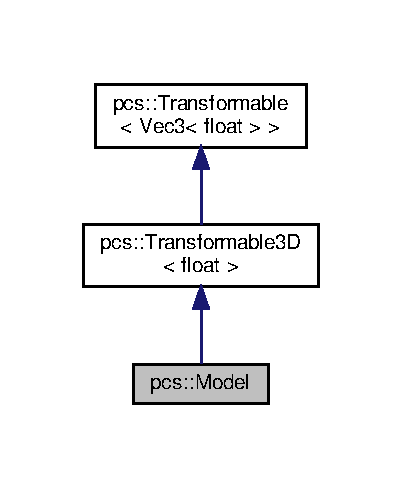
\includegraphics[width=193pt]{classpcs_1_1Model__inherit__graph}
\end{center}
\end{figure}


Collaboration diagram for pcs\+:\+:Model\+:\nopagebreak
\begin{figure}[H]
\begin{center}
\leavevmode
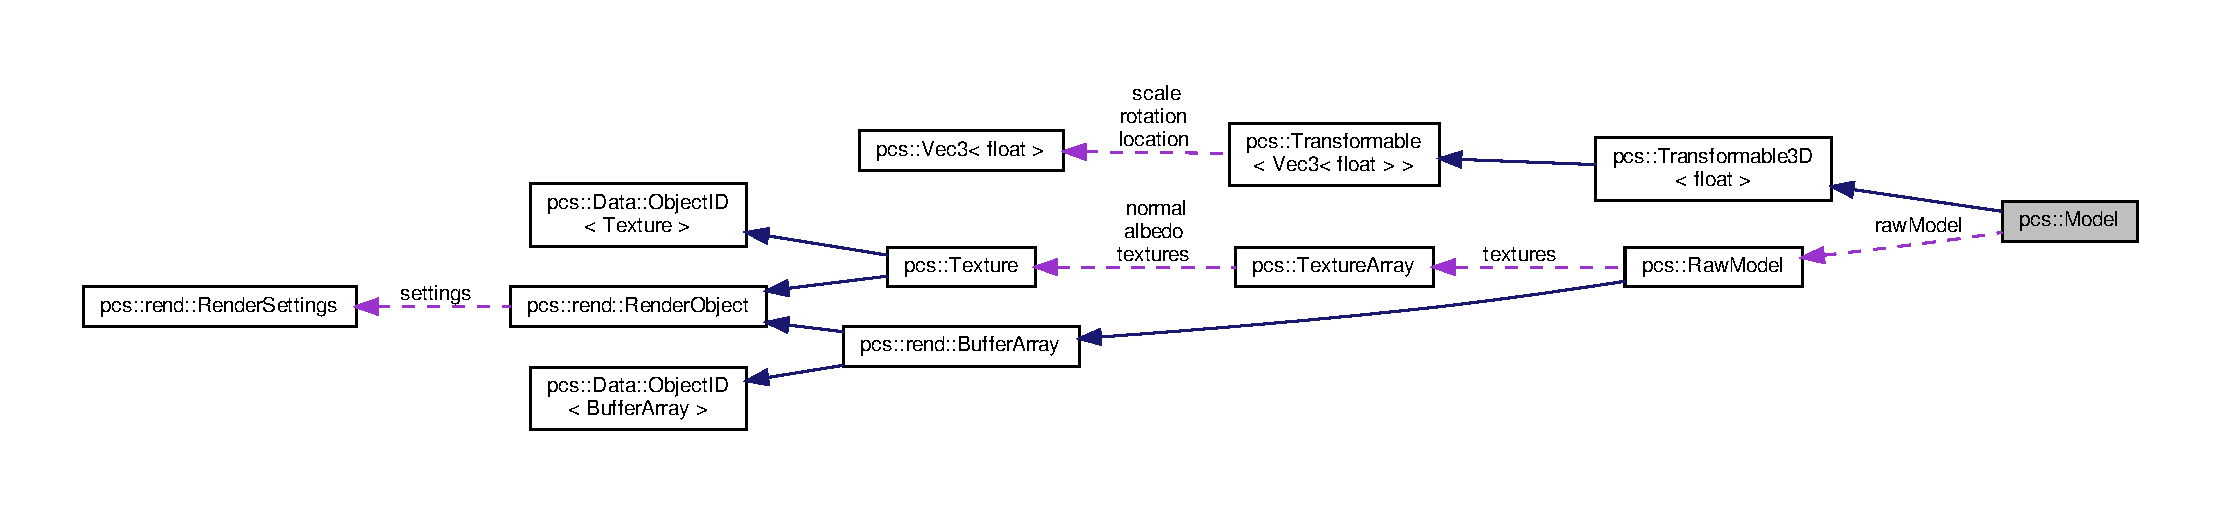
\includegraphics[width=350pt]{classpcs_1_1Model__coll__graph}
\end{center}
\end{figure}
\subsection*{Public Member Functions}
\begin{DoxyCompactItemize}
\item 
\hyperlink{classpcs_1_1Model_a353c041e246baa1bc4ab54b23918dfb9}{Model} (\hyperlink{classpcs_1_1RawModel}{Raw\+Model} $\ast$rm)
\item 
virtual void \hyperlink{classpcs_1_1Model_a143831f415158255b910e25ac542de19}{update} (double delta\+Time)
\item 
\hyperlink{structpcs_1_1Mat4f}{Mat4f} \hyperlink{classpcs_1_1Model_a70cb396d1e636d013ec22257be078120}{get\+Model\+Matrix} ()
\item 
\hyperlink{classpcs_1_1RawModel}{Raw\+Model} $\ast$ \hyperlink{classpcs_1_1Model_aaffd9c9e96661db20405c0c12138c940}{get\+Raw\+Model} ()
\end{DoxyCompactItemize}
\subsection*{Private Attributes}
\begin{DoxyCompactItemize}
\item 
\hyperlink{classpcs_1_1RawModel}{Raw\+Model} $\ast$ \hyperlink{classpcs_1_1Model_a40bca7561aa0a79a5d0d386d1b875bfe}{raw\+Model}
\end{DoxyCompactItemize}


\subsection{Constructor \& Destructor Documentation}
\mbox{\Hypertarget{classpcs_1_1Model_a353c041e246baa1bc4ab54b23918dfb9}\label{classpcs_1_1Model_a353c041e246baa1bc4ab54b23918dfb9}} 
\index{pcs\+::\+Model@{pcs\+::\+Model}!Model@{Model}}
\index{Model@{Model}!pcs\+::\+Model@{pcs\+::\+Model}}
\subsubsection{\texorpdfstring{Model()}{Model()}}
{\footnotesize\ttfamily pcs\+::\+Model\+::\+Model (\begin{DoxyParamCaption}\item[{\hyperlink{classpcs_1_1RawModel}{Raw\+Model} $\ast$}]{rm }\end{DoxyParamCaption})}



\subsection{Member Function Documentation}
\mbox{\Hypertarget{classpcs_1_1Model_a70cb396d1e636d013ec22257be078120}\label{classpcs_1_1Model_a70cb396d1e636d013ec22257be078120}} 
\index{pcs\+::\+Model@{pcs\+::\+Model}!get\+Model\+Matrix@{get\+Model\+Matrix}}
\index{get\+Model\+Matrix@{get\+Model\+Matrix}!pcs\+::\+Model@{pcs\+::\+Model}}
\subsubsection{\texorpdfstring{get\+Model\+Matrix()}{getModelMatrix()}}
{\footnotesize\ttfamily \hyperlink{structpcs_1_1Mat4f}{Mat4f} pcs\+::\+Model\+::get\+Model\+Matrix (\begin{DoxyParamCaption}{ }\end{DoxyParamCaption})}

\mbox{\Hypertarget{classpcs_1_1Model_aaffd9c9e96661db20405c0c12138c940}\label{classpcs_1_1Model_aaffd9c9e96661db20405c0c12138c940}} 
\index{pcs\+::\+Model@{pcs\+::\+Model}!get\+Raw\+Model@{get\+Raw\+Model}}
\index{get\+Raw\+Model@{get\+Raw\+Model}!pcs\+::\+Model@{pcs\+::\+Model}}
\subsubsection{\texorpdfstring{get\+Raw\+Model()}{getRawModel()}}
{\footnotesize\ttfamily \hyperlink{classpcs_1_1RawModel}{Raw\+Model}$\ast$ pcs\+::\+Model\+::get\+Raw\+Model (\begin{DoxyParamCaption}{ }\end{DoxyParamCaption})\hspace{0.3cm}{\ttfamily [inline]}}

\mbox{\Hypertarget{classpcs_1_1Model_a143831f415158255b910e25ac542de19}\label{classpcs_1_1Model_a143831f415158255b910e25ac542de19}} 
\index{pcs\+::\+Model@{pcs\+::\+Model}!update@{update}}
\index{update@{update}!pcs\+::\+Model@{pcs\+::\+Model}}
\subsubsection{\texorpdfstring{update()}{update()}}
{\footnotesize\ttfamily virtual void pcs\+::\+Model\+::update (\begin{DoxyParamCaption}\item[{double}]{delta\+Time }\end{DoxyParamCaption})\hspace{0.3cm}{\ttfamily [inline]}, {\ttfamily [virtual]}}



\subsection{Member Data Documentation}
\mbox{\Hypertarget{classpcs_1_1Model_a40bca7561aa0a79a5d0d386d1b875bfe}\label{classpcs_1_1Model_a40bca7561aa0a79a5d0d386d1b875bfe}} 
\index{pcs\+::\+Model@{pcs\+::\+Model}!raw\+Model@{raw\+Model}}
\index{raw\+Model@{raw\+Model}!pcs\+::\+Model@{pcs\+::\+Model}}
\subsubsection{\texorpdfstring{raw\+Model}{rawModel}}
{\footnotesize\ttfamily \hyperlink{classpcs_1_1RawModel}{Raw\+Model}$\ast$ pcs\+::\+Model\+::raw\+Model\hspace{0.3cm}{\ttfamily [private]}}



The documentation for this class was generated from the following files\+:\begin{DoxyCompactItemize}
\item 
include/\+Perceus/\+Core/\+Graphics/\+Entities/\hyperlink{Model_8h}{Model.\+h}\item 
src/\+Core/\+Graphics/\+Entities/\hyperlink{Model_8cpp}{Model.\+cpp}\end{DoxyCompactItemize}

\hypertarget{structpcs_1_1Data_1_1NonCopyable}{}\section{pcs\+:\+:Data\+:\+:Non\+Copyable Struct Reference}
\label{structpcs_1_1Data_1_1NonCopyable}\index{pcs\+::\+Data\+::\+Non\+Copyable@{pcs\+::\+Data\+::\+Non\+Copyable}}


{\ttfamily \#include $<$Non\+Copyable.\+h$>$}



Inheritance diagram for pcs\+:\+:Data\+:\+:Non\+Copyable\+:\nopagebreak
\begin{figure}[H]
\begin{center}
\leavevmode
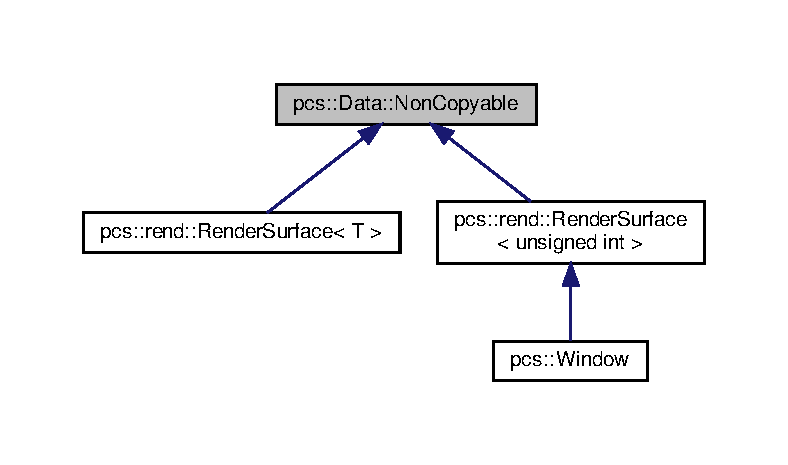
\includegraphics[width=350pt]{structpcs_1_1Data_1_1NonCopyable__inherit__graph}
\end{center}
\end{figure}
\subsection*{Public Member Functions}
\begin{DoxyCompactItemize}
\item 
\hyperlink{structpcs_1_1Data_1_1NonCopyable_ac9cde01db2d5ba115c033ae5ce13a11f}{Non\+Copyable} (const \hyperlink{structpcs_1_1Data_1_1NonCopyable}{Non\+Copyable} \&)
\item 
\hyperlink{structpcs_1_1Data_1_1NonCopyable}{Non\+Copyable} \& \hyperlink{structpcs_1_1Data_1_1NonCopyable_a3fec6abd7a92cc27e19fe7361b3f0c24}{operator=} (const \hyperlink{structpcs_1_1Data_1_1NonCopyable}{Non\+Copyable} \&)
\end{DoxyCompactItemize}
\subsection*{Protected Member Functions}
\begin{DoxyCompactItemize}
\item 
\hyperlink{structpcs_1_1Data_1_1NonCopyable_aad220ecfe40ad6fa4f57450db4589750}{Non\+Copyable} ()
\item 
\hyperlink{structpcs_1_1Data_1_1NonCopyable_aaaf234adb2a742fee93e4eee336c1dcc}{$\sim$\+Non\+Copyable} ()
\end{DoxyCompactItemize}


\subsection{Constructor \& Destructor Documentation}
\mbox{\Hypertarget{structpcs_1_1Data_1_1NonCopyable_aad220ecfe40ad6fa4f57450db4589750}\label{structpcs_1_1Data_1_1NonCopyable_aad220ecfe40ad6fa4f57450db4589750}} 
\index{pcs\+::\+Data\+::\+Non\+Copyable@{pcs\+::\+Data\+::\+Non\+Copyable}!Non\+Copyable@{Non\+Copyable}}
\index{Non\+Copyable@{Non\+Copyable}!pcs\+::\+Data\+::\+Non\+Copyable@{pcs\+::\+Data\+::\+Non\+Copyable}}
\subsubsection{\texorpdfstring{Non\+Copyable()}{NonCopyable()}\hspace{0.1cm}{\footnotesize\ttfamily [1/2]}}
{\footnotesize\ttfamily pcs\+::\+Data\+::\+Non\+Copyable\+::\+Non\+Copyable (\begin{DoxyParamCaption}{ }\end{DoxyParamCaption})\hspace{0.3cm}{\ttfamily [inline]}, {\ttfamily [protected]}}

\mbox{\Hypertarget{structpcs_1_1Data_1_1NonCopyable_aaaf234adb2a742fee93e4eee336c1dcc}\label{structpcs_1_1Data_1_1NonCopyable_aaaf234adb2a742fee93e4eee336c1dcc}} 
\index{pcs\+::\+Data\+::\+Non\+Copyable@{pcs\+::\+Data\+::\+Non\+Copyable}!````~Non\+Copyable@{$\sim$\+Non\+Copyable}}
\index{````~Non\+Copyable@{$\sim$\+Non\+Copyable}!pcs\+::\+Data\+::\+Non\+Copyable@{pcs\+::\+Data\+::\+Non\+Copyable}}
\subsubsection{\texorpdfstring{$\sim$\+Non\+Copyable()}{~NonCopyable()}}
{\footnotesize\ttfamily pcs\+::\+Data\+::\+Non\+Copyable\+::$\sim$\+Non\+Copyable (\begin{DoxyParamCaption}{ }\end{DoxyParamCaption})\hspace{0.3cm}{\ttfamily [inline]}, {\ttfamily [protected]}}

\mbox{\Hypertarget{structpcs_1_1Data_1_1NonCopyable_ac9cde01db2d5ba115c033ae5ce13a11f}\label{structpcs_1_1Data_1_1NonCopyable_ac9cde01db2d5ba115c033ae5ce13a11f}} 
\index{pcs\+::\+Data\+::\+Non\+Copyable@{pcs\+::\+Data\+::\+Non\+Copyable}!Non\+Copyable@{Non\+Copyable}}
\index{Non\+Copyable@{Non\+Copyable}!pcs\+::\+Data\+::\+Non\+Copyable@{pcs\+::\+Data\+::\+Non\+Copyable}}
\subsubsection{\texorpdfstring{Non\+Copyable()}{NonCopyable()}\hspace{0.1cm}{\footnotesize\ttfamily [2/2]}}
{\footnotesize\ttfamily pcs\+::\+Data\+::\+Non\+Copyable\+::\+Non\+Copyable (\begin{DoxyParamCaption}\item[{const \hyperlink{structpcs_1_1Data_1_1NonCopyable}{Non\+Copyable} \&}]{ }\end{DoxyParamCaption})}



\subsection{Member Function Documentation}
\mbox{\Hypertarget{structpcs_1_1Data_1_1NonCopyable_a3fec6abd7a92cc27e19fe7361b3f0c24}\label{structpcs_1_1Data_1_1NonCopyable_a3fec6abd7a92cc27e19fe7361b3f0c24}} 
\index{pcs\+::\+Data\+::\+Non\+Copyable@{pcs\+::\+Data\+::\+Non\+Copyable}!operator=@{operator=}}
\index{operator=@{operator=}!pcs\+::\+Data\+::\+Non\+Copyable@{pcs\+::\+Data\+::\+Non\+Copyable}}
\subsubsection{\texorpdfstring{operator=()}{operator=()}}
{\footnotesize\ttfamily \hyperlink{structpcs_1_1Data_1_1NonCopyable}{Non\+Copyable}\& pcs\+::\+Data\+::\+Non\+Copyable\+::operator= (\begin{DoxyParamCaption}\item[{const \hyperlink{structpcs_1_1Data_1_1NonCopyable}{Non\+Copyable} \&}]{ }\end{DoxyParamCaption})}



The documentation for this struct was generated from the following file\+:\begin{DoxyCompactItemize}
\item 
include/\+Perceus/\+Data/\hyperlink{NonCopyable_8h}{Non\+Copyable.\+h}\end{DoxyCompactItemize}

\hypertarget{classpcs_1_1Data_1_1ObjectID}{}\section{pcs\+:\+:Data\+:\+:Object\+ID$<$ T, R $>$ Class Template Reference}
\label{classpcs_1_1Data_1_1ObjectID}\index{pcs\+::\+Data\+::\+Object\+I\+D$<$ T, R $>$@{pcs\+::\+Data\+::\+Object\+I\+D$<$ T, R $>$}}


Class that handles an object\textquotesingle{}s unique ID.  




{\ttfamily \#include $<$Object\+I\+D.\+h$>$}



Collaboration diagram for pcs\+:\+:Data\+:\+:Object\+ID$<$ T, R $>$\+:\nopagebreak
\begin{figure}[H]
\begin{center}
\leavevmode
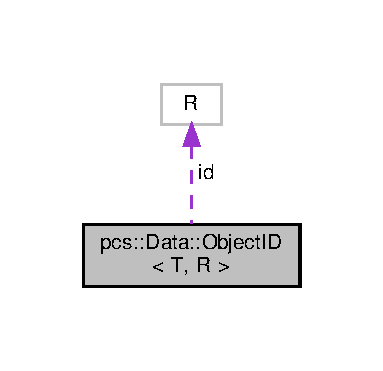
\includegraphics[width=184pt]{classpcs_1_1Data_1_1ObjectID__coll__graph}
\end{center}
\end{figure}
\subsection*{Public Member Functions}
\begin{DoxyCompactItemize}
\item 
\hyperlink{classpcs_1_1Data_1_1ObjectID_aa94cbbd6c36354f876de0b6847a07ed0}{Object\+ID} ()
\begin{DoxyCompactList}\small\item\em Constructs a new \hyperlink{classpcs_1_1Data_1_1ObjectID}{Object\+ID}. \end{DoxyCompactList}\item 
R \& \hyperlink{classpcs_1_1Data_1_1ObjectID_aaee6ebc98b85f079ff8597f5c6f39cb3}{get\+ID} ()
\begin{DoxyCompactList}\small\item\em Gets the ID. \end{DoxyCompactList}\end{DoxyCompactItemize}
\subsection*{Protected Member Functions}
\begin{DoxyCompactItemize}
\item 
virtual R \hyperlink{classpcs_1_1Data_1_1ObjectID_a01456dc5ee820984c83c089e413255ec}{get\+Next} ()
\begin{DoxyCompactList}\small\item\em Get the next ID. \end{DoxyCompactList}\end{DoxyCompactItemize}
\subsection*{Protected Attributes}
\begin{DoxyCompactItemize}
\item 
R \hyperlink{classpcs_1_1Data_1_1ObjectID_a69a11bfb96a9078095de9bb139b06913}{id}
\begin{DoxyCompactList}\small\item\em Current ID. \end{DoxyCompactList}\end{DoxyCompactItemize}


\subsection{Detailed Description}
\subsubsection*{template$<$typename T, typename R = unsigned int$>$\newline
class pcs\+::\+Data\+::\+Object\+I\+D$<$ T, R $>$}

Class that handles an object\textquotesingle{}s unique ID. 


\begin{DoxyTemplParams}{Template Parameters}
{\em T} & Class of which the object is declared \\
\hline
\end{DoxyTemplParams}


\subsection{Constructor \& Destructor Documentation}
\mbox{\Hypertarget{classpcs_1_1Data_1_1ObjectID_aa94cbbd6c36354f876de0b6847a07ed0}\label{classpcs_1_1Data_1_1ObjectID_aa94cbbd6c36354f876de0b6847a07ed0}} 
\index{pcs\+::\+Data\+::\+Object\+ID@{pcs\+::\+Data\+::\+Object\+ID}!Object\+ID@{Object\+ID}}
\index{Object\+ID@{Object\+ID}!pcs\+::\+Data\+::\+Object\+ID@{pcs\+::\+Data\+::\+Object\+ID}}
\subsubsection{\texorpdfstring{Object\+I\+D()}{ObjectID()}}
{\footnotesize\ttfamily template$<$typename T, typename R = unsigned int$>$ \\
\hyperlink{classpcs_1_1Data_1_1ObjectID}{pcs\+::\+Data\+::\+Object\+ID}$<$ T, R $>$\+::\hyperlink{classpcs_1_1Data_1_1ObjectID}{Object\+ID} (\begin{DoxyParamCaption}{ }\end{DoxyParamCaption})\hspace{0.3cm}{\ttfamily [inline]}}



Constructs a new \hyperlink{classpcs_1_1Data_1_1ObjectID}{Object\+ID}. 



\subsection{Member Function Documentation}
\mbox{\Hypertarget{classpcs_1_1Data_1_1ObjectID_aaee6ebc98b85f079ff8597f5c6f39cb3}\label{classpcs_1_1Data_1_1ObjectID_aaee6ebc98b85f079ff8597f5c6f39cb3}} 
\index{pcs\+::\+Data\+::\+Object\+ID@{pcs\+::\+Data\+::\+Object\+ID}!get\+ID@{get\+ID}}
\index{get\+ID@{get\+ID}!pcs\+::\+Data\+::\+Object\+ID@{pcs\+::\+Data\+::\+Object\+ID}}
\subsubsection{\texorpdfstring{get\+I\+D()}{getID()}}
{\footnotesize\ttfamily template$<$typename T, typename R = unsigned int$>$ \\
R\& \hyperlink{classpcs_1_1Data_1_1ObjectID}{pcs\+::\+Data\+::\+Object\+ID}$<$ T, R $>$\+::get\+ID (\begin{DoxyParamCaption}{ }\end{DoxyParamCaption})\hspace{0.3cm}{\ttfamily [inline]}}



Gets the ID. 

\mbox{\Hypertarget{classpcs_1_1Data_1_1ObjectID_a01456dc5ee820984c83c089e413255ec}\label{classpcs_1_1Data_1_1ObjectID_a01456dc5ee820984c83c089e413255ec}} 
\index{pcs\+::\+Data\+::\+Object\+ID@{pcs\+::\+Data\+::\+Object\+ID}!get\+Next@{get\+Next}}
\index{get\+Next@{get\+Next}!pcs\+::\+Data\+::\+Object\+ID@{pcs\+::\+Data\+::\+Object\+ID}}
\subsubsection{\texorpdfstring{get\+Next()}{getNext()}}
{\footnotesize\ttfamily template$<$typename T, typename R = unsigned int$>$ \\
virtual R \hyperlink{classpcs_1_1Data_1_1ObjectID}{pcs\+::\+Data\+::\+Object\+ID}$<$ T, R $>$\+::get\+Next (\begin{DoxyParamCaption}{ }\end{DoxyParamCaption})\hspace{0.3cm}{\ttfamily [inline]}, {\ttfamily [protected]}, {\ttfamily [virtual]}}



Get the next ID. 

\begin{DoxyReturn}{Returns}
unsigned int Incremented ID 
\end{DoxyReturn}


Reimplemented in \hyperlink{classpcs_1_1Data_1_1ObjectUID_a1a1cc75b0ed7e6c04f2f5daa33e0193e}{pcs\+::\+Data\+::\+Object\+U\+ID}.



\subsection{Member Data Documentation}
\mbox{\Hypertarget{classpcs_1_1Data_1_1ObjectID_a69a11bfb96a9078095de9bb139b06913}\label{classpcs_1_1Data_1_1ObjectID_a69a11bfb96a9078095de9bb139b06913}} 
\index{pcs\+::\+Data\+::\+Object\+ID@{pcs\+::\+Data\+::\+Object\+ID}!id@{id}}
\index{id@{id}!pcs\+::\+Data\+::\+Object\+ID@{pcs\+::\+Data\+::\+Object\+ID}}
\subsubsection{\texorpdfstring{id}{id}}
{\footnotesize\ttfamily template$<$typename T, typename R = unsigned int$>$ \\
R \hyperlink{classpcs_1_1Data_1_1ObjectID}{pcs\+::\+Data\+::\+Object\+ID}$<$ T, R $>$\+::id\hspace{0.3cm}{\ttfamily [protected]}}



Current ID. 



The documentation for this class was generated from the following file\+:\begin{DoxyCompactItemize}
\item 
include/\+Perceus/\+Data/\hyperlink{ObjectID_8h}{Object\+I\+D.\+h}\end{DoxyCompactItemize}

\hypertarget{classpcs_1_1Data_1_1ObjectUID}{}\section{pcs\+:\+:Data\+:\+:Object\+U\+ID Class Reference}
\label{classpcs_1_1Data_1_1ObjectUID}\index{pcs\+::\+Data\+::\+Object\+U\+ID@{pcs\+::\+Data\+::\+Object\+U\+ID}}


{\ttfamily \#include $<$Object\+I\+D.\+h$>$}



Inheritance diagram for pcs\+:\+:Data\+:\+:Object\+U\+ID\+:\nopagebreak
\begin{figure}[H]
\begin{center}
\leavevmode
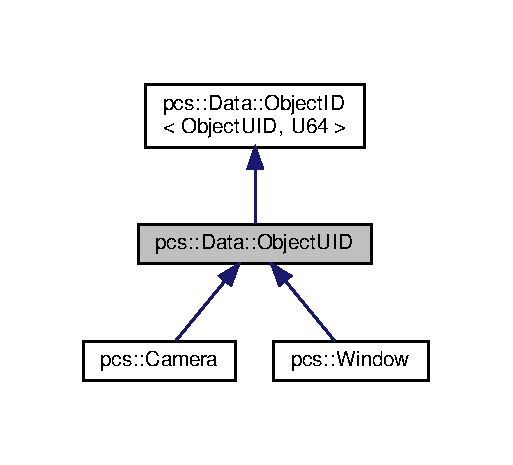
\includegraphics[width=246pt]{classpcs_1_1Data_1_1ObjectUID__inherit__graph}
\end{center}
\end{figure}


Collaboration diagram for pcs\+:\+:Data\+:\+:Object\+U\+ID\+:\nopagebreak
\begin{figure}[H]
\begin{center}
\leavevmode
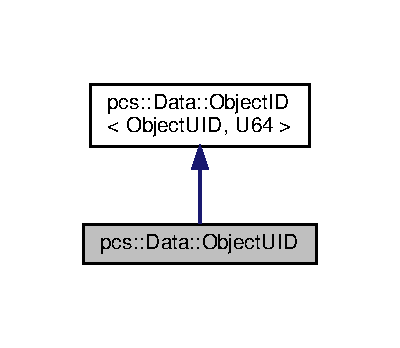
\includegraphics[width=192pt]{classpcs_1_1Data_1_1ObjectUID__coll__graph}
\end{center}
\end{figure}
\subsection*{Public Member Functions}
\begin{DoxyCompactItemize}
\item 
\hyperlink{classpcs_1_1Data_1_1ObjectUID_a04780c31ec526182ea5abf7351e84459}{Object\+U\+ID} ()
\item 
void \hyperlink{classpcs_1_1Data_1_1ObjectUID_a8ceb01cdc531488d8033f7eeb07cb796}{override\+ID} (\hyperlink{namespacepcs_1_1Data_a9aad6b21cf2fcd3515ecc3bbd069eb34}{U64} uid)
\end{DoxyCompactItemize}
\subsection*{Private Member Functions}
\begin{DoxyCompactItemize}
\item 
\hyperlink{namespacepcs_1_1Data_a9aad6b21cf2fcd3515ecc3bbd069eb34}{U64} \hyperlink{classpcs_1_1Data_1_1ObjectUID_a1a1cc75b0ed7e6c04f2f5daa33e0193e}{get\+Next} () override
\begin{DoxyCompactList}\small\item\em Get the next ID. \end{DoxyCompactList}\end{DoxyCompactItemize}
\subsection*{Additional Inherited Members}


\subsection{Constructor \& Destructor Documentation}
\mbox{\Hypertarget{classpcs_1_1Data_1_1ObjectUID_a04780c31ec526182ea5abf7351e84459}\label{classpcs_1_1Data_1_1ObjectUID_a04780c31ec526182ea5abf7351e84459}} 
\index{pcs\+::\+Data\+::\+Object\+U\+ID@{pcs\+::\+Data\+::\+Object\+U\+ID}!Object\+U\+ID@{Object\+U\+ID}}
\index{Object\+U\+ID@{Object\+U\+ID}!pcs\+::\+Data\+::\+Object\+U\+ID@{pcs\+::\+Data\+::\+Object\+U\+ID}}
\subsubsection{\texorpdfstring{Object\+U\+I\+D()}{ObjectUID()}}
{\footnotesize\ttfamily pcs\+::\+Data\+::\+Object\+U\+I\+D\+::\+Object\+U\+ID (\begin{DoxyParamCaption}{ }\end{DoxyParamCaption})\hspace{0.3cm}{\ttfamily [inline]}}



\subsection{Member Function Documentation}
\mbox{\Hypertarget{classpcs_1_1Data_1_1ObjectUID_a1a1cc75b0ed7e6c04f2f5daa33e0193e}\label{classpcs_1_1Data_1_1ObjectUID_a1a1cc75b0ed7e6c04f2f5daa33e0193e}} 
\index{pcs\+::\+Data\+::\+Object\+U\+ID@{pcs\+::\+Data\+::\+Object\+U\+ID}!get\+Next@{get\+Next}}
\index{get\+Next@{get\+Next}!pcs\+::\+Data\+::\+Object\+U\+ID@{pcs\+::\+Data\+::\+Object\+U\+ID}}
\subsubsection{\texorpdfstring{get\+Next()}{getNext()}}
{\footnotesize\ttfamily \hyperlink{namespacepcs_1_1Data_a9aad6b21cf2fcd3515ecc3bbd069eb34}{U64} pcs\+::\+Data\+::\+Object\+U\+I\+D\+::get\+Next (\begin{DoxyParamCaption}{ }\end{DoxyParamCaption})\hspace{0.3cm}{\ttfamily [inline]}, {\ttfamily [override]}, {\ttfamily [private]}, {\ttfamily [virtual]}}



Get the next ID. 

\begin{DoxyReturn}{Returns}
unsigned int Incremented ID 
\end{DoxyReturn}


Reimplemented from \hyperlink{classpcs_1_1Data_1_1ObjectID_a01456dc5ee820984c83c089e413255ec}{pcs\+::\+Data\+::\+Object\+I\+D$<$ Object\+U\+I\+D, U64 $>$}.

\mbox{\Hypertarget{classpcs_1_1Data_1_1ObjectUID_a8ceb01cdc531488d8033f7eeb07cb796}\label{classpcs_1_1Data_1_1ObjectUID_a8ceb01cdc531488d8033f7eeb07cb796}} 
\index{pcs\+::\+Data\+::\+Object\+U\+ID@{pcs\+::\+Data\+::\+Object\+U\+ID}!override\+ID@{override\+ID}}
\index{override\+ID@{override\+ID}!pcs\+::\+Data\+::\+Object\+U\+ID@{pcs\+::\+Data\+::\+Object\+U\+ID}}
\subsubsection{\texorpdfstring{override\+I\+D()}{overrideID()}}
{\footnotesize\ttfamily void pcs\+::\+Data\+::\+Object\+U\+I\+D\+::override\+ID (\begin{DoxyParamCaption}\item[{\hyperlink{namespacepcs_1_1Data_a9aad6b21cf2fcd3515ecc3bbd069eb34}{U64}}]{uid }\end{DoxyParamCaption})\hspace{0.3cm}{\ttfamily [inline]}}



The documentation for this class was generated from the following file\+:\begin{DoxyCompactItemize}
\item 
include/\+Perceus/\+Data/\hyperlink{ObjectID_8h}{Object\+I\+D.\+h}\end{DoxyCompactItemize}

\hypertarget{classpcs_1_1ParserOBJ}{}\section{pcs\+:\+:Parser\+O\+BJ Class Reference}
\label{classpcs_1_1ParserOBJ}\index{pcs\+::\+Parser\+O\+BJ@{pcs\+::\+Parser\+O\+BJ}}


{\ttfamily \#include $<$Parser\+O\+B\+J.\+h$>$}



Inheritance diagram for pcs\+:\+:Parser\+O\+BJ\+:\nopagebreak
\begin{figure}[H]
\begin{center}
\leavevmode
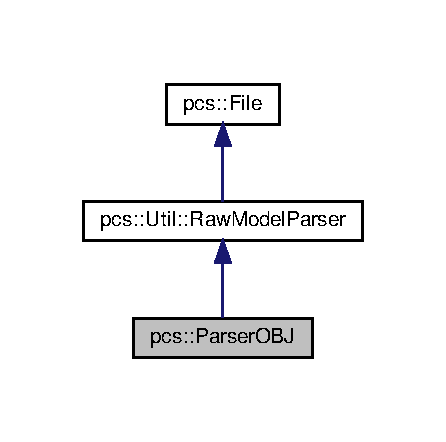
\includegraphics[width=214pt]{classpcs_1_1ParserOBJ__inherit__graph}
\end{center}
\end{figure}


Collaboration diagram for pcs\+:\+:Parser\+O\+BJ\+:\nopagebreak
\begin{figure}[H]
\begin{center}
\leavevmode
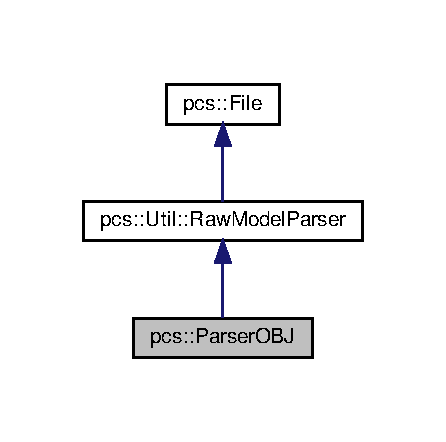
\includegraphics[width=214pt]{classpcs_1_1ParserOBJ__coll__graph}
\end{center}
\end{figure}
\subsection*{Public Member Functions}
\begin{DoxyCompactItemize}
\item 
\hyperlink{classpcs_1_1VertexArray}{Vertex\+Array} $\ast$ \hyperlink{classpcs_1_1ParserOBJ_a9f83ac259feacf8ab83bfd73dc3ebb62}{parse\+File} () const override
\end{DoxyCompactItemize}
\subsection*{Additional Inherited Members}


\subsection{Member Function Documentation}
\mbox{\Hypertarget{classpcs_1_1ParserOBJ_a9f83ac259feacf8ab83bfd73dc3ebb62}\label{classpcs_1_1ParserOBJ_a9f83ac259feacf8ab83bfd73dc3ebb62}} 
\index{pcs\+::\+Parser\+O\+BJ@{pcs\+::\+Parser\+O\+BJ}!parse\+File@{parse\+File}}
\index{parse\+File@{parse\+File}!pcs\+::\+Parser\+O\+BJ@{pcs\+::\+Parser\+O\+BJ}}
\subsubsection{\texorpdfstring{parse\+File()}{parseFile()}}
{\footnotesize\ttfamily \hyperlink{classpcs_1_1VertexArray}{Vertex\+Array} $\ast$ pcs\+::\+Parser\+O\+B\+J\+::parse\+File (\begin{DoxyParamCaption}{ }\end{DoxyParamCaption}) const\hspace{0.3cm}{\ttfamily [override]}, {\ttfamily [virtual]}}



Implements \hyperlink{classpcs_1_1Util_1_1RawModelParser_a8f14c3221db14dc46ef6c8858690e106}{pcs\+::\+Util\+::\+Raw\+Model\+Parser}.



The documentation for this class was generated from the following files\+:\begin{DoxyCompactItemize}
\item 
include/\+Perceus/\+Util/\+Parser/\hyperlink{ParserOBJ_8h}{Parser\+O\+B\+J.\+h}\item 
src/\+Util/\+Parser/\hyperlink{ParserOBJ_8cpp}{Parser\+O\+B\+J.\+cpp}\end{DoxyCompactItemize}

\hypertarget{classpcs_1_1RawModel}{}\section{pcs\+:\+:Raw\+Model Class Reference}
\label{classpcs_1_1RawModel}\index{pcs\+::\+Raw\+Model@{pcs\+::\+Raw\+Model}}


{\ttfamily \#include $<$Raw\+Model.\+h$>$}



Inheritance diagram for pcs\+:\+:Raw\+Model\+:\nopagebreak
\begin{figure}[H]
\begin{center}
\leavevmode
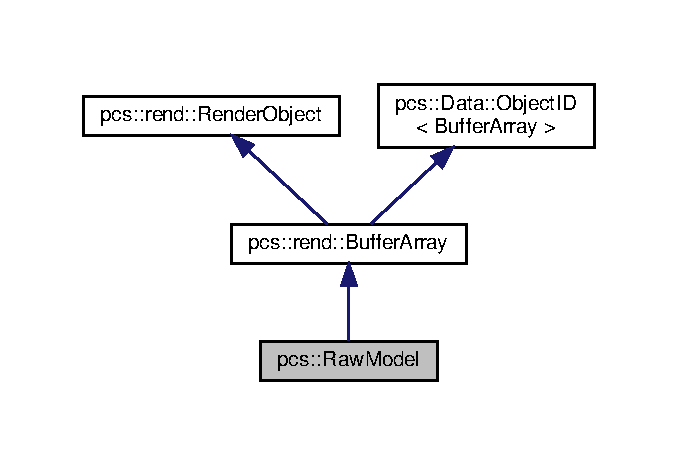
\includegraphics[width=326pt]{classpcs_1_1RawModel__inherit__graph}
\end{center}
\end{figure}


Collaboration diagram for pcs\+:\+:Raw\+Model\+:\nopagebreak
\begin{figure}[H]
\begin{center}
\leavevmode
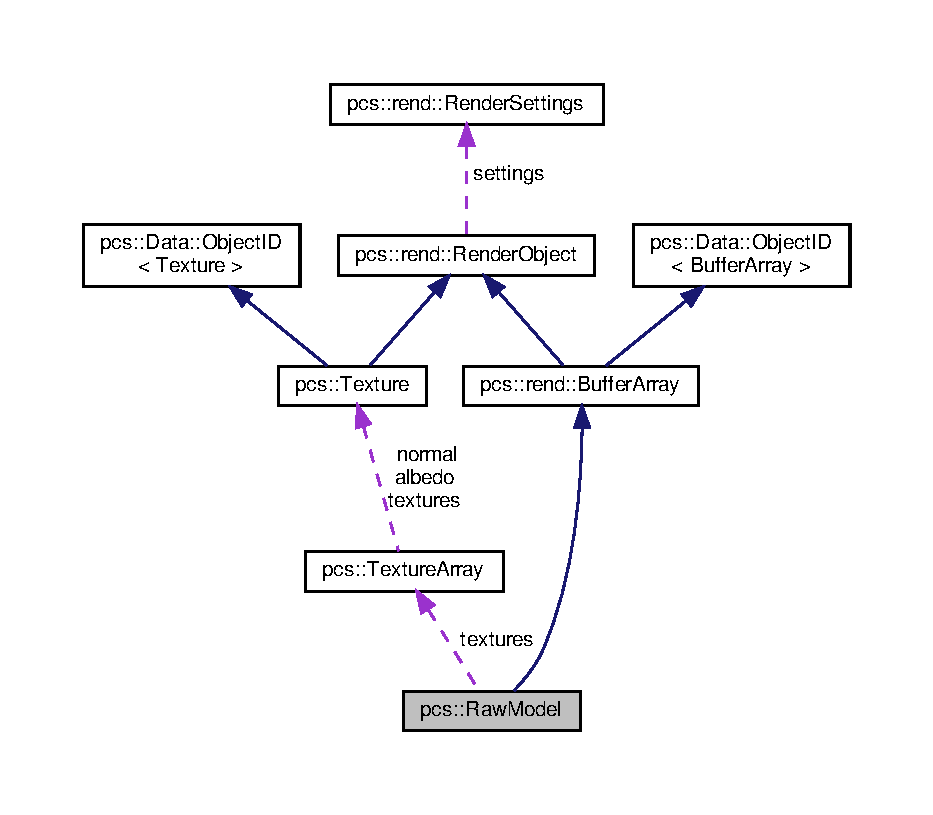
\includegraphics[width=350pt]{classpcs_1_1RawModel__coll__graph}
\end{center}
\end{figure}
\subsection*{Public Member Functions}
\begin{DoxyCompactItemize}
\item 
\hyperlink{classpcs_1_1RawModel_a79a06ab99e5e7438ad61c68601e9e7ea}{Raw\+Model} ()
\item 
\hyperlink{classpcs_1_1RawModel_addb04fed9a364e9c24b8b4f4b69480a7}{Raw\+Model} (const \hyperlink{classpcs_1_1VertexArray}{Vertex\+Array} \&vertex)
\item 
\hyperlink{classpcs_1_1RawModel_a3fb7c140b100311f737d23dfb9fbf6d6}{$\sim$\+Raw\+Model} ()
\item 
\hyperlink{unionpcs_1_1TextureArray}{Texture\+Array} \& \hyperlink{classpcs_1_1RawModel_a3caaf1aa1419660fcd4c33807eb96782}{get\+Textures} ()
\item 
bool \hyperlink{classpcs_1_1RawModel_ae62c8b9e99a8d83c79338b86bd857f0d}{load\+Colors} (std\+::vector$<$ \hyperlink{structpcs_1_1Color}{Color} $>$ colors)
\item 
bool \hyperlink{classpcs_1_1RawModel_add81afbd701da03693bbb45921425b9f}{load\+Normals} (std\+::vector$<$ \hyperlink{namespacepcs_a68e0f517680976c17c810ffe6952cbab}{Vec3f} $>$ normals)
\item 
bool \hyperlink{classpcs_1_1RawModel_ac87cd0d4a1bd6d587b9e680f02a810c3}{load\+Vertices} (std\+::vector$<$ \hyperlink{namespacepcs_a68e0f517680976c17c810ffe6952cbab}{Vec3f} $>$ vertices)
\item 
bool \hyperlink{classpcs_1_1RawModel_af33dad372a9f74e01ef8412e805d99cf}{load\+Tex\+Coords} (std\+::vector$<$ \hyperlink{namespacepcs_a4b2fd718bd0800b6aa492b1c60f19edc}{Vec2f} $>$ tex\+Coords)
\item 
bool \hyperlink{classpcs_1_1RawModel_acf35bf470e0ca38f98a53a7db7fa0a3b}{load\+Model\+Matrices} (std\+::vector$<$ \hyperlink{structpcs_1_1Mat4f}{Mat4f} $>$ \&matrices)
\item 
bool \hyperlink{classpcs_1_1RawModel_a64c1634cbeb22fc4b087f24cac6ba242}{load\+Bitangents} (std\+::vector$<$ \hyperlink{namespacepcs_a68e0f517680976c17c810ffe6952cbab}{Vec3f} $>$ bitangents)
\item 
bool \hyperlink{classpcs_1_1RawModel_ad1f5e752490cbba94a639b49cbd08c93}{load\+Tangents} (std\+::vector$<$ \hyperlink{namespacepcs_a68e0f517680976c17c810ffe6952cbab}{Vec3f} $>$ tangents)
\item 
bool \hyperlink{classpcs_1_1RawModel_a147fb1b196e18e2f2deb1a6e86fff9b6}{generate\+Indices} (std\+::vector$<$ \hyperlink{namespacepcs_a68e0f517680976c17c810ffe6952cbab}{Vec3f} $>$ vertices)
\end{DoxyCompactItemize}
\subsection*{Private Attributes}
\begin{DoxyCompactItemize}
\item 
\hyperlink{unionpcs_1_1TextureArray}{Texture\+Array} \hyperlink{classpcs_1_1RawModel_a5441811d19297669eefdb405ea94ce0c}{textures}
\end{DoxyCompactItemize}
\subsection*{Additional Inherited Members}


\subsection{Constructor \& Destructor Documentation}
\mbox{\Hypertarget{classpcs_1_1RawModel_a79a06ab99e5e7438ad61c68601e9e7ea}\label{classpcs_1_1RawModel_a79a06ab99e5e7438ad61c68601e9e7ea}} 
\index{pcs\+::\+Raw\+Model@{pcs\+::\+Raw\+Model}!Raw\+Model@{Raw\+Model}}
\index{Raw\+Model@{Raw\+Model}!pcs\+::\+Raw\+Model@{pcs\+::\+Raw\+Model}}
\subsubsection{\texorpdfstring{Raw\+Model()}{RawModel()}\hspace{0.1cm}{\footnotesize\ttfamily [1/2]}}
{\footnotesize\ttfamily pcs\+::\+Raw\+Model\+::\+Raw\+Model (\begin{DoxyParamCaption}{ }\end{DoxyParamCaption})\hspace{0.3cm}{\ttfamily [inline]}}

\mbox{\Hypertarget{classpcs_1_1RawModel_addb04fed9a364e9c24b8b4f4b69480a7}\label{classpcs_1_1RawModel_addb04fed9a364e9c24b8b4f4b69480a7}} 
\index{pcs\+::\+Raw\+Model@{pcs\+::\+Raw\+Model}!Raw\+Model@{Raw\+Model}}
\index{Raw\+Model@{Raw\+Model}!pcs\+::\+Raw\+Model@{pcs\+::\+Raw\+Model}}
\subsubsection{\texorpdfstring{Raw\+Model()}{RawModel()}\hspace{0.1cm}{\footnotesize\ttfamily [2/2]}}
{\footnotesize\ttfamily pcs\+::\+Raw\+Model\+::\+Raw\+Model (\begin{DoxyParamCaption}\item[{const \hyperlink{classpcs_1_1VertexArray}{Vertex\+Array} \&}]{vertex }\end{DoxyParamCaption})}

\mbox{\Hypertarget{classpcs_1_1RawModel_a3fb7c140b100311f737d23dfb9fbf6d6}\label{classpcs_1_1RawModel_a3fb7c140b100311f737d23dfb9fbf6d6}} 
\index{pcs\+::\+Raw\+Model@{pcs\+::\+Raw\+Model}!````~Raw\+Model@{$\sim$\+Raw\+Model}}
\index{````~Raw\+Model@{$\sim$\+Raw\+Model}!pcs\+::\+Raw\+Model@{pcs\+::\+Raw\+Model}}
\subsubsection{\texorpdfstring{$\sim$\+Raw\+Model()}{~RawModel()}}
{\footnotesize\ttfamily pcs\+::\+Raw\+Model\+::$\sim$\+Raw\+Model (\begin{DoxyParamCaption}{ }\end{DoxyParamCaption})}



\subsection{Member Function Documentation}
\mbox{\Hypertarget{classpcs_1_1RawModel_a147fb1b196e18e2f2deb1a6e86fff9b6}\label{classpcs_1_1RawModel_a147fb1b196e18e2f2deb1a6e86fff9b6}} 
\index{pcs\+::\+Raw\+Model@{pcs\+::\+Raw\+Model}!generate\+Indices@{generate\+Indices}}
\index{generate\+Indices@{generate\+Indices}!pcs\+::\+Raw\+Model@{pcs\+::\+Raw\+Model}}
\subsubsection{\texorpdfstring{generate\+Indices()}{generateIndices()}}
{\footnotesize\ttfamily bool pcs\+::\+Raw\+Model\+::generate\+Indices (\begin{DoxyParamCaption}\item[{std\+::vector$<$ \hyperlink{namespacepcs_a68e0f517680976c17c810ffe6952cbab}{Vec3f} $>$}]{vertices }\end{DoxyParamCaption})}

\mbox{\Hypertarget{classpcs_1_1RawModel_a3caaf1aa1419660fcd4c33807eb96782}\label{classpcs_1_1RawModel_a3caaf1aa1419660fcd4c33807eb96782}} 
\index{pcs\+::\+Raw\+Model@{pcs\+::\+Raw\+Model}!get\+Textures@{get\+Textures}}
\index{get\+Textures@{get\+Textures}!pcs\+::\+Raw\+Model@{pcs\+::\+Raw\+Model}}
\subsubsection{\texorpdfstring{get\+Textures()}{getTextures()}}
{\footnotesize\ttfamily \hyperlink{unionpcs_1_1TextureArray}{Texture\+Array}\& pcs\+::\+Raw\+Model\+::get\+Textures (\begin{DoxyParamCaption}{ }\end{DoxyParamCaption})\hspace{0.3cm}{\ttfamily [inline]}}

\mbox{\Hypertarget{classpcs_1_1RawModel_a64c1634cbeb22fc4b087f24cac6ba242}\label{classpcs_1_1RawModel_a64c1634cbeb22fc4b087f24cac6ba242}} 
\index{pcs\+::\+Raw\+Model@{pcs\+::\+Raw\+Model}!load\+Bitangents@{load\+Bitangents}}
\index{load\+Bitangents@{load\+Bitangents}!pcs\+::\+Raw\+Model@{pcs\+::\+Raw\+Model}}
\subsubsection{\texorpdfstring{load\+Bitangents()}{loadBitangents()}}
{\footnotesize\ttfamily bool pcs\+::\+Raw\+Model\+::load\+Bitangents (\begin{DoxyParamCaption}\item[{std\+::vector$<$ \hyperlink{namespacepcs_a68e0f517680976c17c810ffe6952cbab}{Vec3f} $>$}]{bitangents }\end{DoxyParamCaption})}

\mbox{\Hypertarget{classpcs_1_1RawModel_ae62c8b9e99a8d83c79338b86bd857f0d}\label{classpcs_1_1RawModel_ae62c8b9e99a8d83c79338b86bd857f0d}} 
\index{pcs\+::\+Raw\+Model@{pcs\+::\+Raw\+Model}!load\+Colors@{load\+Colors}}
\index{load\+Colors@{load\+Colors}!pcs\+::\+Raw\+Model@{pcs\+::\+Raw\+Model}}
\subsubsection{\texorpdfstring{load\+Colors()}{loadColors()}}
{\footnotesize\ttfamily bool pcs\+::\+Raw\+Model\+::load\+Colors (\begin{DoxyParamCaption}\item[{std\+::vector$<$ \hyperlink{structpcs_1_1Color}{Color} $>$}]{colors }\end{DoxyParamCaption})}

\mbox{\Hypertarget{classpcs_1_1RawModel_acf35bf470e0ca38f98a53a7db7fa0a3b}\label{classpcs_1_1RawModel_acf35bf470e0ca38f98a53a7db7fa0a3b}} 
\index{pcs\+::\+Raw\+Model@{pcs\+::\+Raw\+Model}!load\+Model\+Matrices@{load\+Model\+Matrices}}
\index{load\+Model\+Matrices@{load\+Model\+Matrices}!pcs\+::\+Raw\+Model@{pcs\+::\+Raw\+Model}}
\subsubsection{\texorpdfstring{load\+Model\+Matrices()}{loadModelMatrices()}}
{\footnotesize\ttfamily bool pcs\+::\+Raw\+Model\+::load\+Model\+Matrices (\begin{DoxyParamCaption}\item[{std\+::vector$<$ \hyperlink{structpcs_1_1Mat4f}{Mat4f} $>$ \&}]{matrices }\end{DoxyParamCaption})}

\mbox{\Hypertarget{classpcs_1_1RawModel_add81afbd701da03693bbb45921425b9f}\label{classpcs_1_1RawModel_add81afbd701da03693bbb45921425b9f}} 
\index{pcs\+::\+Raw\+Model@{pcs\+::\+Raw\+Model}!load\+Normals@{load\+Normals}}
\index{load\+Normals@{load\+Normals}!pcs\+::\+Raw\+Model@{pcs\+::\+Raw\+Model}}
\subsubsection{\texorpdfstring{load\+Normals()}{loadNormals()}}
{\footnotesize\ttfamily bool pcs\+::\+Raw\+Model\+::load\+Normals (\begin{DoxyParamCaption}\item[{std\+::vector$<$ \hyperlink{namespacepcs_a68e0f517680976c17c810ffe6952cbab}{Vec3f} $>$}]{normals }\end{DoxyParamCaption})}

\mbox{\Hypertarget{classpcs_1_1RawModel_ad1f5e752490cbba94a639b49cbd08c93}\label{classpcs_1_1RawModel_ad1f5e752490cbba94a639b49cbd08c93}} 
\index{pcs\+::\+Raw\+Model@{pcs\+::\+Raw\+Model}!load\+Tangents@{load\+Tangents}}
\index{load\+Tangents@{load\+Tangents}!pcs\+::\+Raw\+Model@{pcs\+::\+Raw\+Model}}
\subsubsection{\texorpdfstring{load\+Tangents()}{loadTangents()}}
{\footnotesize\ttfamily bool pcs\+::\+Raw\+Model\+::load\+Tangents (\begin{DoxyParamCaption}\item[{std\+::vector$<$ \hyperlink{namespacepcs_a68e0f517680976c17c810ffe6952cbab}{Vec3f} $>$}]{tangents }\end{DoxyParamCaption})}

\mbox{\Hypertarget{classpcs_1_1RawModel_af33dad372a9f74e01ef8412e805d99cf}\label{classpcs_1_1RawModel_af33dad372a9f74e01ef8412e805d99cf}} 
\index{pcs\+::\+Raw\+Model@{pcs\+::\+Raw\+Model}!load\+Tex\+Coords@{load\+Tex\+Coords}}
\index{load\+Tex\+Coords@{load\+Tex\+Coords}!pcs\+::\+Raw\+Model@{pcs\+::\+Raw\+Model}}
\subsubsection{\texorpdfstring{load\+Tex\+Coords()}{loadTexCoords()}}
{\footnotesize\ttfamily bool pcs\+::\+Raw\+Model\+::load\+Tex\+Coords (\begin{DoxyParamCaption}\item[{std\+::vector$<$ \hyperlink{namespacepcs_a4b2fd718bd0800b6aa492b1c60f19edc}{Vec2f} $>$}]{tex\+Coords }\end{DoxyParamCaption})}

\mbox{\Hypertarget{classpcs_1_1RawModel_ac87cd0d4a1bd6d587b9e680f02a810c3}\label{classpcs_1_1RawModel_ac87cd0d4a1bd6d587b9e680f02a810c3}} 
\index{pcs\+::\+Raw\+Model@{pcs\+::\+Raw\+Model}!load\+Vertices@{load\+Vertices}}
\index{load\+Vertices@{load\+Vertices}!pcs\+::\+Raw\+Model@{pcs\+::\+Raw\+Model}}
\subsubsection{\texorpdfstring{load\+Vertices()}{loadVertices()}}
{\footnotesize\ttfamily bool pcs\+::\+Raw\+Model\+::load\+Vertices (\begin{DoxyParamCaption}\item[{std\+::vector$<$ \hyperlink{namespacepcs_a68e0f517680976c17c810ffe6952cbab}{Vec3f} $>$}]{vertices }\end{DoxyParamCaption})}



\subsection{Member Data Documentation}
\mbox{\Hypertarget{classpcs_1_1RawModel_a5441811d19297669eefdb405ea94ce0c}\label{classpcs_1_1RawModel_a5441811d19297669eefdb405ea94ce0c}} 
\index{pcs\+::\+Raw\+Model@{pcs\+::\+Raw\+Model}!textures@{textures}}
\index{textures@{textures}!pcs\+::\+Raw\+Model@{pcs\+::\+Raw\+Model}}
\subsubsection{\texorpdfstring{textures}{textures}}
{\footnotesize\ttfamily \hyperlink{unionpcs_1_1TextureArray}{Texture\+Array} pcs\+::\+Raw\+Model\+::textures\hspace{0.3cm}{\ttfamily [private]}}



The documentation for this class was generated from the following files\+:\begin{DoxyCompactItemize}
\item 
include/\+Perceus/\+Core/\+Graphics/\+Entities/\hyperlink{RawModel_8h}{Raw\+Model.\+h}\item 
src/\+Core/\+Graphics/\+Entities/\hyperlink{RawModel_8cpp}{Raw\+Model.\+cpp}\end{DoxyCompactItemize}

\hypertarget{classpcs_1_1Util_1_1RawModelParser}{}\section{pcs\+:\+:Util\+:\+:Raw\+Model\+Parser Class Reference}
\label{classpcs_1_1Util_1_1RawModelParser}\index{pcs\+::\+Util\+::\+Raw\+Model\+Parser@{pcs\+::\+Util\+::\+Raw\+Model\+Parser}}


{\ttfamily \#include $<$Raw\+Model\+Parser.\+h$>$}



Inheritance diagram for pcs\+:\+:Util\+:\+:Raw\+Model\+Parser\+:\nopagebreak
\begin{figure}[H]
\begin{center}
\leavevmode
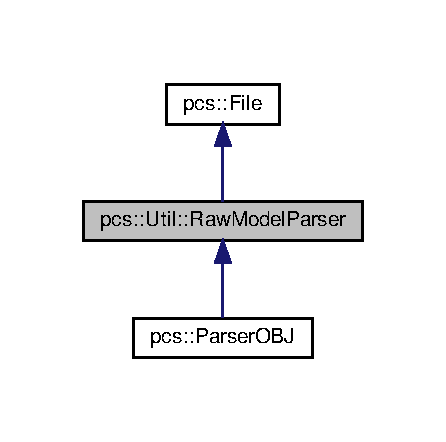
\includegraphics[width=214pt]{classpcs_1_1Util_1_1RawModelParser__inherit__graph}
\end{center}
\end{figure}


Collaboration diagram for pcs\+:\+:Util\+:\+:Raw\+Model\+Parser\+:\nopagebreak
\begin{figure}[H]
\begin{center}
\leavevmode
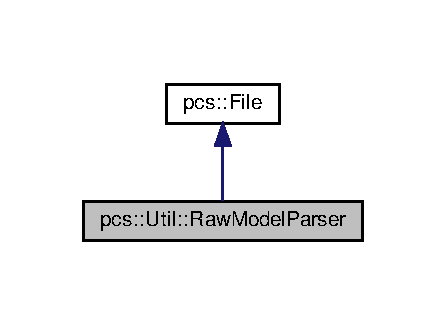
\includegraphics[width=214pt]{classpcs_1_1Util_1_1RawModelParser__coll__graph}
\end{center}
\end{figure}
\subsection*{Public Member Functions}
\begin{DoxyCompactItemize}
\item 
virtual \hyperlink{classpcs_1_1VertexArray}{Vertex\+Array} $\ast$ \hyperlink{classpcs_1_1Util_1_1RawModelParser_a8f14c3221db14dc46ef6c8858690e106}{parse\+File} () const =0
\end{DoxyCompactItemize}
\subsection*{Additional Inherited Members}


\subsection{Member Function Documentation}
\mbox{\Hypertarget{classpcs_1_1Util_1_1RawModelParser_a8f14c3221db14dc46ef6c8858690e106}\label{classpcs_1_1Util_1_1RawModelParser_a8f14c3221db14dc46ef6c8858690e106}} 
\index{pcs\+::\+Util\+::\+Raw\+Model\+Parser@{pcs\+::\+Util\+::\+Raw\+Model\+Parser}!parse\+File@{parse\+File}}
\index{parse\+File@{parse\+File}!pcs\+::\+Util\+::\+Raw\+Model\+Parser@{pcs\+::\+Util\+::\+Raw\+Model\+Parser}}
\subsubsection{\texorpdfstring{parse\+File()}{parseFile()}}
{\footnotesize\ttfamily virtual \hyperlink{classpcs_1_1VertexArray}{Vertex\+Array}$\ast$ pcs\+::\+Util\+::\+Raw\+Model\+Parser\+::parse\+File (\begin{DoxyParamCaption}{ }\end{DoxyParamCaption}) const\hspace{0.3cm}{\ttfamily [pure virtual]}}



Implemented in \hyperlink{classpcs_1_1ParserOBJ_a9f83ac259feacf8ab83bfd73dc3ebb62}{pcs\+::\+Parser\+O\+BJ}.



The documentation for this class was generated from the following file\+:\begin{DoxyCompactItemize}
\item 
include/\+Perceus/\+Util/\+Parser/\hyperlink{RawModelParser_8h}{Raw\+Model\+Parser.\+h}\end{DoxyCompactItemize}

\hypertarget{classpcs_1_1Util_1_1Mem_1_1RegTable}{}\section{pcs\+:\+:Util\+:\+:Mem\+:\+:Reg\+Table Class Reference}
\label{classpcs_1_1Util_1_1Mem_1_1RegTable}\index{pcs\+::\+Util\+::\+Mem\+::\+Reg\+Table@{pcs\+::\+Util\+::\+Mem\+::\+Reg\+Table}}


{\ttfamily \#include $<$Reg\+Table.\+h$>$}



Inheritance diagram for pcs\+:\+:Util\+:\+:Mem\+:\+:Reg\+Table\+:\nopagebreak
\begin{figure}[H]
\begin{center}
\leavevmode
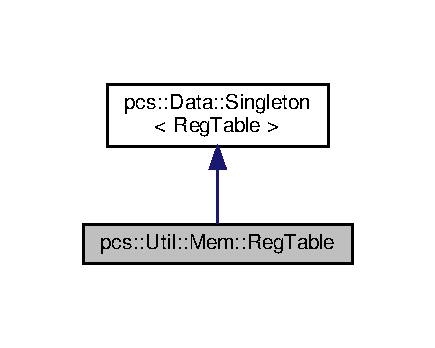
\includegraphics[width=209pt]{classpcs_1_1Util_1_1Mem_1_1RegTable__inherit__graph}
\end{center}
\end{figure}


Collaboration diagram for pcs\+:\+:Util\+:\+:Mem\+:\+:Reg\+Table\+:\nopagebreak
\begin{figure}[H]
\begin{center}
\leavevmode
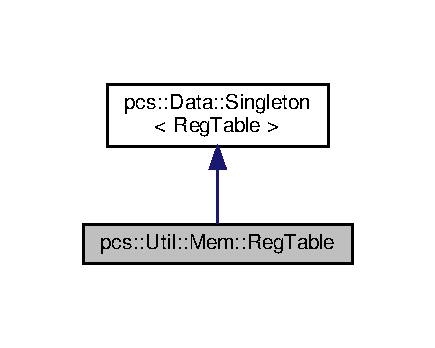
\includegraphics[width=209pt]{classpcs_1_1Util_1_1Mem_1_1RegTable__coll__graph}
\end{center}
\end{figure}
\subsection*{Public Member Functions}
\begin{DoxyCompactItemize}
\item 
\hyperlink{classpcs_1_1Util_1_1Mem_1_1RegTable_abf5ce566d2af0fa1267ff19e24bf8912}{Reg\+Table} ()
\item 
\hyperlink{classpcs_1_1Util_1_1Mem_1_1RegTable_a665bb13c8159497d6ccf30aefb525681}{Reg\+Table} (const \hyperlink{classpcs_1_1Util_1_1Mem_1_1RegTable}{Reg\+Table} \&)=delete
\item 
\hyperlink{classpcs_1_1Util_1_1Mem_1_1RegTable}{Reg\+Table} \& \hyperlink{classpcs_1_1Util_1_1Mem_1_1RegTable_ae4147c2cb9b26272879b73330eba0908}{operator=} (const \hyperlink{classpcs_1_1Util_1_1Mem_1_1RegTable}{Reg\+Table} \&)=delete
\item 
{\footnotesize template$<$typename T $>$ }\\T $\ast$ \hyperlink{classpcs_1_1Util_1_1Mem_1_1RegTable_ae343c69786a6b7fcfdff6d311a18c50f}{collect} (\hyperlink{namespacepcs_1_1Util_1_1Mem_ab390aefcd13d26db4db397b784b4b9c6}{U64} uid)
\item 
{\footnotesize template$<$typename T $>$ }\\void \hyperlink{classpcs_1_1Util_1_1Mem_1_1RegTable_a3e527aef5808d02522f2e1ab27fb6947}{register\+Object} (\hyperlink{namespacepcs_1_1Util_1_1Mem_ab390aefcd13d26db4db397b784b4b9c6}{U64} uid, const T $\ast$obj)
\item 
{\footnotesize template$<$typename T $>$ }\\void \hyperlink{classpcs_1_1Util_1_1Mem_1_1RegTable_a7a6caf2a5c20e8b28a8f454cc91aa96e}{register\+Object} (\hyperlink{namespacepcs_1_1Util_1_1Mem_ab390aefcd13d26db4db397b784b4b9c6}{U64} uid, const T \&obj)
\end{DoxyCompactItemize}
\subsection*{Private Member Functions}
\begin{DoxyCompactItemize}
\item 
void \hyperlink{classpcs_1_1Util_1_1Mem_1_1RegTable_acd1220bca68b300651daccd808140707}{register\+Data\+Point} (\hyperlink{namespacepcs_1_1Util_1_1Mem_ab390aefcd13d26db4db397b784b4b9c6}{U64} uid, \hyperlink{structpcs_1_1Util_1_1Mem_1_1DataPoint}{Data\+Point} data)
\end{DoxyCompactItemize}
\subsection*{Private Attributes}
\begin{DoxyCompactItemize}
\item 
std\+::unordered\+\_\+map$<$ \hyperlink{namespacepcs_1_1Util_1_1Mem_ab390aefcd13d26db4db397b784b4b9c6}{U64}, \hyperlink{structpcs_1_1Util_1_1Mem_1_1DataPoint}{Data\+Point} $>$ \hyperlink{classpcs_1_1Util_1_1Mem_1_1RegTable_a00dba5deb5b8f0b1ce83dc1f90a2187f}{table}
\end{DoxyCompactItemize}
\subsection*{Additional Inherited Members}


\subsection{Constructor \& Destructor Documentation}
\mbox{\Hypertarget{classpcs_1_1Util_1_1Mem_1_1RegTable_abf5ce566d2af0fa1267ff19e24bf8912}\label{classpcs_1_1Util_1_1Mem_1_1RegTable_abf5ce566d2af0fa1267ff19e24bf8912}} 
\index{pcs\+::\+Util\+::\+Mem\+::\+Reg\+Table@{pcs\+::\+Util\+::\+Mem\+::\+Reg\+Table}!Reg\+Table@{Reg\+Table}}
\index{Reg\+Table@{Reg\+Table}!pcs\+::\+Util\+::\+Mem\+::\+Reg\+Table@{pcs\+::\+Util\+::\+Mem\+::\+Reg\+Table}}
\subsubsection{\texorpdfstring{Reg\+Table()}{RegTable()}\hspace{0.1cm}{\footnotesize\ttfamily [1/2]}}
{\footnotesize\ttfamily pcs\+::\+Util\+::\+Mem\+::\+Reg\+Table\+::\+Reg\+Table (\begin{DoxyParamCaption}{ }\end{DoxyParamCaption})\hspace{0.3cm}{\ttfamily [inline]}}

\mbox{\Hypertarget{classpcs_1_1Util_1_1Mem_1_1RegTable_a665bb13c8159497d6ccf30aefb525681}\label{classpcs_1_1Util_1_1Mem_1_1RegTable_a665bb13c8159497d6ccf30aefb525681}} 
\index{pcs\+::\+Util\+::\+Mem\+::\+Reg\+Table@{pcs\+::\+Util\+::\+Mem\+::\+Reg\+Table}!Reg\+Table@{Reg\+Table}}
\index{Reg\+Table@{Reg\+Table}!pcs\+::\+Util\+::\+Mem\+::\+Reg\+Table@{pcs\+::\+Util\+::\+Mem\+::\+Reg\+Table}}
\subsubsection{\texorpdfstring{Reg\+Table()}{RegTable()}\hspace{0.1cm}{\footnotesize\ttfamily [2/2]}}
{\footnotesize\ttfamily pcs\+::\+Util\+::\+Mem\+::\+Reg\+Table\+::\+Reg\+Table (\begin{DoxyParamCaption}\item[{const \hyperlink{classpcs_1_1Util_1_1Mem_1_1RegTable}{Reg\+Table} \&}]{ }\end{DoxyParamCaption})\hspace{0.3cm}{\ttfamily [delete]}}



\subsection{Member Function Documentation}
\mbox{\Hypertarget{classpcs_1_1Util_1_1Mem_1_1RegTable_ae343c69786a6b7fcfdff6d311a18c50f}\label{classpcs_1_1Util_1_1Mem_1_1RegTable_ae343c69786a6b7fcfdff6d311a18c50f}} 
\index{pcs\+::\+Util\+::\+Mem\+::\+Reg\+Table@{pcs\+::\+Util\+::\+Mem\+::\+Reg\+Table}!collect@{collect}}
\index{collect@{collect}!pcs\+::\+Util\+::\+Mem\+::\+Reg\+Table@{pcs\+::\+Util\+::\+Mem\+::\+Reg\+Table}}
\subsubsection{\texorpdfstring{collect()}{collect()}}
{\footnotesize\ttfamily template$<$typename T $>$ \\
T$\ast$ pcs\+::\+Util\+::\+Mem\+::\+Reg\+Table\+::collect (\begin{DoxyParamCaption}\item[{\hyperlink{namespacepcs_1_1Util_1_1Mem_ab390aefcd13d26db4db397b784b4b9c6}{U64}}]{uid }\end{DoxyParamCaption})\hspace{0.3cm}{\ttfamily [inline]}}

\mbox{\Hypertarget{classpcs_1_1Util_1_1Mem_1_1RegTable_ae4147c2cb9b26272879b73330eba0908}\label{classpcs_1_1Util_1_1Mem_1_1RegTable_ae4147c2cb9b26272879b73330eba0908}} 
\index{pcs\+::\+Util\+::\+Mem\+::\+Reg\+Table@{pcs\+::\+Util\+::\+Mem\+::\+Reg\+Table}!operator=@{operator=}}
\index{operator=@{operator=}!pcs\+::\+Util\+::\+Mem\+::\+Reg\+Table@{pcs\+::\+Util\+::\+Mem\+::\+Reg\+Table}}
\subsubsection{\texorpdfstring{operator=()}{operator=()}}
{\footnotesize\ttfamily \hyperlink{classpcs_1_1Util_1_1Mem_1_1RegTable}{Reg\+Table}\& pcs\+::\+Util\+::\+Mem\+::\+Reg\+Table\+::operator= (\begin{DoxyParamCaption}\item[{const \hyperlink{classpcs_1_1Util_1_1Mem_1_1RegTable}{Reg\+Table} \&}]{ }\end{DoxyParamCaption})\hspace{0.3cm}{\ttfamily [delete]}}

\mbox{\Hypertarget{classpcs_1_1Util_1_1Mem_1_1RegTable_acd1220bca68b300651daccd808140707}\label{classpcs_1_1Util_1_1Mem_1_1RegTable_acd1220bca68b300651daccd808140707}} 
\index{pcs\+::\+Util\+::\+Mem\+::\+Reg\+Table@{pcs\+::\+Util\+::\+Mem\+::\+Reg\+Table}!register\+Data\+Point@{register\+Data\+Point}}
\index{register\+Data\+Point@{register\+Data\+Point}!pcs\+::\+Util\+::\+Mem\+::\+Reg\+Table@{pcs\+::\+Util\+::\+Mem\+::\+Reg\+Table}}
\subsubsection{\texorpdfstring{register\+Data\+Point()}{registerDataPoint()}}
{\footnotesize\ttfamily void pcs\+::\+Util\+::\+Mem\+::\+Reg\+Table\+::register\+Data\+Point (\begin{DoxyParamCaption}\item[{\hyperlink{namespacepcs_1_1Util_1_1Mem_ab390aefcd13d26db4db397b784b4b9c6}{U64}}]{uid,  }\item[{\hyperlink{structpcs_1_1Util_1_1Mem_1_1DataPoint}{Data\+Point}}]{data }\end{DoxyParamCaption})\hspace{0.3cm}{\ttfamily [inline]}, {\ttfamily [private]}}

\mbox{\Hypertarget{classpcs_1_1Util_1_1Mem_1_1RegTable_a3e527aef5808d02522f2e1ab27fb6947}\label{classpcs_1_1Util_1_1Mem_1_1RegTable_a3e527aef5808d02522f2e1ab27fb6947}} 
\index{pcs\+::\+Util\+::\+Mem\+::\+Reg\+Table@{pcs\+::\+Util\+::\+Mem\+::\+Reg\+Table}!register\+Object@{register\+Object}}
\index{register\+Object@{register\+Object}!pcs\+::\+Util\+::\+Mem\+::\+Reg\+Table@{pcs\+::\+Util\+::\+Mem\+::\+Reg\+Table}}
\subsubsection{\texorpdfstring{register\+Object()}{registerObject()}\hspace{0.1cm}{\footnotesize\ttfamily [1/2]}}
{\footnotesize\ttfamily template$<$typename T $>$ \\
void pcs\+::\+Util\+::\+Mem\+::\+Reg\+Table\+::register\+Object (\begin{DoxyParamCaption}\item[{\hyperlink{namespacepcs_1_1Util_1_1Mem_ab390aefcd13d26db4db397b784b4b9c6}{U64}}]{uid,  }\item[{const T $\ast$}]{obj }\end{DoxyParamCaption})\hspace{0.3cm}{\ttfamily [inline]}}

\mbox{\Hypertarget{classpcs_1_1Util_1_1Mem_1_1RegTable_a7a6caf2a5c20e8b28a8f454cc91aa96e}\label{classpcs_1_1Util_1_1Mem_1_1RegTable_a7a6caf2a5c20e8b28a8f454cc91aa96e}} 
\index{pcs\+::\+Util\+::\+Mem\+::\+Reg\+Table@{pcs\+::\+Util\+::\+Mem\+::\+Reg\+Table}!register\+Object@{register\+Object}}
\index{register\+Object@{register\+Object}!pcs\+::\+Util\+::\+Mem\+::\+Reg\+Table@{pcs\+::\+Util\+::\+Mem\+::\+Reg\+Table}}
\subsubsection{\texorpdfstring{register\+Object()}{registerObject()}\hspace{0.1cm}{\footnotesize\ttfamily [2/2]}}
{\footnotesize\ttfamily template$<$typename T $>$ \\
void pcs\+::\+Util\+::\+Mem\+::\+Reg\+Table\+::register\+Object (\begin{DoxyParamCaption}\item[{\hyperlink{namespacepcs_1_1Util_1_1Mem_ab390aefcd13d26db4db397b784b4b9c6}{U64}}]{uid,  }\item[{const T \&}]{obj }\end{DoxyParamCaption})\hspace{0.3cm}{\ttfamily [inline]}}



\subsection{Member Data Documentation}
\mbox{\Hypertarget{classpcs_1_1Util_1_1Mem_1_1RegTable_a00dba5deb5b8f0b1ce83dc1f90a2187f}\label{classpcs_1_1Util_1_1Mem_1_1RegTable_a00dba5deb5b8f0b1ce83dc1f90a2187f}} 
\index{pcs\+::\+Util\+::\+Mem\+::\+Reg\+Table@{pcs\+::\+Util\+::\+Mem\+::\+Reg\+Table}!table@{table}}
\index{table@{table}!pcs\+::\+Util\+::\+Mem\+::\+Reg\+Table@{pcs\+::\+Util\+::\+Mem\+::\+Reg\+Table}}
\subsubsection{\texorpdfstring{table}{table}}
{\footnotesize\ttfamily std\+::unordered\+\_\+map$<$\hyperlink{namespacepcs_1_1Util_1_1Mem_ab390aefcd13d26db4db397b784b4b9c6}{U64}, \hyperlink{structpcs_1_1Util_1_1Mem_1_1DataPoint}{Data\+Point}$>$ pcs\+::\+Util\+::\+Mem\+::\+Reg\+Table\+::table\hspace{0.3cm}{\ttfamily [private]}}



The documentation for this class was generated from the following file\+:\begin{DoxyCompactItemize}
\item 
include/\+Perceus/\+Util/\+Memory/\hyperlink{RegTable_8h}{Reg\+Table.\+h}\end{DoxyCompactItemize}

\hypertarget{structpcs_1_1rend_1_1RenderAPI}{}\section{pcs\+:\+:rend\+:\+:Render\+A\+PI Struct Reference}
\label{structpcs_1_1rend_1_1RenderAPI}\index{pcs\+::rend\+::\+Render\+A\+PI@{pcs\+::rend\+::\+Render\+A\+PI}}


{\ttfamily \#include $<$Render\+A\+P\+I.\+h$>$}

\subsection*{Public Member Functions}
\begin{DoxyCompactItemize}
\item 
\hyperlink{structpcs_1_1rend_1_1RenderAPI_a34075e364e4206de2d211f6b5657a799}{R\+E\+N\+D\+E\+R\+\_\+\+A\+P\+I\+\_\+\+B\+O\+DY} (virtual,=0)
\item 
unsigned int \& \hyperlink{structpcs_1_1rend_1_1RenderAPI_a34f9be7996f3f53cc46e4cb026948f79}{get\+Render\+Calls} ()
\item 
unsigned int \& \hyperlink{structpcs_1_1rend_1_1RenderAPI_a38d5d7368f8ae3eeb697a7f445e0e3ff}{get\+Vertex\+Count} ()
\item 
unsigned int \& \hyperlink{structpcs_1_1rend_1_1RenderAPI_a404f63a757521ea5e9266ad88aa11f56}{get\+Object\+Count} ()
\item 
unsigned int \& \hyperlink{structpcs_1_1rend_1_1RenderAPI_a008e9398cd7e1fb604e394c3fcf4ef39}{get\+Polygon\+Count} ()
\end{DoxyCompactItemize}
\subsection*{Protected Attributes}
\begin{DoxyCompactItemize}
\item 
unsigned int \hyperlink{structpcs_1_1rend_1_1RenderAPI_a7d62825c152d2818b298bd2dfbacb067}{render\+Calls} = 0
\item 
unsigned int \hyperlink{structpcs_1_1rend_1_1RenderAPI_a7f970d9c771a1545dc7cc4dc8cd9a257}{vertex\+Count} = 0
\item 
unsigned int \hyperlink{structpcs_1_1rend_1_1RenderAPI_a4bbd21712e5f5220e6a7a8778ddc8c1d}{object\+Count} = 0
\item 
unsigned int \hyperlink{structpcs_1_1rend_1_1RenderAPI_a5b46b163e34029c481d9bce795524d78}{polygon\+Count} = 0
\item 
unsigned long long int \hyperlink{structpcs_1_1rend_1_1RenderAPI_aa86af46699d4e430806d1033c387e17f}{current\+\_\+contex} = 0
\end{DoxyCompactItemize}


\subsection{Member Function Documentation}
\mbox{\Hypertarget{structpcs_1_1rend_1_1RenderAPI_a404f63a757521ea5e9266ad88aa11f56}\label{structpcs_1_1rend_1_1RenderAPI_a404f63a757521ea5e9266ad88aa11f56}} 
\index{pcs\+::rend\+::\+Render\+A\+PI@{pcs\+::rend\+::\+Render\+A\+PI}!get\+Object\+Count@{get\+Object\+Count}}
\index{get\+Object\+Count@{get\+Object\+Count}!pcs\+::rend\+::\+Render\+A\+PI@{pcs\+::rend\+::\+Render\+A\+PI}}
\subsubsection{\texorpdfstring{get\+Object\+Count()}{getObjectCount()}}
{\footnotesize\ttfamily unsigned int\& pcs\+::rend\+::\+Render\+A\+P\+I\+::get\+Object\+Count (\begin{DoxyParamCaption}{ }\end{DoxyParamCaption})\hspace{0.3cm}{\ttfamily [inline]}}

\mbox{\Hypertarget{structpcs_1_1rend_1_1RenderAPI_a008e9398cd7e1fb604e394c3fcf4ef39}\label{structpcs_1_1rend_1_1RenderAPI_a008e9398cd7e1fb604e394c3fcf4ef39}} 
\index{pcs\+::rend\+::\+Render\+A\+PI@{pcs\+::rend\+::\+Render\+A\+PI}!get\+Polygon\+Count@{get\+Polygon\+Count}}
\index{get\+Polygon\+Count@{get\+Polygon\+Count}!pcs\+::rend\+::\+Render\+A\+PI@{pcs\+::rend\+::\+Render\+A\+PI}}
\subsubsection{\texorpdfstring{get\+Polygon\+Count()}{getPolygonCount()}}
{\footnotesize\ttfamily unsigned int\& pcs\+::rend\+::\+Render\+A\+P\+I\+::get\+Polygon\+Count (\begin{DoxyParamCaption}{ }\end{DoxyParamCaption})\hspace{0.3cm}{\ttfamily [inline]}}

\mbox{\Hypertarget{structpcs_1_1rend_1_1RenderAPI_a34f9be7996f3f53cc46e4cb026948f79}\label{structpcs_1_1rend_1_1RenderAPI_a34f9be7996f3f53cc46e4cb026948f79}} 
\index{pcs\+::rend\+::\+Render\+A\+PI@{pcs\+::rend\+::\+Render\+A\+PI}!get\+Render\+Calls@{get\+Render\+Calls}}
\index{get\+Render\+Calls@{get\+Render\+Calls}!pcs\+::rend\+::\+Render\+A\+PI@{pcs\+::rend\+::\+Render\+A\+PI}}
\subsubsection{\texorpdfstring{get\+Render\+Calls()}{getRenderCalls()}}
{\footnotesize\ttfamily unsigned int\& pcs\+::rend\+::\+Render\+A\+P\+I\+::get\+Render\+Calls (\begin{DoxyParamCaption}{ }\end{DoxyParamCaption})\hspace{0.3cm}{\ttfamily [inline]}}

\mbox{\Hypertarget{structpcs_1_1rend_1_1RenderAPI_a38d5d7368f8ae3eeb697a7f445e0e3ff}\label{structpcs_1_1rend_1_1RenderAPI_a38d5d7368f8ae3eeb697a7f445e0e3ff}} 
\index{pcs\+::rend\+::\+Render\+A\+PI@{pcs\+::rend\+::\+Render\+A\+PI}!get\+Vertex\+Count@{get\+Vertex\+Count}}
\index{get\+Vertex\+Count@{get\+Vertex\+Count}!pcs\+::rend\+::\+Render\+A\+PI@{pcs\+::rend\+::\+Render\+A\+PI}}
\subsubsection{\texorpdfstring{get\+Vertex\+Count()}{getVertexCount()}}
{\footnotesize\ttfamily unsigned int\& pcs\+::rend\+::\+Render\+A\+P\+I\+::get\+Vertex\+Count (\begin{DoxyParamCaption}{ }\end{DoxyParamCaption})\hspace{0.3cm}{\ttfamily [inline]}}

\mbox{\Hypertarget{structpcs_1_1rend_1_1RenderAPI_a34075e364e4206de2d211f6b5657a799}\label{structpcs_1_1rend_1_1RenderAPI_a34075e364e4206de2d211f6b5657a799}} 
\index{pcs\+::rend\+::\+Render\+A\+PI@{pcs\+::rend\+::\+Render\+A\+PI}!R\+E\+N\+D\+E\+R\+\_\+\+A\+P\+I\+\_\+\+B\+O\+DY@{R\+E\+N\+D\+E\+R\+\_\+\+A\+P\+I\+\_\+\+B\+O\+DY}}
\index{R\+E\+N\+D\+E\+R\+\_\+\+A\+P\+I\+\_\+\+B\+O\+DY@{R\+E\+N\+D\+E\+R\+\_\+\+A\+P\+I\+\_\+\+B\+O\+DY}!pcs\+::rend\+::\+Render\+A\+PI@{pcs\+::rend\+::\+Render\+A\+PI}}
\subsubsection{\texorpdfstring{R\+E\+N\+D\+E\+R\+\_\+\+A\+P\+I\+\_\+\+B\+O\+D\+Y()}{RENDER\_API\_BODY()}}
{\footnotesize\ttfamily pcs\+::rend\+::\+Render\+A\+P\+I\+::\+R\+E\+N\+D\+E\+R\+\_\+\+A\+P\+I\+\_\+\+B\+O\+DY (\begin{DoxyParamCaption}\item[{virtual}]{ }\end{DoxyParamCaption})}



\subsection{Member Data Documentation}
\mbox{\Hypertarget{structpcs_1_1rend_1_1RenderAPI_aa86af46699d4e430806d1033c387e17f}\label{structpcs_1_1rend_1_1RenderAPI_aa86af46699d4e430806d1033c387e17f}} 
\index{pcs\+::rend\+::\+Render\+A\+PI@{pcs\+::rend\+::\+Render\+A\+PI}!current\+\_\+contex@{current\+\_\+contex}}
\index{current\+\_\+contex@{current\+\_\+contex}!pcs\+::rend\+::\+Render\+A\+PI@{pcs\+::rend\+::\+Render\+A\+PI}}
\subsubsection{\texorpdfstring{current\+\_\+contex}{current\_contex}}
{\footnotesize\ttfamily unsigned long long int pcs\+::rend\+::\+Render\+A\+P\+I\+::current\+\_\+contex = 0\hspace{0.3cm}{\ttfamily [protected]}}

\mbox{\Hypertarget{structpcs_1_1rend_1_1RenderAPI_a4bbd21712e5f5220e6a7a8778ddc8c1d}\label{structpcs_1_1rend_1_1RenderAPI_a4bbd21712e5f5220e6a7a8778ddc8c1d}} 
\index{pcs\+::rend\+::\+Render\+A\+PI@{pcs\+::rend\+::\+Render\+A\+PI}!object\+Count@{object\+Count}}
\index{object\+Count@{object\+Count}!pcs\+::rend\+::\+Render\+A\+PI@{pcs\+::rend\+::\+Render\+A\+PI}}
\subsubsection{\texorpdfstring{object\+Count}{objectCount}}
{\footnotesize\ttfamily unsigned int pcs\+::rend\+::\+Render\+A\+P\+I\+::object\+Count = 0\hspace{0.3cm}{\ttfamily [protected]}}

\mbox{\Hypertarget{structpcs_1_1rend_1_1RenderAPI_a5b46b163e34029c481d9bce795524d78}\label{structpcs_1_1rend_1_1RenderAPI_a5b46b163e34029c481d9bce795524d78}} 
\index{pcs\+::rend\+::\+Render\+A\+PI@{pcs\+::rend\+::\+Render\+A\+PI}!polygon\+Count@{polygon\+Count}}
\index{polygon\+Count@{polygon\+Count}!pcs\+::rend\+::\+Render\+A\+PI@{pcs\+::rend\+::\+Render\+A\+PI}}
\subsubsection{\texorpdfstring{polygon\+Count}{polygonCount}}
{\footnotesize\ttfamily unsigned int pcs\+::rend\+::\+Render\+A\+P\+I\+::polygon\+Count = 0\hspace{0.3cm}{\ttfamily [protected]}}

\mbox{\Hypertarget{structpcs_1_1rend_1_1RenderAPI_a7d62825c152d2818b298bd2dfbacb067}\label{structpcs_1_1rend_1_1RenderAPI_a7d62825c152d2818b298bd2dfbacb067}} 
\index{pcs\+::rend\+::\+Render\+A\+PI@{pcs\+::rend\+::\+Render\+A\+PI}!render\+Calls@{render\+Calls}}
\index{render\+Calls@{render\+Calls}!pcs\+::rend\+::\+Render\+A\+PI@{pcs\+::rend\+::\+Render\+A\+PI}}
\subsubsection{\texorpdfstring{render\+Calls}{renderCalls}}
{\footnotesize\ttfamily unsigned int pcs\+::rend\+::\+Render\+A\+P\+I\+::render\+Calls = 0\hspace{0.3cm}{\ttfamily [protected]}}

\mbox{\Hypertarget{structpcs_1_1rend_1_1RenderAPI_a7f970d9c771a1545dc7cc4dc8cd9a257}\label{structpcs_1_1rend_1_1RenderAPI_a7f970d9c771a1545dc7cc4dc8cd9a257}} 
\index{pcs\+::rend\+::\+Render\+A\+PI@{pcs\+::rend\+::\+Render\+A\+PI}!vertex\+Count@{vertex\+Count}}
\index{vertex\+Count@{vertex\+Count}!pcs\+::rend\+::\+Render\+A\+PI@{pcs\+::rend\+::\+Render\+A\+PI}}
\subsubsection{\texorpdfstring{vertex\+Count}{vertexCount}}
{\footnotesize\ttfamily unsigned int pcs\+::rend\+::\+Render\+A\+P\+I\+::vertex\+Count = 0\hspace{0.3cm}{\ttfamily [protected]}}



The documentation for this struct was generated from the following file\+:\begin{DoxyCompactItemize}
\item 
include/\+Perceus/\+Core/\+Graphics/\+Rendering/\hyperlink{RenderAPI_8h}{Render\+A\+P\+I.\+h}\end{DoxyCompactItemize}

\hypertarget{classpcs_1_1Renderer}{}\section{pcs\+:\+:Renderer Class Reference}
\label{classpcs_1_1Renderer}\index{pcs\+::\+Renderer@{pcs\+::\+Renderer}}


{\ttfamily \#include $<$Renderer.\+h$>$}



Inheritance diagram for pcs\+:\+:Renderer\+:\nopagebreak
\begin{figure}[H]
\begin{center}
\leavevmode
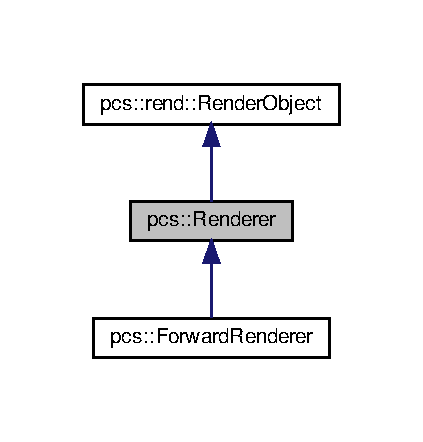
\includegraphics[width=203pt]{classpcs_1_1Renderer__inherit__graph}
\end{center}
\end{figure}


Collaboration diagram for pcs\+:\+:Renderer\+:\nopagebreak
\begin{figure}[H]
\begin{center}
\leavevmode
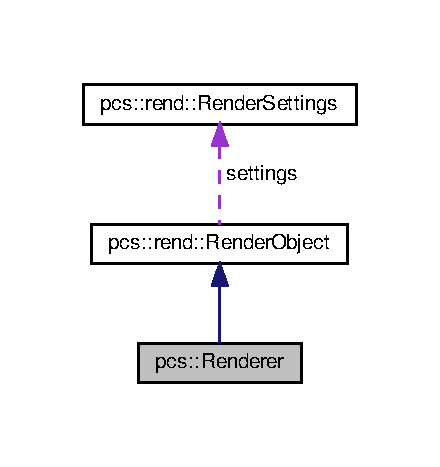
\includegraphics[width=211pt]{classpcs_1_1Renderer__coll__graph}
\end{center}
\end{figure}
\subsection*{Public Member Functions}
\begin{DoxyCompactItemize}
\item 
virtual int \hyperlink{classpcs_1_1Renderer_aba6bdcf38357cdfea898e0f7b3cb1757}{render} (\hyperlink{classpcs_1_1RawModel}{Raw\+Model} $\ast$raw\+Model, \hyperlink{classpcs_1_1ShaderProgram}{Shader\+Program} $\ast$shader, \hyperlink{classpcs_1_1Camera}{Camera} $\ast$camera, unsigned int count=1) const =0
\item 
int \hyperlink{classpcs_1_1Renderer_a4d722540c7af2dfee44726d18aa0ce05}{render} (std\+::vector$<$ \hyperlink{classpcs_1_1Model}{Model} $\ast$$>$ models, \hyperlink{classpcs_1_1ShaderProgram}{Shader\+Program} $\ast$shader, \hyperlink{classpcs_1_1Camera}{Camera} $\ast$camera) const
\end{DoxyCompactItemize}
\subsection*{Static Public Member Functions}
\begin{DoxyCompactItemize}
\item 
static double \& \hyperlink{classpcs_1_1Renderer_a1b1eba1dbd9d5fa3293bfe2295b0ad9d}{get\+Process\+Time} ()
\item 
static unsigned int \& \hyperlink{classpcs_1_1Renderer_a928518fe0b60785048b1a7780df14303}{get\+Thread\+Count} ()
\end{DoxyCompactItemize}
\subsection*{Protected Member Functions}
\begin{DoxyCompactItemize}
\item 
double \hyperlink{classpcs_1_1Renderer_adae0f95f56f7261ec52ea32eaa3ad27b}{process\+Models} (\hyperlink{classpcs_1_1RawModel}{Raw\+Model} $\ast$raw\+Model, std\+::vector$<$ \hyperlink{classpcs_1_1Model}{Model} $\ast$$>$ \&models) const
\end{DoxyCompactItemize}
\subsection*{Additional Inherited Members}


\subsection{Member Function Documentation}
\mbox{\Hypertarget{classpcs_1_1Renderer_a1b1eba1dbd9d5fa3293bfe2295b0ad9d}\label{classpcs_1_1Renderer_a1b1eba1dbd9d5fa3293bfe2295b0ad9d}} 
\index{pcs\+::\+Renderer@{pcs\+::\+Renderer}!get\+Process\+Time@{get\+Process\+Time}}
\index{get\+Process\+Time@{get\+Process\+Time}!pcs\+::\+Renderer@{pcs\+::\+Renderer}}
\subsubsection{\texorpdfstring{get\+Process\+Time()}{getProcessTime()}}
{\footnotesize\ttfamily static double\& pcs\+::\+Renderer\+::get\+Process\+Time (\begin{DoxyParamCaption}{ }\end{DoxyParamCaption})\hspace{0.3cm}{\ttfamily [inline]}, {\ttfamily [static]}}

\mbox{\Hypertarget{classpcs_1_1Renderer_a928518fe0b60785048b1a7780df14303}\label{classpcs_1_1Renderer_a928518fe0b60785048b1a7780df14303}} 
\index{pcs\+::\+Renderer@{pcs\+::\+Renderer}!get\+Thread\+Count@{get\+Thread\+Count}}
\index{get\+Thread\+Count@{get\+Thread\+Count}!pcs\+::\+Renderer@{pcs\+::\+Renderer}}
\subsubsection{\texorpdfstring{get\+Thread\+Count()}{getThreadCount()}}
{\footnotesize\ttfamily static unsigned int\& pcs\+::\+Renderer\+::get\+Thread\+Count (\begin{DoxyParamCaption}{ }\end{DoxyParamCaption})\hspace{0.3cm}{\ttfamily [inline]}, {\ttfamily [static]}}

\mbox{\Hypertarget{classpcs_1_1Renderer_adae0f95f56f7261ec52ea32eaa3ad27b}\label{classpcs_1_1Renderer_adae0f95f56f7261ec52ea32eaa3ad27b}} 
\index{pcs\+::\+Renderer@{pcs\+::\+Renderer}!process\+Models@{process\+Models}}
\index{process\+Models@{process\+Models}!pcs\+::\+Renderer@{pcs\+::\+Renderer}}
\subsubsection{\texorpdfstring{process\+Models()}{processModels()}}
{\footnotesize\ttfamily double pcs\+::\+Renderer\+::process\+Models (\begin{DoxyParamCaption}\item[{\hyperlink{classpcs_1_1RawModel}{Raw\+Model} $\ast$}]{raw\+Model,  }\item[{std\+::vector$<$ \hyperlink{classpcs_1_1Model}{Model} $\ast$$>$ \&}]{models }\end{DoxyParamCaption}) const\hspace{0.3cm}{\ttfamily [protected]}}

\mbox{\Hypertarget{classpcs_1_1Renderer_aba6bdcf38357cdfea898e0f7b3cb1757}\label{classpcs_1_1Renderer_aba6bdcf38357cdfea898e0f7b3cb1757}} 
\index{pcs\+::\+Renderer@{pcs\+::\+Renderer}!render@{render}}
\index{render@{render}!pcs\+::\+Renderer@{pcs\+::\+Renderer}}
\subsubsection{\texorpdfstring{render()}{render()}\hspace{0.1cm}{\footnotesize\ttfamily [1/2]}}
{\footnotesize\ttfamily virtual int pcs\+::\+Renderer\+::render (\begin{DoxyParamCaption}\item[{\hyperlink{classpcs_1_1RawModel}{Raw\+Model} $\ast$}]{raw\+Model,  }\item[{\hyperlink{classpcs_1_1ShaderProgram}{Shader\+Program} $\ast$}]{shader,  }\item[{\hyperlink{classpcs_1_1Camera}{Camera} $\ast$}]{camera,  }\item[{unsigned int}]{count = {\ttfamily 1} }\end{DoxyParamCaption}) const\hspace{0.3cm}{\ttfamily [pure virtual]}}



Implemented in \hyperlink{classpcs_1_1ForwardRenderer_a75527d1b400625fc9b33cddaff76bb33}{pcs\+::\+Forward\+Renderer}.

\mbox{\Hypertarget{classpcs_1_1Renderer_a4d722540c7af2dfee44726d18aa0ce05}\label{classpcs_1_1Renderer_a4d722540c7af2dfee44726d18aa0ce05}} 
\index{pcs\+::\+Renderer@{pcs\+::\+Renderer}!render@{render}}
\index{render@{render}!pcs\+::\+Renderer@{pcs\+::\+Renderer}}
\subsubsection{\texorpdfstring{render()}{render()}\hspace{0.1cm}{\footnotesize\ttfamily [2/2]}}
{\footnotesize\ttfamily int pcs\+::\+Renderer\+::render (\begin{DoxyParamCaption}\item[{std\+::vector$<$ \hyperlink{classpcs_1_1Model}{Model} $\ast$$>$}]{models,  }\item[{\hyperlink{classpcs_1_1ShaderProgram}{Shader\+Program} $\ast$}]{shader,  }\item[{\hyperlink{classpcs_1_1Camera}{Camera} $\ast$}]{camera }\end{DoxyParamCaption}) const}



The documentation for this class was generated from the following files\+:\begin{DoxyCompactItemize}
\item 
include/\+Perceus/\+Core/\+Graphics/\+Rendering/\hyperlink{Renderer_8h}{Renderer.\+h}\item 
src/\+Core/\+Graphics/\+Rendering/\hyperlink{Renderer_8cpp}{Renderer.\+cpp}\end{DoxyCompactItemize}

\hypertarget{classpcs_1_1rend_1_1RenderObject}{}\section{pcs\+:\+:rend\+:\+:Render\+Object Class Reference}
\label{classpcs_1_1rend_1_1RenderObject}\index{pcs\+::rend\+::\+Render\+Object@{pcs\+::rend\+::\+Render\+Object}}


Class for retreiving the currently selected render A\+PI.  




{\ttfamily \#include $<$Render\+Object.\+h$>$}



Inheritance diagram for pcs\+:\+:rend\+:\+:Render\+Object\+:
\nopagebreak
\begin{figure}[H]
\begin{center}
\leavevmode
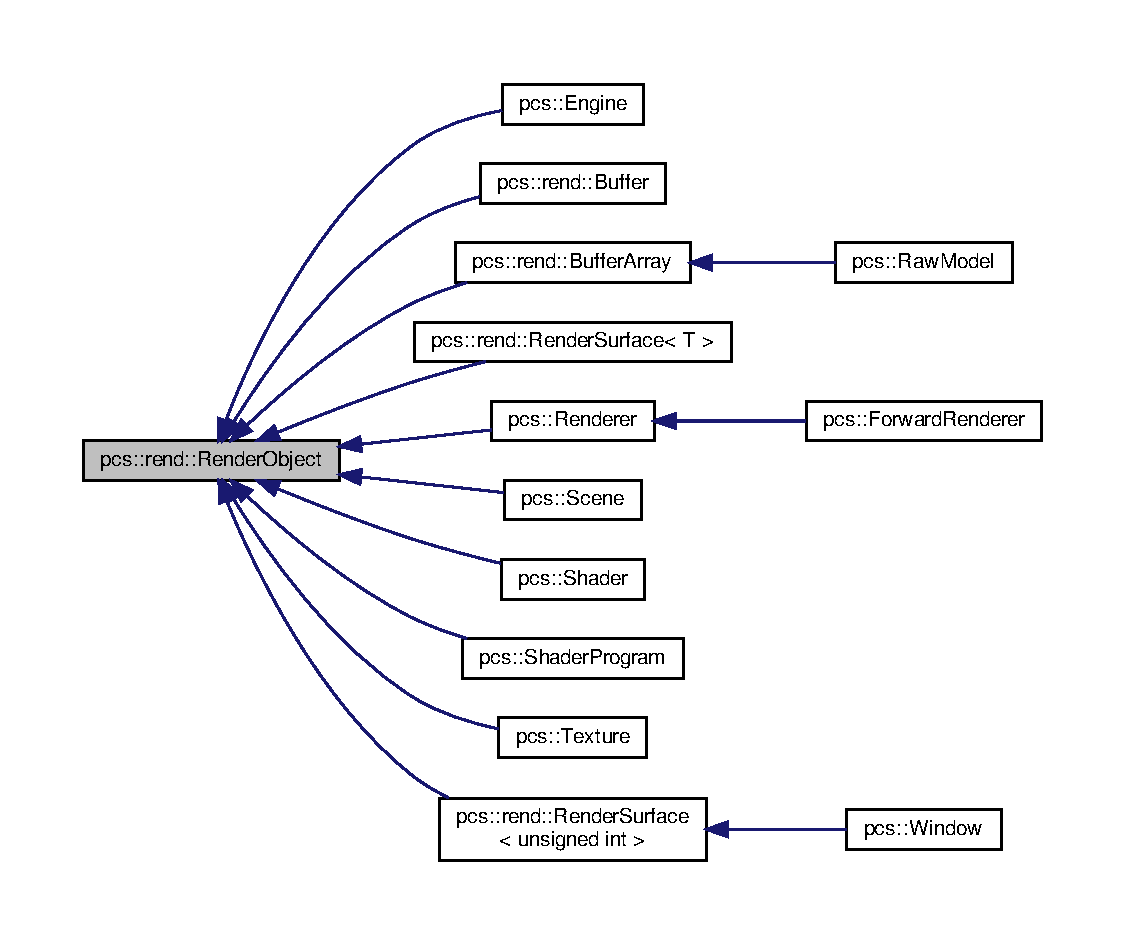
\includegraphics[width=350pt]{classpcs_1_1rend_1_1RenderObject__inherit__graph}
\end{center}
\end{figure}


Collaboration diagram for pcs\+:\+:rend\+:\+:Render\+Object\+:\nopagebreak
\begin{figure}[H]
\begin{center}
\leavevmode
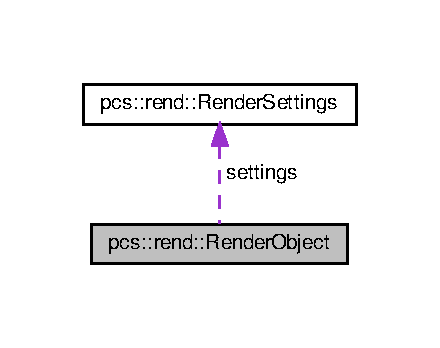
\includegraphics[width=211pt]{classpcs_1_1rend_1_1RenderObject__coll__graph}
\end{center}
\end{figure}
\subsection*{Static Protected Member Functions}
\begin{DoxyCompactItemize}
\item 
static \hyperlink{structpcs_1_1rend_1_1RenderAPI}{Render\+A\+PI} $\ast$ \hyperlink{classpcs_1_1rend_1_1RenderObject_aed66ebea09229bc1b6b1e853813322df}{rend\+A\+PI} ()
\begin{DoxyCompactList}\small\item\em Holds and retreives the currently selected render A\+PI interface. \end{DoxyCompactList}\end{DoxyCompactItemize}
\subsection*{Static Protected Attributes}
\begin{DoxyCompactItemize}
\item 
static \hyperlink{structpcs_1_1rend_1_1RenderSettings}{Render\+Settings} \hyperlink{classpcs_1_1rend_1_1RenderObject_a354e6b71a0f1a7229a5a57944f047ceb}{settings}
\begin{DoxyCompactList}\small\item\em Used for keeping track of the currently selected render A\+PI. \end{DoxyCompactList}\end{DoxyCompactItemize}


\subsection{Detailed Description}
Class for retreiving the currently selected render A\+PI. 

\subsection{Member Function Documentation}
\mbox{\Hypertarget{classpcs_1_1rend_1_1RenderObject_aed66ebea09229bc1b6b1e853813322df}\label{classpcs_1_1rend_1_1RenderObject_aed66ebea09229bc1b6b1e853813322df}} 
\index{pcs\+::rend\+::\+Render\+Object@{pcs\+::rend\+::\+Render\+Object}!rend\+A\+PI@{rend\+A\+PI}}
\index{rend\+A\+PI@{rend\+A\+PI}!pcs\+::rend\+::\+Render\+Object@{pcs\+::rend\+::\+Render\+Object}}
\subsubsection{\texorpdfstring{rend\+A\+P\+I()}{rendAPI()}}
{\footnotesize\ttfamily \hyperlink{structpcs_1_1rend_1_1RenderAPI}{Render\+A\+PI} $\ast$ pcs\+::rend\+::\+Render\+Object\+::rend\+A\+PI (\begin{DoxyParamCaption}{ }\end{DoxyParamCaption})\hspace{0.3cm}{\ttfamily [static]}, {\ttfamily [protected]}}



Holds and retreives the currently selected render A\+PI interface. 

\begin{DoxyReturn}{Returns}
Render\+A\+P\+I$\ast$ Currently selected render A\+PI interface. 
\end{DoxyReturn}


\subsection{Member Data Documentation}
\mbox{\Hypertarget{classpcs_1_1rend_1_1RenderObject_a354e6b71a0f1a7229a5a57944f047ceb}\label{classpcs_1_1rend_1_1RenderObject_a354e6b71a0f1a7229a5a57944f047ceb}} 
\index{pcs\+::rend\+::\+Render\+Object@{pcs\+::rend\+::\+Render\+Object}!settings@{settings}}
\index{settings@{settings}!pcs\+::rend\+::\+Render\+Object@{pcs\+::rend\+::\+Render\+Object}}
\subsubsection{\texorpdfstring{settings}{settings}}
{\footnotesize\ttfamily \hyperlink{structpcs_1_1rend_1_1RenderSettings}{Render\+Settings} pcs\+::rend\+::\+Render\+Object\+::settings\hspace{0.3cm}{\ttfamily [static]}, {\ttfamily [protected]}}



Used for keeping track of the currently selected render A\+PI. 



The documentation for this class was generated from the following files\+:\begin{DoxyCompactItemize}
\item 
include/\+Perceus/\+Core/\+Graphics/\+Rendering/\hyperlink{RenderObject_8h}{Render\+Object.\+h}\item 
src/\+Core/\+Graphics/\+Rendering/\hyperlink{RenderObject_8cpp}{Render\+Object.\+cpp}\end{DoxyCompactItemize}

\hypertarget{structpcs_1_1rend_1_1RenderSettings}{}\section{pcs\+:\+:rend\+:\+:Render\+Settings Struct Reference}
\label{structpcs_1_1rend_1_1RenderSettings}\index{pcs\+::rend\+::\+Render\+Settings@{pcs\+::rend\+::\+Render\+Settings}}


Container for choosing various A\+PI types.  




{\ttfamily \#include $<$Render\+Object.\+h$>$}

\subsection*{Public Member Functions}
\begin{DoxyCompactItemize}
\item 
const char $\ast$ \hyperlink{structpcs_1_1rend_1_1RenderSettings_acb1a74d9eb282c46471576a5ddaa8c31}{get\+A\+P\+I\+Name} (\hyperlink{namespacepcs_1_1rend_a9627be55d9b373e41fd62c11e118e68f}{Render\+A\+P\+I\+Type} type) const
\end{DoxyCompactItemize}
\subsection*{Public Attributes}
\begin{DoxyCompactItemize}
\item 
\hyperlink{namespacepcs_1_1rend_a9627be55d9b373e41fd62c11e118e68f}{Render\+A\+P\+I\+Type} \hyperlink{structpcs_1_1rend_1_1RenderSettings_a62f0625f562fa1c6a4f7be8c783931f5}{api} = \hyperlink{namespacepcs_1_1rend_a9627be55d9b373e41fd62c11e118e68fab356921baf7069b879f7bab06b3ae51e}{Open\+GL}
\end{DoxyCompactItemize}


\subsection{Detailed Description}
Container for choosing various A\+PI types. 

\subsection{Member Function Documentation}
\mbox{\Hypertarget{structpcs_1_1rend_1_1RenderSettings_acb1a74d9eb282c46471576a5ddaa8c31}\label{structpcs_1_1rend_1_1RenderSettings_acb1a74d9eb282c46471576a5ddaa8c31}} 
\index{pcs\+::rend\+::\+Render\+Settings@{pcs\+::rend\+::\+Render\+Settings}!get\+A\+P\+I\+Name@{get\+A\+P\+I\+Name}}
\index{get\+A\+P\+I\+Name@{get\+A\+P\+I\+Name}!pcs\+::rend\+::\+Render\+Settings@{pcs\+::rend\+::\+Render\+Settings}}
\subsubsection{\texorpdfstring{get\+A\+P\+I\+Name()}{getAPIName()}}
{\footnotesize\ttfamily const char$\ast$ pcs\+::rend\+::\+Render\+Settings\+::get\+A\+P\+I\+Name (\begin{DoxyParamCaption}\item[{\hyperlink{namespacepcs_1_1rend_a9627be55d9b373e41fd62c11e118e68f}{Render\+A\+P\+I\+Type}}]{type }\end{DoxyParamCaption}) const\hspace{0.3cm}{\ttfamily [inline]}}



\subsection{Member Data Documentation}
\mbox{\Hypertarget{structpcs_1_1rend_1_1RenderSettings_a62f0625f562fa1c6a4f7be8c783931f5}\label{structpcs_1_1rend_1_1RenderSettings_a62f0625f562fa1c6a4f7be8c783931f5}} 
\index{pcs\+::rend\+::\+Render\+Settings@{pcs\+::rend\+::\+Render\+Settings}!api@{api}}
\index{api@{api}!pcs\+::rend\+::\+Render\+Settings@{pcs\+::rend\+::\+Render\+Settings}}
\subsubsection{\texorpdfstring{api}{api}}
{\footnotesize\ttfamily \hyperlink{namespacepcs_1_1rend_a9627be55d9b373e41fd62c11e118e68f}{Render\+A\+P\+I\+Type} pcs\+::rend\+::\+Render\+Settings\+::api = \hyperlink{namespacepcs_1_1rend_a9627be55d9b373e41fd62c11e118e68fab356921baf7069b879f7bab06b3ae51e}{Open\+GL}}



The documentation for this struct was generated from the following file\+:\begin{DoxyCompactItemize}
\item 
include/\+Perceus/\+Core/\+Graphics/\+Rendering/\hyperlink{RenderObject_8h}{Render\+Object.\+h}\end{DoxyCompactItemize}

\hypertarget{classpcs_1_1rend_1_1RenderSurface}{}\section{pcs\+:\+:rend\+:\+:Render\+Surface$<$ T $>$ Class Template Reference}
\label{classpcs_1_1rend_1_1RenderSurface}\index{pcs\+::rend\+::\+Render\+Surface$<$ T $>$@{pcs\+::rend\+::\+Render\+Surface$<$ T $>$}}


Class that handles basic rendering functionality.  




{\ttfamily \#include $<$Render\+Surface.\+h$>$}



Inheritance diagram for pcs\+:\+:rend\+:\+:Render\+Surface$<$ T $>$\+:\nopagebreak
\begin{figure}[H]
\begin{center}
\leavevmode
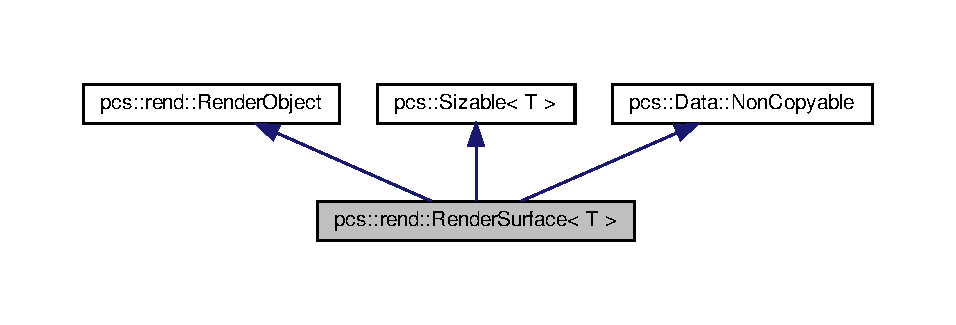
\includegraphics[width=350pt]{classpcs_1_1rend_1_1RenderSurface__inherit__graph}
\end{center}
\end{figure}


Collaboration diagram for pcs\+:\+:rend\+:\+:Render\+Surface$<$ T $>$\+:\nopagebreak
\begin{figure}[H]
\begin{center}
\leavevmode
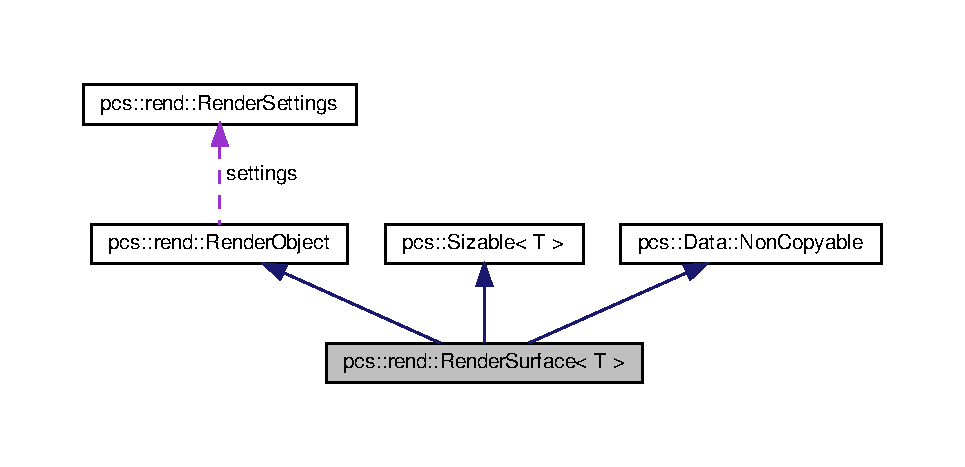
\includegraphics[width=350pt]{classpcs_1_1rend_1_1RenderSurface__coll__graph}
\end{center}
\end{figure}
\subsection*{Public Member Functions}
\begin{DoxyCompactItemize}
\item 
\hyperlink{classpcs_1_1rend_1_1RenderSurface_a908ee596a69b977a74270f03ecc90808}{Render\+Surface} (const T width, const T height)
\item 
void \hyperlink{classpcs_1_1rend_1_1RenderSurface_ac875e478b7cbf438aa541f31fba6b750}{clear} (\hyperlink{structpcs_1_1Color}{Color} color=\hyperlink{structpcs_1_1Color}{Color}(0, 0, 0)) const
\item 
virtual void \hyperlink{classpcs_1_1rend_1_1RenderSurface_a79c0b291ed5a7b901fe4233bf8b376f2}{bind} ()=0
\item 
virtual void \hyperlink{classpcs_1_1rend_1_1RenderSurface_aacb7218feb1973ee4b0486494fcd8c88}{unbind} () const =0
\item 
void $\ast$$\ast$ \hyperlink{classpcs_1_1rend_1_1RenderSurface_a54cbf8c34638a82bfe02bc1f1663a4ab}{get\+A\+P\+I\+Loc} ()
\begin{DoxyCompactList}\small\item\em Returns the api pointer. \end{DoxyCompactList}\end{DoxyCompactItemize}
\subsection*{Protected Attributes}
\begin{DoxyCompactItemize}
\item 
void $\ast$ \hyperlink{classpcs_1_1rend_1_1RenderSurface_ac991c5aaed973108fa4bb97d605f02cc}{api\+P\+TR} = nullptr
\begin{DoxyCompactList}\small\item\em Type-\/independant pointer to an object needed by the render api. \end{DoxyCompactList}\end{DoxyCompactItemize}
\subsection*{Additional Inherited Members}


\subsection{Detailed Description}
\subsubsection*{template$<$typename T$>$\newline
class pcs\+::rend\+::\+Render\+Surface$<$ T $>$}

Class that handles basic rendering functionality. 


\begin{DoxyTemplParams}{Template Parameters}
{\em T} & Type which \hyperlink{structpcs_1_1Sizable}{Sizable} is to be \\
\hline
\end{DoxyTemplParams}


\subsection{Constructor \& Destructor Documentation}
\mbox{\Hypertarget{classpcs_1_1rend_1_1RenderSurface_a908ee596a69b977a74270f03ecc90808}\label{classpcs_1_1rend_1_1RenderSurface_a908ee596a69b977a74270f03ecc90808}} 
\index{pcs\+::rend\+::\+Render\+Surface@{pcs\+::rend\+::\+Render\+Surface}!Render\+Surface@{Render\+Surface}}
\index{Render\+Surface@{Render\+Surface}!pcs\+::rend\+::\+Render\+Surface@{pcs\+::rend\+::\+Render\+Surface}}
\subsubsection{\texorpdfstring{Render\+Surface()}{RenderSurface()}}
{\footnotesize\ttfamily template$<$typename T$>$ \\
\hyperlink{classpcs_1_1rend_1_1RenderSurface}{pcs\+::rend\+::\+Render\+Surface}$<$ T $>$\+::\hyperlink{classpcs_1_1rend_1_1RenderSurface}{Render\+Surface} (\begin{DoxyParamCaption}\item[{const T}]{width,  }\item[{const T}]{height }\end{DoxyParamCaption})\hspace{0.3cm}{\ttfamily [inline]}}



\subsection{Member Function Documentation}
\mbox{\Hypertarget{classpcs_1_1rend_1_1RenderSurface_a79c0b291ed5a7b901fe4233bf8b376f2}\label{classpcs_1_1rend_1_1RenderSurface_a79c0b291ed5a7b901fe4233bf8b376f2}} 
\index{pcs\+::rend\+::\+Render\+Surface@{pcs\+::rend\+::\+Render\+Surface}!bind@{bind}}
\index{bind@{bind}!pcs\+::rend\+::\+Render\+Surface@{pcs\+::rend\+::\+Render\+Surface}}
\subsubsection{\texorpdfstring{bind()}{bind()}}
{\footnotesize\ttfamily template$<$typename T$>$ \\
virtual void \hyperlink{classpcs_1_1rend_1_1RenderSurface}{pcs\+::rend\+::\+Render\+Surface}$<$ T $>$\+::bind (\begin{DoxyParamCaption}{ }\end{DoxyParamCaption})\hspace{0.3cm}{\ttfamily [pure virtual]}}



Implemented in \hyperlink{classpcs_1_1Window_aa6e00bee6910b3146481dee7aab69cfb}{pcs\+::\+Window}.

\mbox{\Hypertarget{classpcs_1_1rend_1_1RenderSurface_ac875e478b7cbf438aa541f31fba6b750}\label{classpcs_1_1rend_1_1RenderSurface_ac875e478b7cbf438aa541f31fba6b750}} 
\index{pcs\+::rend\+::\+Render\+Surface@{pcs\+::rend\+::\+Render\+Surface}!clear@{clear}}
\index{clear@{clear}!pcs\+::rend\+::\+Render\+Surface@{pcs\+::rend\+::\+Render\+Surface}}
\subsubsection{\texorpdfstring{clear()}{clear()}}
{\footnotesize\ttfamily template$<$typename T$>$ \\
void \hyperlink{classpcs_1_1rend_1_1RenderSurface}{pcs\+::rend\+::\+Render\+Surface}$<$ T $>$\+::clear (\begin{DoxyParamCaption}\item[{\hyperlink{structpcs_1_1Color}{Color}}]{color = {\ttfamily \hyperlink{structpcs_1_1Color}{Color}(0,~0,~0)} }\end{DoxyParamCaption}) const\hspace{0.3cm}{\ttfamily [inline]}}

\mbox{\Hypertarget{classpcs_1_1rend_1_1RenderSurface_a54cbf8c34638a82bfe02bc1f1663a4ab}\label{classpcs_1_1rend_1_1RenderSurface_a54cbf8c34638a82bfe02bc1f1663a4ab}} 
\index{pcs\+::rend\+::\+Render\+Surface@{pcs\+::rend\+::\+Render\+Surface}!get\+A\+P\+I\+Loc@{get\+A\+P\+I\+Loc}}
\index{get\+A\+P\+I\+Loc@{get\+A\+P\+I\+Loc}!pcs\+::rend\+::\+Render\+Surface@{pcs\+::rend\+::\+Render\+Surface}}
\subsubsection{\texorpdfstring{get\+A\+P\+I\+Loc()}{getAPILoc()}}
{\footnotesize\ttfamily template$<$typename T$>$ \\
void$\ast$$\ast$ \hyperlink{classpcs_1_1rend_1_1RenderSurface}{pcs\+::rend\+::\+Render\+Surface}$<$ T $>$\+::get\+A\+P\+I\+Loc (\begin{DoxyParamCaption}{ }\end{DoxyParamCaption})\hspace{0.3cm}{\ttfamily [inline]}}



Returns the api pointer. 

\mbox{\Hypertarget{classpcs_1_1rend_1_1RenderSurface_aacb7218feb1973ee4b0486494fcd8c88}\label{classpcs_1_1rend_1_1RenderSurface_aacb7218feb1973ee4b0486494fcd8c88}} 
\index{pcs\+::rend\+::\+Render\+Surface@{pcs\+::rend\+::\+Render\+Surface}!unbind@{unbind}}
\index{unbind@{unbind}!pcs\+::rend\+::\+Render\+Surface@{pcs\+::rend\+::\+Render\+Surface}}
\subsubsection{\texorpdfstring{unbind()}{unbind()}}
{\footnotesize\ttfamily template$<$typename T$>$ \\
virtual void \hyperlink{classpcs_1_1rend_1_1RenderSurface}{pcs\+::rend\+::\+Render\+Surface}$<$ T $>$\+::unbind (\begin{DoxyParamCaption}{ }\end{DoxyParamCaption}) const\hspace{0.3cm}{\ttfamily [pure virtual]}}



Implemented in \hyperlink{classpcs_1_1Window_a4d103be3712fbb051d7c4d446a266de0}{pcs\+::\+Window}.



\subsection{Member Data Documentation}
\mbox{\Hypertarget{classpcs_1_1rend_1_1RenderSurface_ac991c5aaed973108fa4bb97d605f02cc}\label{classpcs_1_1rend_1_1RenderSurface_ac991c5aaed973108fa4bb97d605f02cc}} 
\index{pcs\+::rend\+::\+Render\+Surface@{pcs\+::rend\+::\+Render\+Surface}!api\+P\+TR@{api\+P\+TR}}
\index{api\+P\+TR@{api\+P\+TR}!pcs\+::rend\+::\+Render\+Surface@{pcs\+::rend\+::\+Render\+Surface}}
\subsubsection{\texorpdfstring{api\+P\+TR}{apiPTR}}
{\footnotesize\ttfamily template$<$typename T$>$ \\
void$\ast$ \hyperlink{classpcs_1_1rend_1_1RenderSurface}{pcs\+::rend\+::\+Render\+Surface}$<$ T $>$\+::api\+P\+TR = nullptr\hspace{0.3cm}{\ttfamily [protected]}}



Type-\/independant pointer to an object needed by the render api. 



The documentation for this class was generated from the following file\+:\begin{DoxyCompactItemize}
\item 
include/\+Perceus/\+Core/\+Graphics/\+Rendering/\hyperlink{RenderSurface_8h}{Render\+Surface.\+h}\end{DoxyCompactItemize}

\hypertarget{classpcs_1_1Scene}{}\section{pcs\+:\+:Scene Class Reference}
\label{classpcs_1_1Scene}\index{pcs\+::\+Scene@{pcs\+::\+Scene}}


{\ttfamily \#include $<$Scene.\+h$>$}



Inheritance diagram for pcs\+:\+:Scene\+:\nopagebreak
\begin{figure}[H]
\begin{center}
\leavevmode
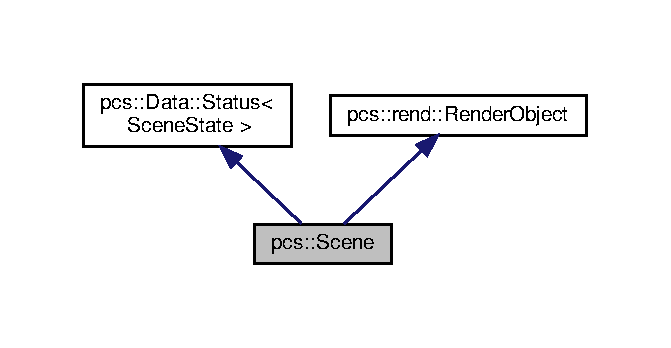
\includegraphics[width=322pt]{classpcs_1_1Scene__inherit__graph}
\end{center}
\end{figure}


Collaboration diagram for pcs\+:\+:Scene\+:\nopagebreak
\begin{figure}[H]
\begin{center}
\leavevmode
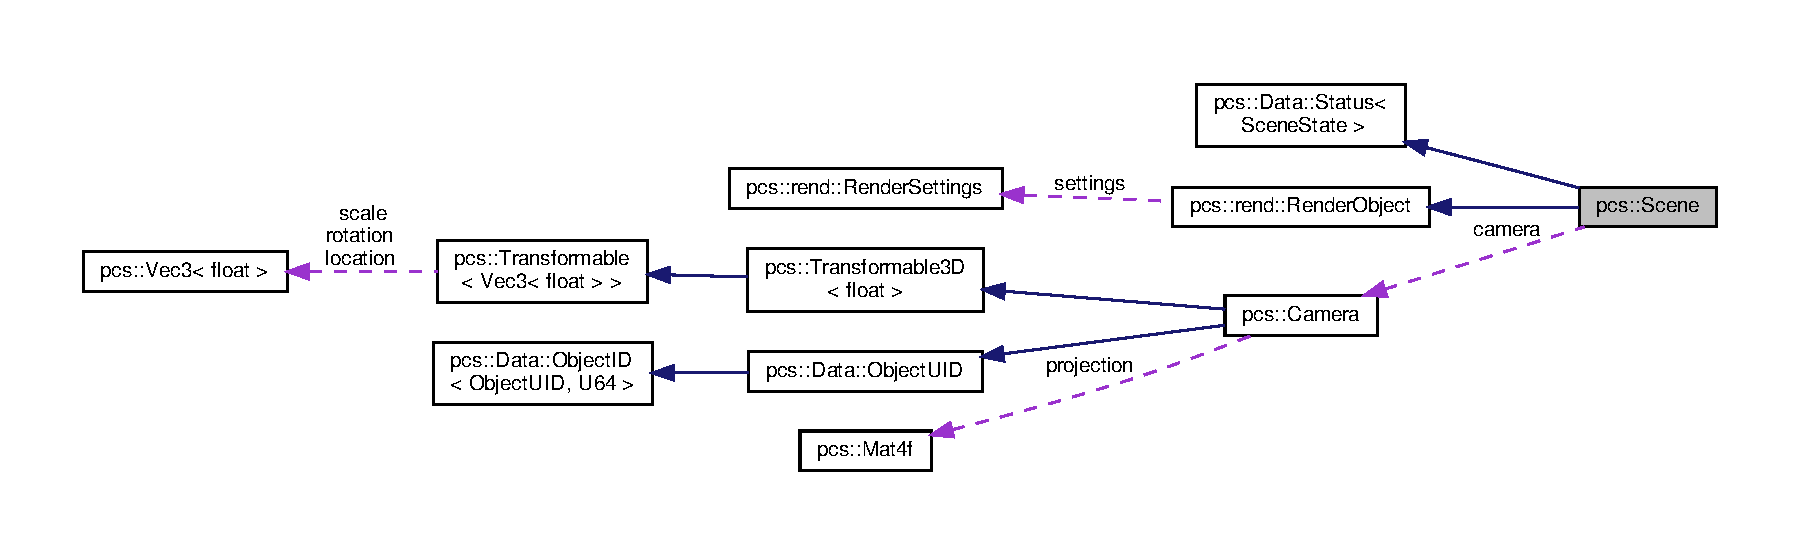
\includegraphics[width=350pt]{classpcs_1_1Scene__coll__graph}
\end{center}
\end{figure}
\subsection*{Public Member Functions}
\begin{DoxyCompactItemize}
\item 
\hyperlink{classpcs_1_1Scene_a04a77b0c67dc42c11d5c50a07ab3a06f}{Scene} (float F\+OV=90.f)
\item 
virtual \hyperlink{classpcs_1_1Scene_a106aca266becd518d47821e08a87cf6f}{$\sim$\+Scene} ()
\item 
\hyperlink{classpcs_1_1Camera}{Camera} \& \hyperlink{classpcs_1_1Scene_a94be9eaa37239c5c0a854af148cf0225}{get\+Camera} ()
\end{DoxyCompactItemize}
\subsection*{Protected Member Functions}
\begin{DoxyCompactItemize}
\item 
bool \hyperlink{classpcs_1_1Scene_ab6c463fedfc6499998d55206aa9afeb9}{poll\+Event} (\hyperlink{classpcs_1_1Event}{Event} $\ast$$\ast$event)
\item 
virtual void \hyperlink{classpcs_1_1Scene_ad1ed5ae1d53a533e2970de85093a4bc4}{render} ()=0
\end{DoxyCompactItemize}
\subsection*{Private Member Functions}
\begin{DoxyCompactItemize}
\item 
void \hyperlink{classpcs_1_1Scene_ad5f0807caa705da2b3782ad4cf2619a8}{\+\_\+render} ()
\end{DoxyCompactItemize}
\subsection*{Private Attributes}
\begin{DoxyCompactItemize}
\item 
\hyperlink{classpcs_1_1Camera}{Camera} \hyperlink{classpcs_1_1Scene_ad71d97a418c46759bda1c84742ab9fd3}{camera}
\end{DoxyCompactItemize}
\subsection*{Friends}
\begin{DoxyCompactItemize}
\item 
class \hyperlink{classpcs_1_1Scene_a3e1914489e4bed4f9f23cdeab34a43dc}{Engine}
\end{DoxyCompactItemize}
\subsection*{Additional Inherited Members}


\subsection{Constructor \& Destructor Documentation}
\mbox{\Hypertarget{classpcs_1_1Scene_a04a77b0c67dc42c11d5c50a07ab3a06f}\label{classpcs_1_1Scene_a04a77b0c67dc42c11d5c50a07ab3a06f}} 
\index{pcs\+::\+Scene@{pcs\+::\+Scene}!Scene@{Scene}}
\index{Scene@{Scene}!pcs\+::\+Scene@{pcs\+::\+Scene}}
\subsubsection{\texorpdfstring{Scene()}{Scene()}}
{\footnotesize\ttfamily pcs\+::\+Scene\+::\+Scene (\begin{DoxyParamCaption}\item[{float}]{F\+OV = {\ttfamily 90.f} }\end{DoxyParamCaption})}

\mbox{\Hypertarget{classpcs_1_1Scene_a106aca266becd518d47821e08a87cf6f}\label{classpcs_1_1Scene_a106aca266becd518d47821e08a87cf6f}} 
\index{pcs\+::\+Scene@{pcs\+::\+Scene}!````~Scene@{$\sim$\+Scene}}
\index{````~Scene@{$\sim$\+Scene}!pcs\+::\+Scene@{pcs\+::\+Scene}}
\subsubsection{\texorpdfstring{$\sim$\+Scene()}{~Scene()}}
{\footnotesize\ttfamily pcs\+::\+Scene\+::$\sim$\+Scene (\begin{DoxyParamCaption}{ }\end{DoxyParamCaption})\hspace{0.3cm}{\ttfamily [virtual]}}



\subsection{Member Function Documentation}
\mbox{\Hypertarget{classpcs_1_1Scene_ad5f0807caa705da2b3782ad4cf2619a8}\label{classpcs_1_1Scene_ad5f0807caa705da2b3782ad4cf2619a8}} 
\index{pcs\+::\+Scene@{pcs\+::\+Scene}!\+\_\+render@{\+\_\+render}}
\index{\+\_\+render@{\+\_\+render}!pcs\+::\+Scene@{pcs\+::\+Scene}}
\subsubsection{\texorpdfstring{\+\_\+render()}{\_render()}}
{\footnotesize\ttfamily void pcs\+::\+Scene\+::\+\_\+render (\begin{DoxyParamCaption}{ }\end{DoxyParamCaption})\hspace{0.3cm}{\ttfamily [private]}}

\mbox{\Hypertarget{classpcs_1_1Scene_a94be9eaa37239c5c0a854af148cf0225}\label{classpcs_1_1Scene_a94be9eaa37239c5c0a854af148cf0225}} 
\index{pcs\+::\+Scene@{pcs\+::\+Scene}!get\+Camera@{get\+Camera}}
\index{get\+Camera@{get\+Camera}!pcs\+::\+Scene@{pcs\+::\+Scene}}
\subsubsection{\texorpdfstring{get\+Camera()}{getCamera()}}
{\footnotesize\ttfamily \hyperlink{classpcs_1_1Camera}{Camera}\& pcs\+::\+Scene\+::get\+Camera (\begin{DoxyParamCaption}{ }\end{DoxyParamCaption})\hspace{0.3cm}{\ttfamily [inline]}}

\mbox{\Hypertarget{classpcs_1_1Scene_ab6c463fedfc6499998d55206aa9afeb9}\label{classpcs_1_1Scene_ab6c463fedfc6499998d55206aa9afeb9}} 
\index{pcs\+::\+Scene@{pcs\+::\+Scene}!poll\+Event@{poll\+Event}}
\index{poll\+Event@{poll\+Event}!pcs\+::\+Scene@{pcs\+::\+Scene}}
\subsubsection{\texorpdfstring{poll\+Event()}{pollEvent()}}
{\footnotesize\ttfamily bool pcs\+::\+Scene\+::poll\+Event (\begin{DoxyParamCaption}\item[{\hyperlink{classpcs_1_1Event}{Event} $\ast$$\ast$}]{event }\end{DoxyParamCaption})\hspace{0.3cm}{\ttfamily [protected]}}

\mbox{\Hypertarget{classpcs_1_1Scene_ad1ed5ae1d53a533e2970de85093a4bc4}\label{classpcs_1_1Scene_ad1ed5ae1d53a533e2970de85093a4bc4}} 
\index{pcs\+::\+Scene@{pcs\+::\+Scene}!render@{render}}
\index{render@{render}!pcs\+::\+Scene@{pcs\+::\+Scene}}
\subsubsection{\texorpdfstring{render()}{render()}}
{\footnotesize\ttfamily virtual void pcs\+::\+Scene\+::render (\begin{DoxyParamCaption}{ }\end{DoxyParamCaption})\hspace{0.3cm}{\ttfamily [protected]}, {\ttfamily [pure virtual]}}



\subsection{Friends And Related Function Documentation}
\mbox{\Hypertarget{classpcs_1_1Scene_a3e1914489e4bed4f9f23cdeab34a43dc}\label{classpcs_1_1Scene_a3e1914489e4bed4f9f23cdeab34a43dc}} 
\index{pcs\+::\+Scene@{pcs\+::\+Scene}!Engine@{Engine}}
\index{Engine@{Engine}!pcs\+::\+Scene@{pcs\+::\+Scene}}
\subsubsection{\texorpdfstring{Engine}{Engine}}
{\footnotesize\ttfamily friend class \hyperlink{classpcs_1_1Engine}{Engine}\hspace{0.3cm}{\ttfamily [friend]}}



\subsection{Member Data Documentation}
\mbox{\Hypertarget{classpcs_1_1Scene_ad71d97a418c46759bda1c84742ab9fd3}\label{classpcs_1_1Scene_ad71d97a418c46759bda1c84742ab9fd3}} 
\index{pcs\+::\+Scene@{pcs\+::\+Scene}!camera@{camera}}
\index{camera@{camera}!pcs\+::\+Scene@{pcs\+::\+Scene}}
\subsubsection{\texorpdfstring{camera}{camera}}
{\footnotesize\ttfamily \hyperlink{classpcs_1_1Camera}{Camera} pcs\+::\+Scene\+::camera\hspace{0.3cm}{\ttfamily [private]}}



The documentation for this class was generated from the following files\+:\begin{DoxyCompactItemize}
\item 
include/\+Perceus/\+Core/\hyperlink{Scene_8h}{Scene.\+h}\item 
src/\+Core/\hyperlink{Scene_8cpp}{Scene.\+cpp}\end{DoxyCompactItemize}

\hypertarget{classpcs_1_1Shader}{}\section{pcs\+:\+:Shader Class Reference}
\label{classpcs_1_1Shader}\index{pcs\+::\+Shader@{pcs\+::\+Shader}}


{\ttfamily \#include $<$Shader.\+h$>$}



Inheritance diagram for pcs\+:\+:Shader\+:\nopagebreak
\begin{figure}[H]
\begin{center}
\leavevmode
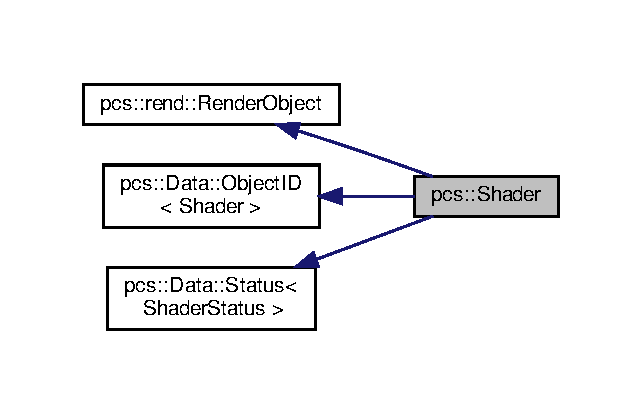
\includegraphics[width=308pt]{classpcs_1_1Shader__inherit__graph}
\end{center}
\end{figure}


Collaboration diagram for pcs\+:\+:Shader\+:\nopagebreak
\begin{figure}[H]
\begin{center}
\leavevmode
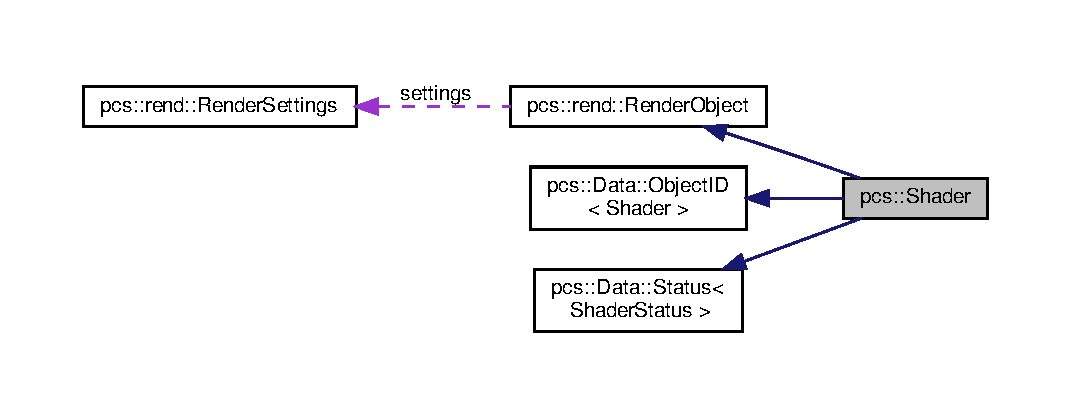
\includegraphics[width=350pt]{classpcs_1_1Shader__coll__graph}
\end{center}
\end{figure}
\subsection*{Public Member Functions}
\begin{DoxyCompactItemize}
\item 
\hyperlink{classpcs_1_1Shader_a011160b22999ecbbdaf03463ec17e2be}{Shader} (\hyperlink{namespacepcs_a2f6dfe5fadf3611302a9b7259502c3c9}{Shader\+Type} t)
\item 
\hyperlink{classpcs_1_1Shader_ae29be85176bf296e0b59da4e88f52ba4}{$\sim$\+Shader} ()
\item 
int \hyperlink{classpcs_1_1Shader_ae672370f28f362074596bb9d410738cd}{load\+Shader\+From\+String} (std\+::string str)
\item 
\hyperlink{namespacepcs_a2f6dfe5fadf3611302a9b7259502c3c9}{Shader\+Type} \hyperlink{classpcs_1_1Shader_ab2846a8669b4fa1904c921fa1d4bf083}{get\+Type} () const
\end{DoxyCompactItemize}
\subsection*{Private Attributes}
\begin{DoxyCompactItemize}
\item 
\hyperlink{namespacepcs_a2f6dfe5fadf3611302a9b7259502c3c9}{Shader\+Type} \hyperlink{classpcs_1_1Shader_a0f8b1769a66ad5d63b4357287ff0f6f8}{type}
\end{DoxyCompactItemize}
\subsection*{Additional Inherited Members}


\subsection{Constructor \& Destructor Documentation}
\mbox{\Hypertarget{classpcs_1_1Shader_a011160b22999ecbbdaf03463ec17e2be}\label{classpcs_1_1Shader_a011160b22999ecbbdaf03463ec17e2be}} 
\index{pcs\+::\+Shader@{pcs\+::\+Shader}!Shader@{Shader}}
\index{Shader@{Shader}!pcs\+::\+Shader@{pcs\+::\+Shader}}
\subsubsection{\texorpdfstring{Shader()}{Shader()}}
{\footnotesize\ttfamily pcs\+::\+Shader\+::\+Shader (\begin{DoxyParamCaption}\item[{\hyperlink{namespacepcs_a2f6dfe5fadf3611302a9b7259502c3c9}{Shader\+Type}}]{t }\end{DoxyParamCaption})}

\mbox{\Hypertarget{classpcs_1_1Shader_ae29be85176bf296e0b59da4e88f52ba4}\label{classpcs_1_1Shader_ae29be85176bf296e0b59da4e88f52ba4}} 
\index{pcs\+::\+Shader@{pcs\+::\+Shader}!````~Shader@{$\sim$\+Shader}}
\index{````~Shader@{$\sim$\+Shader}!pcs\+::\+Shader@{pcs\+::\+Shader}}
\subsubsection{\texorpdfstring{$\sim$\+Shader()}{~Shader()}}
{\footnotesize\ttfamily pcs\+::\+Shader\+::$\sim$\+Shader (\begin{DoxyParamCaption}{ }\end{DoxyParamCaption})}



\subsection{Member Function Documentation}
\mbox{\Hypertarget{classpcs_1_1Shader_ab2846a8669b4fa1904c921fa1d4bf083}\label{classpcs_1_1Shader_ab2846a8669b4fa1904c921fa1d4bf083}} 
\index{pcs\+::\+Shader@{pcs\+::\+Shader}!get\+Type@{get\+Type}}
\index{get\+Type@{get\+Type}!pcs\+::\+Shader@{pcs\+::\+Shader}}
\subsubsection{\texorpdfstring{get\+Type()}{getType()}}
{\footnotesize\ttfamily \hyperlink{namespacepcs_a2f6dfe5fadf3611302a9b7259502c3c9}{Shader\+Type} pcs\+::\+Shader\+::get\+Type (\begin{DoxyParamCaption}{ }\end{DoxyParamCaption}) const\hspace{0.3cm}{\ttfamily [inline]}}

\mbox{\Hypertarget{classpcs_1_1Shader_ae672370f28f362074596bb9d410738cd}\label{classpcs_1_1Shader_ae672370f28f362074596bb9d410738cd}} 
\index{pcs\+::\+Shader@{pcs\+::\+Shader}!load\+Shader\+From\+String@{load\+Shader\+From\+String}}
\index{load\+Shader\+From\+String@{load\+Shader\+From\+String}!pcs\+::\+Shader@{pcs\+::\+Shader}}
\subsubsection{\texorpdfstring{load\+Shader\+From\+String()}{loadShaderFromString()}}
{\footnotesize\ttfamily int pcs\+::\+Shader\+::load\+Shader\+From\+String (\begin{DoxyParamCaption}\item[{std\+::string}]{str }\end{DoxyParamCaption})}



\subsection{Member Data Documentation}
\mbox{\Hypertarget{classpcs_1_1Shader_a0f8b1769a66ad5d63b4357287ff0f6f8}\label{classpcs_1_1Shader_a0f8b1769a66ad5d63b4357287ff0f6f8}} 
\index{pcs\+::\+Shader@{pcs\+::\+Shader}!type@{type}}
\index{type@{type}!pcs\+::\+Shader@{pcs\+::\+Shader}}
\subsubsection{\texorpdfstring{type}{type}}
{\footnotesize\ttfamily \hyperlink{namespacepcs_a2f6dfe5fadf3611302a9b7259502c3c9}{Shader\+Type} pcs\+::\+Shader\+::type\hspace{0.3cm}{\ttfamily [private]}}



The documentation for this class was generated from the following files\+:\begin{DoxyCompactItemize}
\item 
include/\+Perceus/\+Core/\+Graphics/\+Rendering/\+Shaders/\hyperlink{Shader_8h}{Shader.\+h}\item 
src/\+Core/\+Graphics/\+Rendering/\+Shaders/\hyperlink{Shader_8cpp}{Shader.\+cpp}\end{DoxyCompactItemize}

\hypertarget{classpcs_1_1ShaderProgram}{}\section{pcs\+:\+:Shader\+Program Class Reference}
\label{classpcs_1_1ShaderProgram}\index{pcs\+::\+Shader\+Program@{pcs\+::\+Shader\+Program}}


{\ttfamily \#include $<$Shader\+Program.\+h$>$}



Inheritance diagram for pcs\+:\+:Shader\+Program\+:\nopagebreak
\begin{figure}[H]
\begin{center}
\leavevmode
\includegraphics[width=326pt]{classpcs_1_1ShaderProgram__inherit__graph}
\end{center}
\end{figure}


Collaboration diagram for pcs\+:\+:Shader\+Program\+:\nopagebreak
\begin{figure}[H]
\begin{center}
\leavevmode
\includegraphics[width=330pt]{classpcs_1_1ShaderProgram__coll__graph}
\end{center}
\end{figure}
\subsection*{Public Member Functions}
\begin{DoxyCompactItemize}
\item 
\hyperlink{classpcs_1_1ShaderProgram_aaf1133ce281667af24c085c680bd3aa3}{Shader\+Program} ()
\item 
\hyperlink{classpcs_1_1ShaderProgram_a6590bd48ce2dcba47c4a7f384d5d3316}{$\sim$\+Shader\+Program} ()
\item 
\hyperlink{classpcs_1_1Shader}{Shader} \& \hyperlink{classpcs_1_1ShaderProgram_ac1bc6629613f24f64887d224accd3aa8}{get\+Shader} (\hyperlink{namespacepcs_a2f6dfe5fadf3611302a9b7259502c3c9}{Shader\+Type} type)
\item 
bool \hyperlink{classpcs_1_1ShaderProgram_ae362fd3f64327ed7d670fee03d28ab27}{link} ()
\item 
bool \hyperlink{classpcs_1_1ShaderProgram_a59765d6a577e400ef261ec9e9cfa7078}{set\+Uniform} (const char $\ast$name, const \hyperlink{structpcs_1_1Mat4f}{Mat4f} \&matrix)
\item 
bool \hyperlink{classpcs_1_1ShaderProgram_a1ff8e923df23c341d5609ca4e65a2dad}{set\+Uniform} (const char $\ast$name, const \hyperlink{namespacepcs_a68e0f517680976c17c810ffe6952cbab}{Vec3f} \&var)
\item 
bool \hyperlink{classpcs_1_1ShaderProgram_af37a2a9c024a7f6dca60f10ab281510d}{set\+Uniform} (const char $\ast$name, const int \&var)
\item 
void \hyperlink{classpcs_1_1ShaderProgram_a48d59dd2b34d48355ba56dd6a85eb7cf}{use} () const
\item 
void \hyperlink{classpcs_1_1ShaderProgram_ac5cae1dc9d1ee6433a219ab2dd6a7bc9}{close} () const
\end{DoxyCompactItemize}
\subsection*{Private Member Functions}
\begin{DoxyCompactItemize}
\item 
void \hyperlink{classpcs_1_1ShaderProgram_ac8b44e80a46e16598b37c96169fce908}{destroy\+Shaders} ()
\end{DoxyCompactItemize}
\subsection*{Private Attributes}
\begin{DoxyCompactItemize}
\item 
std\+::vector$<$ \hyperlink{classpcs_1_1Shader}{Shader} $\ast$ $>$ \hyperlink{classpcs_1_1ShaderProgram_a3e0f3697d57eeaf50e3d1d6bc9b18021}{shaders}
\end{DoxyCompactItemize}
\subsection*{Additional Inherited Members}


\subsection{Constructor \& Destructor Documentation}
\mbox{\Hypertarget{classpcs_1_1ShaderProgram_aaf1133ce281667af24c085c680bd3aa3}\label{classpcs_1_1ShaderProgram_aaf1133ce281667af24c085c680bd3aa3}} 
\index{pcs\+::\+Shader\+Program@{pcs\+::\+Shader\+Program}!Shader\+Program@{Shader\+Program}}
\index{Shader\+Program@{Shader\+Program}!pcs\+::\+Shader\+Program@{pcs\+::\+Shader\+Program}}
\subsubsection{\texorpdfstring{Shader\+Program()}{ShaderProgram()}}
{\footnotesize\ttfamily pcs\+::\+Shader\+Program\+::\+Shader\+Program (\begin{DoxyParamCaption}{ }\end{DoxyParamCaption})}

\mbox{\Hypertarget{classpcs_1_1ShaderProgram_a6590bd48ce2dcba47c4a7f384d5d3316}\label{classpcs_1_1ShaderProgram_a6590bd48ce2dcba47c4a7f384d5d3316}} 
\index{pcs\+::\+Shader\+Program@{pcs\+::\+Shader\+Program}!````~Shader\+Program@{$\sim$\+Shader\+Program}}
\index{````~Shader\+Program@{$\sim$\+Shader\+Program}!pcs\+::\+Shader\+Program@{pcs\+::\+Shader\+Program}}
\subsubsection{\texorpdfstring{$\sim$\+Shader\+Program()}{~ShaderProgram()}}
{\footnotesize\ttfamily pcs\+::\+Shader\+Program\+::$\sim$\+Shader\+Program (\begin{DoxyParamCaption}{ }\end{DoxyParamCaption})}



\subsection{Member Function Documentation}
\mbox{\Hypertarget{classpcs_1_1ShaderProgram_ac5cae1dc9d1ee6433a219ab2dd6a7bc9}\label{classpcs_1_1ShaderProgram_ac5cae1dc9d1ee6433a219ab2dd6a7bc9}} 
\index{pcs\+::\+Shader\+Program@{pcs\+::\+Shader\+Program}!close@{close}}
\index{close@{close}!pcs\+::\+Shader\+Program@{pcs\+::\+Shader\+Program}}
\subsubsection{\texorpdfstring{close()}{close()}}
{\footnotesize\ttfamily void pcs\+::\+Shader\+Program\+::close (\begin{DoxyParamCaption}{ }\end{DoxyParamCaption}) const\hspace{0.3cm}{\ttfamily [inline]}}

\mbox{\Hypertarget{classpcs_1_1ShaderProgram_ac8b44e80a46e16598b37c96169fce908}\label{classpcs_1_1ShaderProgram_ac8b44e80a46e16598b37c96169fce908}} 
\index{pcs\+::\+Shader\+Program@{pcs\+::\+Shader\+Program}!destroy\+Shaders@{destroy\+Shaders}}
\index{destroy\+Shaders@{destroy\+Shaders}!pcs\+::\+Shader\+Program@{pcs\+::\+Shader\+Program}}
\subsubsection{\texorpdfstring{destroy\+Shaders()}{destroyShaders()}}
{\footnotesize\ttfamily void pcs\+::\+Shader\+Program\+::destroy\+Shaders (\begin{DoxyParamCaption}{ }\end{DoxyParamCaption})\hspace{0.3cm}{\ttfamily [private]}}

\mbox{\Hypertarget{classpcs_1_1ShaderProgram_ac1bc6629613f24f64887d224accd3aa8}\label{classpcs_1_1ShaderProgram_ac1bc6629613f24f64887d224accd3aa8}} 
\index{pcs\+::\+Shader\+Program@{pcs\+::\+Shader\+Program}!get\+Shader@{get\+Shader}}
\index{get\+Shader@{get\+Shader}!pcs\+::\+Shader\+Program@{pcs\+::\+Shader\+Program}}
\subsubsection{\texorpdfstring{get\+Shader()}{getShader()}}
{\footnotesize\ttfamily \hyperlink{classpcs_1_1Shader}{Shader} \& pcs\+::\+Shader\+Program\+::get\+Shader (\begin{DoxyParamCaption}\item[{\hyperlink{namespacepcs_a2f6dfe5fadf3611302a9b7259502c3c9}{Shader\+Type}}]{type }\end{DoxyParamCaption})}

\mbox{\Hypertarget{classpcs_1_1ShaderProgram_ae362fd3f64327ed7d670fee03d28ab27}\label{classpcs_1_1ShaderProgram_ae362fd3f64327ed7d670fee03d28ab27}} 
\index{pcs\+::\+Shader\+Program@{pcs\+::\+Shader\+Program}!link@{link}}
\index{link@{link}!pcs\+::\+Shader\+Program@{pcs\+::\+Shader\+Program}}
\subsubsection{\texorpdfstring{link()}{link()}}
{\footnotesize\ttfamily bool pcs\+::\+Shader\+Program\+::link (\begin{DoxyParamCaption}{ }\end{DoxyParamCaption})}

\mbox{\Hypertarget{classpcs_1_1ShaderProgram_a59765d6a577e400ef261ec9e9cfa7078}\label{classpcs_1_1ShaderProgram_a59765d6a577e400ef261ec9e9cfa7078}} 
\index{pcs\+::\+Shader\+Program@{pcs\+::\+Shader\+Program}!set\+Uniform@{set\+Uniform}}
\index{set\+Uniform@{set\+Uniform}!pcs\+::\+Shader\+Program@{pcs\+::\+Shader\+Program}}
\subsubsection{\texorpdfstring{set\+Uniform()}{setUniform()}\hspace{0.1cm}{\footnotesize\ttfamily [1/3]}}
{\footnotesize\ttfamily bool pcs\+::\+Shader\+Program\+::set\+Uniform (\begin{DoxyParamCaption}\item[{const char $\ast$}]{name,  }\item[{const \hyperlink{structpcs_1_1Mat4f}{Mat4f} \&}]{matrix }\end{DoxyParamCaption})}

\mbox{\Hypertarget{classpcs_1_1ShaderProgram_a1ff8e923df23c341d5609ca4e65a2dad}\label{classpcs_1_1ShaderProgram_a1ff8e923df23c341d5609ca4e65a2dad}} 
\index{pcs\+::\+Shader\+Program@{pcs\+::\+Shader\+Program}!set\+Uniform@{set\+Uniform}}
\index{set\+Uniform@{set\+Uniform}!pcs\+::\+Shader\+Program@{pcs\+::\+Shader\+Program}}
\subsubsection{\texorpdfstring{set\+Uniform()}{setUniform()}\hspace{0.1cm}{\footnotesize\ttfamily [2/3]}}
{\footnotesize\ttfamily bool pcs\+::\+Shader\+Program\+::set\+Uniform (\begin{DoxyParamCaption}\item[{const char $\ast$}]{name,  }\item[{const \hyperlink{namespacepcs_a68e0f517680976c17c810ffe6952cbab}{Vec3f} \&}]{var }\end{DoxyParamCaption})}

\mbox{\Hypertarget{classpcs_1_1ShaderProgram_af37a2a9c024a7f6dca60f10ab281510d}\label{classpcs_1_1ShaderProgram_af37a2a9c024a7f6dca60f10ab281510d}} 
\index{pcs\+::\+Shader\+Program@{pcs\+::\+Shader\+Program}!set\+Uniform@{set\+Uniform}}
\index{set\+Uniform@{set\+Uniform}!pcs\+::\+Shader\+Program@{pcs\+::\+Shader\+Program}}
\subsubsection{\texorpdfstring{set\+Uniform()}{setUniform()}\hspace{0.1cm}{\footnotesize\ttfamily [3/3]}}
{\footnotesize\ttfamily bool pcs\+::\+Shader\+Program\+::set\+Uniform (\begin{DoxyParamCaption}\item[{const char $\ast$}]{name,  }\item[{const int \&}]{var }\end{DoxyParamCaption})}

\mbox{\Hypertarget{classpcs_1_1ShaderProgram_a48d59dd2b34d48355ba56dd6a85eb7cf}\label{classpcs_1_1ShaderProgram_a48d59dd2b34d48355ba56dd6a85eb7cf}} 
\index{pcs\+::\+Shader\+Program@{pcs\+::\+Shader\+Program}!use@{use}}
\index{use@{use}!pcs\+::\+Shader\+Program@{pcs\+::\+Shader\+Program}}
\subsubsection{\texorpdfstring{use()}{use()}}
{\footnotesize\ttfamily void pcs\+::\+Shader\+Program\+::use (\begin{DoxyParamCaption}{ }\end{DoxyParamCaption}) const\hspace{0.3cm}{\ttfamily [inline]}}



\subsection{Member Data Documentation}
\mbox{\Hypertarget{classpcs_1_1ShaderProgram_a3e0f3697d57eeaf50e3d1d6bc9b18021}\label{classpcs_1_1ShaderProgram_a3e0f3697d57eeaf50e3d1d6bc9b18021}} 
\index{pcs\+::\+Shader\+Program@{pcs\+::\+Shader\+Program}!shaders@{shaders}}
\index{shaders@{shaders}!pcs\+::\+Shader\+Program@{pcs\+::\+Shader\+Program}}
\subsubsection{\texorpdfstring{shaders}{shaders}}
{\footnotesize\ttfamily std\+::vector$<$\hyperlink{classpcs_1_1Shader}{Shader}$\ast$$>$ pcs\+::\+Shader\+Program\+::shaders\hspace{0.3cm}{\ttfamily [private]}}



The documentation for this class was generated from the following files\+:\begin{DoxyCompactItemize}
\item 
include/\+Perceus/\+Core/\+Graphics/\+Rendering/\+Shaders/\hyperlink{ShaderProgram_8h}{Shader\+Program.\+h}\item 
src/\+Core/\+Graphics/\+Rendering/\+Shaders/\hyperlink{ShaderProgram_8cpp}{Shader\+Program.\+cpp}\end{DoxyCompactItemize}

\hypertarget{classpcs_1_1Data_1_1Singleton}{}\section{pcs\+:\+:Data\+:\+:Singleton$<$ T $>$ Class Template Reference}
\label{classpcs_1_1Data_1_1Singleton}\index{pcs\+::\+Data\+::\+Singleton$<$ T $>$@{pcs\+::\+Data\+::\+Singleton$<$ T $>$}}


{\ttfamily \#include $<$Singleton.\+h$>$}

\subsection*{Static Public Member Functions}
\begin{DoxyCompactItemize}
\item 
static T \& \hyperlink{classpcs_1_1Data_1_1Singleton_aa38eaea8bd7d76e4e6eaa39b81e4d609}{get} ()
\end{DoxyCompactItemize}


\subsection{Member Function Documentation}
\mbox{\Hypertarget{classpcs_1_1Data_1_1Singleton_aa38eaea8bd7d76e4e6eaa39b81e4d609}\label{classpcs_1_1Data_1_1Singleton_aa38eaea8bd7d76e4e6eaa39b81e4d609}} 
\index{pcs\+::\+Data\+::\+Singleton@{pcs\+::\+Data\+::\+Singleton}!get@{get}}
\index{get@{get}!pcs\+::\+Data\+::\+Singleton@{pcs\+::\+Data\+::\+Singleton}}
\subsubsection{\texorpdfstring{get()}{get()}}
{\footnotesize\ttfamily template$<$typename T$>$ \\
static T\& \hyperlink{classpcs_1_1Data_1_1Singleton}{pcs\+::\+Data\+::\+Singleton}$<$ T $>$\+::get (\begin{DoxyParamCaption}{ }\end{DoxyParamCaption})\hspace{0.3cm}{\ttfamily [inline]}, {\ttfamily [static]}}



The documentation for this class was generated from the following file\+:\begin{DoxyCompactItemize}
\item 
include/\+Perceus/\+Data/\hyperlink{Singleton_8h}{Singleton.\+h}\end{DoxyCompactItemize}

\hypertarget{structpcs_1_1Sizable}{}\section{pcs\+:\+:Sizable$<$ T $>$ Struct Template Reference}
\label{structpcs_1_1Sizable}\index{pcs\+::\+Sizable$<$ T $>$@{pcs\+::\+Sizable$<$ T $>$}}


{\ttfamily \#include $<$Sizable.\+h$>$}



Inheritance diagram for pcs\+:\+:Sizable$<$ T $>$\+:\nopagebreak
\begin{figure}[H]
\begin{center}
\leavevmode
\includegraphics[width=232pt]{structpcs_1_1Sizable__inherit__graph}
\end{center}
\end{figure}
\subsection*{Public Member Functions}
\begin{DoxyCompactItemize}
\item 
\hyperlink{structpcs_1_1Sizable_a3d9a35994cf6cca4780b71696f272478}{Sizable} ()
\item 
\hyperlink{structpcs_1_1Sizable_a055bb2c5e72647cbbd08ff4499220b1f}{Sizable} (\hyperlink{structpcs_1_1Vec2}{Vec2}$<$ T $>$ s)
\item 
\hyperlink{structpcs_1_1Vec2}{Vec2}$<$ T $>$ \hyperlink{structpcs_1_1Sizable_a25a557b9cef6256101642913866c1a3f}{get\+Size} () const
\item 
bool \hyperlink{structpcs_1_1Sizable_a356e9bf805e68bfff1990ee324088d65}{set\+Size} (\hyperlink{structpcs_1_1Vec2}{Vec2}$<$ T $>$ s)
\end{DoxyCompactItemize}
\subsection*{Public Attributes}
\begin{DoxyCompactItemize}
\item 
\hyperlink{structpcs_1_1Vec2}{Vec2}$<$ T $>$ \hyperlink{structpcs_1_1Sizable_a52fe8b008a1fe91dd9a0766055d433a3}{size}
\end{DoxyCompactItemize}


\subsection{Constructor \& Destructor Documentation}
\mbox{\Hypertarget{structpcs_1_1Sizable_a3d9a35994cf6cca4780b71696f272478}\label{structpcs_1_1Sizable_a3d9a35994cf6cca4780b71696f272478}} 
\index{pcs\+::\+Sizable@{pcs\+::\+Sizable}!Sizable@{Sizable}}
\index{Sizable@{Sizable}!pcs\+::\+Sizable@{pcs\+::\+Sizable}}
\subsubsection{\texorpdfstring{Sizable()}{Sizable()}\hspace{0.1cm}{\footnotesize\ttfamily [1/2]}}
{\footnotesize\ttfamily template$<$typename T$>$ \\
\hyperlink{structpcs_1_1Sizable}{pcs\+::\+Sizable}$<$ T $>$\+::\hyperlink{structpcs_1_1Sizable}{Sizable} (\begin{DoxyParamCaption}{ }\end{DoxyParamCaption})\hspace{0.3cm}{\ttfamily [inline]}}

\mbox{\Hypertarget{structpcs_1_1Sizable_a055bb2c5e72647cbbd08ff4499220b1f}\label{structpcs_1_1Sizable_a055bb2c5e72647cbbd08ff4499220b1f}} 
\index{pcs\+::\+Sizable@{pcs\+::\+Sizable}!Sizable@{Sizable}}
\index{Sizable@{Sizable}!pcs\+::\+Sizable@{pcs\+::\+Sizable}}
\subsubsection{\texorpdfstring{Sizable()}{Sizable()}\hspace{0.1cm}{\footnotesize\ttfamily [2/2]}}
{\footnotesize\ttfamily template$<$typename T$>$ \\
\hyperlink{structpcs_1_1Sizable}{pcs\+::\+Sizable}$<$ T $>$\+::\hyperlink{structpcs_1_1Sizable}{Sizable} (\begin{DoxyParamCaption}\item[{\hyperlink{structpcs_1_1Vec2}{Vec2}$<$ T $>$}]{s }\end{DoxyParamCaption})\hspace{0.3cm}{\ttfamily [inline]}}



\subsection{Member Function Documentation}
\mbox{\Hypertarget{structpcs_1_1Sizable_a25a557b9cef6256101642913866c1a3f}\label{structpcs_1_1Sizable_a25a557b9cef6256101642913866c1a3f}} 
\index{pcs\+::\+Sizable@{pcs\+::\+Sizable}!get\+Size@{get\+Size}}
\index{get\+Size@{get\+Size}!pcs\+::\+Sizable@{pcs\+::\+Sizable}}
\subsubsection{\texorpdfstring{get\+Size()}{getSize()}}
{\footnotesize\ttfamily template$<$typename T$>$ \\
\hyperlink{structpcs_1_1Vec2}{Vec2}$<$T$>$ \hyperlink{structpcs_1_1Sizable}{pcs\+::\+Sizable}$<$ T $>$\+::get\+Size (\begin{DoxyParamCaption}{ }\end{DoxyParamCaption}) const\hspace{0.3cm}{\ttfamily [inline]}}

\mbox{\Hypertarget{structpcs_1_1Sizable_a356e9bf805e68bfff1990ee324088d65}\label{structpcs_1_1Sizable_a356e9bf805e68bfff1990ee324088d65}} 
\index{pcs\+::\+Sizable@{pcs\+::\+Sizable}!set\+Size@{set\+Size}}
\index{set\+Size@{set\+Size}!pcs\+::\+Sizable@{pcs\+::\+Sizable}}
\subsubsection{\texorpdfstring{set\+Size()}{setSize()}}
{\footnotesize\ttfamily template$<$typename T$>$ \\
bool \hyperlink{structpcs_1_1Sizable}{pcs\+::\+Sizable}$<$ T $>$\+::set\+Size (\begin{DoxyParamCaption}\item[{\hyperlink{structpcs_1_1Vec2}{Vec2}$<$ T $>$}]{s }\end{DoxyParamCaption})\hspace{0.3cm}{\ttfamily [inline]}}



\subsection{Member Data Documentation}
\mbox{\Hypertarget{structpcs_1_1Sizable_a52fe8b008a1fe91dd9a0766055d433a3}\label{structpcs_1_1Sizable_a52fe8b008a1fe91dd9a0766055d433a3}} 
\index{pcs\+::\+Sizable@{pcs\+::\+Sizable}!size@{size}}
\index{size@{size}!pcs\+::\+Sizable@{pcs\+::\+Sizable}}
\subsubsection{\texorpdfstring{size}{size}}
{\footnotesize\ttfamily template$<$typename T$>$ \\
\hyperlink{structpcs_1_1Vec2}{Vec2}$<$T$>$ \hyperlink{structpcs_1_1Sizable}{pcs\+::\+Sizable}$<$ T $>$\+::size}



The documentation for this struct was generated from the following file\+:\begin{DoxyCompactItemize}
\item 
include/\+Perceus/\+Data/\hyperlink{Sizable_8h}{Sizable.\+h}\end{DoxyCompactItemize}

\hypertarget{classpcs_1_1Stack}{}\section{pcs\+:\+:Stack$<$ T $>$ Class Template Reference}
\label{classpcs_1_1Stack}\index{pcs\+::\+Stack$<$ T $>$@{pcs\+::\+Stack$<$ T $>$}}


{\ttfamily \#include $<$Stack.\+h$>$}

\subsection*{Public Member Functions}
\begin{DoxyCompactItemize}
\item 
\hyperlink{classpcs_1_1Stack_aab449874d2c7ff66a258f42e67344bcc}{Stack} (size\+\_\+t s)
\item 
\hyperlink{classpcs_1_1Stack_a11dba3346cd62b56de0d9657ad309b7e}{$\sim$\+Stack} ()
\item 
size\+\_\+t \hyperlink{classpcs_1_1Stack_a2fce467a9c332e07f96c80b0a44f4e38}{size} () const
\item 
void \hyperlink{classpcs_1_1Stack_a413b5e02be11f9290ae1167345a4cf86}{push} (T val)
\item 
T \hyperlink{classpcs_1_1Stack_a8ef82fe8c94663b393b69f1ded8f975b}{pop} ()
\end{DoxyCompactItemize}
\subsection*{Private Attributes}
\begin{DoxyCompactItemize}
\item 
size\+\_\+t \hyperlink{classpcs_1_1Stack_a8da2375da9dbb328c762ba840ba0b29c}{\+\_\+asize}
\item 
size\+\_\+t \hyperlink{classpcs_1_1Stack_a064acf31b252beb9c49983c31b5fc668}{\+\_\+size}
\item 
void $\ast$ \hyperlink{classpcs_1_1Stack_af6cd160aa4460d364627b09467c19b0b}{\+\_\+start}
\item 
T $\ast$ \hyperlink{classpcs_1_1Stack_a8aa862072c58e84468001f177edb80cb}{top}
\end{DoxyCompactItemize}


\subsection{Constructor \& Destructor Documentation}
\mbox{\Hypertarget{classpcs_1_1Stack_aab449874d2c7ff66a258f42e67344bcc}\label{classpcs_1_1Stack_aab449874d2c7ff66a258f42e67344bcc}} 
\index{pcs\+::\+Stack@{pcs\+::\+Stack}!Stack@{Stack}}
\index{Stack@{Stack}!pcs\+::\+Stack@{pcs\+::\+Stack}}
\subsubsection{\texorpdfstring{Stack()}{Stack()}}
{\footnotesize\ttfamily template$<$typename T $>$ \\
\hyperlink{classpcs_1_1Stack}{pcs\+::\+Stack}$<$ T $>$\+::\hyperlink{classpcs_1_1Stack}{Stack} (\begin{DoxyParamCaption}\item[{size\+\_\+t}]{s }\end{DoxyParamCaption})\hspace{0.3cm}{\ttfamily [inline]}}

\mbox{\Hypertarget{classpcs_1_1Stack_a11dba3346cd62b56de0d9657ad309b7e}\label{classpcs_1_1Stack_a11dba3346cd62b56de0d9657ad309b7e}} 
\index{pcs\+::\+Stack@{pcs\+::\+Stack}!````~Stack@{$\sim$\+Stack}}
\index{````~Stack@{$\sim$\+Stack}!pcs\+::\+Stack@{pcs\+::\+Stack}}
\subsubsection{\texorpdfstring{$\sim$\+Stack()}{~Stack()}}
{\footnotesize\ttfamily template$<$typename T $>$ \\
\hyperlink{classpcs_1_1Stack}{pcs\+::\+Stack}$<$ T $>$\+::$\sim$\hyperlink{classpcs_1_1Stack}{Stack} (\begin{DoxyParamCaption}{ }\end{DoxyParamCaption})\hspace{0.3cm}{\ttfamily [inline]}}



\subsection{Member Function Documentation}
\mbox{\Hypertarget{classpcs_1_1Stack_a8ef82fe8c94663b393b69f1ded8f975b}\label{classpcs_1_1Stack_a8ef82fe8c94663b393b69f1ded8f975b}} 
\index{pcs\+::\+Stack@{pcs\+::\+Stack}!pop@{pop}}
\index{pop@{pop}!pcs\+::\+Stack@{pcs\+::\+Stack}}
\subsubsection{\texorpdfstring{pop()}{pop()}}
{\footnotesize\ttfamily template$<$typename T $>$ \\
T \hyperlink{classpcs_1_1Stack}{pcs\+::\+Stack}$<$ T $>$\+::pop (\begin{DoxyParamCaption}{ }\end{DoxyParamCaption})}

\mbox{\Hypertarget{classpcs_1_1Stack_a413b5e02be11f9290ae1167345a4cf86}\label{classpcs_1_1Stack_a413b5e02be11f9290ae1167345a4cf86}} 
\index{pcs\+::\+Stack@{pcs\+::\+Stack}!push@{push}}
\index{push@{push}!pcs\+::\+Stack@{pcs\+::\+Stack}}
\subsubsection{\texorpdfstring{push()}{push()}}
{\footnotesize\ttfamily template$<$typename T $>$ \\
void \hyperlink{classpcs_1_1Stack}{pcs\+::\+Stack}$<$ T $>$\+::push (\begin{DoxyParamCaption}\item[{T}]{val }\end{DoxyParamCaption})}

\mbox{\Hypertarget{classpcs_1_1Stack_a2fce467a9c332e07f96c80b0a44f4e38}\label{classpcs_1_1Stack_a2fce467a9c332e07f96c80b0a44f4e38}} 
\index{pcs\+::\+Stack@{pcs\+::\+Stack}!size@{size}}
\index{size@{size}!pcs\+::\+Stack@{pcs\+::\+Stack}}
\subsubsection{\texorpdfstring{size()}{size()}}
{\footnotesize\ttfamily template$<$typename T $>$ \\
size\+\_\+t \hyperlink{classpcs_1_1Stack}{pcs\+::\+Stack}$<$ T $>$\+::size (\begin{DoxyParamCaption}{ }\end{DoxyParamCaption}) const}



\subsection{Member Data Documentation}
\mbox{\Hypertarget{classpcs_1_1Stack_a8da2375da9dbb328c762ba840ba0b29c}\label{classpcs_1_1Stack_a8da2375da9dbb328c762ba840ba0b29c}} 
\index{pcs\+::\+Stack@{pcs\+::\+Stack}!\+\_\+asize@{\+\_\+asize}}
\index{\+\_\+asize@{\+\_\+asize}!pcs\+::\+Stack@{pcs\+::\+Stack}}
\subsubsection{\texorpdfstring{\+\_\+asize}{\_asize}}
{\footnotesize\ttfamily template$<$typename T $>$ \\
size\+\_\+t \hyperlink{classpcs_1_1Stack}{pcs\+::\+Stack}$<$ T $>$\+::\+\_\+asize\hspace{0.3cm}{\ttfamily [private]}}

\mbox{\Hypertarget{classpcs_1_1Stack_a064acf31b252beb9c49983c31b5fc668}\label{classpcs_1_1Stack_a064acf31b252beb9c49983c31b5fc668}} 
\index{pcs\+::\+Stack@{pcs\+::\+Stack}!\+\_\+size@{\+\_\+size}}
\index{\+\_\+size@{\+\_\+size}!pcs\+::\+Stack@{pcs\+::\+Stack}}
\subsubsection{\texorpdfstring{\+\_\+size}{\_size}}
{\footnotesize\ttfamily template$<$typename T $>$ \\
size\+\_\+t \hyperlink{classpcs_1_1Stack}{pcs\+::\+Stack}$<$ T $>$\+::\+\_\+size\hspace{0.3cm}{\ttfamily [private]}}

\mbox{\Hypertarget{classpcs_1_1Stack_af6cd160aa4460d364627b09467c19b0b}\label{classpcs_1_1Stack_af6cd160aa4460d364627b09467c19b0b}} 
\index{pcs\+::\+Stack@{pcs\+::\+Stack}!\+\_\+start@{\+\_\+start}}
\index{\+\_\+start@{\+\_\+start}!pcs\+::\+Stack@{pcs\+::\+Stack}}
\subsubsection{\texorpdfstring{\+\_\+start}{\_start}}
{\footnotesize\ttfamily template$<$typename T $>$ \\
void$\ast$ \hyperlink{classpcs_1_1Stack}{pcs\+::\+Stack}$<$ T $>$\+::\+\_\+start\hspace{0.3cm}{\ttfamily [private]}}

\mbox{\Hypertarget{classpcs_1_1Stack_a8aa862072c58e84468001f177edb80cb}\label{classpcs_1_1Stack_a8aa862072c58e84468001f177edb80cb}} 
\index{pcs\+::\+Stack@{pcs\+::\+Stack}!top@{top}}
\index{top@{top}!pcs\+::\+Stack@{pcs\+::\+Stack}}
\subsubsection{\texorpdfstring{top}{top}}
{\footnotesize\ttfamily template$<$typename T $>$ \\
T$\ast$ \hyperlink{classpcs_1_1Stack}{pcs\+::\+Stack}$<$ T $>$\+::top\hspace{0.3cm}{\ttfamily [private]}}



The documentation for this class was generated from the following file\+:\begin{DoxyCompactItemize}
\item 
include/\+Perceus/\+Util/\+Memory/\hyperlink{Stack_8h}{Stack.\+h}\end{DoxyCompactItemize}

\hypertarget{classpcs_1_1Data_1_1Status}{}\section{pcs\+:\+:Data\+:\+:Status$<$ E $>$ Class Template Reference}
\label{classpcs_1_1Data_1_1Status}\index{pcs\+::\+Data\+::\+Status$<$ E $>$@{pcs\+::\+Data\+::\+Status$<$ E $>$}}


{\ttfamily \#include $<$Status.\+h$>$}



Collaboration diagram for pcs\+:\+:Data\+:\+:Status$<$ E $>$\+:\nopagebreak
\begin{figure}[H]
\begin{center}
\leavevmode
\includegraphics[width=199pt]{classpcs_1_1Data_1_1Status__coll__graph}
\end{center}
\end{figure}
\subsection*{Public Member Functions}
\begin{DoxyCompactItemize}
\item 
\hyperlink{classpcs_1_1Data_1_1Status_a18ca779bdb37325922a8ecfac2918581}{Status} ()
\item 
\hyperlink{classpcs_1_1Data_1_1Status_a8a3b6c8f56f255f530c89bd39ffae649}{Status} (E s)
\item 
E \hyperlink{classpcs_1_1Data_1_1Status_a9a184267d589bc424eb89eafc931020f}{get\+Status} () const
\item 
std\+::string \hyperlink{classpcs_1_1Data_1_1Status_aeb95e9e9d69821ac78e4a8d2b81d7d32}{get\+Status\+Value} () const
\end{DoxyCompactItemize}
\subsection*{Static Public Member Functions}
\begin{DoxyCompactItemize}
\item 
static std\+::string \hyperlink{classpcs_1_1Data_1_1Status_a0c70547d47682d60e07663393d2ab662}{get\+Status\+From\+Enum} (int enum\+Val)
\end{DoxyCompactItemize}
\subsection*{Protected Member Functions}
\begin{DoxyCompactItemize}
\item 
void \hyperlink{classpcs_1_1Data_1_1Status_acdcaf04de3ed0630d1e930d1ef43178d}{set\+Status} (E s)
\end{DoxyCompactItemize}
\subsection*{Static Protected Member Functions}
\begin{DoxyCompactItemize}
\item 
static std\+::vector$<$ std\+::string $>$ \& \hyperlink{classpcs_1_1Data_1_1Status_aca3f97a9ec38f17378a6c869fd6cf8ea}{get\+Values} ()
\end{DoxyCompactItemize}
\subsection*{Private Attributes}
\begin{DoxyCompactItemize}
\item 
E \hyperlink{classpcs_1_1Data_1_1Status_ac7e82c907984d7ad0e871e21d3631ab0}{status}
\end{DoxyCompactItemize}


\subsection{Constructor \& Destructor Documentation}
\mbox{\Hypertarget{classpcs_1_1Data_1_1Status_a18ca779bdb37325922a8ecfac2918581}\label{classpcs_1_1Data_1_1Status_a18ca779bdb37325922a8ecfac2918581}} 
\index{pcs\+::\+Data\+::\+Status@{pcs\+::\+Data\+::\+Status}!Status@{Status}}
\index{Status@{Status}!pcs\+::\+Data\+::\+Status@{pcs\+::\+Data\+::\+Status}}
\subsubsection{\texorpdfstring{Status()}{Status()}\hspace{0.1cm}{\footnotesize\ttfamily [1/2]}}
{\footnotesize\ttfamily template$<$class E$>$ \\
\hyperlink{classpcs_1_1Data_1_1Status}{pcs\+::\+Data\+::\+Status}$<$ E $>$\+::\hyperlink{classpcs_1_1Data_1_1Status}{Status} (\begin{DoxyParamCaption}{ }\end{DoxyParamCaption})\hspace{0.3cm}{\ttfamily [inline]}}

\mbox{\Hypertarget{classpcs_1_1Data_1_1Status_a8a3b6c8f56f255f530c89bd39ffae649}\label{classpcs_1_1Data_1_1Status_a8a3b6c8f56f255f530c89bd39ffae649}} 
\index{pcs\+::\+Data\+::\+Status@{pcs\+::\+Data\+::\+Status}!Status@{Status}}
\index{Status@{Status}!pcs\+::\+Data\+::\+Status@{pcs\+::\+Data\+::\+Status}}
\subsubsection{\texorpdfstring{Status()}{Status()}\hspace{0.1cm}{\footnotesize\ttfamily [2/2]}}
{\footnotesize\ttfamily template$<$class E$>$ \\
\hyperlink{classpcs_1_1Data_1_1Status}{pcs\+::\+Data\+::\+Status}$<$ E $>$\+::\hyperlink{classpcs_1_1Data_1_1Status}{Status} (\begin{DoxyParamCaption}\item[{E}]{s }\end{DoxyParamCaption})\hspace{0.3cm}{\ttfamily [inline]}}



\subsection{Member Function Documentation}
\mbox{\Hypertarget{classpcs_1_1Data_1_1Status_a9a184267d589bc424eb89eafc931020f}\label{classpcs_1_1Data_1_1Status_a9a184267d589bc424eb89eafc931020f}} 
\index{pcs\+::\+Data\+::\+Status@{pcs\+::\+Data\+::\+Status}!get\+Status@{get\+Status}}
\index{get\+Status@{get\+Status}!pcs\+::\+Data\+::\+Status@{pcs\+::\+Data\+::\+Status}}
\subsubsection{\texorpdfstring{get\+Status()}{getStatus()}}
{\footnotesize\ttfamily template$<$class E$>$ \\
E \hyperlink{classpcs_1_1Data_1_1Status}{pcs\+::\+Data\+::\+Status}$<$ E $>$\+::get\+Status (\begin{DoxyParamCaption}{ }\end{DoxyParamCaption}) const\hspace{0.3cm}{\ttfamily [inline]}}

\mbox{\Hypertarget{classpcs_1_1Data_1_1Status_a0c70547d47682d60e07663393d2ab662}\label{classpcs_1_1Data_1_1Status_a0c70547d47682d60e07663393d2ab662}} 
\index{pcs\+::\+Data\+::\+Status@{pcs\+::\+Data\+::\+Status}!get\+Status\+From\+Enum@{get\+Status\+From\+Enum}}
\index{get\+Status\+From\+Enum@{get\+Status\+From\+Enum}!pcs\+::\+Data\+::\+Status@{pcs\+::\+Data\+::\+Status}}
\subsubsection{\texorpdfstring{get\+Status\+From\+Enum()}{getStatusFromEnum()}}
{\footnotesize\ttfamily template$<$class E$>$ \\
static std\+::string \hyperlink{classpcs_1_1Data_1_1Status}{pcs\+::\+Data\+::\+Status}$<$ E $>$\+::get\+Status\+From\+Enum (\begin{DoxyParamCaption}\item[{int}]{enum\+Val }\end{DoxyParamCaption})\hspace{0.3cm}{\ttfamily [inline]}, {\ttfamily [static]}}

\mbox{\Hypertarget{classpcs_1_1Data_1_1Status_aeb95e9e9d69821ac78e4a8d2b81d7d32}\label{classpcs_1_1Data_1_1Status_aeb95e9e9d69821ac78e4a8d2b81d7d32}} 
\index{pcs\+::\+Data\+::\+Status@{pcs\+::\+Data\+::\+Status}!get\+Status\+Value@{get\+Status\+Value}}
\index{get\+Status\+Value@{get\+Status\+Value}!pcs\+::\+Data\+::\+Status@{pcs\+::\+Data\+::\+Status}}
\subsubsection{\texorpdfstring{get\+Status\+Value()}{getStatusValue()}}
{\footnotesize\ttfamily template$<$class E$>$ \\
std\+::string \hyperlink{classpcs_1_1Data_1_1Status}{pcs\+::\+Data\+::\+Status}$<$ E $>$\+::get\+Status\+Value (\begin{DoxyParamCaption}{ }\end{DoxyParamCaption}) const\hspace{0.3cm}{\ttfamily [inline]}}

\mbox{\Hypertarget{classpcs_1_1Data_1_1Status_aca3f97a9ec38f17378a6c869fd6cf8ea}\label{classpcs_1_1Data_1_1Status_aca3f97a9ec38f17378a6c869fd6cf8ea}} 
\index{pcs\+::\+Data\+::\+Status@{pcs\+::\+Data\+::\+Status}!get\+Values@{get\+Values}}
\index{get\+Values@{get\+Values}!pcs\+::\+Data\+::\+Status@{pcs\+::\+Data\+::\+Status}}
\subsubsection{\texorpdfstring{get\+Values()}{getValues()}}
{\footnotesize\ttfamily template$<$class E$>$ \\
static std\+::vector$<$std\+::string$>$\& \hyperlink{classpcs_1_1Data_1_1Status}{pcs\+::\+Data\+::\+Status}$<$ E $>$\+::get\+Values (\begin{DoxyParamCaption}{ }\end{DoxyParamCaption})\hspace{0.3cm}{\ttfamily [inline]}, {\ttfamily [static]}, {\ttfamily [protected]}}

\mbox{\Hypertarget{classpcs_1_1Data_1_1Status_acdcaf04de3ed0630d1e930d1ef43178d}\label{classpcs_1_1Data_1_1Status_acdcaf04de3ed0630d1e930d1ef43178d}} 
\index{pcs\+::\+Data\+::\+Status@{pcs\+::\+Data\+::\+Status}!set\+Status@{set\+Status}}
\index{set\+Status@{set\+Status}!pcs\+::\+Data\+::\+Status@{pcs\+::\+Data\+::\+Status}}
\subsubsection{\texorpdfstring{set\+Status()}{setStatus()}}
{\footnotesize\ttfamily template$<$class E$>$ \\
void \hyperlink{classpcs_1_1Data_1_1Status}{pcs\+::\+Data\+::\+Status}$<$ E $>$\+::set\+Status (\begin{DoxyParamCaption}\item[{E}]{s }\end{DoxyParamCaption})\hspace{0.3cm}{\ttfamily [inline]}, {\ttfamily [protected]}}



\subsection{Member Data Documentation}
\mbox{\Hypertarget{classpcs_1_1Data_1_1Status_ac7e82c907984d7ad0e871e21d3631ab0}\label{classpcs_1_1Data_1_1Status_ac7e82c907984d7ad0e871e21d3631ab0}} 
\index{pcs\+::\+Data\+::\+Status@{pcs\+::\+Data\+::\+Status}!status@{status}}
\index{status@{status}!pcs\+::\+Data\+::\+Status@{pcs\+::\+Data\+::\+Status}}
\subsubsection{\texorpdfstring{status}{status}}
{\footnotesize\ttfamily template$<$class E$>$ \\
E \hyperlink{classpcs_1_1Data_1_1Status}{pcs\+::\+Data\+::\+Status}$<$ E $>$\+::status\hspace{0.3cm}{\ttfamily [private]}}



The documentation for this class was generated from the following file\+:\begin{DoxyCompactItemize}
\item 
include/\+Perceus/\+Data/\hyperlink{Status_8h}{Status.\+h}\end{DoxyCompactItemize}

\hypertarget{classpcs_1_1Texture}{}\section{pcs\+:\+:Texture Class Reference}
\label{classpcs_1_1Texture}\index{pcs\+::\+Texture@{pcs\+::\+Texture}}


{\ttfamily \#include $<$Texture.\+h$>$}



Inheritance diagram for pcs\+:\+:Texture\+:\nopagebreak
\begin{figure}[H]
\begin{center}
\leavevmode
\includegraphics[width=326pt]{classpcs_1_1Texture__inherit__graph}
\end{center}
\end{figure}


Collaboration diagram for pcs\+:\+:Texture\+:\nopagebreak
\begin{figure}[H]
\begin{center}
\leavevmode
\includegraphics[width=330pt]{classpcs_1_1Texture__coll__graph}
\end{center}
\end{figure}
\subsection*{Public Member Functions}
\begin{DoxyCompactItemize}
\item 
\hyperlink{classpcs_1_1Texture_a1f0e7c4ed23cf395b082cc5cc56497a4}{Texture} ()
\item 
\hyperlink{classpcs_1_1Texture_a7d85ec721e688ee7313bd858477fbcf2}{Texture} (const char $\ast$location)
\item 
\hyperlink{classpcs_1_1Texture_a2267bb7d920e784a1915ae14e5b5916b}{$\sim$\+Texture} ()
\item 
void \hyperlink{classpcs_1_1Texture_aad31d75ae69be153300bd87e244afa54}{destroy} ()
\item 
void \hyperlink{classpcs_1_1Texture_a7c9becc6a694a55489bdc2b62c4aea2a}{bind} (unsigned int layer=0) const
\item 
void \hyperlink{classpcs_1_1Texture_ab2a0dfd6196bd6f5608e59ca2bd9df1a}{unbind} (unsigned int layer=0) const
\item 
void \hyperlink{classpcs_1_1Texture_a7cedaff72d12b58ace397f7ef4de23f3}{load\+From\+File} (const char $\ast$location)
\end{DoxyCompactItemize}
\subsection*{Additional Inherited Members}


\subsection{Constructor \& Destructor Documentation}
\mbox{\Hypertarget{classpcs_1_1Texture_a1f0e7c4ed23cf395b082cc5cc56497a4}\label{classpcs_1_1Texture_a1f0e7c4ed23cf395b082cc5cc56497a4}} 
\index{pcs\+::\+Texture@{pcs\+::\+Texture}!Texture@{Texture}}
\index{Texture@{Texture}!pcs\+::\+Texture@{pcs\+::\+Texture}}
\subsubsection{\texorpdfstring{Texture()}{Texture()}\hspace{0.1cm}{\footnotesize\ttfamily [1/2]}}
{\footnotesize\ttfamily pcs\+::\+Texture\+::\+Texture (\begin{DoxyParamCaption}{ }\end{DoxyParamCaption})}

\mbox{\Hypertarget{classpcs_1_1Texture_a7d85ec721e688ee7313bd858477fbcf2}\label{classpcs_1_1Texture_a7d85ec721e688ee7313bd858477fbcf2}} 
\index{pcs\+::\+Texture@{pcs\+::\+Texture}!Texture@{Texture}}
\index{Texture@{Texture}!pcs\+::\+Texture@{pcs\+::\+Texture}}
\subsubsection{\texorpdfstring{Texture()}{Texture()}\hspace{0.1cm}{\footnotesize\ttfamily [2/2]}}
{\footnotesize\ttfamily pcs\+::\+Texture\+::\+Texture (\begin{DoxyParamCaption}\item[{const char $\ast$}]{location }\end{DoxyParamCaption})}

\mbox{\Hypertarget{classpcs_1_1Texture_a2267bb7d920e784a1915ae14e5b5916b}\label{classpcs_1_1Texture_a2267bb7d920e784a1915ae14e5b5916b}} 
\index{pcs\+::\+Texture@{pcs\+::\+Texture}!````~Texture@{$\sim$\+Texture}}
\index{````~Texture@{$\sim$\+Texture}!pcs\+::\+Texture@{pcs\+::\+Texture}}
\subsubsection{\texorpdfstring{$\sim$\+Texture()}{~Texture()}}
{\footnotesize\ttfamily pcs\+::\+Texture\+::$\sim$\+Texture (\begin{DoxyParamCaption}{ }\end{DoxyParamCaption})}



\subsection{Member Function Documentation}
\mbox{\Hypertarget{classpcs_1_1Texture_a7c9becc6a694a55489bdc2b62c4aea2a}\label{classpcs_1_1Texture_a7c9becc6a694a55489bdc2b62c4aea2a}} 
\index{pcs\+::\+Texture@{pcs\+::\+Texture}!bind@{bind}}
\index{bind@{bind}!pcs\+::\+Texture@{pcs\+::\+Texture}}
\subsubsection{\texorpdfstring{bind()}{bind()}}
{\footnotesize\ttfamily void pcs\+::\+Texture\+::bind (\begin{DoxyParamCaption}\item[{unsigned int}]{layer = {\ttfamily 0} }\end{DoxyParamCaption}) const}

\mbox{\Hypertarget{classpcs_1_1Texture_aad31d75ae69be153300bd87e244afa54}\label{classpcs_1_1Texture_aad31d75ae69be153300bd87e244afa54}} 
\index{pcs\+::\+Texture@{pcs\+::\+Texture}!destroy@{destroy}}
\index{destroy@{destroy}!pcs\+::\+Texture@{pcs\+::\+Texture}}
\subsubsection{\texorpdfstring{destroy()}{destroy()}}
{\footnotesize\ttfamily void pcs\+::\+Texture\+::destroy (\begin{DoxyParamCaption}{ }\end{DoxyParamCaption})}

\mbox{\Hypertarget{classpcs_1_1Texture_a7cedaff72d12b58ace397f7ef4de23f3}\label{classpcs_1_1Texture_a7cedaff72d12b58ace397f7ef4de23f3}} 
\index{pcs\+::\+Texture@{pcs\+::\+Texture}!load\+From\+File@{load\+From\+File}}
\index{load\+From\+File@{load\+From\+File}!pcs\+::\+Texture@{pcs\+::\+Texture}}
\subsubsection{\texorpdfstring{load\+From\+File()}{loadFromFile()}}
{\footnotesize\ttfamily void pcs\+::\+Texture\+::load\+From\+File (\begin{DoxyParamCaption}\item[{const char $\ast$}]{location }\end{DoxyParamCaption})}

\mbox{\Hypertarget{classpcs_1_1Texture_ab2a0dfd6196bd6f5608e59ca2bd9df1a}\label{classpcs_1_1Texture_ab2a0dfd6196bd6f5608e59ca2bd9df1a}} 
\index{pcs\+::\+Texture@{pcs\+::\+Texture}!unbind@{unbind}}
\index{unbind@{unbind}!pcs\+::\+Texture@{pcs\+::\+Texture}}
\subsubsection{\texorpdfstring{unbind()}{unbind()}}
{\footnotesize\ttfamily void pcs\+::\+Texture\+::unbind (\begin{DoxyParamCaption}\item[{unsigned int}]{layer = {\ttfamily 0} }\end{DoxyParamCaption}) const}



The documentation for this class was generated from the following files\+:\begin{DoxyCompactItemize}
\item 
include/\+Perceus/\+Core/\+Graphics/\hyperlink{Texture_8h}{Texture.\+h}\item 
src/\+Core/\+Graphics/\hyperlink{Texture_8cpp}{Texture.\+cpp}\end{DoxyCompactItemize}

\hypertarget{unionpcs_1_1TextureArray}{}\section{pcs\+:\+:Texture\+Array Union Reference}
\label{unionpcs_1_1TextureArray}\index{pcs\+::\+Texture\+Array@{pcs\+::\+Texture\+Array}}


{\ttfamily \#include $<$Texture.\+h$>$}



Collaboration diagram for pcs\+:\+:Texture\+Array\+:\nopagebreak
\begin{figure}[H]
\begin{center}
\leavevmode
\includegraphics[width=330pt]{unionpcs_1_1TextureArray__coll__graph}
\end{center}
\end{figure}
\subsection*{Public Attributes}
\begin{DoxyCompactItemize}
\item 
\hyperlink{classpcs_1_1Texture}{Texture} $\ast$ \hyperlink{unionpcs_1_1TextureArray_a04e4947ed39b82bc46eb4c5be4a5c361}{textures} \mbox{[}(int) \hyperlink{namespacepcs_aff33aa4c1c94147ad9ade12bc60958d4ae93f994f01c537c4e2f7d8528c3eb5e9}{Texture\+Types\+::\+Count}\mbox{]}
\item 
\begin{tabbing}
xx\=xx\=xx\=xx\=xx\=xx\=xx\=xx\=xx\=\kill
struct \{\\
\>\hyperlink{classpcs_1_1Texture}{Texture} $\ast$ \hyperlink{unionpcs_1_1TextureArray_ad2b4ebb3221d461406db106b1f186d1f}{albedo} = nullptr\\
\>\hyperlink{classpcs_1_1Texture}{Texture} $\ast$ \hyperlink{unionpcs_1_1TextureArray_a70257f556ecd88b438daa286d5b2d3ce}{normal} = nullptr\\
\}; \\

\end{tabbing}\end{DoxyCompactItemize}


\subsection{Member Data Documentation}
\mbox{\Hypertarget{unionpcs_1_1TextureArray_ade823ca99be07a8759437430d9318235}\label{unionpcs_1_1TextureArray_ade823ca99be07a8759437430d9318235}} 
\subsubsection{\texorpdfstring{"@1}{@1}}
{\footnotesize\ttfamily struct \{ ... \} }

\mbox{\Hypertarget{unionpcs_1_1TextureArray_ad2b4ebb3221d461406db106b1f186d1f}\label{unionpcs_1_1TextureArray_ad2b4ebb3221d461406db106b1f186d1f}} 
\index{pcs\+::\+Texture\+Array@{pcs\+::\+Texture\+Array}!albedo@{albedo}}
\index{albedo@{albedo}!pcs\+::\+Texture\+Array@{pcs\+::\+Texture\+Array}}
\subsubsection{\texorpdfstring{albedo}{albedo}}
{\footnotesize\ttfamily \hyperlink{classpcs_1_1Texture}{Texture}$\ast$ pcs\+::\+Texture\+Array\+::albedo = nullptr}

\mbox{\Hypertarget{unionpcs_1_1TextureArray_a70257f556ecd88b438daa286d5b2d3ce}\label{unionpcs_1_1TextureArray_a70257f556ecd88b438daa286d5b2d3ce}} 
\index{pcs\+::\+Texture\+Array@{pcs\+::\+Texture\+Array}!normal@{normal}}
\index{normal@{normal}!pcs\+::\+Texture\+Array@{pcs\+::\+Texture\+Array}}
\subsubsection{\texorpdfstring{normal}{normal}}
{\footnotesize\ttfamily \hyperlink{classpcs_1_1Texture}{Texture}$\ast$ pcs\+::\+Texture\+Array\+::normal = nullptr}

\mbox{\Hypertarget{unionpcs_1_1TextureArray_a04e4947ed39b82bc46eb4c5be4a5c361}\label{unionpcs_1_1TextureArray_a04e4947ed39b82bc46eb4c5be4a5c361}} 
\index{pcs\+::\+Texture\+Array@{pcs\+::\+Texture\+Array}!textures@{textures}}
\index{textures@{textures}!pcs\+::\+Texture\+Array@{pcs\+::\+Texture\+Array}}
\subsubsection{\texorpdfstring{textures}{textures}}
{\footnotesize\ttfamily \hyperlink{classpcs_1_1Texture}{Texture}$\ast$ pcs\+::\+Texture\+Array\+::textures\mbox{[}(int) \hyperlink{namespacepcs_aff33aa4c1c94147ad9ade12bc60958d4ae93f994f01c537c4e2f7d8528c3eb5e9}{Texture\+Types\+::\+Count}\mbox{]}}



The documentation for this union was generated from the following file\+:\begin{DoxyCompactItemize}
\item 
include/\+Perceus/\+Core/\+Graphics/\hyperlink{Texture_8h}{Texture.\+h}\end{DoxyCompactItemize}

\hypertarget{classpcs_1_1Transformable}{}\section{pcs\+:\+:Transformable$<$ T $>$ Class Template Reference}
\label{classpcs_1_1Transformable}\index{pcs\+::\+Transformable$<$ T $>$@{pcs\+::\+Transformable$<$ T $>$}}


Class that handles rotation, translation, and scale.  




{\ttfamily \#include $<$Transformable.\+h$>$}



Collaboration diagram for pcs\+:\+:Transformable$<$ T $>$\+:\nopagebreak
\begin{figure}[H]
\begin{center}
\leavevmode
\includegraphics[width=205pt]{classpcs_1_1Transformable__coll__graph}
\end{center}
\end{figure}
\subsection*{Public Member Functions}
\begin{DoxyCompactItemize}
\item 
T \& \hyperlink{classpcs_1_1Transformable_ae335d66eb0d036c8e62058536fda86dd}{get\+Location} ()
\begin{DoxyCompactList}\small\item\em Gets the current locations. \end{DoxyCompactList}\item 
void \hyperlink{classpcs_1_1Transformable_a75978563b612578414d891702e1b90cb}{set\+Location} (T l)
\item 
T \& \hyperlink{classpcs_1_1Transformable_a499e12e4561a18c9c09c8140f015e974}{get\+Rotation} ()
\begin{DoxyCompactList}\small\item\em Gets the current rotation. \end{DoxyCompactList}\item 
void \hyperlink{classpcs_1_1Transformable_a00408e9a0998cf61c6a05ce7f58d065a}{set\+Rotation} (T r)
\item 
T \& \hyperlink{classpcs_1_1Transformable_a16a53284c2ec9931fc0f171d7682e67d}{get\+Scale} ()
\begin{DoxyCompactList}\small\item\em Gets the current scale. \end{DoxyCompactList}\item 
void \hyperlink{classpcs_1_1Transformable_a8fe25e4a1f53d00a6b55527ce5cb0124}{set\+Scale} (T s)
\end{DoxyCompactItemize}
\subsection*{Private Attributes}
\begin{DoxyCompactItemize}
\item 
T \hyperlink{classpcs_1_1Transformable_a3953d8911519e5349f4424bf04f7d572}{location}
\item 
T \hyperlink{classpcs_1_1Transformable_a3e5c81be5acff0d32eea189fea4b0642}{rotation}
\item 
T \hyperlink{classpcs_1_1Transformable_ad2fabe2ecf3a75bcb76597b33182ba0d}{scale}
\end{DoxyCompactItemize}


\subsection{Detailed Description}
\subsubsection*{template$<$typename T$>$\newline
class pcs\+::\+Transformable$<$ T $>$}

Class that handles rotation, translation, and scale. 


\begin{DoxyTemplParams}{Template Parameters}
{\em T} & Type to store values as \\
\hline
\end{DoxyTemplParams}


\subsection{Member Function Documentation}
\mbox{\Hypertarget{classpcs_1_1Transformable_ae335d66eb0d036c8e62058536fda86dd}\label{classpcs_1_1Transformable_ae335d66eb0d036c8e62058536fda86dd}} 
\index{pcs\+::\+Transformable@{pcs\+::\+Transformable}!get\+Location@{get\+Location}}
\index{get\+Location@{get\+Location}!pcs\+::\+Transformable@{pcs\+::\+Transformable}}
\subsubsection{\texorpdfstring{get\+Location()}{getLocation()}}
{\footnotesize\ttfamily template$<$typename T$>$ \\
T\& \hyperlink{classpcs_1_1Transformable}{pcs\+::\+Transformable}$<$ T $>$\+::get\+Location (\begin{DoxyParamCaption}{ }\end{DoxyParamCaption})\hspace{0.3cm}{\ttfamily [inline]}}



Gets the current locations. 

\mbox{\Hypertarget{classpcs_1_1Transformable_a499e12e4561a18c9c09c8140f015e974}\label{classpcs_1_1Transformable_a499e12e4561a18c9c09c8140f015e974}} 
\index{pcs\+::\+Transformable@{pcs\+::\+Transformable}!get\+Rotation@{get\+Rotation}}
\index{get\+Rotation@{get\+Rotation}!pcs\+::\+Transformable@{pcs\+::\+Transformable}}
\subsubsection{\texorpdfstring{get\+Rotation()}{getRotation()}}
{\footnotesize\ttfamily template$<$typename T$>$ \\
T\& \hyperlink{classpcs_1_1Transformable}{pcs\+::\+Transformable}$<$ T $>$\+::get\+Rotation (\begin{DoxyParamCaption}{ }\end{DoxyParamCaption})\hspace{0.3cm}{\ttfamily [inline]}}



Gets the current rotation. 

\mbox{\Hypertarget{classpcs_1_1Transformable_a16a53284c2ec9931fc0f171d7682e67d}\label{classpcs_1_1Transformable_a16a53284c2ec9931fc0f171d7682e67d}} 
\index{pcs\+::\+Transformable@{pcs\+::\+Transformable}!get\+Scale@{get\+Scale}}
\index{get\+Scale@{get\+Scale}!pcs\+::\+Transformable@{pcs\+::\+Transformable}}
\subsubsection{\texorpdfstring{get\+Scale()}{getScale()}}
{\footnotesize\ttfamily template$<$typename T$>$ \\
T\& \hyperlink{classpcs_1_1Transformable}{pcs\+::\+Transformable}$<$ T $>$\+::get\+Scale (\begin{DoxyParamCaption}{ }\end{DoxyParamCaption})\hspace{0.3cm}{\ttfamily [inline]}}



Gets the current scale. 

\mbox{\Hypertarget{classpcs_1_1Transformable_a75978563b612578414d891702e1b90cb}\label{classpcs_1_1Transformable_a75978563b612578414d891702e1b90cb}} 
\index{pcs\+::\+Transformable@{pcs\+::\+Transformable}!set\+Location@{set\+Location}}
\index{set\+Location@{set\+Location}!pcs\+::\+Transformable@{pcs\+::\+Transformable}}
\subsubsection{\texorpdfstring{set\+Location()}{setLocation()}}
{\footnotesize\ttfamily template$<$typename T$>$ \\
void \hyperlink{classpcs_1_1Transformable}{pcs\+::\+Transformable}$<$ T $>$\+::set\+Location (\begin{DoxyParamCaption}\item[{T}]{l }\end{DoxyParamCaption})\hspace{0.3cm}{\ttfamily [inline]}}

\mbox{\Hypertarget{classpcs_1_1Transformable_a00408e9a0998cf61c6a05ce7f58d065a}\label{classpcs_1_1Transformable_a00408e9a0998cf61c6a05ce7f58d065a}} 
\index{pcs\+::\+Transformable@{pcs\+::\+Transformable}!set\+Rotation@{set\+Rotation}}
\index{set\+Rotation@{set\+Rotation}!pcs\+::\+Transformable@{pcs\+::\+Transformable}}
\subsubsection{\texorpdfstring{set\+Rotation()}{setRotation()}}
{\footnotesize\ttfamily template$<$typename T$>$ \\
void \hyperlink{classpcs_1_1Transformable}{pcs\+::\+Transformable}$<$ T $>$\+::set\+Rotation (\begin{DoxyParamCaption}\item[{T}]{r }\end{DoxyParamCaption})\hspace{0.3cm}{\ttfamily [inline]}}

\mbox{\Hypertarget{classpcs_1_1Transformable_a8fe25e4a1f53d00a6b55527ce5cb0124}\label{classpcs_1_1Transformable_a8fe25e4a1f53d00a6b55527ce5cb0124}} 
\index{pcs\+::\+Transformable@{pcs\+::\+Transformable}!set\+Scale@{set\+Scale}}
\index{set\+Scale@{set\+Scale}!pcs\+::\+Transformable@{pcs\+::\+Transformable}}
\subsubsection{\texorpdfstring{set\+Scale()}{setScale()}}
{\footnotesize\ttfamily template$<$typename T$>$ \\
void \hyperlink{classpcs_1_1Transformable}{pcs\+::\+Transformable}$<$ T $>$\+::set\+Scale (\begin{DoxyParamCaption}\item[{T}]{s }\end{DoxyParamCaption})\hspace{0.3cm}{\ttfamily [inline]}}



\subsection{Member Data Documentation}
\mbox{\Hypertarget{classpcs_1_1Transformable_a3953d8911519e5349f4424bf04f7d572}\label{classpcs_1_1Transformable_a3953d8911519e5349f4424bf04f7d572}} 
\index{pcs\+::\+Transformable@{pcs\+::\+Transformable}!location@{location}}
\index{location@{location}!pcs\+::\+Transformable@{pcs\+::\+Transformable}}
\subsubsection{\texorpdfstring{location}{location}}
{\footnotesize\ttfamily template$<$typename T$>$ \\
T \hyperlink{classpcs_1_1Transformable}{pcs\+::\+Transformable}$<$ T $>$\+::location\hspace{0.3cm}{\ttfamily [private]}}

\mbox{\Hypertarget{classpcs_1_1Transformable_a3e5c81be5acff0d32eea189fea4b0642}\label{classpcs_1_1Transformable_a3e5c81be5acff0d32eea189fea4b0642}} 
\index{pcs\+::\+Transformable@{pcs\+::\+Transformable}!rotation@{rotation}}
\index{rotation@{rotation}!pcs\+::\+Transformable@{pcs\+::\+Transformable}}
\subsubsection{\texorpdfstring{rotation}{rotation}}
{\footnotesize\ttfamily template$<$typename T$>$ \\
T \hyperlink{classpcs_1_1Transformable}{pcs\+::\+Transformable}$<$ T $>$\+::rotation\hspace{0.3cm}{\ttfamily [private]}}

\mbox{\Hypertarget{classpcs_1_1Transformable_ad2fabe2ecf3a75bcb76597b33182ba0d}\label{classpcs_1_1Transformable_ad2fabe2ecf3a75bcb76597b33182ba0d}} 
\index{pcs\+::\+Transformable@{pcs\+::\+Transformable}!scale@{scale}}
\index{scale@{scale}!pcs\+::\+Transformable@{pcs\+::\+Transformable}}
\subsubsection{\texorpdfstring{scale}{scale}}
{\footnotesize\ttfamily template$<$typename T$>$ \\
T \hyperlink{classpcs_1_1Transformable}{pcs\+::\+Transformable}$<$ T $>$\+::scale\hspace{0.3cm}{\ttfamily [private]}}



The documentation for this class was generated from the following file\+:\begin{DoxyCompactItemize}
\item 
include/\+Perceus/\+Data/\hyperlink{Transformable_8h}{Transformable.\+h}\end{DoxyCompactItemize}

\hypertarget{classpcs_1_1Transformable2D}{}\section{pcs\+:\+:Transformable2D$<$ T $>$ Class Template Reference}
\label{classpcs_1_1Transformable2D}\index{pcs\+::\+Transformable2\+D$<$ T $>$@{pcs\+::\+Transformable2\+D$<$ T $>$}}


Class that handles 2-\/\+Dimensional Transformations.  




{\ttfamily \#include $<$Transformable.\+h$>$}



Inheritance diagram for pcs\+:\+:Transformable2D$<$ T $>$\+:\nopagebreak
\begin{figure}[H]
\begin{center}
\leavevmode
\includegraphics[width=217pt]{classpcs_1_1Transformable2D__inherit__graph}
\end{center}
\end{figure}


Collaboration diagram for pcs\+:\+:Transformable2D$<$ T $>$\+:\nopagebreak
\begin{figure}[H]
\begin{center}
\leavevmode
\includegraphics[width=217pt]{classpcs_1_1Transformable2D__coll__graph}
\end{center}
\end{figure}
\subsection*{Additional Inherited Members}


\subsection{Detailed Description}
\subsubsection*{template$<$typename T$>$\newline
class pcs\+::\+Transformable2\+D$<$ T $>$}

Class that handles 2-\/\+Dimensional Transformations. 


\begin{DoxyTemplParams}{Template Parameters}
{\em T} & Type to store values as \\
\hline
\end{DoxyTemplParams}


The documentation for this class was generated from the following file\+:\begin{DoxyCompactItemize}
\item 
include/\+Perceus/\+Data/\hyperlink{Transformable_8h}{Transformable.\+h}\end{DoxyCompactItemize}

\hypertarget{classpcs_1_1Transformable3D}{}\section{pcs\+:\+:Transformable3D$<$ T $>$ Class Template Reference}
\label{classpcs_1_1Transformable3D}\index{pcs\+::\+Transformable3\+D$<$ T $>$@{pcs\+::\+Transformable3\+D$<$ T $>$}}


Class that handles 3-\/\+Dimensional Transformations.  




{\ttfamily \#include $<$Transformable.\+h$>$}



Inheritance diagram for pcs\+:\+:Transformable3D$<$ T $>$\+:\nopagebreak
\begin{figure}[H]
\begin{center}
\leavevmode
\includegraphics[width=217pt]{classpcs_1_1Transformable3D__inherit__graph}
\end{center}
\end{figure}


Collaboration diagram for pcs\+:\+:Transformable3D$<$ T $>$\+:\nopagebreak
\begin{figure}[H]
\begin{center}
\leavevmode
\includegraphics[width=217pt]{classpcs_1_1Transformable3D__coll__graph}
\end{center}
\end{figure}
\subsection*{Additional Inherited Members}


\subsection{Detailed Description}
\subsubsection*{template$<$typename T$>$\newline
class pcs\+::\+Transformable3\+D$<$ T $>$}

Class that handles 3-\/\+Dimensional Transformations. 


\begin{DoxyTemplParams}{Template Parameters}
{\em T} & Type to store values as \\
\hline
\end{DoxyTemplParams}


The documentation for this class was generated from the following file\+:\begin{DoxyCompactItemize}
\item 
include/\+Perceus/\+Data/\hyperlink{Transformable_8h}{Transformable.\+h}\end{DoxyCompactItemize}

\hypertarget{structpcs_1_1Vec2}{}\section{pcs\+:\+:Vec2$<$ T $>$ Struct Template Reference}
\label{structpcs_1_1Vec2}\index{pcs\+::\+Vec2$<$ T $>$@{pcs\+::\+Vec2$<$ T $>$}}


{\ttfamily \#include $<$Vector.\+h$>$}



Collaboration diagram for pcs\+:\+:Vec2$<$ T $>$\+:\nopagebreak
\begin{figure}[H]
\begin{center}
\leavevmode
\includegraphics[width=165pt]{structpcs_1_1Vec2__coll__graph}
\end{center}
\end{figure}
\subsection*{Public Member Functions}
\begin{DoxyCompactItemize}
\item 
\hyperlink{structpcs_1_1Vec2_ad4062fa4dce3e5a6789060114a27571d}{Vec2} (T \+\_\+x=0, T \+\_\+y=0)
\item 
void \hyperlink{structpcs_1_1Vec2_a58965c0a64fad2c35fa628dc0ec3b671}{operator+} (const \hyperlink{structpcs_1_1Vec2}{Vec2}$<$ T $>$ \&v)
\item 
\hyperlink{structpcs_1_1Vec2}{Vec2}$<$ T $>$ \hyperlink{structpcs_1_1Vec2_a1fb1ccb1a4a54b4529e5cfd7d79ed48d}{operator-\/} (const \hyperlink{structpcs_1_1Vec2}{Vec2}$<$ T $>$ \&v) const
\end{DoxyCompactItemize}
\subsection*{Public Attributes}
\begin{DoxyCompactItemize}
\item 
T \hyperlink{structpcs_1_1Vec2_a1fe4fba4477b300614ae69042d5ecc53}{x}
\item 
T \hyperlink{structpcs_1_1Vec2_a6aaf08a33b2d7c35070cc8ab32e8926e}{y}
\end{DoxyCompactItemize}


\subsection{Constructor \& Destructor Documentation}
\mbox{\Hypertarget{structpcs_1_1Vec2_ad4062fa4dce3e5a6789060114a27571d}\label{structpcs_1_1Vec2_ad4062fa4dce3e5a6789060114a27571d}} 
\index{pcs\+::\+Vec2@{pcs\+::\+Vec2}!Vec2@{Vec2}}
\index{Vec2@{Vec2}!pcs\+::\+Vec2@{pcs\+::\+Vec2}}
\subsubsection{\texorpdfstring{Vec2()}{Vec2()}}
{\footnotesize\ttfamily template$<$typename T$>$ \\
\hyperlink{structpcs_1_1Vec2}{pcs\+::\+Vec2}$<$ T $>$\+::\hyperlink{structpcs_1_1Vec2}{Vec2} (\begin{DoxyParamCaption}\item[{T}]{\+\_\+x = {\ttfamily 0},  }\item[{T}]{\+\_\+y = {\ttfamily 0} }\end{DoxyParamCaption})\hspace{0.3cm}{\ttfamily [inline]}}



\subsection{Member Function Documentation}
\mbox{\Hypertarget{structpcs_1_1Vec2_a58965c0a64fad2c35fa628dc0ec3b671}\label{structpcs_1_1Vec2_a58965c0a64fad2c35fa628dc0ec3b671}} 
\index{pcs\+::\+Vec2@{pcs\+::\+Vec2}!operator+@{operator+}}
\index{operator+@{operator+}!pcs\+::\+Vec2@{pcs\+::\+Vec2}}
\subsubsection{\texorpdfstring{operator+()}{operator+()}}
{\footnotesize\ttfamily template$<$typename T$>$ \\
void \hyperlink{structpcs_1_1Vec2}{pcs\+::\+Vec2}$<$ T $>$\+::operator+ (\begin{DoxyParamCaption}\item[{const \hyperlink{structpcs_1_1Vec2}{Vec2}$<$ T $>$ \&}]{v }\end{DoxyParamCaption})\hspace{0.3cm}{\ttfamily [inline]}}

\mbox{\Hypertarget{structpcs_1_1Vec2_a1fb1ccb1a4a54b4529e5cfd7d79ed48d}\label{structpcs_1_1Vec2_a1fb1ccb1a4a54b4529e5cfd7d79ed48d}} 
\index{pcs\+::\+Vec2@{pcs\+::\+Vec2}!operator-\/@{operator-\/}}
\index{operator-\/@{operator-\/}!pcs\+::\+Vec2@{pcs\+::\+Vec2}}
\subsubsection{\texorpdfstring{operator-\/()}{operator-()}}
{\footnotesize\ttfamily template$<$typename T$>$ \\
\hyperlink{structpcs_1_1Vec2}{Vec2}$<$T$>$ \hyperlink{structpcs_1_1Vec2}{pcs\+::\+Vec2}$<$ T $>$\+::operator-\/ (\begin{DoxyParamCaption}\item[{const \hyperlink{structpcs_1_1Vec2}{Vec2}$<$ T $>$ \&}]{v }\end{DoxyParamCaption}) const\hspace{0.3cm}{\ttfamily [inline]}}



\subsection{Member Data Documentation}
\mbox{\Hypertarget{structpcs_1_1Vec2_a1fe4fba4477b300614ae69042d5ecc53}\label{structpcs_1_1Vec2_a1fe4fba4477b300614ae69042d5ecc53}} 
\index{pcs\+::\+Vec2@{pcs\+::\+Vec2}!x@{x}}
\index{x@{x}!pcs\+::\+Vec2@{pcs\+::\+Vec2}}
\subsubsection{\texorpdfstring{x}{x}}
{\footnotesize\ttfamily template$<$typename T$>$ \\
T \hyperlink{structpcs_1_1Vec2}{pcs\+::\+Vec2}$<$ T $>$\+::x}

\mbox{\Hypertarget{structpcs_1_1Vec2_a6aaf08a33b2d7c35070cc8ab32e8926e}\label{structpcs_1_1Vec2_a6aaf08a33b2d7c35070cc8ab32e8926e}} 
\index{pcs\+::\+Vec2@{pcs\+::\+Vec2}!y@{y}}
\index{y@{y}!pcs\+::\+Vec2@{pcs\+::\+Vec2}}
\subsubsection{\texorpdfstring{y}{y}}
{\footnotesize\ttfamily template$<$typename T$>$ \\
T \hyperlink{structpcs_1_1Vec2}{pcs\+::\+Vec2}$<$ T $>$\+::y}



The documentation for this struct was generated from the following file\+:\begin{DoxyCompactItemize}
\item 
include/\+Perceus/\+Data/\hyperlink{Vector_8h}{Vector.\+h}\end{DoxyCompactItemize}

\hypertarget{structpcs_1_1Vec3}{}\section{pcs\+:\+:Vec3$<$ T $>$ Struct Template Reference}
\label{structpcs_1_1Vec3}\index{pcs\+::\+Vec3$<$ T $>$@{pcs\+::\+Vec3$<$ T $>$}}


{\ttfamily \#include $<$Vector.\+h$>$}



Collaboration diagram for pcs\+:\+:Vec3$<$ T $>$\+:\nopagebreak
\begin{figure}[H]
\begin{center}
\leavevmode
\includegraphics[width=165pt]{structpcs_1_1Vec3__coll__graph}
\end{center}
\end{figure}
\subsection*{Public Member Functions}
\begin{DoxyCompactItemize}
\item 
\hyperlink{structpcs_1_1Vec3_ae8bc40864aac5444a66d0b12fe0f3d03}{Vec3} (T \+\_\+x=0, T \+\_\+y=0, T \+\_\+z=0)
\item 
\hyperlink{structpcs_1_1Vec3}{Vec3}$<$ T $>$ \hyperlink{structpcs_1_1Vec3_a261591cf01248c3f9ad2524450394ac4}{operator+} (const \hyperlink{structpcs_1_1Vec3}{Vec3}$<$ T $>$ \&v) const
\item 
\hyperlink{structpcs_1_1Vec3}{Vec3}$<$ T $>$ \hyperlink{structpcs_1_1Vec3_ac2d21d671207753c0a8bd9d61324dbfa}{operator-\/} (const \hyperlink{structpcs_1_1Vec3}{Vec3}$<$ T $>$ \&v) const
\item 
\hyperlink{structpcs_1_1Vec3}{Vec3}$<$ T $>$ \hyperlink{structpcs_1_1Vec3_a1060574173402528a31c94a0554e4d10}{operator$\ast$} (const float \&k) const
\item 
\hyperlink{structpcs_1_1Vec3}{Vec3}$<$ T $>$ \hyperlink{structpcs_1_1Vec3_adbb6f4a7af41335fee654be780bff5e5}{operator/} (const float \&k) const
\item 
void \hyperlink{structpcs_1_1Vec3_ac9ea8184b784ce6324df893c304239f9}{operator+=} (const \hyperlink{structpcs_1_1Vec3}{Vec3}$<$ T $>$ \&v)
\item 
void \hyperlink{structpcs_1_1Vec3_ad76313f0957aea2abb06b5a70ad7d492}{operator/=} (const float \&v)
\item 
{\footnotesize template$<$typename R $>$ }\\\hyperlink{structpcs_1_1Vec3_ad42682971eb00c5cd4ec7309b85511ea}{operator Vec3$<$ R $>$} () const
\end{DoxyCompactItemize}
\subsection*{Public Attributes}
\begin{DoxyCompactItemize}
\item 
T \hyperlink{structpcs_1_1Vec3_af2913616acb265b9bb0fdb398b6cd8bb}{x}
\item 
T \hyperlink{structpcs_1_1Vec3_a1b7b628b32cee6a44ed1954af1acabf8}{y}
\item 
T \hyperlink{structpcs_1_1Vec3_a957b418609c5a11a4bb21e6a8f0381b4}{z}
\end{DoxyCompactItemize}


\subsection{Constructor \& Destructor Documentation}
\mbox{\Hypertarget{structpcs_1_1Vec3_ae8bc40864aac5444a66d0b12fe0f3d03}\label{structpcs_1_1Vec3_ae8bc40864aac5444a66d0b12fe0f3d03}} 
\index{pcs\+::\+Vec3@{pcs\+::\+Vec3}!Vec3@{Vec3}}
\index{Vec3@{Vec3}!pcs\+::\+Vec3@{pcs\+::\+Vec3}}
\subsubsection{\texorpdfstring{Vec3()}{Vec3()}}
{\footnotesize\ttfamily template$<$typename T$>$ \\
\hyperlink{structpcs_1_1Vec3}{pcs\+::\+Vec3}$<$ T $>$\+::\hyperlink{structpcs_1_1Vec3}{Vec3} (\begin{DoxyParamCaption}\item[{T}]{\+\_\+x = {\ttfamily 0},  }\item[{T}]{\+\_\+y = {\ttfamily 0},  }\item[{T}]{\+\_\+z = {\ttfamily 0} }\end{DoxyParamCaption})\hspace{0.3cm}{\ttfamily [inline]}}



\subsection{Member Function Documentation}
\mbox{\Hypertarget{structpcs_1_1Vec3_ad42682971eb00c5cd4ec7309b85511ea}\label{structpcs_1_1Vec3_ad42682971eb00c5cd4ec7309b85511ea}} 
\index{pcs\+::\+Vec3@{pcs\+::\+Vec3}!operator Vec3$<$ R $>$@{operator Vec3$<$ R $>$}}
\index{operator Vec3$<$ R $>$@{operator Vec3$<$ R $>$}!pcs\+::\+Vec3@{pcs\+::\+Vec3}}
\subsubsection{\texorpdfstring{operator Vec3$<$ R $>$()}{operator Vec3< R >()}}
{\footnotesize\ttfamily template$<$typename T$>$ \\
template$<$typename R $>$ \\
\hyperlink{structpcs_1_1Vec3}{pcs\+::\+Vec3}$<$ T $>$\+::operator \hyperlink{structpcs_1_1Vec3}{Vec3}$<$ R $>$ (\begin{DoxyParamCaption}{ }\end{DoxyParamCaption}) const\hspace{0.3cm}{\ttfamily [inline]}}

\mbox{\Hypertarget{structpcs_1_1Vec3_a1060574173402528a31c94a0554e4d10}\label{structpcs_1_1Vec3_a1060574173402528a31c94a0554e4d10}} 
\index{pcs\+::\+Vec3@{pcs\+::\+Vec3}!operator$\ast$@{operator$\ast$}}
\index{operator$\ast$@{operator$\ast$}!pcs\+::\+Vec3@{pcs\+::\+Vec3}}
\subsubsection{\texorpdfstring{operator$\ast$()}{operator*()}}
{\footnotesize\ttfamily template$<$typename T$>$ \\
\hyperlink{structpcs_1_1Vec3}{Vec3}$<$T$>$ \hyperlink{structpcs_1_1Vec3}{pcs\+::\+Vec3}$<$ T $>$\+::operator$\ast$ (\begin{DoxyParamCaption}\item[{const float \&}]{k }\end{DoxyParamCaption}) const\hspace{0.3cm}{\ttfamily [inline]}}

\mbox{\Hypertarget{structpcs_1_1Vec3_a261591cf01248c3f9ad2524450394ac4}\label{structpcs_1_1Vec3_a261591cf01248c3f9ad2524450394ac4}} 
\index{pcs\+::\+Vec3@{pcs\+::\+Vec3}!operator+@{operator+}}
\index{operator+@{operator+}!pcs\+::\+Vec3@{pcs\+::\+Vec3}}
\subsubsection{\texorpdfstring{operator+()}{operator+()}}
{\footnotesize\ttfamily template$<$typename T$>$ \\
\hyperlink{structpcs_1_1Vec3}{Vec3}$<$T$>$ \hyperlink{structpcs_1_1Vec3}{pcs\+::\+Vec3}$<$ T $>$\+::operator+ (\begin{DoxyParamCaption}\item[{const \hyperlink{structpcs_1_1Vec3}{Vec3}$<$ T $>$ \&}]{v }\end{DoxyParamCaption}) const\hspace{0.3cm}{\ttfamily [inline]}}

\mbox{\Hypertarget{structpcs_1_1Vec3_ac9ea8184b784ce6324df893c304239f9}\label{structpcs_1_1Vec3_ac9ea8184b784ce6324df893c304239f9}} 
\index{pcs\+::\+Vec3@{pcs\+::\+Vec3}!operator+=@{operator+=}}
\index{operator+=@{operator+=}!pcs\+::\+Vec3@{pcs\+::\+Vec3}}
\subsubsection{\texorpdfstring{operator+=()}{operator+=()}}
{\footnotesize\ttfamily template$<$typename T$>$ \\
void \hyperlink{structpcs_1_1Vec3}{pcs\+::\+Vec3}$<$ T $>$\+::operator+= (\begin{DoxyParamCaption}\item[{const \hyperlink{structpcs_1_1Vec3}{Vec3}$<$ T $>$ \&}]{v }\end{DoxyParamCaption})\hspace{0.3cm}{\ttfamily [inline]}}

\mbox{\Hypertarget{structpcs_1_1Vec3_ac2d21d671207753c0a8bd9d61324dbfa}\label{structpcs_1_1Vec3_ac2d21d671207753c0a8bd9d61324dbfa}} 
\index{pcs\+::\+Vec3@{pcs\+::\+Vec3}!operator-\/@{operator-\/}}
\index{operator-\/@{operator-\/}!pcs\+::\+Vec3@{pcs\+::\+Vec3}}
\subsubsection{\texorpdfstring{operator-\/()}{operator-()}}
{\footnotesize\ttfamily template$<$typename T$>$ \\
\hyperlink{structpcs_1_1Vec3}{Vec3}$<$T$>$ \hyperlink{structpcs_1_1Vec3}{pcs\+::\+Vec3}$<$ T $>$\+::operator-\/ (\begin{DoxyParamCaption}\item[{const \hyperlink{structpcs_1_1Vec3}{Vec3}$<$ T $>$ \&}]{v }\end{DoxyParamCaption}) const\hspace{0.3cm}{\ttfamily [inline]}}

\mbox{\Hypertarget{structpcs_1_1Vec3_adbb6f4a7af41335fee654be780bff5e5}\label{structpcs_1_1Vec3_adbb6f4a7af41335fee654be780bff5e5}} 
\index{pcs\+::\+Vec3@{pcs\+::\+Vec3}!operator/@{operator/}}
\index{operator/@{operator/}!pcs\+::\+Vec3@{pcs\+::\+Vec3}}
\subsubsection{\texorpdfstring{operator/()}{operator/()}}
{\footnotesize\ttfamily template$<$typename T$>$ \\
\hyperlink{structpcs_1_1Vec3}{Vec3}$<$T$>$ \hyperlink{structpcs_1_1Vec3}{pcs\+::\+Vec3}$<$ T $>$\+::operator/ (\begin{DoxyParamCaption}\item[{const float \&}]{k }\end{DoxyParamCaption}) const\hspace{0.3cm}{\ttfamily [inline]}}

\mbox{\Hypertarget{structpcs_1_1Vec3_ad76313f0957aea2abb06b5a70ad7d492}\label{structpcs_1_1Vec3_ad76313f0957aea2abb06b5a70ad7d492}} 
\index{pcs\+::\+Vec3@{pcs\+::\+Vec3}!operator/=@{operator/=}}
\index{operator/=@{operator/=}!pcs\+::\+Vec3@{pcs\+::\+Vec3}}
\subsubsection{\texorpdfstring{operator/=()}{operator/=()}}
{\footnotesize\ttfamily template$<$typename T$>$ \\
void \hyperlink{structpcs_1_1Vec3}{pcs\+::\+Vec3}$<$ T $>$\+::operator/= (\begin{DoxyParamCaption}\item[{const float \&}]{v }\end{DoxyParamCaption})\hspace{0.3cm}{\ttfamily [inline]}}



\subsection{Member Data Documentation}
\mbox{\Hypertarget{structpcs_1_1Vec3_af2913616acb265b9bb0fdb398b6cd8bb}\label{structpcs_1_1Vec3_af2913616acb265b9bb0fdb398b6cd8bb}} 
\index{pcs\+::\+Vec3@{pcs\+::\+Vec3}!x@{x}}
\index{x@{x}!pcs\+::\+Vec3@{pcs\+::\+Vec3}}
\subsubsection{\texorpdfstring{x}{x}}
{\footnotesize\ttfamily template$<$typename T$>$ \\
T \hyperlink{structpcs_1_1Vec3}{pcs\+::\+Vec3}$<$ T $>$\+::x}

\mbox{\Hypertarget{structpcs_1_1Vec3_a1b7b628b32cee6a44ed1954af1acabf8}\label{structpcs_1_1Vec3_a1b7b628b32cee6a44ed1954af1acabf8}} 
\index{pcs\+::\+Vec3@{pcs\+::\+Vec3}!y@{y}}
\index{y@{y}!pcs\+::\+Vec3@{pcs\+::\+Vec3}}
\subsubsection{\texorpdfstring{y}{y}}
{\footnotesize\ttfamily template$<$typename T$>$ \\
T \hyperlink{structpcs_1_1Vec3}{pcs\+::\+Vec3}$<$ T $>$\+::y}

\mbox{\Hypertarget{structpcs_1_1Vec3_a957b418609c5a11a4bb21e6a8f0381b4}\label{structpcs_1_1Vec3_a957b418609c5a11a4bb21e6a8f0381b4}} 
\index{pcs\+::\+Vec3@{pcs\+::\+Vec3}!z@{z}}
\index{z@{z}!pcs\+::\+Vec3@{pcs\+::\+Vec3}}
\subsubsection{\texorpdfstring{z}{z}}
{\footnotesize\ttfamily template$<$typename T$>$ \\
T \hyperlink{structpcs_1_1Vec3}{pcs\+::\+Vec3}$<$ T $>$\+::z}



The documentation for this struct was generated from the following file\+:\begin{DoxyCompactItemize}
\item 
include/\+Perceus/\+Data/\hyperlink{Vector_8h}{Vector.\+h}\end{DoxyCompactItemize}

\hypertarget{structpcs_1_1Vec4}{}\section{pcs\+:\+:Vec4$<$ T $>$ Struct Template Reference}
\label{structpcs_1_1Vec4}\index{pcs\+::\+Vec4$<$ T $>$@{pcs\+::\+Vec4$<$ T $>$}}


{\ttfamily \#include $<$Vector.\+h$>$}



Collaboration diagram for pcs\+:\+:Vec4$<$ T $>$\+:\nopagebreak
\begin{figure}[H]
\begin{center}
\leavevmode
\includegraphics[width=165pt]{structpcs_1_1Vec4__coll__graph}
\end{center}
\end{figure}
\subsection*{Public Member Functions}
\begin{DoxyCompactItemize}
\item 
\hyperlink{structpcs_1_1Vec4_a27f1a1105518c6ebcaa93142da7261f2}{Vec4} (T \+\_\+x=0, T \+\_\+y=0, T \+\_\+z=0, T \+\_\+w=0)
\item 
void \hyperlink{structpcs_1_1Vec4_aa95db0b3357930d644043d68eabafc14}{operator+} (const \hyperlink{structpcs_1_1Vec4}{Vec4}$<$ T $>$ \&v)
\item 
void \hyperlink{structpcs_1_1Vec4_af8f79222d143d3ad0721bc0c1d54ee61}{operator-\/} (const \hyperlink{structpcs_1_1Vec4}{Vec4}$<$ T $>$ \&v)
\end{DoxyCompactItemize}
\subsection*{Public Attributes}
\begin{DoxyCompactItemize}
\item 
T \hyperlink{structpcs_1_1Vec4_a0fd8f6c242a034fbb3c37c3c850726b1}{x}
\item 
T \hyperlink{structpcs_1_1Vec4_af4af93f37c3bcef1fa49608ec2619c5d}{y}
\item 
T \hyperlink{structpcs_1_1Vec4_acc074b9bebdebd5e8f1ee2680d155a3c}{z}
\item 
T \hyperlink{structpcs_1_1Vec4_acd61cfe0a788dd8ac02b6415600eb122}{w}
\end{DoxyCompactItemize}


\subsection{Constructor \& Destructor Documentation}
\mbox{\Hypertarget{structpcs_1_1Vec4_a27f1a1105518c6ebcaa93142da7261f2}\label{structpcs_1_1Vec4_a27f1a1105518c6ebcaa93142da7261f2}} 
\index{pcs\+::\+Vec4@{pcs\+::\+Vec4}!Vec4@{Vec4}}
\index{Vec4@{Vec4}!pcs\+::\+Vec4@{pcs\+::\+Vec4}}
\subsubsection{\texorpdfstring{Vec4()}{Vec4()}}
{\footnotesize\ttfamily template$<$typename T$>$ \\
\hyperlink{structpcs_1_1Vec4}{pcs\+::\+Vec4}$<$ T $>$\+::\hyperlink{structpcs_1_1Vec4}{Vec4} (\begin{DoxyParamCaption}\item[{T}]{\+\_\+x = {\ttfamily 0},  }\item[{T}]{\+\_\+y = {\ttfamily 0},  }\item[{T}]{\+\_\+z = {\ttfamily 0},  }\item[{T}]{\+\_\+w = {\ttfamily 0} }\end{DoxyParamCaption})\hspace{0.3cm}{\ttfamily [inline]}}



\subsection{Member Function Documentation}
\mbox{\Hypertarget{structpcs_1_1Vec4_aa95db0b3357930d644043d68eabafc14}\label{structpcs_1_1Vec4_aa95db0b3357930d644043d68eabafc14}} 
\index{pcs\+::\+Vec4@{pcs\+::\+Vec4}!operator+@{operator+}}
\index{operator+@{operator+}!pcs\+::\+Vec4@{pcs\+::\+Vec4}}
\subsubsection{\texorpdfstring{operator+()}{operator+()}}
{\footnotesize\ttfamily template$<$typename T$>$ \\
void \hyperlink{structpcs_1_1Vec4}{pcs\+::\+Vec4}$<$ T $>$\+::operator+ (\begin{DoxyParamCaption}\item[{const \hyperlink{structpcs_1_1Vec4}{Vec4}$<$ T $>$ \&}]{v }\end{DoxyParamCaption})\hspace{0.3cm}{\ttfamily [inline]}}

\mbox{\Hypertarget{structpcs_1_1Vec4_af8f79222d143d3ad0721bc0c1d54ee61}\label{structpcs_1_1Vec4_af8f79222d143d3ad0721bc0c1d54ee61}} 
\index{pcs\+::\+Vec4@{pcs\+::\+Vec4}!operator-\/@{operator-\/}}
\index{operator-\/@{operator-\/}!pcs\+::\+Vec4@{pcs\+::\+Vec4}}
\subsubsection{\texorpdfstring{operator-\/()}{operator-()}}
{\footnotesize\ttfamily template$<$typename T$>$ \\
void \hyperlink{structpcs_1_1Vec4}{pcs\+::\+Vec4}$<$ T $>$\+::operator-\/ (\begin{DoxyParamCaption}\item[{const \hyperlink{structpcs_1_1Vec4}{Vec4}$<$ T $>$ \&}]{v }\end{DoxyParamCaption})\hspace{0.3cm}{\ttfamily [inline]}}



\subsection{Member Data Documentation}
\mbox{\Hypertarget{structpcs_1_1Vec4_acd61cfe0a788dd8ac02b6415600eb122}\label{structpcs_1_1Vec4_acd61cfe0a788dd8ac02b6415600eb122}} 
\index{pcs\+::\+Vec4@{pcs\+::\+Vec4}!w@{w}}
\index{w@{w}!pcs\+::\+Vec4@{pcs\+::\+Vec4}}
\subsubsection{\texorpdfstring{w}{w}}
{\footnotesize\ttfamily template$<$typename T$>$ \\
T \hyperlink{structpcs_1_1Vec4}{pcs\+::\+Vec4}$<$ T $>$\+::w}

\mbox{\Hypertarget{structpcs_1_1Vec4_a0fd8f6c242a034fbb3c37c3c850726b1}\label{structpcs_1_1Vec4_a0fd8f6c242a034fbb3c37c3c850726b1}} 
\index{pcs\+::\+Vec4@{pcs\+::\+Vec4}!x@{x}}
\index{x@{x}!pcs\+::\+Vec4@{pcs\+::\+Vec4}}
\subsubsection{\texorpdfstring{x}{x}}
{\footnotesize\ttfamily template$<$typename T$>$ \\
T \hyperlink{structpcs_1_1Vec4}{pcs\+::\+Vec4}$<$ T $>$\+::x}

\mbox{\Hypertarget{structpcs_1_1Vec4_af4af93f37c3bcef1fa49608ec2619c5d}\label{structpcs_1_1Vec4_af4af93f37c3bcef1fa49608ec2619c5d}} 
\index{pcs\+::\+Vec4@{pcs\+::\+Vec4}!y@{y}}
\index{y@{y}!pcs\+::\+Vec4@{pcs\+::\+Vec4}}
\subsubsection{\texorpdfstring{y}{y}}
{\footnotesize\ttfamily template$<$typename T$>$ \\
T \hyperlink{structpcs_1_1Vec4}{pcs\+::\+Vec4}$<$ T $>$\+::y}

\mbox{\Hypertarget{structpcs_1_1Vec4_acc074b9bebdebd5e8f1ee2680d155a3c}\label{structpcs_1_1Vec4_acc074b9bebdebd5e8f1ee2680d155a3c}} 
\index{pcs\+::\+Vec4@{pcs\+::\+Vec4}!z@{z}}
\index{z@{z}!pcs\+::\+Vec4@{pcs\+::\+Vec4}}
\subsubsection{\texorpdfstring{z}{z}}
{\footnotesize\ttfamily template$<$typename T$>$ \\
T \hyperlink{structpcs_1_1Vec4}{pcs\+::\+Vec4}$<$ T $>$\+::z}



The documentation for this struct was generated from the following file\+:\begin{DoxyCompactItemize}
\item 
include/\+Perceus/\+Data/\hyperlink{Vector_8h}{Vector.\+h}\end{DoxyCompactItemize}

\hypertarget{structpcs_1_1Vertex}{}\section{pcs\+:\+:Vertex Struct Reference}
\label{structpcs_1_1Vertex}\index{pcs\+::\+Vertex@{pcs\+::\+Vertex}}


{\ttfamily \#include $<$Vertex.\+h$>$}



Collaboration diagram for pcs\+:\+:Vertex\+:\nopagebreak
\begin{figure}[H]
\begin{center}
\leavevmode
\includegraphics[width=350pt]{structpcs_1_1Vertex__coll__graph}
\end{center}
\end{figure}
\subsection*{Public Attributes}
\begin{DoxyCompactItemize}
\item 
\hyperlink{namespacepcs_a68e0f517680976c17c810ffe6952cbab}{Vec3f} \hyperlink{structpcs_1_1Vertex_aa6f993972cb0df9e496c0cc7651f52e4}{vertex}
\item 
\hyperlink{namespacepcs_a68e0f517680976c17c810ffe6952cbab}{Vec3f} \hyperlink{structpcs_1_1Vertex_a1abb0fd8ae332df1bfb694123cffff07}{normal}
\item 
\hyperlink{namespacepcs_a68e0f517680976c17c810ffe6952cbab}{Vec3f} \hyperlink{structpcs_1_1Vertex_aa12c076f0bf13806b94d507e9cfc8495}{tangent}
\item 
\hyperlink{namespacepcs_a4b2fd718bd0800b6aa492b1c60f19edc}{Vec2f} \hyperlink{structpcs_1_1Vertex_ab2509ec06f0fab076c12fce41fa9470a}{tex}
\item 
\hyperlink{structpcs_1_1Color}{Color} \hyperlink{structpcs_1_1Vertex_a1f6237a5bab122ebf40abebac1f0688e}{color} = \hyperlink{structpcs_1_1Color}{Color}(1.f, 1.f, 1.f)
\end{DoxyCompactItemize}
\subsection*{Private Attributes}
\begin{DoxyCompactItemize}
\item 
unsigned int \hyperlink{structpcs_1_1Vertex_ab1f7321f7bef7ab3f5109fd8164fbbfa}{\+\_\+tan\+\_\+count}
\end{DoxyCompactItemize}
\subsection*{Friends}
\begin{DoxyCompactItemize}
\item 
class \hyperlink{structpcs_1_1Vertex_a6af4ec71dcf05fde5ec2b2fab661e07a}{Parser\+O\+BJ}
\end{DoxyCompactItemize}


\subsection{Friends And Related Function Documentation}
\mbox{\Hypertarget{structpcs_1_1Vertex_a6af4ec71dcf05fde5ec2b2fab661e07a}\label{structpcs_1_1Vertex_a6af4ec71dcf05fde5ec2b2fab661e07a}} 
\index{pcs\+::\+Vertex@{pcs\+::\+Vertex}!Parser\+O\+BJ@{Parser\+O\+BJ}}
\index{Parser\+O\+BJ@{Parser\+O\+BJ}!pcs\+::\+Vertex@{pcs\+::\+Vertex}}
\subsubsection{\texorpdfstring{Parser\+O\+BJ}{ParserOBJ}}
{\footnotesize\ttfamily friend class \hyperlink{classpcs_1_1ParserOBJ}{Parser\+O\+BJ}\hspace{0.3cm}{\ttfamily [friend]}}



\subsection{Member Data Documentation}
\mbox{\Hypertarget{structpcs_1_1Vertex_ab1f7321f7bef7ab3f5109fd8164fbbfa}\label{structpcs_1_1Vertex_ab1f7321f7bef7ab3f5109fd8164fbbfa}} 
\index{pcs\+::\+Vertex@{pcs\+::\+Vertex}!\+\_\+tan\+\_\+count@{\+\_\+tan\+\_\+count}}
\index{\+\_\+tan\+\_\+count@{\+\_\+tan\+\_\+count}!pcs\+::\+Vertex@{pcs\+::\+Vertex}}
\subsubsection{\texorpdfstring{\+\_\+tan\+\_\+count}{\_tan\_count}}
{\footnotesize\ttfamily unsigned int pcs\+::\+Vertex\+::\+\_\+tan\+\_\+count\hspace{0.3cm}{\ttfamily [private]}}

\mbox{\Hypertarget{structpcs_1_1Vertex_a1f6237a5bab122ebf40abebac1f0688e}\label{structpcs_1_1Vertex_a1f6237a5bab122ebf40abebac1f0688e}} 
\index{pcs\+::\+Vertex@{pcs\+::\+Vertex}!color@{color}}
\index{color@{color}!pcs\+::\+Vertex@{pcs\+::\+Vertex}}
\subsubsection{\texorpdfstring{color}{color}}
{\footnotesize\ttfamily \hyperlink{structpcs_1_1Color}{Color} pcs\+::\+Vertex\+::color = \hyperlink{structpcs_1_1Color}{Color}(1.f, 1.f, 1.f)}

\mbox{\Hypertarget{structpcs_1_1Vertex_a1abb0fd8ae332df1bfb694123cffff07}\label{structpcs_1_1Vertex_a1abb0fd8ae332df1bfb694123cffff07}} 
\index{pcs\+::\+Vertex@{pcs\+::\+Vertex}!normal@{normal}}
\index{normal@{normal}!pcs\+::\+Vertex@{pcs\+::\+Vertex}}
\subsubsection{\texorpdfstring{normal}{normal}}
{\footnotesize\ttfamily \hyperlink{namespacepcs_a68e0f517680976c17c810ffe6952cbab}{Vec3f} pcs\+::\+Vertex\+::normal}

\mbox{\Hypertarget{structpcs_1_1Vertex_aa12c076f0bf13806b94d507e9cfc8495}\label{structpcs_1_1Vertex_aa12c076f0bf13806b94d507e9cfc8495}} 
\index{pcs\+::\+Vertex@{pcs\+::\+Vertex}!tangent@{tangent}}
\index{tangent@{tangent}!pcs\+::\+Vertex@{pcs\+::\+Vertex}}
\subsubsection{\texorpdfstring{tangent}{tangent}}
{\footnotesize\ttfamily \hyperlink{namespacepcs_a68e0f517680976c17c810ffe6952cbab}{Vec3f} pcs\+::\+Vertex\+::tangent}

\mbox{\Hypertarget{structpcs_1_1Vertex_ab2509ec06f0fab076c12fce41fa9470a}\label{structpcs_1_1Vertex_ab2509ec06f0fab076c12fce41fa9470a}} 
\index{pcs\+::\+Vertex@{pcs\+::\+Vertex}!tex@{tex}}
\index{tex@{tex}!pcs\+::\+Vertex@{pcs\+::\+Vertex}}
\subsubsection{\texorpdfstring{tex}{tex}}
{\footnotesize\ttfamily \hyperlink{namespacepcs_a4b2fd718bd0800b6aa492b1c60f19edc}{Vec2f} pcs\+::\+Vertex\+::tex}

\mbox{\Hypertarget{structpcs_1_1Vertex_aa6f993972cb0df9e496c0cc7651f52e4}\label{structpcs_1_1Vertex_aa6f993972cb0df9e496c0cc7651f52e4}} 
\index{pcs\+::\+Vertex@{pcs\+::\+Vertex}!vertex@{vertex}}
\index{vertex@{vertex}!pcs\+::\+Vertex@{pcs\+::\+Vertex}}
\subsubsection{\texorpdfstring{vertex}{vertex}}
{\footnotesize\ttfamily \hyperlink{namespacepcs_a68e0f517680976c17c810ffe6952cbab}{Vec3f} pcs\+::\+Vertex\+::vertex}



The documentation for this struct was generated from the following file\+:\begin{DoxyCompactItemize}
\item 
include/\+Perceus/\+Data/\hyperlink{Vertex_8h}{Vertex.\+h}\end{DoxyCompactItemize}

\hypertarget{classpcs_1_1VertexArray}{}\section{pcs\+:\+:Vertex\+Array Class Reference}
\label{classpcs_1_1VertexArray}\index{pcs\+::\+Vertex\+Array@{pcs\+::\+Vertex\+Array}}


{\ttfamily \#include $<$Vertex\+Array.\+h$>$}

\subsection*{Public Member Functions}
\begin{DoxyCompactItemize}
\item 
std\+::vector$<$ \hyperlink{structpcs_1_1Vertex}{Vertex} $>$ \& \hyperlink{classpcs_1_1VertexArray_aba4fafe480a696e9cb577a3e37a493cd}{get\+Vertex\+Array} ()
\item 
\hyperlink{structpcs_1_1Vertex}{Vertex} \& \hyperlink{classpcs_1_1VertexArray_a1f81b5e5e7c5b56ffdb68d75bf7c9b21}{get\+Vertex} (const int index)
\item 
void \hyperlink{classpcs_1_1VertexArray_aa9f8961e54d0ca51383f1f48901b8aaa}{push\+Vertex} (\hyperlink{structpcs_1_1Vertex}{Vertex} vertex)
\item 
std\+::vector$<$ \hyperlink{structpcs_1_1Color}{Color} $>$ \hyperlink{classpcs_1_1VertexArray_a708093524bc0b0945921bbb01bfad240}{get\+Colors} () const
\item 
std\+::vector$<$ \hyperlink{namespacepcs_a68e0f517680976c17c810ffe6952cbab}{Vec3f} $>$ \hyperlink{classpcs_1_1VertexArray_ad5e13c4373166f946de12eefc32d9b7d}{get\+Normals} () const
\item 
std\+::vector$<$ \hyperlink{namespacepcs_a68e0f517680976c17c810ffe6952cbab}{Vec3f} $>$ \hyperlink{classpcs_1_1VertexArray_a8276eeb2939477947ed8a08db788f129}{get\+Vertices} () const
\item 
std\+::vector$<$ \hyperlink{namespacepcs_a4b2fd718bd0800b6aa492b1c60f19edc}{Vec2f} $>$ \hyperlink{classpcs_1_1VertexArray_aecbfa6183ef209e5add9a0ce0f6b2a92}{get\+Tex\+Coords} () const
\item 
std\+::vector$<$ \hyperlink{namespacepcs_a68e0f517680976c17c810ffe6952cbab}{Vec3f} $>$ \hyperlink{classpcs_1_1VertexArray_a296150341ec150fffb88c7611caab4a3}{get\+Bitangents} () const
\item 
std\+::vector$<$ \hyperlink{namespacepcs_a68e0f517680976c17c810ffe6952cbab}{Vec3f} $>$ \hyperlink{classpcs_1_1VertexArray_a8c12ef954189ff654c03c7c530044366}{get\+Tangents} () const
\end{DoxyCompactItemize}
\subsection*{Private Attributes}
\begin{DoxyCompactItemize}
\item 
std\+::vector$<$ \hyperlink{structpcs_1_1Vertex}{Vertex} $>$ \hyperlink{classpcs_1_1VertexArray_a2390569dd7f4fd19abbc13cbdc641232}{vertices}
\end{DoxyCompactItemize}


\subsection{Member Function Documentation}
\mbox{\Hypertarget{classpcs_1_1VertexArray_a296150341ec150fffb88c7611caab4a3}\label{classpcs_1_1VertexArray_a296150341ec150fffb88c7611caab4a3}} 
\index{pcs\+::\+Vertex\+Array@{pcs\+::\+Vertex\+Array}!get\+Bitangents@{get\+Bitangents}}
\index{get\+Bitangents@{get\+Bitangents}!pcs\+::\+Vertex\+Array@{pcs\+::\+Vertex\+Array}}
\subsubsection{\texorpdfstring{get\+Bitangents()}{getBitangents()}}
{\footnotesize\ttfamily std\+::vector$<$ \hyperlink{namespacepcs_a68e0f517680976c17c810ffe6952cbab}{Vec3f} $>$ pcs\+::\+Vertex\+Array\+::get\+Bitangents (\begin{DoxyParamCaption}{ }\end{DoxyParamCaption}) const}

\mbox{\Hypertarget{classpcs_1_1VertexArray_a708093524bc0b0945921bbb01bfad240}\label{classpcs_1_1VertexArray_a708093524bc0b0945921bbb01bfad240}} 
\index{pcs\+::\+Vertex\+Array@{pcs\+::\+Vertex\+Array}!get\+Colors@{get\+Colors}}
\index{get\+Colors@{get\+Colors}!pcs\+::\+Vertex\+Array@{pcs\+::\+Vertex\+Array}}
\subsubsection{\texorpdfstring{get\+Colors()}{getColors()}}
{\footnotesize\ttfamily std\+::vector$<$ \hyperlink{structpcs_1_1Color}{Color} $>$ pcs\+::\+Vertex\+Array\+::get\+Colors (\begin{DoxyParamCaption}{ }\end{DoxyParamCaption}) const}

\mbox{\Hypertarget{classpcs_1_1VertexArray_ad5e13c4373166f946de12eefc32d9b7d}\label{classpcs_1_1VertexArray_ad5e13c4373166f946de12eefc32d9b7d}} 
\index{pcs\+::\+Vertex\+Array@{pcs\+::\+Vertex\+Array}!get\+Normals@{get\+Normals}}
\index{get\+Normals@{get\+Normals}!pcs\+::\+Vertex\+Array@{pcs\+::\+Vertex\+Array}}
\subsubsection{\texorpdfstring{get\+Normals()}{getNormals()}}
{\footnotesize\ttfamily std\+::vector$<$ \hyperlink{namespacepcs_a68e0f517680976c17c810ffe6952cbab}{Vec3f} $>$ pcs\+::\+Vertex\+Array\+::get\+Normals (\begin{DoxyParamCaption}{ }\end{DoxyParamCaption}) const}

\mbox{\Hypertarget{classpcs_1_1VertexArray_a8c12ef954189ff654c03c7c530044366}\label{classpcs_1_1VertexArray_a8c12ef954189ff654c03c7c530044366}} 
\index{pcs\+::\+Vertex\+Array@{pcs\+::\+Vertex\+Array}!get\+Tangents@{get\+Tangents}}
\index{get\+Tangents@{get\+Tangents}!pcs\+::\+Vertex\+Array@{pcs\+::\+Vertex\+Array}}
\subsubsection{\texorpdfstring{get\+Tangents()}{getTangents()}}
{\footnotesize\ttfamily std\+::vector$<$ \hyperlink{namespacepcs_a68e0f517680976c17c810ffe6952cbab}{Vec3f} $>$ pcs\+::\+Vertex\+Array\+::get\+Tangents (\begin{DoxyParamCaption}{ }\end{DoxyParamCaption}) const}

\mbox{\Hypertarget{classpcs_1_1VertexArray_aecbfa6183ef209e5add9a0ce0f6b2a92}\label{classpcs_1_1VertexArray_aecbfa6183ef209e5add9a0ce0f6b2a92}} 
\index{pcs\+::\+Vertex\+Array@{pcs\+::\+Vertex\+Array}!get\+Tex\+Coords@{get\+Tex\+Coords}}
\index{get\+Tex\+Coords@{get\+Tex\+Coords}!pcs\+::\+Vertex\+Array@{pcs\+::\+Vertex\+Array}}
\subsubsection{\texorpdfstring{get\+Tex\+Coords()}{getTexCoords()}}
{\footnotesize\ttfamily std\+::vector$<$ \hyperlink{namespacepcs_a4b2fd718bd0800b6aa492b1c60f19edc}{Vec2f} $>$ pcs\+::\+Vertex\+Array\+::get\+Tex\+Coords (\begin{DoxyParamCaption}{ }\end{DoxyParamCaption}) const}

\mbox{\Hypertarget{classpcs_1_1VertexArray_a1f81b5e5e7c5b56ffdb68d75bf7c9b21}\label{classpcs_1_1VertexArray_a1f81b5e5e7c5b56ffdb68d75bf7c9b21}} 
\index{pcs\+::\+Vertex\+Array@{pcs\+::\+Vertex\+Array}!get\+Vertex@{get\+Vertex}}
\index{get\+Vertex@{get\+Vertex}!pcs\+::\+Vertex\+Array@{pcs\+::\+Vertex\+Array}}
\subsubsection{\texorpdfstring{get\+Vertex()}{getVertex()}}
{\footnotesize\ttfamily \hyperlink{structpcs_1_1Vertex}{Vertex}\& pcs\+::\+Vertex\+Array\+::get\+Vertex (\begin{DoxyParamCaption}\item[{const int}]{index }\end{DoxyParamCaption})\hspace{0.3cm}{\ttfamily [inline]}}

\mbox{\Hypertarget{classpcs_1_1VertexArray_aba4fafe480a696e9cb577a3e37a493cd}\label{classpcs_1_1VertexArray_aba4fafe480a696e9cb577a3e37a493cd}} 
\index{pcs\+::\+Vertex\+Array@{pcs\+::\+Vertex\+Array}!get\+Vertex\+Array@{get\+Vertex\+Array}}
\index{get\+Vertex\+Array@{get\+Vertex\+Array}!pcs\+::\+Vertex\+Array@{pcs\+::\+Vertex\+Array}}
\subsubsection{\texorpdfstring{get\+Vertex\+Array()}{getVertexArray()}}
{\footnotesize\ttfamily std\+::vector$<$\hyperlink{structpcs_1_1Vertex}{Vertex}$>$\& pcs\+::\+Vertex\+Array\+::get\+Vertex\+Array (\begin{DoxyParamCaption}{ }\end{DoxyParamCaption})\hspace{0.3cm}{\ttfamily [inline]}}

\mbox{\Hypertarget{classpcs_1_1VertexArray_a8276eeb2939477947ed8a08db788f129}\label{classpcs_1_1VertexArray_a8276eeb2939477947ed8a08db788f129}} 
\index{pcs\+::\+Vertex\+Array@{pcs\+::\+Vertex\+Array}!get\+Vertices@{get\+Vertices}}
\index{get\+Vertices@{get\+Vertices}!pcs\+::\+Vertex\+Array@{pcs\+::\+Vertex\+Array}}
\subsubsection{\texorpdfstring{get\+Vertices()}{getVertices()}}
{\footnotesize\ttfamily std\+::vector$<$ \hyperlink{namespacepcs_a68e0f517680976c17c810ffe6952cbab}{Vec3f} $>$ pcs\+::\+Vertex\+Array\+::get\+Vertices (\begin{DoxyParamCaption}{ }\end{DoxyParamCaption}) const}

\mbox{\Hypertarget{classpcs_1_1VertexArray_aa9f8961e54d0ca51383f1f48901b8aaa}\label{classpcs_1_1VertexArray_aa9f8961e54d0ca51383f1f48901b8aaa}} 
\index{pcs\+::\+Vertex\+Array@{pcs\+::\+Vertex\+Array}!push\+Vertex@{push\+Vertex}}
\index{push\+Vertex@{push\+Vertex}!pcs\+::\+Vertex\+Array@{pcs\+::\+Vertex\+Array}}
\subsubsection{\texorpdfstring{push\+Vertex()}{pushVertex()}}
{\footnotesize\ttfamily void pcs\+::\+Vertex\+Array\+::push\+Vertex (\begin{DoxyParamCaption}\item[{\hyperlink{structpcs_1_1Vertex}{Vertex}}]{vertex }\end{DoxyParamCaption})\hspace{0.3cm}{\ttfamily [inline]}}



\subsection{Member Data Documentation}
\mbox{\Hypertarget{classpcs_1_1VertexArray_a2390569dd7f4fd19abbc13cbdc641232}\label{classpcs_1_1VertexArray_a2390569dd7f4fd19abbc13cbdc641232}} 
\index{pcs\+::\+Vertex\+Array@{pcs\+::\+Vertex\+Array}!vertices@{vertices}}
\index{vertices@{vertices}!pcs\+::\+Vertex\+Array@{pcs\+::\+Vertex\+Array}}
\subsubsection{\texorpdfstring{vertices}{vertices}}
{\footnotesize\ttfamily std\+::vector$<$\hyperlink{structpcs_1_1Vertex}{Vertex}$>$ pcs\+::\+Vertex\+Array\+::vertices\hspace{0.3cm}{\ttfamily [private]}}



The documentation for this class was generated from the following files\+:\begin{DoxyCompactItemize}
\item 
include/\+Perceus/\+Core/\+Graphics/\+Entities/\hyperlink{VertexArray_8h}{Vertex\+Array.\+h}\item 
src/\+Core/\+Graphics/\+Entities/\hyperlink{VertexArray_8cpp}{Vertex\+Array.\+cpp}\end{DoxyCompactItemize}

\hypertarget{classpcs_1_1Window}{}\section{pcs\+:\+:Window Class Reference}
\label{classpcs_1_1Window}\index{pcs\+::\+Window@{pcs\+::\+Window}}


Class that handles window functionality. Uses the specified Render\+A\+PI to construct a window as well as manipulate the size and location.  




{\ttfamily \#include $<$Window.\+h$>$}



Inheritance diagram for pcs\+:\+:Window\+:\nopagebreak
\begin{figure}[H]
\begin{center}
\leavevmode
\includegraphics[width=350pt]{classpcs_1_1Window__inherit__graph}
\end{center}
\end{figure}


Collaboration diagram for pcs\+:\+:Window\+:\nopagebreak
\begin{figure}[H]
\begin{center}
\leavevmode
\includegraphics[width=350pt]{classpcs_1_1Window__coll__graph}
\end{center}
\end{figure}
\subsection*{Public Member Functions}
\begin{DoxyCompactItemize}
\item 
virtual \hyperlink{classpcs_1_1Window_a579734a5cb40ca904947eed2f5a853bf}{$\sim$\+Window} ()
\begin{DoxyCompactList}\small\item\em Destroys the \hyperlink{classpcs_1_1Window}{Window} instance and renderapi object. \end{DoxyCompactList}\item 
bool \hyperlink{classpcs_1_1Window_a594d19fb488754f3e863e982ad540928}{is\+Open} ()
\begin{DoxyCompactList}\small\item\em Method to check whether the window is open. \end{DoxyCompactList}\item 
bool \hyperlink{classpcs_1_1Window_a13464abf63b4b42578628ac0e7f2a141}{render} ()
\begin{DoxyCompactList}\small\item\em Swaps the buffer attached to the window. \end{DoxyCompactList}\item 
void \hyperlink{classpcs_1_1Window_aa6e00bee6910b3146481dee7aab69cfb}{bind} () override
\item 
void \hyperlink{classpcs_1_1Window_a4d103be3712fbb051d7c4d446a266de0}{unbind} () const override
\item 
bool \hyperlink{classpcs_1_1Window_a3017fae4b567ecad9f41189b9b8f0281}{poll\+Events} ()
\item 
bool \hyperlink{classpcs_1_1Window_a4918cb448c1b50b85b2cd5cbcb2d767e}{resize} (unsigned int width, unsigned int height)
\end{DoxyCompactItemize}
\subsection*{Static Public Member Functions}
\begin{DoxyCompactItemize}
\item 
static \hyperlink{classpcs_1_1Window}{Window} $\ast$ \hyperlink{classpcs_1_1Window_af7ab7d729e559b42fb723c57670623da}{Create} (const unsigned int width, const unsigned int height)
\begin{DoxyCompactList}\small\item\em Creates a new window object. \end{DoxyCompactList}\end{DoxyCompactItemize}
\subsection*{Private Member Functions}
\begin{DoxyCompactItemize}
\item 
\hyperlink{classpcs_1_1Window_a0cdc3df7646ee4e08fa85d3e9d5fddd4}{Window} (const unsigned int, const unsigned int)
\begin{DoxyCompactList}\small\item\em Constructs a new \hyperlink{classpcs_1_1Window}{Window} object. This constructor is only to be accessed through the Create method. \end{DoxyCompactList}\end{DoxyCompactItemize}
\subsection*{Friends}
\begin{DoxyCompactItemize}
\item 
class \hyperlink{classpcs_1_1Window_a3e1914489e4bed4f9f23cdeab34a43dc}{Engine}
\end{DoxyCompactItemize}
\subsection*{Additional Inherited Members}


\subsection{Detailed Description}
Class that handles window functionality. Uses the specified Render\+A\+PI to construct a window as well as manipulate the size and location. 

\subsection{Constructor \& Destructor Documentation}
\mbox{\Hypertarget{classpcs_1_1Window_a0cdc3df7646ee4e08fa85d3e9d5fddd4}\label{classpcs_1_1Window_a0cdc3df7646ee4e08fa85d3e9d5fddd4}} 
\index{pcs\+::\+Window@{pcs\+::\+Window}!Window@{Window}}
\index{Window@{Window}!pcs\+::\+Window@{pcs\+::\+Window}}
\subsubsection{\texorpdfstring{Window()}{Window()}}
{\footnotesize\ttfamily pcs\+::\+Window\+::\+Window (\begin{DoxyParamCaption}\item[{const unsigned int}]{width,  }\item[{const unsigned int}]{height }\end{DoxyParamCaption})\hspace{0.3cm}{\ttfamily [private]}}



Constructs a new \hyperlink{classpcs_1_1Window}{Window} object. This constructor is only to be accessed through the Create method. 


\begin{DoxyParams}{Parameters}
{\em width} & Width (in px) of the window \\
\hline
{\em height} & Height (in px) of the window \\
\hline
\end{DoxyParams}
\mbox{\Hypertarget{classpcs_1_1Window_a579734a5cb40ca904947eed2f5a853bf}\label{classpcs_1_1Window_a579734a5cb40ca904947eed2f5a853bf}} 
\index{pcs\+::\+Window@{pcs\+::\+Window}!````~Window@{$\sim$\+Window}}
\index{````~Window@{$\sim$\+Window}!pcs\+::\+Window@{pcs\+::\+Window}}
\subsubsection{\texorpdfstring{$\sim$\+Window()}{~Window()}}
{\footnotesize\ttfamily pcs\+::\+Window\+::$\sim$\+Window (\begin{DoxyParamCaption}{ }\end{DoxyParamCaption})\hspace{0.3cm}{\ttfamily [virtual]}}



Destroys the \hyperlink{classpcs_1_1Window}{Window} instance and renderapi object. 



\subsection{Member Function Documentation}
\mbox{\Hypertarget{classpcs_1_1Window_aa6e00bee6910b3146481dee7aab69cfb}\label{classpcs_1_1Window_aa6e00bee6910b3146481dee7aab69cfb}} 
\index{pcs\+::\+Window@{pcs\+::\+Window}!bind@{bind}}
\index{bind@{bind}!pcs\+::\+Window@{pcs\+::\+Window}}
\subsubsection{\texorpdfstring{bind()}{bind()}}
{\footnotesize\ttfamily void pcs\+::\+Window\+::bind (\begin{DoxyParamCaption}{ }\end{DoxyParamCaption})\hspace{0.3cm}{\ttfamily [override]}, {\ttfamily [virtual]}}



Implements \hyperlink{classpcs_1_1rend_1_1RenderSurface_a79c0b291ed5a7b901fe4233bf8b376f2}{pcs\+::rend\+::\+Render\+Surface$<$ unsigned int $>$}.

\mbox{\Hypertarget{classpcs_1_1Window_af7ab7d729e559b42fb723c57670623da}\label{classpcs_1_1Window_af7ab7d729e559b42fb723c57670623da}} 
\index{pcs\+::\+Window@{pcs\+::\+Window}!Create@{Create}}
\index{Create@{Create}!pcs\+::\+Window@{pcs\+::\+Window}}
\subsubsection{\texorpdfstring{Create()}{Create()}}
{\footnotesize\ttfamily \hyperlink{classpcs_1_1Window}{Window} $\ast$ pcs\+::\+Window\+::\+Create (\begin{DoxyParamCaption}\item[{const unsigned int}]{width,  }\item[{const unsigned int}]{height }\end{DoxyParamCaption})\hspace{0.3cm}{\ttfamily [static]}}



Creates a new window object. 


\begin{DoxyParams}{Parameters}
{\em width} & Width (in px) of the window \\
\hline
{\em height} & Height (in px) of the window \\
\hline
\end{DoxyParams}
\begin{DoxyReturn}{Returns}
Window$\ast$ Pointer to the window instance 
\end{DoxyReturn}
\mbox{\Hypertarget{classpcs_1_1Window_a594d19fb488754f3e863e982ad540928}\label{classpcs_1_1Window_a594d19fb488754f3e863e982ad540928}} 
\index{pcs\+::\+Window@{pcs\+::\+Window}!is\+Open@{is\+Open}}
\index{is\+Open@{is\+Open}!pcs\+::\+Window@{pcs\+::\+Window}}
\subsubsection{\texorpdfstring{is\+Open()}{isOpen()}}
{\footnotesize\ttfamily bool pcs\+::\+Window\+::is\+Open (\begin{DoxyParamCaption}{ }\end{DoxyParamCaption})}



Method to check whether the window is open. 

\begin{DoxyReturn}{Returns}
true The window is open 

false The window is not open 
\end{DoxyReturn}
\mbox{\Hypertarget{classpcs_1_1Window_a3017fae4b567ecad9f41189b9b8f0281}\label{classpcs_1_1Window_a3017fae4b567ecad9f41189b9b8f0281}} 
\index{pcs\+::\+Window@{pcs\+::\+Window}!poll\+Events@{poll\+Events}}
\index{poll\+Events@{poll\+Events}!pcs\+::\+Window@{pcs\+::\+Window}}
\subsubsection{\texorpdfstring{poll\+Events()}{pollEvents()}}
{\footnotesize\ttfamily bool pcs\+::\+Window\+::poll\+Events (\begin{DoxyParamCaption}{ }\end{DoxyParamCaption})}

\begin{DoxyReturn}{Returns}
true Polling was successful 

false Polling was unsuccessful 
\end{DoxyReturn}
\mbox{\Hypertarget{classpcs_1_1Window_a13464abf63b4b42578628ac0e7f2a141}\label{classpcs_1_1Window_a13464abf63b4b42578628ac0e7f2a141}} 
\index{pcs\+::\+Window@{pcs\+::\+Window}!render@{render}}
\index{render@{render}!pcs\+::\+Window@{pcs\+::\+Window}}
\subsubsection{\texorpdfstring{render()}{render()}}
{\footnotesize\ttfamily bool pcs\+::\+Window\+::render (\begin{DoxyParamCaption}{ }\end{DoxyParamCaption})}



Swaps the buffer attached to the window. 

\begin{DoxyReturn}{Returns}
true Render was successful 

false Render was unsuccessful 
\end{DoxyReturn}
\mbox{\Hypertarget{classpcs_1_1Window_a4918cb448c1b50b85b2cd5cbcb2d767e}\label{classpcs_1_1Window_a4918cb448c1b50b85b2cd5cbcb2d767e}} 
\index{pcs\+::\+Window@{pcs\+::\+Window}!resize@{resize}}
\index{resize@{resize}!pcs\+::\+Window@{pcs\+::\+Window}}
\subsubsection{\texorpdfstring{resize()}{resize()}}
{\footnotesize\ttfamily bool pcs\+::\+Window\+::resize (\begin{DoxyParamCaption}\item[{unsigned int}]{width,  }\item[{unsigned int}]{height }\end{DoxyParamCaption})}

\mbox{\Hypertarget{classpcs_1_1Window_a4d103be3712fbb051d7c4d446a266de0}\label{classpcs_1_1Window_a4d103be3712fbb051d7c4d446a266de0}} 
\index{pcs\+::\+Window@{pcs\+::\+Window}!unbind@{unbind}}
\index{unbind@{unbind}!pcs\+::\+Window@{pcs\+::\+Window}}
\subsubsection{\texorpdfstring{unbind()}{unbind()}}
{\footnotesize\ttfamily void pcs\+::\+Window\+::unbind (\begin{DoxyParamCaption}{ }\end{DoxyParamCaption}) const\hspace{0.3cm}{\ttfamily [override]}, {\ttfamily [virtual]}}



Implements \hyperlink{classpcs_1_1rend_1_1RenderSurface_aacb7218feb1973ee4b0486494fcd8c88}{pcs\+::rend\+::\+Render\+Surface$<$ unsigned int $>$}.



\subsection{Friends And Related Function Documentation}
\mbox{\Hypertarget{classpcs_1_1Window_a3e1914489e4bed4f9f23cdeab34a43dc}\label{classpcs_1_1Window_a3e1914489e4bed4f9f23cdeab34a43dc}} 
\index{pcs\+::\+Window@{pcs\+::\+Window}!Engine@{Engine}}
\index{Engine@{Engine}!pcs\+::\+Window@{pcs\+::\+Window}}
\subsubsection{\texorpdfstring{Engine}{Engine}}
{\footnotesize\ttfamily friend class \hyperlink{classpcs_1_1Engine}{Engine}\hspace{0.3cm}{\ttfamily [friend]}}



The documentation for this class was generated from the following files\+:\begin{DoxyCompactItemize}
\item 
include/\+Perceus/\+Core/\+Graphics/\hyperlink{Window_8h}{Window.\+h}\item 
src/\+Core/\+Graphics/\hyperlink{Window_8cpp}{Window.\+cpp}\end{DoxyCompactItemize}

\hypertarget{classpcs_1_1WindowClosedEvent}{}\section{pcs\+:\+:Window\+Closed\+Event Class Reference}
\label{classpcs_1_1WindowClosedEvent}\index{pcs\+::\+Window\+Closed\+Event@{pcs\+::\+Window\+Closed\+Event}}


{\ttfamily \#include $<$Window\+Events.\+h$>$}



Inheritance diagram for pcs\+:\+:Window\+Closed\+Event\+:\nopagebreak
\begin{figure}[H]
\begin{center}
\leavevmode
\includegraphics[width=210pt]{classpcs_1_1WindowClosedEvent__inherit__graph}
\end{center}
\end{figure}


Collaboration diagram for pcs\+:\+:Window\+Closed\+Event\+:\nopagebreak
\begin{figure}[H]
\begin{center}
\leavevmode
\includegraphics[width=210pt]{classpcs_1_1WindowClosedEvent__coll__graph}
\end{center}
\end{figure}
\subsection*{Public Member Functions}
\begin{DoxyCompactItemize}
\item 
\hyperlink{classpcs_1_1WindowClosedEvent_a01cbccdbd9cdf31dcda990e6dde02ebc}{E\+V\+E\+N\+T\+\_\+\+C\+A\+T\+E\+G\+O\+RY} (\hyperlink{namespacepcs_a3538ef524602fc09ddb40acc72480c60a5fb31ca24b241c5c6af3df6930ef53ba}{Window\+Event})
\item 
\hyperlink{classpcs_1_1WindowClosedEvent_a3be0e69e0cb2de9b4f5d1845bc3735cb}{E\+V\+E\+N\+T\+\_\+\+T\+Y\+PE} (\hyperlink{namespacepcs_a12954f53e3d7d6a8765fd723e1ce8db4a7c87dff2b968b5c85baf1def063c776d}{Window\+Closed})
\end{DoxyCompactItemize}
\subsection*{Additional Inherited Members}


\subsection{Member Function Documentation}
\mbox{\Hypertarget{classpcs_1_1WindowClosedEvent_a01cbccdbd9cdf31dcda990e6dde02ebc}\label{classpcs_1_1WindowClosedEvent_a01cbccdbd9cdf31dcda990e6dde02ebc}} 
\index{pcs\+::\+Window\+Closed\+Event@{pcs\+::\+Window\+Closed\+Event}!E\+V\+E\+N\+T\+\_\+\+C\+A\+T\+E\+G\+O\+RY@{E\+V\+E\+N\+T\+\_\+\+C\+A\+T\+E\+G\+O\+RY}}
\index{E\+V\+E\+N\+T\+\_\+\+C\+A\+T\+E\+G\+O\+RY@{E\+V\+E\+N\+T\+\_\+\+C\+A\+T\+E\+G\+O\+RY}!pcs\+::\+Window\+Closed\+Event@{pcs\+::\+Window\+Closed\+Event}}
\subsubsection{\texorpdfstring{E\+V\+E\+N\+T\+\_\+\+C\+A\+T\+E\+G\+O\+R\+Y()}{EVENT\_CATEGORY()}}
{\footnotesize\ttfamily pcs\+::\+Window\+Closed\+Event\+::\+E\+V\+E\+N\+T\+\_\+\+C\+A\+T\+E\+G\+O\+RY (\begin{DoxyParamCaption}\item[{\hyperlink{namespacepcs_a3538ef524602fc09ddb40acc72480c60a5fb31ca24b241c5c6af3df6930ef53ba}{Window\+Event}}]{ }\end{DoxyParamCaption})}

\mbox{\Hypertarget{classpcs_1_1WindowClosedEvent_a3be0e69e0cb2de9b4f5d1845bc3735cb}\label{classpcs_1_1WindowClosedEvent_a3be0e69e0cb2de9b4f5d1845bc3735cb}} 
\index{pcs\+::\+Window\+Closed\+Event@{pcs\+::\+Window\+Closed\+Event}!E\+V\+E\+N\+T\+\_\+\+T\+Y\+PE@{E\+V\+E\+N\+T\+\_\+\+T\+Y\+PE}}
\index{E\+V\+E\+N\+T\+\_\+\+T\+Y\+PE@{E\+V\+E\+N\+T\+\_\+\+T\+Y\+PE}!pcs\+::\+Window\+Closed\+Event@{pcs\+::\+Window\+Closed\+Event}}
\subsubsection{\texorpdfstring{E\+V\+E\+N\+T\+\_\+\+T\+Y\+P\+E()}{EVENT\_TYPE()}}
{\footnotesize\ttfamily pcs\+::\+Window\+Closed\+Event\+::\+E\+V\+E\+N\+T\+\_\+\+T\+Y\+PE (\begin{DoxyParamCaption}\item[{\hyperlink{namespacepcs_a12954f53e3d7d6a8765fd723e1ce8db4a7c87dff2b968b5c85baf1def063c776d}{Window\+Closed}}]{ }\end{DoxyParamCaption})}



The documentation for this class was generated from the following file\+:\begin{DoxyCompactItemize}
\item 
include/\+Perceus/\+Core/\+Graphics/\+Rendering/\+Events/\hyperlink{WindowEvents_8h}{Window\+Events.\+h}\end{DoxyCompactItemize}

\chapter{File Documentation}
\hypertarget{Core_8h}{}\section{include/\+Perceus/\+Core.h File Reference}
\label{Core_8h}\index{include/\+Perceus/\+Core.\+h@{include/\+Perceus/\+Core.\+h}}
{\ttfamily \#include \char`\"{}Util/\+Log.\+h\char`\"{}}\newline
{\ttfamily \#include \char`\"{}Core/\+Entry\+Point.\+h\char`\"{}}\newline
{\ttfamily \#include \char`\"{}Core/\+Graphics/\+Rendering/\+Forward\+Renderer.\+h\char`\"{}}\newline
{\ttfamily \#include \char`\"{}Core/\+Graphics/\+Entities/\+Model.\+h\char`\"{}}\newline
{\ttfamily \#include \char`\"{}Core/\+Graphics/\+Rendering/\+Shaders/\+Shader\+Program.\+h\char`\"{}}\newline
{\ttfamily \#include \char`\"{}Util/\+Parser/\+Parser\+O\+B\+J.\+h\char`\"{}}\newline
Include dependency graph for Core.\+h\+:\nopagebreak
\begin{figure}[H]
\begin{center}
\leavevmode
\includegraphics[width=350pt]{Core_8h__incl}
\end{center}
\end{figure}
This graph shows which files directly or indirectly include this file\+:\nopagebreak
\begin{figure}[H]
\begin{center}
\leavevmode
\includegraphics[width=223pt]{Core_8h__dep__incl}
\end{center}
\end{figure}
\subsection*{Macros}
\begin{DoxyCompactItemize}
\item 
\#define \hyperlink{Core_8h_a0ad2b312faedbfc43d521dc8be980712}{P\+S\+\_\+\+C\+L\+I\+E\+N\+T\+\_\+\+T\+R\+A\+CE}(...)~\+::\hyperlink{classpcs_1_1Log_aaa4d7462a9140c5c71cf55320a233cbc}{pcs\+::\+Log\+::get\+Client}()-\/$>$trace(\+\_\+\+\_\+\+V\+A\+\_\+\+A\+R\+G\+S\+\_\+\+\_\+)
\end{DoxyCompactItemize}


\subsection{Macro Definition Documentation}
\mbox{\Hypertarget{Core_8h_a0ad2b312faedbfc43d521dc8be980712}\label{Core_8h_a0ad2b312faedbfc43d521dc8be980712}} 
\index{Core.\+h@{Core.\+h}!P\+S\+\_\+\+C\+L\+I\+E\+N\+T\+\_\+\+T\+R\+A\+CE@{P\+S\+\_\+\+C\+L\+I\+E\+N\+T\+\_\+\+T\+R\+A\+CE}}
\index{P\+S\+\_\+\+C\+L\+I\+E\+N\+T\+\_\+\+T\+R\+A\+CE@{P\+S\+\_\+\+C\+L\+I\+E\+N\+T\+\_\+\+T\+R\+A\+CE}!Core.\+h@{Core.\+h}}
\subsubsection{\texorpdfstring{P\+S\+\_\+\+C\+L\+I\+E\+N\+T\+\_\+\+T\+R\+A\+CE}{PS\_CLIENT\_TRACE}}
{\footnotesize\ttfamily \#define P\+S\+\_\+\+C\+L\+I\+E\+N\+T\+\_\+\+T\+R\+A\+CE(\begin{DoxyParamCaption}\item[{}]{... }\end{DoxyParamCaption})~\+::\hyperlink{classpcs_1_1Log_aaa4d7462a9140c5c71cf55320a233cbc}{pcs\+::\+Log\+::get\+Client}()-\/$>$trace(\+\_\+\+\_\+\+V\+A\+\_\+\+A\+R\+G\+S\+\_\+\+\_\+)}


\hypertarget{Application_8h}{}\section{include/\+Perceus/\+Core/\+Application.h File Reference}
\label{Application_8h}\index{include/\+Perceus/\+Core/\+Application.\+h@{include/\+Perceus/\+Core/\+Application.\+h}}
{\ttfamily \#include \char`\"{}Engine.\+h\char`\"{}}\newline
{\ttfamily \#include \char`\"{}Perceus/\+Data/\+Status.\+h\char`\"{}}\newline
{\ttfamily \#include \char`\"{}Perceus/\+Data/\+Inc.\+h\char`\"{}}\newline
Include dependency graph for Application.\+h\+:\nopagebreak
\begin{figure}[H]
\begin{center}
\leavevmode
\includegraphics[width=350pt]{Application_8h__incl}
\end{center}
\end{figure}
This graph shows which files directly or indirectly include this file\+:\nopagebreak
\begin{figure}[H]
\begin{center}
\leavevmode
\includegraphics[width=349pt]{Application_8h__dep__incl}
\end{center}
\end{figure}
\subsection*{Classes}
\begin{DoxyCompactItemize}
\item 
class \hyperlink{classpcs_1_1Application}{pcs\+::\+Application}
\begin{DoxyCompactList}\small\item\em Handles and runs the entire engine process. This is where the main loop is, this holds the engine. \end{DoxyCompactList}\end{DoxyCompactItemize}
\subsection*{Namespaces}
\begin{DoxyCompactItemize}
\item 
 \hyperlink{namespacepcs}{pcs}
\end{DoxyCompactItemize}
\subsection*{Enumerations}
\begin{DoxyCompactItemize}
\item 
enum \hyperlink{namespacepcs_a18473e98e91ab823330de05ab508a5bb}{pcs\+::\+Exit\+Code} \{ \hyperlink{namespacepcs_a18473e98e91ab823330de05ab508a5bba83a7a1ef57838501fbf6c362184cf38c}{pcs\+::\+Exit\+Code\+::\+End\+Of\+Program}, 
\hyperlink{namespacepcs_a18473e98e91ab823330de05ab508a5bba8c553e1073c5a910fc146f2ec6fd9487}{pcs\+::\+Exit\+Code\+::\+No\+Scenes}
 \}
\end{DoxyCompactItemize}
\subsection*{Functions}
\begin{DoxyCompactItemize}
\item 
Application $\ast$ \hyperlink{namespacepcs_ac505f1571e4369cb8eaaca3a788979c8}{pcs\+::\+Create\+Application} ()
\end{DoxyCompactItemize}

\hypertarget{Engine_8h}{}\section{include/\+Perceus/\+Core/\+Engine.h File Reference}
\label{Engine_8h}\index{include/\+Perceus/\+Core/\+Engine.\+h@{include/\+Perceus/\+Core/\+Engine.\+h}}
{\ttfamily \#include \char`\"{}Perceus/\+Data/\+Singleton.\+h\char`\"{}}\newline
{\ttfamily \#include \char`\"{}Perceus/\+Data/\+Status.\+h\char`\"{}}\newline
{\ttfamily \#include \char`\"{}Perceus/\+Core/\+Scene.\+h\char`\"{}}\newline
Include dependency graph for Engine.\+h\+:\nopagebreak
\begin{figure}[H]
\begin{center}
\leavevmode
\includegraphics[width=350pt]{Engine_8h__incl}
\end{center}
\end{figure}
This graph shows which files directly or indirectly include this file\+:\nopagebreak
\begin{figure}[H]
\begin{center}
\leavevmode
\includegraphics[width=350pt]{Engine_8h__dep__incl}
\end{center}
\end{figure}
\subsection*{Classes}
\begin{DoxyCompactItemize}
\item 
class \hyperlink{classpcs_1_1Engine}{pcs\+::\+Engine}
\begin{DoxyCompactList}\small\item\em Handles rendering and holds the window instance. \end{DoxyCompactList}\end{DoxyCompactItemize}
\subsection*{Namespaces}
\begin{DoxyCompactItemize}
\item 
 \hyperlink{namespacepcs}{pcs}
\end{DoxyCompactItemize}
\subsection*{Enumerations}
\begin{DoxyCompactItemize}
\item 
enum \hyperlink{namespacepcs_a979c2971659f1655c7ebe27752b8a9a0}{pcs\+::\+Render\+Status} \{ \hyperlink{namespacepcs_a979c2971659f1655c7ebe27752b8a9a0a0c6ad70beb3a7e76c3fc7adab7c46acc}{pcs\+::\+Render\+Status\+::\+Good}, 
\hyperlink{namespacepcs_a979c2971659f1655c7ebe27752b8a9a0ad7c8c85bf79bbe1b7188497c32c3b0ca}{pcs\+::\+Render\+Status\+::\+Failed}
 \}\begin{DoxyCompactList}\small\item\em Enum that describes the state of a rendered frame. \end{DoxyCompactList}
\end{DoxyCompactItemize}

\hypertarget{EntryPoint_8h}{}\section{include/\+Perceus/\+Core/\+Entry\+Point.h File Reference}
\label{EntryPoint_8h}\index{include/\+Perceus/\+Core/\+Entry\+Point.\+h@{include/\+Perceus/\+Core/\+Entry\+Point.\+h}}
{\ttfamily \#include $<$iostream$>$}\newline
{\ttfamily \#include \char`\"{}Perceus/\+Core/\+Application.\+h\char`\"{}}\newline
{\ttfamily \#include \char`\"{}Perceus/\+Util/\+Log.\+h\char`\"{}}\newline
Include dependency graph for Entry\+Point.\+h\+:\nopagebreak
\begin{figure}[H]
\begin{center}
\leavevmode
\includegraphics[width=350pt]{EntryPoint_8h__incl}
\end{center}
\end{figure}
This graph shows which files directly or indirectly include this file\+:\nopagebreak
\begin{figure}[H]
\begin{center}
\leavevmode
\includegraphics[width=223pt]{EntryPoint_8h__dep__incl}
\end{center}
\end{figure}
\subsection*{Functions}
\begin{DoxyCompactItemize}
\item 
int \hyperlink{EntryPoint_8h_ae66f6b31b5ad750f1fe042a706a4e3d4}{main} ()
\end{DoxyCompactItemize}


\subsection{Function Documentation}
\mbox{\Hypertarget{EntryPoint_8h_ae66f6b31b5ad750f1fe042a706a4e3d4}\label{EntryPoint_8h_ae66f6b31b5ad750f1fe042a706a4e3d4}} 
\index{Entry\+Point.\+h@{Entry\+Point.\+h}!main@{main}}
\index{main@{main}!Entry\+Point.\+h@{Entry\+Point.\+h}}
\subsubsection{\texorpdfstring{main()}{main()}}
{\footnotesize\ttfamily int main (\begin{DoxyParamCaption}{ }\end{DoxyParamCaption})}


\hypertarget{Buffer_8h}{}\section{include/\+Perceus/\+Core/\+Graphics/\+Entities/\+Buffer.h File Reference}
\label{Buffer_8h}\index{include/\+Perceus/\+Core/\+Graphics/\+Entities/\+Buffer.\+h@{include/\+Perceus/\+Core/\+Graphics/\+Entities/\+Buffer.\+h}}
{\ttfamily \#include $<$iostream$>$}\newline
{\ttfamily \#include $<$vector$>$}\newline
{\ttfamily \#include \char`\"{}../\+Rendering/\+Render\+Object.\+h\char`\"{}}\newline
{\ttfamily \#include \char`\"{}Perceus/\+Data/\+Object\+I\+D.\+h\char`\"{}}\newline
{\ttfamily \#include \char`\"{}Perceus/\+Util/\+Log.\+h\char`\"{}}\newline
Include dependency graph for Buffer.\+h\+:\nopagebreak
\begin{figure}[H]
\begin{center}
\leavevmode
\includegraphics[width=350pt]{Buffer_8h__incl}
\end{center}
\end{figure}
This graph shows which files directly or indirectly include this file\+:\nopagebreak
\begin{figure}[H]
\begin{center}
\leavevmode
\includegraphics[width=350pt]{Buffer_8h__dep__incl}
\end{center}
\end{figure}
\subsection*{Classes}
\begin{DoxyCompactItemize}
\item 
class \hyperlink{classpcs_1_1rend_1_1Buffer}{pcs\+::rend\+::\+Buffer}
\end{DoxyCompactItemize}
\subsection*{Namespaces}
\begin{DoxyCompactItemize}
\item 
 \hyperlink{namespacepcs}{pcs}
\item 
 \hyperlink{namespacepcs_1_1rend}{pcs\+::rend}
\end{DoxyCompactItemize}
\subsection*{Enumerations}
\begin{DoxyCompactItemize}
\item 
enum \hyperlink{namespacepcs_1_1rend_a731e43a479c7b7b61dd23586494ee61b}{pcs\+::rend\+::\+Buffer\+Index} \{ \newline
\hyperlink{namespacepcs_1_1rend_a731e43a479c7b7b61dd23586494ee61bae4bb6129669488aedeeb0ae27bb91770}{pcs\+::rend\+::\+Buffer\+Index\+::\+Vertices}, 
\hyperlink{namespacepcs_1_1rend_a731e43a479c7b7b61dd23586494ee61ba960b44c579bc2f6818d2daaf9e4c16f0}{pcs\+::rend\+::\+Buffer\+Index\+::\+Normal}, 
\hyperlink{namespacepcs_1_1rend_a731e43a479c7b7b61dd23586494ee61baf960d67a26c7fc9a8427dba5b1563ce0}{pcs\+::rend\+::\+Buffer\+Index\+::\+Tex\+Coords}, 
\hyperlink{namespacepcs_1_1rend_a731e43a479c7b7b61dd23586494ee61bacb5feb1b7314637725a2e73bdc9f7295}{pcs\+::rend\+::\+Buffer\+Index\+::\+Color}, 
\newline
\hyperlink{namespacepcs_1_1rend_a731e43a479c7b7b61dd23586494ee61ba2588d65a3b15e2b8c5ddac3d9af9a750}{pcs\+::rend\+::\+Buffer\+Index\+::\+Tangents}, 
\hyperlink{namespacepcs_1_1rend_a731e43a479c7b7b61dd23586494ee61ba3e04ff8d5f81e0e803be16ae79aaf3c6}{pcs\+::rend\+::\+Buffer\+Index\+::\+Model\+Matrix}, 
\hyperlink{namespacepcs_1_1rend_a731e43a479c7b7b61dd23586494ee61ba0a8e4b49c88d90e6d64cb6535deed2c7}{pcs\+::rend\+::\+Buffer\+Index\+::\+Indices}
 \}
\end{DoxyCompactItemize}

\hypertarget{BufferArray_8h}{}\section{include/\+Perceus/\+Core/\+Graphics/\+Entities/\+Buffer\+Array.h File Reference}
\label{BufferArray_8h}\index{include/\+Perceus/\+Core/\+Graphics/\+Entities/\+Buffer\+Array.\+h@{include/\+Perceus/\+Core/\+Graphics/\+Entities/\+Buffer\+Array.\+h}}
{\ttfamily \#include \char`\"{}Perceus/\+Data/\+Matrix.\+h\char`\"{}}\newline
{\ttfamily \#include \char`\"{}Buffer.\+h\char`\"{}}\newline
Include dependency graph for Buffer\+Array.\+h\+:\nopagebreak
\begin{figure}[H]
\begin{center}
\leavevmode
\includegraphics[width=350pt]{BufferArray_8h__incl}
\end{center}
\end{figure}
This graph shows which files directly or indirectly include this file\+:\nopagebreak
\begin{figure}[H]
\begin{center}
\leavevmode
\includegraphics[width=350pt]{BufferArray_8h__dep__incl}
\end{center}
\end{figure}
\subsection*{Classes}
\begin{DoxyCompactItemize}
\item 
class \hyperlink{classpcs_1_1rend_1_1BufferArray}{pcs\+::rend\+::\+Buffer\+Array}
\end{DoxyCompactItemize}
\subsection*{Namespaces}
\begin{DoxyCompactItemize}
\item 
 \hyperlink{namespacepcs}{pcs}
\item 
 \hyperlink{namespacepcs_1_1rend}{pcs\+::rend}
\end{DoxyCompactItemize}
\subsection*{Macros}
\begin{DoxyCompactItemize}
\item 
\#define \hyperlink{BufferArray_8h_a7ec751f49d6391028a94f1419374c2fa}{A\+R\+R\+A\+Y\+\_\+\+S\+I\+ZE}~16
\end{DoxyCompactItemize}


\subsection{Macro Definition Documentation}
\mbox{\Hypertarget{BufferArray_8h_a7ec751f49d6391028a94f1419374c2fa}\label{BufferArray_8h_a7ec751f49d6391028a94f1419374c2fa}} 
\index{Buffer\+Array.\+h@{Buffer\+Array.\+h}!A\+R\+R\+A\+Y\+\_\+\+S\+I\+ZE@{A\+R\+R\+A\+Y\+\_\+\+S\+I\+ZE}}
\index{A\+R\+R\+A\+Y\+\_\+\+S\+I\+ZE@{A\+R\+R\+A\+Y\+\_\+\+S\+I\+ZE}!Buffer\+Array.\+h@{Buffer\+Array.\+h}}
\subsubsection{\texorpdfstring{A\+R\+R\+A\+Y\+\_\+\+S\+I\+ZE}{ARRAY\_SIZE}}
{\footnotesize\ttfamily \#define A\+R\+R\+A\+Y\+\_\+\+S\+I\+ZE~16}


\hypertarget{Camera_8h}{}\section{include/\+Perceus/\+Core/\+Graphics/\+Entities/\+Camera.h File Reference}
\label{Camera_8h}\index{include/\+Perceus/\+Core/\+Graphics/\+Entities/\+Camera.\+h@{include/\+Perceus/\+Core/\+Graphics/\+Entities/\+Camera.\+h}}
{\ttfamily \#include \char`\"{}Perceus/\+Data/\+Matrix.\+h\char`\"{}}\newline
{\ttfamily \#include \char`\"{}Perceus/\+Data/\+Transformable.\+h\char`\"{}}\newline
{\ttfamily \#include \char`\"{}Perceus/\+Data/\+Object\+I\+D.\+h\char`\"{}}\newline
{\ttfamily \#include \char`\"{}Perceus/\+Core/\+Graphics/\+Window.\+h\char`\"{}}\newline
{\ttfamily \#include \char`\"{}Perceus/\+Util/\+Log.\+h\char`\"{}}\newline
Include dependency graph for Camera.\+h\+:\nopagebreak
\begin{figure}[H]
\begin{center}
\leavevmode
\includegraphics[width=350pt]{Camera_8h__incl}
\end{center}
\end{figure}
This graph shows which files directly or indirectly include this file\+:\nopagebreak
\begin{figure}[H]
\begin{center}
\leavevmode
\includegraphics[width=350pt]{Camera_8h__dep__incl}
\end{center}
\end{figure}
\subsection*{Classes}
\begin{DoxyCompactItemize}
\item 
class \hyperlink{classpcs_1_1Camera}{pcs\+::\+Camera}
\end{DoxyCompactItemize}
\subsection*{Namespaces}
\begin{DoxyCompactItemize}
\item 
 \hyperlink{namespacepcs}{pcs}
\end{DoxyCompactItemize}

\hypertarget{Model_8h}{}\section{include/\+Perceus/\+Core/\+Graphics/\+Entities/\+Model.h File Reference}
\label{Model_8h}\index{include/\+Perceus/\+Core/\+Graphics/\+Entities/\+Model.\+h@{include/\+Perceus/\+Core/\+Graphics/\+Entities/\+Model.\+h}}
{\ttfamily \#include \char`\"{}Perceus/\+Data/\+Transformable.\+h\char`\"{}}\newline
{\ttfamily \#include \char`\"{}Perceus/\+Data/\+Matrix.\+h\char`\"{}}\newline
{\ttfamily \#include \char`\"{}Raw\+Model.\+h\char`\"{}}\newline
Include dependency graph for Model.\+h\+:\nopagebreak
\begin{figure}[H]
\begin{center}
\leavevmode
\includegraphics[width=350pt]{Model_8h__incl}
\end{center}
\end{figure}
This graph shows which files directly or indirectly include this file\+:\nopagebreak
\begin{figure}[H]
\begin{center}
\leavevmode
\includegraphics[width=350pt]{Model_8h__dep__incl}
\end{center}
\end{figure}
\subsection*{Classes}
\begin{DoxyCompactItemize}
\item 
class \hyperlink{classpcs_1_1Model}{pcs\+::\+Model}
\end{DoxyCompactItemize}
\subsection*{Namespaces}
\begin{DoxyCompactItemize}
\item 
 \hyperlink{namespacepcs}{pcs}
\end{DoxyCompactItemize}

\hypertarget{RawModel_8h}{}\section{include/\+Perceus/\+Core/\+Graphics/\+Entities/\+Raw\+Model.h File Reference}
\label{RawModel_8h}\index{include/\+Perceus/\+Core/\+Graphics/\+Entities/\+Raw\+Model.\+h@{include/\+Perceus/\+Core/\+Graphics/\+Entities/\+Raw\+Model.\+h}}
{\ttfamily \#include \char`\"{}Perceus/\+Data/\+Color.\+h\char`\"{}}\newline
{\ttfamily \#include \char`\"{}Perceus/\+Data/\+Vector.\+h\char`\"{}}\newline
{\ttfamily \#include \char`\"{}../\+Entities/\+Buffer\+Array.\+h\char`\"{}}\newline
{\ttfamily \#include \char`\"{}../\+Texture.\+h\char`\"{}}\newline
{\ttfamily \#include \char`\"{}../\+Entities/\+Vertex\+Array.\+h\char`\"{}}\newline
Include dependency graph for Raw\+Model.\+h\+:\nopagebreak
\begin{figure}[H]
\begin{center}
\leavevmode
\includegraphics[width=350pt]{RawModel_8h__incl}
\end{center}
\end{figure}
This graph shows which files directly or indirectly include this file\+:\nopagebreak
\begin{figure}[H]
\begin{center}
\leavevmode
\includegraphics[width=350pt]{RawModel_8h__dep__incl}
\end{center}
\end{figure}
\subsection*{Classes}
\begin{DoxyCompactItemize}
\item 
class \hyperlink{classpcs_1_1RawModel}{pcs\+::\+Raw\+Model}
\end{DoxyCompactItemize}
\subsection*{Namespaces}
\begin{DoxyCompactItemize}
\item 
 \hyperlink{namespacepcs}{pcs}
\end{DoxyCompactItemize}

\hypertarget{VertexArray_8h}{}\section{include/\+Perceus/\+Core/\+Graphics/\+Entities/\+Vertex\+Array.h File Reference}
\label{VertexArray_8h}\index{include/\+Perceus/\+Core/\+Graphics/\+Entities/\+Vertex\+Array.\+h@{include/\+Perceus/\+Core/\+Graphics/\+Entities/\+Vertex\+Array.\+h}}
{\ttfamily \#include $<$vector$>$}\newline
{\ttfamily \#include \char`\"{}Perceus/\+Data/\+Vertex.\+h\char`\"{}}\newline
Include dependency graph for Vertex\+Array.\+h\+:\nopagebreak
\begin{figure}[H]
\begin{center}
\leavevmode
\includegraphics[width=269pt]{VertexArray_8h__incl}
\end{center}
\end{figure}
This graph shows which files directly or indirectly include this file\+:\nopagebreak
\begin{figure}[H]
\begin{center}
\leavevmode
\includegraphics[width=350pt]{VertexArray_8h__dep__incl}
\end{center}
\end{figure}
\subsection*{Classes}
\begin{DoxyCompactItemize}
\item 
class \hyperlink{classpcs_1_1VertexArray}{pcs\+::\+Vertex\+Array}
\end{DoxyCompactItemize}
\subsection*{Namespaces}
\begin{DoxyCompactItemize}
\item 
 \hyperlink{namespacepcs}{pcs}
\end{DoxyCompactItemize}

\hypertarget{Events_8h}{}\section{include/\+Perceus/\+Core/\+Graphics/\+Rendering/\+Events.h File Reference}
\label{Events_8h}\index{include/\+Perceus/\+Core/\+Graphics/\+Rendering/\+Events.\+h@{include/\+Perceus/\+Core/\+Graphics/\+Rendering/\+Events.\+h}}
{\ttfamily \#include \char`\"{}Events/\+Window\+Events.\+h\char`\"{}}\newline
{\ttfamily \#include \char`\"{}Events/\+Keyboard\+Events.\+h\char`\"{}}\newline
Include dependency graph for Events.\+h\+:\nopagebreak
\begin{figure}[H]
\begin{center}
\leavevmode
\includegraphics[width=350pt]{Events_8h__incl}
\end{center}
\end{figure}
This graph shows which files directly or indirectly include this file\+:\nopagebreak
\begin{figure}[H]
\begin{center}
\leavevmode
\includegraphics[width=350pt]{Events_8h__dep__incl}
\end{center}
\end{figure}

\hypertarget{Event_8h}{}\section{include/\+Perceus/\+Core/\+Graphics/\+Rendering/\+Events/\+Event.h File Reference}
\label{Event_8h}\index{include/\+Perceus/\+Core/\+Graphics/\+Rendering/\+Events/\+Event.\+h@{include/\+Perceus/\+Core/\+Graphics/\+Rendering/\+Events/\+Event.\+h}}
This graph shows which files directly or indirectly include this file\+:\nopagebreak
\begin{figure}[H]
\begin{center}
\leavevmode
\includegraphics[width=350pt]{Event_8h__dep__incl}
\end{center}
\end{figure}
\subsection*{Classes}
\begin{DoxyCompactItemize}
\item 
class \hyperlink{classpcs_1_1Event}{pcs\+::\+Event}
\end{DoxyCompactItemize}
\subsection*{Namespaces}
\begin{DoxyCompactItemize}
\item 
 \hyperlink{namespacepcs}{pcs}
\end{DoxyCompactItemize}
\subsection*{Macros}
\begin{DoxyCompactItemize}
\item 
\#define \hyperlink{Event_8h_ae4a2491f1d3d1fef768f7754b9f05dee}{E\+V\+E\+N\+T\+\_\+\+T\+Y\+PE}(type)
\item 
\#define \hyperlink{Event_8h_acb21659d734ddc96fe876887e12f9bfe}{E\+V\+E\+N\+T\+\_\+\+C\+A\+T\+E\+G\+O\+RY}(category)
\item 
\#define \hyperlink{Event_8h_abb5c108ce8ef3258fba3d735e5cfd5ba}{\+\_\+\+B\+IT}(x)~(1$<$$<$x)
\end{DoxyCompactItemize}
\subsection*{Enumerations}
\begin{DoxyCompactItemize}
\item 
enum \hyperlink{namespacepcs_a12954f53e3d7d6a8765fd723e1ce8db4}{pcs\+::\+Event\+Type} \{ \newline
\hyperlink{namespacepcs_a12954f53e3d7d6a8765fd723e1ce8db4a6adf97f83acf6453d4a6a4b1070f3754}{pcs\+::\+Event\+Type\+::\+None}, 
\hyperlink{namespacepcs_a12954f53e3d7d6a8765fd723e1ce8db4a7c87dff2b968b5c85baf1def063c776d}{pcs\+::\+Event\+Type\+::\+Window\+Closed}, 
\hyperlink{namespacepcs_a12954f53e3d7d6a8765fd723e1ce8db4a65a1aa093fcf3acd50b318f1942c02f5}{pcs\+::\+Event\+Type\+::\+Key\+Press}, 
\hyperlink{namespacepcs_a12954f53e3d7d6a8765fd723e1ce8db4a17ee17cec34ff017c382ba1ce8dc4cdc}{pcs\+::\+Event\+Type\+::\+Key\+Release}, 
\newline
\hyperlink{namespacepcs_a12954f53e3d7d6a8765fd723e1ce8db4acfd07bf1effd88bca04a12a087777354}{pcs\+::\+Event\+Type\+::\+Key\+Down}
 \}
\item 
enum \hyperlink{namespacepcs_a3538ef524602fc09ddb40acc72480c60}{pcs\+::\+Event\+Category} \{ \hyperlink{namespacepcs_a3538ef524602fc09ddb40acc72480c60a5fb31ca24b241c5c6af3df6930ef53ba}{pcs\+::\+Window\+Event} = \+\_\+\+B\+IT(1), 
\hyperlink{namespacepcs_a3538ef524602fc09ddb40acc72480c60a26cd4d5fcc5bb943efa4fd4ce0a69386}{pcs\+::\+Keyboard\+Event} = \+\_\+\+B\+IT(2)
 \}
\end{DoxyCompactItemize}


\subsection{Macro Definition Documentation}
\mbox{\Hypertarget{Event_8h_abb5c108ce8ef3258fba3d735e5cfd5ba}\label{Event_8h_abb5c108ce8ef3258fba3d735e5cfd5ba}} 
\index{Event.\+h@{Event.\+h}!\+\_\+\+B\+IT@{\+\_\+\+B\+IT}}
\index{\+\_\+\+B\+IT@{\+\_\+\+B\+IT}!Event.\+h@{Event.\+h}}
\subsubsection{\texorpdfstring{\+\_\+\+B\+IT}{\_BIT}}
{\footnotesize\ttfamily \#define \+\_\+\+B\+IT(\begin{DoxyParamCaption}\item[{}]{x }\end{DoxyParamCaption})~(1$<$$<$x)}

\mbox{\Hypertarget{Event_8h_acb21659d734ddc96fe876887e12f9bfe}\label{Event_8h_acb21659d734ddc96fe876887e12f9bfe}} 
\index{Event.\+h@{Event.\+h}!E\+V\+E\+N\+T\+\_\+\+C\+A\+T\+E\+G\+O\+RY@{E\+V\+E\+N\+T\+\_\+\+C\+A\+T\+E\+G\+O\+RY}}
\index{E\+V\+E\+N\+T\+\_\+\+C\+A\+T\+E\+G\+O\+RY@{E\+V\+E\+N\+T\+\_\+\+C\+A\+T\+E\+G\+O\+RY}!Event.\+h@{Event.\+h}}
\subsubsection{\texorpdfstring{E\+V\+E\+N\+T\+\_\+\+C\+A\+T\+E\+G\+O\+RY}{EVENT\_CATEGORY}}
{\footnotesize\ttfamily \#define E\+V\+E\+N\+T\+\_\+\+C\+A\+T\+E\+G\+O\+RY(\begin{DoxyParamCaption}\item[{}]{category }\end{DoxyParamCaption})}

{\bfseries Value\+:}
\begin{DoxyCode}
\textcolor{keywordtype}{int} getCategoryFlags()\textcolor{keyword}{ const override }\{ \textcolor{keywordflow}{return} EventCategory::category; \}\(\backslash\)
                                 const \textcolor{keywordtype}{char}* getCategory()\textcolor{keyword}{ const override }\{ \textcolor{keywordflow}{return} #category; \}
\end{DoxyCode}
\mbox{\Hypertarget{Event_8h_ae4a2491f1d3d1fef768f7754b9f05dee}\label{Event_8h_ae4a2491f1d3d1fef768f7754b9f05dee}} 
\index{Event.\+h@{Event.\+h}!E\+V\+E\+N\+T\+\_\+\+T\+Y\+PE@{E\+V\+E\+N\+T\+\_\+\+T\+Y\+PE}}
\index{E\+V\+E\+N\+T\+\_\+\+T\+Y\+PE@{E\+V\+E\+N\+T\+\_\+\+T\+Y\+PE}!Event.\+h@{Event.\+h}}
\subsubsection{\texorpdfstring{E\+V\+E\+N\+T\+\_\+\+T\+Y\+PE}{EVENT\_TYPE}}
{\footnotesize\ttfamily \#define E\+V\+E\+N\+T\+\_\+\+T\+Y\+PE(\begin{DoxyParamCaption}\item[{}]{type }\end{DoxyParamCaption})}

{\bfseries Value\+:}
\begin{DoxyCode}
\hyperlink{namespacepcs_a12954f53e3d7d6a8765fd723e1ce8db4}{EventType} \hyperlink{VertexArray_8cpp_a7348e6da8848ba89ebd3ee823ecdcdcd}{getType}()\textcolor{keyword}{   const override }\{ \textcolor{keywordflow}{return} EventType::type; \}\(\backslash\)
                            const \textcolor{keywordtype}{char}* getName()\textcolor{keyword}{ const override }\{ \textcolor{keywordflow}{return} #type; \}
\end{DoxyCode}

\hypertarget{EventHandler_8h}{}\section{include/\+Perceus/\+Core/\+Graphics/\+Rendering/\+Events/\+Event\+Handler.h File Reference}
\label{EventHandler_8h}\index{include/\+Perceus/\+Core/\+Graphics/\+Rendering/\+Events/\+Event\+Handler.\+h@{include/\+Perceus/\+Core/\+Graphics/\+Rendering/\+Events/\+Event\+Handler.\+h}}
{\ttfamily \#include \char`\"{}Perceus/\+Util/\+Log.\+h\char`\"{}}\newline
{\ttfamily \#include \char`\"{}Perceus/\+Data/\+Singleton.\+h\char`\"{}}\newline
{\ttfamily \#include \char`\"{}Event.\+h\char`\"{}}\newline
{\ttfamily \#include $<$vector$>$}\newline
Include dependency graph for Event\+Handler.\+h\+:\nopagebreak
\begin{figure}[H]
\begin{center}
\leavevmode
\includegraphics[width=350pt]{EventHandler_8h__incl}
\end{center}
\end{figure}
This graph shows which files directly or indirectly include this file\+:\nopagebreak
\begin{figure}[H]
\begin{center}
\leavevmode
\includegraphics[width=350pt]{EventHandler_8h__dep__incl}
\end{center}
\end{figure}
\subsection*{Classes}
\begin{DoxyCompactItemize}
\item 
class \hyperlink{classpcs_1_1EventHandler}{pcs\+::\+Event\+Handler}
\end{DoxyCompactItemize}
\subsection*{Namespaces}
\begin{DoxyCompactItemize}
\item 
 \hyperlink{namespacepcs}{pcs}
\end{DoxyCompactItemize}

\hypertarget{KeyboardEvents_8h}{}\section{include/\+Perceus/\+Core/\+Graphics/\+Rendering/\+Events/\+Keyboard\+Events.h File Reference}
\label{KeyboardEvents_8h}\index{include/\+Perceus/\+Core/\+Graphics/\+Rendering/\+Events/\+Keyboard\+Events.\+h@{include/\+Perceus/\+Core/\+Graphics/\+Rendering/\+Events/\+Keyboard\+Events.\+h}}
{\ttfamily \#include \char`\"{}Event.\+h\char`\"{}}\newline
Include dependency graph for Keyboard\+Events.\+h\+:\nopagebreak
\begin{figure}[H]
\begin{center}
\leavevmode
\includegraphics[width=220pt]{KeyboardEvents_8h__incl}
\end{center}
\end{figure}
This graph shows which files directly or indirectly include this file\+:\nopagebreak
\begin{figure}[H]
\begin{center}
\leavevmode
\includegraphics[width=350pt]{KeyboardEvents_8h__dep__incl}
\end{center}
\end{figure}
\subsection*{Classes}
\begin{DoxyCompactItemize}
\item 
class \hyperlink{classpcs_1_1KeyEvent}{pcs\+::\+Key\+Event}
\item 
class \hyperlink{classpcs_1_1KeyPressEvent}{pcs\+::\+Key\+Press\+Event}
\item 
class \hyperlink{classpcs_1_1KeyReleaseEvent}{pcs\+::\+Key\+Release\+Event}
\item 
class \hyperlink{classpcs_1_1KeyDownEvent}{pcs\+::\+Key\+Down\+Event}
\end{DoxyCompactItemize}
\subsection*{Namespaces}
\begin{DoxyCompactItemize}
\item 
 \hyperlink{namespacepcs}{pcs}
\end{DoxyCompactItemize}
\subsection*{Enumerations}
\begin{DoxyCompactItemize}
\item 
enum \hyperlink{namespacepcs_a74212420ef246b051e11d561089ed547}{pcs\+::\+Key\+State} \{ \hyperlink{namespacepcs_a74212420ef246b051e11d561089ed547a5381dc876ab002103a027265bc14ae52}{pcs\+::\+Key\+State\+::\+P\+R\+E\+S\+S\+ED}, 
\hyperlink{namespacepcs_a74212420ef246b051e11d561089ed547a109d54efbb64d71f9a6ab18d0fb8add8}{pcs\+::\+Key\+State\+::\+R\+E\+L\+E\+A\+S\+ED}, 
\hyperlink{namespacepcs_a74212420ef246b051e11d561089ed547ac4e0e4e3118472beeb2ae75827450f1f}{pcs\+::\+Key\+State\+::\+D\+O\+WN}, 
\hyperlink{namespacepcs_a74212420ef246b051e11d561089ed547ab50339a10e1de285ac99d4c3990b8693}{pcs\+::\+Key\+State\+::\+N\+O\+NE}
 \}
\end{DoxyCompactItemize}

\hypertarget{WindowEvents_8h}{}\section{include/\+Perceus/\+Core/\+Graphics/\+Rendering/\+Events/\+Window\+Events.h File Reference}
\label{WindowEvents_8h}\index{include/\+Perceus/\+Core/\+Graphics/\+Rendering/\+Events/\+Window\+Events.\+h@{include/\+Perceus/\+Core/\+Graphics/\+Rendering/\+Events/\+Window\+Events.\+h}}
{\ttfamily \#include \char`\"{}Event.\+h\char`\"{}}\newline
Include dependency graph for Window\+Events.\+h\+:\nopagebreak
\begin{figure}[H]
\begin{center}
\leavevmode
\includegraphics[width=220pt]{WindowEvents_8h__incl}
\end{center}
\end{figure}
This graph shows which files directly or indirectly include this file\+:\nopagebreak
\begin{figure}[H]
\begin{center}
\leavevmode
\includegraphics[width=350pt]{WindowEvents_8h__dep__incl}
\end{center}
\end{figure}
\subsection*{Classes}
\begin{DoxyCompactItemize}
\item 
class \hyperlink{classpcs_1_1WindowClosedEvent}{pcs\+::\+Window\+Closed\+Event}
\end{DoxyCompactItemize}
\subsection*{Namespaces}
\begin{DoxyCompactItemize}
\item 
 \hyperlink{namespacepcs}{pcs}
\end{DoxyCompactItemize}

\hypertarget{ForwardRenderer_8h}{}\section{include/\+Perceus/\+Core/\+Graphics/\+Rendering/\+Forward\+Renderer.h File Reference}
\label{ForwardRenderer_8h}\index{include/\+Perceus/\+Core/\+Graphics/\+Rendering/\+Forward\+Renderer.\+h@{include/\+Perceus/\+Core/\+Graphics/\+Rendering/\+Forward\+Renderer.\+h}}
{\ttfamily \#include \char`\"{}Renderer.\+h\char`\"{}}\newline
Include dependency graph for Forward\+Renderer.\+h\+:\nopagebreak
\begin{figure}[H]
\begin{center}
\leavevmode
\includegraphics[width=350pt]{ForwardRenderer_8h__incl}
\end{center}
\end{figure}
This graph shows which files directly or indirectly include this file\+:\nopagebreak
\begin{figure}[H]
\begin{center}
\leavevmode
\includegraphics[width=350pt]{ForwardRenderer_8h__dep__incl}
\end{center}
\end{figure}
\subsection*{Classes}
\begin{DoxyCompactItemize}
\item 
class \hyperlink{classpcs_1_1ForwardRenderer}{pcs\+::\+Forward\+Renderer}
\end{DoxyCompactItemize}
\subsection*{Namespaces}
\begin{DoxyCompactItemize}
\item 
 \hyperlink{namespacepcs}{pcs}
\end{DoxyCompactItemize}

\hypertarget{OpenAPI_8h}{}\section{include/\+Perceus/\+Core/\+Graphics/\+Rendering/\+Open\+A\+PI.h File Reference}
\label{OpenAPI_8h}\index{include/\+Perceus/\+Core/\+Graphics/\+Rendering/\+Open\+A\+P\+I.\+h@{include/\+Perceus/\+Core/\+Graphics/\+Rendering/\+Open\+A\+P\+I.\+h}}
{\ttfamily \#include \char`\"{}Render\+A\+P\+I.\+h\char`\"{}}\newline
Include dependency graph for Open\+A\+P\+I.\+h\+:\nopagebreak
\begin{figure}[H]
\begin{center}
\leavevmode
\includegraphics[width=350pt]{OpenAPI_8h__incl}
\end{center}
\end{figure}
This graph shows which files directly or indirectly include this file\+:\nopagebreak
\begin{figure}[H]
\begin{center}
\leavevmode
\includegraphics[width=350pt]{OpenAPI_8h__dep__incl}
\end{center}
\end{figure}
\subsection*{Namespaces}
\begin{DoxyCompactItemize}
\item 
 \hyperlink{namespacepcs}{pcs}
\item 
 \hyperlink{namespacepcs_1_1rend}{pcs\+::rend}
\end{DoxyCompactItemize}
\subsection*{Functions}
\begin{DoxyCompactItemize}
\item 
struct Open\+A\+PI \hyperlink{namespacepcs_1_1rend_a47b6c0b1a163b77ece37e062069e9a53}{pcs\+::rend\+::\+R\+E\+N\+D\+E\+R\+\_\+\+A\+P\+I\+\_\+\+D\+E\+R\+I\+V\+A\+T\+I\+VE} (Open\+A\+PI)
\end{DoxyCompactItemize}

\hypertarget{RenderAPI_8h}{}\section{include/\+Perceus/\+Core/\+Graphics/\+Rendering/\+Render\+A\+PI.h File Reference}
\label{RenderAPI_8h}\index{include/\+Perceus/\+Core/\+Graphics/\+Rendering/\+Render\+A\+P\+I.\+h@{include/\+Perceus/\+Core/\+Graphics/\+Rendering/\+Render\+A\+P\+I.\+h}}
{\ttfamily \#include \char`\"{}Perceus/\+Data/\+Singleton.\+h\char`\"{}}\newline
{\ttfamily \#include \char`\"{}Perceus/\+Data/\+Matrix.\+h\char`\"{}}\newline
{\ttfamily \#include \char`\"{}Perceus/\+Data/\+Color.\+h\char`\"{}}\newline
{\ttfamily \#include $<$vector$>$}\newline
Include dependency graph for Render\+A\+P\+I.\+h\+:\nopagebreak
\begin{figure}[H]
\begin{center}
\leavevmode
\includegraphics[width=350pt]{RenderAPI_8h__incl}
\end{center}
\end{figure}
This graph shows which files directly or indirectly include this file\+:\nopagebreak
\begin{figure}[H]
\begin{center}
\leavevmode
\includegraphics[width=350pt]{RenderAPI_8h__dep__incl}
\end{center}
\end{figure}
\subsection*{Classes}
\begin{DoxyCompactItemize}
\item 
struct \hyperlink{structpcs_1_1rend_1_1RenderAPI}{pcs\+::rend\+::\+Render\+A\+PI}
\end{DoxyCompactItemize}
\subsection*{Namespaces}
\begin{DoxyCompactItemize}
\item 
 \hyperlink{namespacepcs}{pcs}
\item 
 \hyperlink{namespacepcs_1_1rend}{pcs\+::rend}
\end{DoxyCompactItemize}
\subsection*{Macros}
\begin{DoxyCompactItemize}
\item 
\#define \hyperlink{RenderAPI_8h_ae59c49b06843834deef143295833d146}{B\+A\+S\+E\+\_\+\+M\+E\+T\+H\+O\+DS}(bef,  aft)
\item 
\#define \hyperlink{RenderAPI_8h_ab14b58600f88aed7691fad0ae274f39a}{W\+I\+N\+D\+O\+W\+\_\+\+M\+E\+T\+H\+O\+DS}(bef,  aft)
\item 
\#define \hyperlink{RenderAPI_8h_a0d4adbaab461a39f03d90ceb54e2c80e}{B\+U\+F\+F\+E\+R\+\_\+\+M\+E\+T\+H\+O\+DS}(bef,  aft)
\item 
\#define \hyperlink{RenderAPI_8h_af0c4bc2c12d6832039cf7f2b5955f1c9}{B\+U\+F\+F\+E\+R\+\_\+\+A\+R\+R\+A\+Y\+\_\+\+M\+E\+T\+H\+O\+DS}(bef,  aft)
\item 
\#define \hyperlink{RenderAPI_8h_acaf484b92f9ec7f28252b58d6d1d1f32}{S\+H\+A\+D\+E\+R\+\_\+\+P\+R\+O\+G\+R\+A\+M\+\_\+\+M\+E\+T\+H\+O\+DS}(bef,  aft)
\item 
\#define \hyperlink{RenderAPI_8h_af909ba2059f1ebe891729ebfe2593edb}{S\+H\+A\+D\+E\+R\+\_\+\+M\+E\+T\+H\+O\+DS}(bef,  aft)
\item 
\#define \hyperlink{RenderAPI_8h_ac8d3ea8578b6f2d72e056c33badb5448}{T\+E\+X\+T\+U\+R\+E\+\_\+\+M\+E\+T\+H\+O\+DS}(bef,  aft)
\item 
\#define \hyperlink{RenderAPI_8h_a8e742a6087111fd69449d4fc084eda11}{R\+E\+N\+D\+E\+R\+\_\+\+A\+P\+I\+\_\+\+B\+O\+DY}(bef,  aft)
\item 
\#define \hyperlink{RenderAPI_8h_a44108474a4f7030040f2196e832560ee}{R\+E\+N\+D\+E\+R\+\_\+\+A\+P\+I\+\_\+\+D\+E\+R\+I\+V\+A\+T\+I\+VE}(cls)
\end{DoxyCompactItemize}
\subsection*{Enumerations}
\begin{DoxyCompactItemize}
\item 
enum \hyperlink{namespacepcs_1_1rend_aeae884f7551ba63fa74eef70a37fc2a8}{pcs\+::rend\+::\+Buffer\+Type} \{ \hyperlink{namespacepcs_1_1rend_aeae884f7551ba63fa74eef70a37fc2a8ab22b929ba52471a02d18bb3a4e4472e6}{pcs\+::rend\+::\+Buffer\+Type\+::\+Vertex}, 
\hyperlink{namespacepcs_1_1rend_aeae884f7551ba63fa74eef70a37fc2a8a88fa71f0a6e0dfedbb46d91cc0b37a50}{pcs\+::rend\+::\+Buffer\+Type\+::\+Index}
 \}
\end{DoxyCompactItemize}


\subsection{Macro Definition Documentation}
\mbox{\Hypertarget{RenderAPI_8h_ae59c49b06843834deef143295833d146}\label{RenderAPI_8h_ae59c49b06843834deef143295833d146}} 
\index{Render\+A\+P\+I.\+h@{Render\+A\+P\+I.\+h}!B\+A\+S\+E\+\_\+\+M\+E\+T\+H\+O\+DS@{B\+A\+S\+E\+\_\+\+M\+E\+T\+H\+O\+DS}}
\index{B\+A\+S\+E\+\_\+\+M\+E\+T\+H\+O\+DS@{B\+A\+S\+E\+\_\+\+M\+E\+T\+H\+O\+DS}!Render\+A\+P\+I.\+h@{Render\+A\+P\+I.\+h}}
\subsubsection{\texorpdfstring{B\+A\+S\+E\+\_\+\+M\+E\+T\+H\+O\+DS}{BASE\_METHODS}}
{\footnotesize\ttfamily \#define B\+A\+S\+E\+\_\+\+M\+E\+T\+H\+O\+DS(\begin{DoxyParamCaption}\item[{}]{bef,  }\item[{}]{aft }\end{DoxyParamCaption})}

{\bfseries Value\+:}
\begin{DoxyCode}
bef \textcolor{keywordtype}{bool}   initialize() const aft;\(\backslash\)
        bef \textcolor{keywordtype}{bool}   terminate() const aft;\(\backslash\)
        bef \textcolor{keywordtype}{double} getTime() const aft;\(\backslash\)
        bef \textcolor{keywordtype}{bool}   renderInstanced(\textcolor{keywordtype}{unsigned} \textcolor{keywordtype}{int} vertexCount, \textcolor{keywordtype}{unsigned} \textcolor{keywordtype}{int} count) aft;\(\backslash\)
\end{DoxyCode}
\mbox{\Hypertarget{RenderAPI_8h_af0c4bc2c12d6832039cf7f2b5955f1c9}\label{RenderAPI_8h_af0c4bc2c12d6832039cf7f2b5955f1c9}} 
\index{Render\+A\+P\+I.\+h@{Render\+A\+P\+I.\+h}!B\+U\+F\+F\+E\+R\+\_\+\+A\+R\+R\+A\+Y\+\_\+\+M\+E\+T\+H\+O\+DS@{B\+U\+F\+F\+E\+R\+\_\+\+A\+R\+R\+A\+Y\+\_\+\+M\+E\+T\+H\+O\+DS}}
\index{B\+U\+F\+F\+E\+R\+\_\+\+A\+R\+R\+A\+Y\+\_\+\+M\+E\+T\+H\+O\+DS@{B\+U\+F\+F\+E\+R\+\_\+\+A\+R\+R\+A\+Y\+\_\+\+M\+E\+T\+H\+O\+DS}!Render\+A\+P\+I.\+h@{Render\+A\+P\+I.\+h}}
\subsubsection{\texorpdfstring{B\+U\+F\+F\+E\+R\+\_\+\+A\+R\+R\+A\+Y\+\_\+\+M\+E\+T\+H\+O\+DS}{BUFFER\_ARRAY\_METHODS}}
{\footnotesize\ttfamily \#define B\+U\+F\+F\+E\+R\+\_\+\+A\+R\+R\+A\+Y\+\_\+\+M\+E\+T\+H\+O\+DS(\begin{DoxyParamCaption}\item[{}]{bef,  }\item[{}]{aft }\end{DoxyParamCaption})}

{\bfseries Value\+:}
\begin{DoxyCode}
bef \textcolor{keywordtype}{void} makeBufferArray(BufferArray* array) \textcolor{keyword}{const} aft;\(\backslash\)
        bef \textcolor{keywordtype}{void} destroyBufferArray(BufferArray* array) \textcolor{keyword}{const} aft;\(\backslash\)
        bef \textcolor{keywordtype}{void} bindBufferArray(\textcolor{keywordtype}{unsigned} \textcolor{keywordtype}{int} ID) \textcolor{keyword}{const} aft;
\end{DoxyCode}
\mbox{\Hypertarget{RenderAPI_8h_a0d4adbaab461a39f03d90ceb54e2c80e}\label{RenderAPI_8h_a0d4adbaab461a39f03d90ceb54e2c80e}} 
\index{Render\+A\+P\+I.\+h@{Render\+A\+P\+I.\+h}!B\+U\+F\+F\+E\+R\+\_\+\+M\+E\+T\+H\+O\+DS@{B\+U\+F\+F\+E\+R\+\_\+\+M\+E\+T\+H\+O\+DS}}
\index{B\+U\+F\+F\+E\+R\+\_\+\+M\+E\+T\+H\+O\+DS@{B\+U\+F\+F\+E\+R\+\_\+\+M\+E\+T\+H\+O\+DS}!Render\+A\+P\+I.\+h@{Render\+A\+P\+I.\+h}}
\subsubsection{\texorpdfstring{B\+U\+F\+F\+E\+R\+\_\+\+M\+E\+T\+H\+O\+DS}{BUFFER\_METHODS}}
{\footnotesize\ttfamily \#define B\+U\+F\+F\+E\+R\+\_\+\+M\+E\+T\+H\+O\+DS(\begin{DoxyParamCaption}\item[{}]{bef,  }\item[{}]{aft }\end{DoxyParamCaption})}

{\bfseries Value\+:}
\begin{DoxyCode}
bef \textcolor{keywordtype}{void} makeBuffer(Buffer* buffer) \textcolor{keyword}{const} aft;\(\backslash\)
        bef \textcolor{keywordtype}{void} destroyBuffer(Buffer* buffer) \textcolor{keyword}{const} aft;\(\backslash\)
        bef \textcolor{keywordtype}{void} bindBufferMatrixData(Buffer* buffer, std::vector<Mat4f> &matrices) \textcolor{keyword}{const} aft;\(\backslash\)
        bef \textcolor{keywordtype}{void} unbindBuffer(\hyperlink{namespacepcs_1_1rend_aeae884f7551ba63fa74eef70a37fc2a8}{BufferType} type = BufferType::Vertex) \textcolor{keyword}{const} aft;\(\backslash\)
        bef \textcolor{keywordtype}{void} bindBuffer(Buffer* buffer, \hyperlink{namespacepcs_1_1rend_aeae884f7551ba63fa74eef70a37fc2a8}{BufferType} type = BufferType::Vertex) \textcolor{keyword}{const} aft;\(\backslash\)
        bef \textcolor{keywordtype}{void} bindBufferData(\textcolor{keywordtype}{unsigned} \textcolor{keywordtype}{int} bytesize, \textcolor{keyword}{const} \textcolor{keywordtype}{void}* data, \textcolor{keywordtype}{unsigned} \textcolor{keywordtype}{int} members, \textcolor{keywordtype}{unsigned} \textcolor{keywordtype}{int}
       index, \textcolor{keywordtype}{bool} divided = \textcolor{keyword}{true}, \hyperlink{namespacepcs_1_1rend_aeae884f7551ba63fa74eef70a37fc2a8}{BufferType} type = BufferType::Vertex) \textcolor{keyword}{const} aft;
\end{DoxyCode}
\mbox{\Hypertarget{RenderAPI_8h_a8e742a6087111fd69449d4fc084eda11}\label{RenderAPI_8h_a8e742a6087111fd69449d4fc084eda11}} 
\index{Render\+A\+P\+I.\+h@{Render\+A\+P\+I.\+h}!R\+E\+N\+D\+E\+R\+\_\+\+A\+P\+I\+\_\+\+B\+O\+DY@{R\+E\+N\+D\+E\+R\+\_\+\+A\+P\+I\+\_\+\+B\+O\+DY}}
\index{R\+E\+N\+D\+E\+R\+\_\+\+A\+P\+I\+\_\+\+B\+O\+DY@{R\+E\+N\+D\+E\+R\+\_\+\+A\+P\+I\+\_\+\+B\+O\+DY}!Render\+A\+P\+I.\+h@{Render\+A\+P\+I.\+h}}
\subsubsection{\texorpdfstring{R\+E\+N\+D\+E\+R\+\_\+\+A\+P\+I\+\_\+\+B\+O\+DY}{RENDER\_API\_BODY}}
{\footnotesize\ttfamily \#define R\+E\+N\+D\+E\+R\+\_\+\+A\+P\+I\+\_\+\+B\+O\+DY(\begin{DoxyParamCaption}\item[{}]{bef,  }\item[{}]{aft }\end{DoxyParamCaption})}

{\bfseries Value\+:}
\begin{DoxyCode}
\hyperlink{RenderAPI_8h_ae59c49b06843834deef143295833d146}{BASE\_METHODS}(bef, aft)\(\backslash\)
        WINDOW\_METHODS(bef, aft)\(\backslash\)
        BUFFER\_METHODS(bef, aft)\(\backslash\)
        BUFFER\_ARRAY\_METHODS(bef, aft)\(\backslash\)
        SHADER\_PROGRAM\_METHODS(bef, aft)\(\backslash\)
        SHADER\_METHODS(bef, aft)\(\backslash\)
        TEXTURE\_METHODS(bef, aft)
\end{DoxyCode}
\mbox{\Hypertarget{RenderAPI_8h_a44108474a4f7030040f2196e832560ee}\label{RenderAPI_8h_a44108474a4f7030040f2196e832560ee}} 
\index{Render\+A\+P\+I.\+h@{Render\+A\+P\+I.\+h}!R\+E\+N\+D\+E\+R\+\_\+\+A\+P\+I\+\_\+\+D\+E\+R\+I\+V\+A\+T\+I\+VE@{R\+E\+N\+D\+E\+R\+\_\+\+A\+P\+I\+\_\+\+D\+E\+R\+I\+V\+A\+T\+I\+VE}}
\index{R\+E\+N\+D\+E\+R\+\_\+\+A\+P\+I\+\_\+\+D\+E\+R\+I\+V\+A\+T\+I\+VE@{R\+E\+N\+D\+E\+R\+\_\+\+A\+P\+I\+\_\+\+D\+E\+R\+I\+V\+A\+T\+I\+VE}!Render\+A\+P\+I.\+h@{Render\+A\+P\+I.\+h}}
\subsubsection{\texorpdfstring{R\+E\+N\+D\+E\+R\+\_\+\+A\+P\+I\+\_\+\+D\+E\+R\+I\+V\+A\+T\+I\+VE}{RENDER\_API\_DERIVATIVE}}
{\footnotesize\ttfamily \#define R\+E\+N\+D\+E\+R\+\_\+\+A\+P\+I\+\_\+\+D\+E\+R\+I\+V\+A\+T\+I\+VE(\begin{DoxyParamCaption}\item[{}]{cls }\end{DoxyParamCaption})}

{\bfseries Value\+:}
\begin{DoxyCode}
: \textcolor{keyword}{public} RenderAPI, \textcolor{keyword}{public} Data::Singleton<cls>\(\backslash\)
        \{ \hyperlink{RenderAPI_8h_a8e742a6087111fd69449d4fc084eda11}{RENDER\_API\_BODY}( , \textcolor{keyword}{override}) \}
\end{DoxyCode}
\mbox{\Hypertarget{RenderAPI_8h_af909ba2059f1ebe891729ebfe2593edb}\label{RenderAPI_8h_af909ba2059f1ebe891729ebfe2593edb}} 
\index{Render\+A\+P\+I.\+h@{Render\+A\+P\+I.\+h}!S\+H\+A\+D\+E\+R\+\_\+\+M\+E\+T\+H\+O\+DS@{S\+H\+A\+D\+E\+R\+\_\+\+M\+E\+T\+H\+O\+DS}}
\index{S\+H\+A\+D\+E\+R\+\_\+\+M\+E\+T\+H\+O\+DS@{S\+H\+A\+D\+E\+R\+\_\+\+M\+E\+T\+H\+O\+DS}!Render\+A\+P\+I.\+h@{Render\+A\+P\+I.\+h}}
\subsubsection{\texorpdfstring{S\+H\+A\+D\+E\+R\+\_\+\+M\+E\+T\+H\+O\+DS}{SHADER\_METHODS}}
{\footnotesize\ttfamily \#define S\+H\+A\+D\+E\+R\+\_\+\+M\+E\+T\+H\+O\+DS(\begin{DoxyParamCaption}\item[{}]{bef,  }\item[{}]{aft }\end{DoxyParamCaption})}

{\bfseries Value\+:}
\begin{DoxyCode}
bef \textcolor{keywordtype}{bool} setUniform(ShaderProgram* program, \textcolor{keyword}{const} \textcolor{keywordtype}{char}* uniform\_name, \textcolor{keyword}{const} Mat4f &matrix) \textcolor{keyword}{const} aft;\(\backslash\)
        bef \textcolor{keywordtype}{bool} setUniform(ShaderProgram* program, \textcolor{keyword}{const} \textcolor{keywordtype}{char}* uniform\_name, \textcolor{keyword}{const} 
      \hyperlink{namespacepcs_a68e0f517680976c17c810ffe6952cbab}{Vec3f} &var) \textcolor{keyword}{const} aft;\(\backslash\)
        bef \textcolor{keywordtype}{bool} setUniform(ShaderProgram* program, \textcolor{keyword}{const} \textcolor{keywordtype}{char}* uniform\_name, \textcolor{keyword}{const} \textcolor{keywordtype}{int} &var) \textcolor{keyword}{const} aft;\(\backslash\)
        bef \textcolor{keywordtype}{bool} makeShader(Shader* shader) \textcolor{keyword}{const} aft;\(\backslash\)
        bef \textcolor{keywordtype}{bool} compileShader(Shader* shader, \textcolor{keyword}{const} \textcolor{keywordtype}{char}* source) \textcolor{keyword}{const} aft;\(\backslash\)
        bef \textcolor{keywordtype}{bool} destroyShader(Shader* shader) \textcolor{keyword}{const} aft;
\end{DoxyCode}
\mbox{\Hypertarget{RenderAPI_8h_acaf484b92f9ec7f28252b58d6d1d1f32}\label{RenderAPI_8h_acaf484b92f9ec7f28252b58d6d1d1f32}} 
\index{Render\+A\+P\+I.\+h@{Render\+A\+P\+I.\+h}!S\+H\+A\+D\+E\+R\+\_\+\+P\+R\+O\+G\+R\+A\+M\+\_\+\+M\+E\+T\+H\+O\+DS@{S\+H\+A\+D\+E\+R\+\_\+\+P\+R\+O\+G\+R\+A\+M\+\_\+\+M\+E\+T\+H\+O\+DS}}
\index{S\+H\+A\+D\+E\+R\+\_\+\+P\+R\+O\+G\+R\+A\+M\+\_\+\+M\+E\+T\+H\+O\+DS@{S\+H\+A\+D\+E\+R\+\_\+\+P\+R\+O\+G\+R\+A\+M\+\_\+\+M\+E\+T\+H\+O\+DS}!Render\+A\+P\+I.\+h@{Render\+A\+P\+I.\+h}}
\subsubsection{\texorpdfstring{S\+H\+A\+D\+E\+R\+\_\+\+P\+R\+O\+G\+R\+A\+M\+\_\+\+M\+E\+T\+H\+O\+DS}{SHADER\_PROGRAM\_METHODS}}
{\footnotesize\ttfamily \#define S\+H\+A\+D\+E\+R\+\_\+\+P\+R\+O\+G\+R\+A\+M\+\_\+\+M\+E\+T\+H\+O\+DS(\begin{DoxyParamCaption}\item[{}]{bef,  }\item[{}]{aft }\end{DoxyParamCaption})}

{\bfseries Value\+:}
\begin{DoxyCode}
bef \textcolor{keywordtype}{bool} makeProgram(ShaderProgram* program) \textcolor{keyword}{const} aft;\(\backslash\)
        bef \textcolor{keywordtype}{bool} linkProgram(ShaderProgram* program) \textcolor{keyword}{const} aft;\(\backslash\)
        bef \textcolor{keywordtype}{void} useProgram(\textcolor{keywordtype}{unsigned} \textcolor{keywordtype}{int} \textcolor{keywordtype}{id}) \textcolor{keyword}{const} aft;\(\backslash\)
        bef \textcolor{keywordtype}{bool} destroyProgram(ShaderProgram* program) \textcolor{keyword}{const} aft;
\end{DoxyCode}
\mbox{\Hypertarget{RenderAPI_8h_ac8d3ea8578b6f2d72e056c33badb5448}\label{RenderAPI_8h_ac8d3ea8578b6f2d72e056c33badb5448}} 
\index{Render\+A\+P\+I.\+h@{Render\+A\+P\+I.\+h}!T\+E\+X\+T\+U\+R\+E\+\_\+\+M\+E\+T\+H\+O\+DS@{T\+E\+X\+T\+U\+R\+E\+\_\+\+M\+E\+T\+H\+O\+DS}}
\index{T\+E\+X\+T\+U\+R\+E\+\_\+\+M\+E\+T\+H\+O\+DS@{T\+E\+X\+T\+U\+R\+E\+\_\+\+M\+E\+T\+H\+O\+DS}!Render\+A\+P\+I.\+h@{Render\+A\+P\+I.\+h}}
\subsubsection{\texorpdfstring{T\+E\+X\+T\+U\+R\+E\+\_\+\+M\+E\+T\+H\+O\+DS}{TEXTURE\_METHODS}}
{\footnotesize\ttfamily \#define T\+E\+X\+T\+U\+R\+E\+\_\+\+M\+E\+T\+H\+O\+DS(\begin{DoxyParamCaption}\item[{}]{bef,  }\item[{}]{aft }\end{DoxyParamCaption})}

{\bfseries Value\+:}
\begin{DoxyCode}
bef \textcolor{keywordtype}{bool} makeTexture(Texture* texture) \textcolor{keyword}{const} aft;\(\backslash\)
        bef \textcolor{keywordtype}{bool} destroyTexture(Texture* texture) \textcolor{keyword}{const} aft;\(\backslash\)
        bef \textcolor{keywordtype}{void} bindTexture(\textcolor{keywordtype}{unsigned} \textcolor{keywordtype}{id}, \textcolor{keywordtype}{unsigned} \textcolor{keywordtype}{int} layer = 0) const aft;\(\backslash\)
        bef \textcolor{keywordtype}{bool} loadImageToTexture(Texture* texture, \textcolor{keywordtype}{unsigned} \textcolor{keywordtype}{char}* img, \textcolor{keywordtype}{unsigned} \textcolor{keywordtype}{int} width, \textcolor{keywordtype}{unsigned} \textcolor{keywordtype}{int} 
      height) const aft;
\end{DoxyCode}
\mbox{\Hypertarget{RenderAPI_8h_ab14b58600f88aed7691fad0ae274f39a}\label{RenderAPI_8h_ab14b58600f88aed7691fad0ae274f39a}} 
\index{Render\+A\+P\+I.\+h@{Render\+A\+P\+I.\+h}!W\+I\+N\+D\+O\+W\+\_\+\+M\+E\+T\+H\+O\+DS@{W\+I\+N\+D\+O\+W\+\_\+\+M\+E\+T\+H\+O\+DS}}
\index{W\+I\+N\+D\+O\+W\+\_\+\+M\+E\+T\+H\+O\+DS@{W\+I\+N\+D\+O\+W\+\_\+\+M\+E\+T\+H\+O\+DS}!Render\+A\+P\+I.\+h@{Render\+A\+P\+I.\+h}}
\subsubsection{\texorpdfstring{W\+I\+N\+D\+O\+W\+\_\+\+M\+E\+T\+H\+O\+DS}{WINDOW\_METHODS}}
{\footnotesize\ttfamily \#define W\+I\+N\+D\+O\+W\+\_\+\+M\+E\+T\+H\+O\+DS(\begin{DoxyParamCaption}\item[{}]{bef,  }\item[{}]{aft }\end{DoxyParamCaption})}

{\bfseries Value\+:}
\begin{DoxyCode}
bef \textcolor{keywordtype}{int}   makeWindow(Window* window) aft;\(\backslash\)
        bef \textcolor{keywordtype}{int}   destroyWindow(Window* window) \textcolor{keyword}{const} aft;\(\backslash\)
        bef \textcolor{keywordtype}{bool}  shouldClose(Window* window) \textcolor{keyword}{const} aft;\(\backslash\)
        bef \textcolor{keywordtype}{bool}  swapBuffers(Window* window) \textcolor{keyword}{const} aft;\(\backslash\)
        bef \textcolor{keywordtype}{bool}  pollEvents(Window* window) \textcolor{keyword}{const} aft;\(\backslash\)
        bef \textcolor{keywordtype}{bool}  resizeWindow(Window* window, \textcolor{keywordtype}{unsigned} \textcolor{keywordtype}{int} width, \textcolor{keywordtype}{unsigned} \textcolor{keywordtype}{int} height) \textcolor{keyword}{const} aft;\(\backslash\)
        bef \textcolor{keywordtype}{bool}  clear(Color color) \textcolor{keyword}{const} aft;\(\backslash\)
        bef \textcolor{keywordtype}{void}  makeContextCurrent(Window* window) aft;\(\backslash\)
        bef u\_int64\_t getCurrentContext() const aft;
\end{DoxyCode}

\hypertarget{Renderer_8h}{}\section{include/\+Perceus/\+Core/\+Graphics/\+Rendering/\+Renderer.h File Reference}
\label{Renderer_8h}\index{include/\+Perceus/\+Core/\+Graphics/\+Rendering/\+Renderer.\+h@{include/\+Perceus/\+Core/\+Graphics/\+Rendering/\+Renderer.\+h}}
{\ttfamily \#include \char`\"{}Perceus/\+Core/\+Graphics/\+Rendering/\+Shaders/\+Shader\+Program.\+h\char`\"{}}\newline
{\ttfamily \#include \char`\"{}Perceus/\+Data/\+Singleton.\+h\char`\"{}}\newline
{\ttfamily \#include \char`\"{}Render\+Object.\+h\char`\"{}}\newline
{\ttfamily \#include \char`\"{}../\+Entities/\+Model.\+h\char`\"{}}\newline
{\ttfamily \#include \char`\"{}../\+Entities/\+Camera.\+h\char`\"{}}\newline
Include dependency graph for Renderer.\+h\+:\nopagebreak
\begin{figure}[H]
\begin{center}
\leavevmode
\includegraphics[width=350pt]{Renderer_8h__incl}
\end{center}
\end{figure}
This graph shows which files directly or indirectly include this file\+:\nopagebreak
\begin{figure}[H]
\begin{center}
\leavevmode
\includegraphics[width=350pt]{Renderer_8h__dep__incl}
\end{center}
\end{figure}
\subsection*{Classes}
\begin{DoxyCompactItemize}
\item 
class \hyperlink{classpcs_1_1Renderer}{pcs\+::\+Renderer}
\end{DoxyCompactItemize}
\subsection*{Namespaces}
\begin{DoxyCompactItemize}
\item 
 \hyperlink{namespacepcs}{pcs}
\end{DoxyCompactItemize}
\subsection*{Enumerations}
\begin{DoxyCompactItemize}
\item 
enum \hyperlink{namespacepcs_a739051c951f1790d9b616cd65dec1e06}{pcs\+::\+Render\+Flag} \{ \hyperlink{namespacepcs_a739051c951f1790d9b616cd65dec1e06a45802158e78dd9584161629098018fe8}{pcs\+::\+Render\+Flag\+::\+G\+O\+OD}, 
\hyperlink{namespacepcs_a739051c951f1790d9b616cd65dec1e06abb1ca97ec761fc37101737ba0aa2e7c5}{pcs\+::\+Render\+Flag\+::\+E\+R\+R\+OR}
 \}
\end{DoxyCompactItemize}

\hypertarget{RenderObject_8h}{}\section{include/\+Perceus/\+Core/\+Graphics/\+Rendering/\+Render\+Object.h File Reference}
\label{RenderObject_8h}\index{include/\+Perceus/\+Core/\+Graphics/\+Rendering/\+Render\+Object.\+h@{include/\+Perceus/\+Core/\+Graphics/\+Rendering/\+Render\+Object.\+h}}
{\ttfamily \#include \char`\"{}Render\+A\+P\+I.\+h\char`\"{}}\newline
Include dependency graph for Render\+Object.\+h\+:\nopagebreak
\begin{figure}[H]
\begin{center}
\leavevmode
\includegraphics[width=350pt]{RenderObject_8h__incl}
\end{center}
\end{figure}
This graph shows which files directly or indirectly include this file\+:\nopagebreak
\begin{figure}[H]
\begin{center}
\leavevmode
\includegraphics[width=350pt]{RenderObject_8h__dep__incl}
\end{center}
\end{figure}
\subsection*{Classes}
\begin{DoxyCompactItemize}
\item 
struct \hyperlink{structpcs_1_1rend_1_1RenderSettings}{pcs\+::rend\+::\+Render\+Settings}
\begin{DoxyCompactList}\small\item\em Container for choosing various A\+PI types. \end{DoxyCompactList}\item 
class \hyperlink{classpcs_1_1rend_1_1RenderObject}{pcs\+::rend\+::\+Render\+Object}
\begin{DoxyCompactList}\small\item\em Class for retreiving the currently selected render A\+PI. \end{DoxyCompactList}\end{DoxyCompactItemize}
\subsection*{Namespaces}
\begin{DoxyCompactItemize}
\item 
 \hyperlink{namespacepcs}{pcs}
\item 
 \hyperlink{namespacepcs_1_1rend}{pcs\+::rend}
\end{DoxyCompactItemize}
\subsection*{Enumerations}
\begin{DoxyCompactItemize}
\item 
enum \hyperlink{namespacepcs_1_1rend_a9627be55d9b373e41fd62c11e118e68f}{pcs\+::rend\+::\+Render\+A\+P\+I\+Type} \{ \hyperlink{namespacepcs_1_1rend_a9627be55d9b373e41fd62c11e118e68fab356921baf7069b879f7bab06b3ae51e}{pcs\+::rend\+::\+Open\+GL}, 
\hyperlink{namespacepcs_1_1rend_a9627be55d9b373e41fd62c11e118e68fae83ad85a1eeae823f580ff178480e822}{pcs\+::rend\+::\+Direct\+X11}, 
\hyperlink{namespacepcs_1_1rend_a9627be55d9b373e41fd62c11e118e68faa8dec94b56741fb1b21110927bf82847}{pcs\+::rend\+::\+Vulkan}
 \}\begin{DoxyCompactList}\small\item\em Enum that holds the types of A\+P\+Is. \end{DoxyCompactList}
\end{DoxyCompactItemize}

\hypertarget{RenderSurface_8h}{}\section{include/\+Perceus/\+Core/\+Graphics/\+Rendering/\+Render\+Surface.h File Reference}
\label{RenderSurface_8h}\index{include/\+Perceus/\+Core/\+Graphics/\+Rendering/\+Render\+Surface.\+h@{include/\+Perceus/\+Core/\+Graphics/\+Rendering/\+Render\+Surface.\+h}}
{\ttfamily \#include \char`\"{}Render\+Object.\+h\char`\"{}}\newline
{\ttfamily \#include \char`\"{}Perceus/\+Data/\+Sizable.\+h\char`\"{}}\newline
{\ttfamily \#include \char`\"{}Perceus/\+Data/\+Non\+Copyable.\+h\char`\"{}}\newline
Include dependency graph for Render\+Surface.\+h\+:\nopagebreak
\begin{figure}[H]
\begin{center}
\leavevmode
\includegraphics[width=350pt]{RenderSurface_8h__incl}
\end{center}
\end{figure}
This graph shows which files directly or indirectly include this file\+:\nopagebreak
\begin{figure}[H]
\begin{center}
\leavevmode
\includegraphics[width=350pt]{RenderSurface_8h__dep__incl}
\end{center}
\end{figure}
\subsection*{Classes}
\begin{DoxyCompactItemize}
\item 
class \hyperlink{classpcs_1_1rend_1_1RenderSurface}{pcs\+::rend\+::\+Render\+Surface$<$ T $>$}
\begin{DoxyCompactList}\small\item\em Class that handles basic rendering functionality. \end{DoxyCompactList}\end{DoxyCompactItemize}
\subsection*{Namespaces}
\begin{DoxyCompactItemize}
\item 
 \hyperlink{namespacepcs}{pcs}
\item 
 \hyperlink{namespacepcs_1_1rend}{pcs\+::rend}
\end{DoxyCompactItemize}

\hypertarget{Shader_8h}{}\section{include/\+Perceus/\+Core/\+Graphics/\+Rendering/\+Shaders/\+Shader.h File Reference}
\label{Shader_8h}\index{include/\+Perceus/\+Core/\+Graphics/\+Rendering/\+Shaders/\+Shader.\+h@{include/\+Perceus/\+Core/\+Graphics/\+Rendering/\+Shaders/\+Shader.\+h}}
{\ttfamily \#include \char`\"{}Perceus/\+Data/\+Object\+I\+D.\+h\char`\"{}}\newline
{\ttfamily \#include \char`\"{}Perceus/\+Data/\+Status.\+h\char`\"{}}\newline
{\ttfamily \#include \char`\"{}../\+Render\+Object.\+h\char`\"{}}\newline
{\ttfamily \#include $<$string$>$}\newline
Include dependency graph for Shader.\+h\+:\nopagebreak
\begin{figure}[H]
\begin{center}
\leavevmode
\includegraphics[width=350pt]{Shader_8h__incl}
\end{center}
\end{figure}
This graph shows which files directly or indirectly include this file\+:\nopagebreak
\begin{figure}[H]
\begin{center}
\leavevmode
\includegraphics[width=350pt]{Shader_8h__dep__incl}
\end{center}
\end{figure}
\subsection*{Classes}
\begin{DoxyCompactItemize}
\item 
class \hyperlink{classpcs_1_1Shader}{pcs\+::\+Shader}
\end{DoxyCompactItemize}
\subsection*{Namespaces}
\begin{DoxyCompactItemize}
\item 
 \hyperlink{namespacepcs}{pcs}
\end{DoxyCompactItemize}
\subsection*{Enumerations}
\begin{DoxyCompactItemize}
\item 
enum \hyperlink{namespacepcs_a69afd458995ef09f8b48319c6f0d5bd1}{pcs\+::\+Shader\+Status} 
\item 
enum \hyperlink{namespacepcs_a2f6dfe5fadf3611302a9b7259502c3c9}{pcs\+::\+Shader\+Type} \{ \hyperlink{namespacepcs_a2f6dfe5fadf3611302a9b7259502c3c9ab22b929ba52471a02d18bb3a4e4472e6}{pcs\+::\+Shader\+Type\+::\+Vertex}, 
\hyperlink{namespacepcs_a2f6dfe5fadf3611302a9b7259502c3c9a37d01b98065725fe3a1d30acf3a0064a}{pcs\+::\+Shader\+Type\+::\+Fragment}, 
\hyperlink{namespacepcs_a2f6dfe5fadf3611302a9b7259502c3c9a4905ac9d6a22bdfc1ae096094ce6248d}{pcs\+::\+Shader\+Type\+::\+C\+O\+U\+NT}
 \}
\end{DoxyCompactItemize}

\hypertarget{ShaderProgram_8h}{}\section{include/\+Perceus/\+Core/\+Graphics/\+Rendering/\+Shaders/\+Shader\+Program.h File Reference}
\label{ShaderProgram_8h}\index{include/\+Perceus/\+Core/\+Graphics/\+Rendering/\+Shaders/\+Shader\+Program.\+h@{include/\+Perceus/\+Core/\+Graphics/\+Rendering/\+Shaders/\+Shader\+Program.\+h}}
{\ttfamily \#include \char`\"{}Shader.\+h\char`\"{}}\newline
Include dependency graph for Shader\+Program.\+h\+:\nopagebreak
\begin{figure}[H]
\begin{center}
\leavevmode
\includegraphics[width=350pt]{ShaderProgram_8h__incl}
\end{center}
\end{figure}
This graph shows which files directly or indirectly include this file\+:\nopagebreak
\begin{figure}[H]
\begin{center}
\leavevmode
\includegraphics[width=350pt]{ShaderProgram_8h__dep__incl}
\end{center}
\end{figure}
\subsection*{Classes}
\begin{DoxyCompactItemize}
\item 
class \hyperlink{classpcs_1_1ShaderProgram}{pcs\+::\+Shader\+Program}
\end{DoxyCompactItemize}
\subsection*{Namespaces}
\begin{DoxyCompactItemize}
\item 
 \hyperlink{namespacepcs}{pcs}
\end{DoxyCompactItemize}

\hypertarget{Texture_8h}{}\section{include/\+Perceus/\+Core/\+Graphics/\+Texture.h File Reference}
\label{Texture_8h}\index{include/\+Perceus/\+Core/\+Graphics/\+Texture.\+h@{include/\+Perceus/\+Core/\+Graphics/\+Texture.\+h}}
{\ttfamily \#include \char`\"{}Perceus/\+Data/\+Inc.\+h\char`\"{}}\newline
{\ttfamily \#include \char`\"{}Perceus/\+Data/\+Object\+I\+D.\+h\char`\"{}}\newline
{\ttfamily \#include \char`\"{}Perceus/\+Core/\+Graphics/\+Rendering/\+Render\+Object.\+h\char`\"{}}\newline
Include dependency graph for Texture.\+h\+:\nopagebreak
\begin{figure}[H]
\begin{center}
\leavevmode
\includegraphics[width=350pt]{Texture_8h__incl}
\end{center}
\end{figure}
This graph shows which files directly or indirectly include this file\+:\nopagebreak
\begin{figure}[H]
\begin{center}
\leavevmode
\includegraphics[width=350pt]{Texture_8h__dep__incl}
\end{center}
\end{figure}
\subsection*{Classes}
\begin{DoxyCompactItemize}
\item 
class \hyperlink{classpcs_1_1Texture}{pcs\+::\+Texture}
\item 
union \hyperlink{unionpcs_1_1TextureArray}{pcs\+::\+Texture\+Array}
\end{DoxyCompactItemize}
\subsection*{Namespaces}
\begin{DoxyCompactItemize}
\item 
 \hyperlink{namespacepcs}{pcs}
\end{DoxyCompactItemize}
\subsection*{Enumerations}
\begin{DoxyCompactItemize}
\item 
enum \hyperlink{namespacepcs_aff33aa4c1c94147ad9ade12bc60958d4}{pcs\+::\+Texture\+Types} \{ \hyperlink{namespacepcs_aff33aa4c1c94147ad9ade12bc60958d4af879d0a27915d351a8e47c2223777710}{pcs\+::\+Texture\+Types\+::\+Albedo}, 
\hyperlink{namespacepcs_aff33aa4c1c94147ad9ade12bc60958d4a960b44c579bc2f6818d2daaf9e4c16f0}{pcs\+::\+Texture\+Types\+::\+Normal}, 
\hyperlink{namespacepcs_aff33aa4c1c94147ad9ade12bc60958d4ae93f994f01c537c4e2f7d8528c3eb5e9}{pcs\+::\+Texture\+Types\+::\+Count}
 \}
\end{DoxyCompactItemize}

\hypertarget{Window_8h}{}\section{include/\+Perceus/\+Core/\+Graphics/\+Window.h File Reference}
\label{Window_8h}\index{include/\+Perceus/\+Core/\+Graphics/\+Window.\+h@{include/\+Perceus/\+Core/\+Graphics/\+Window.\+h}}
{\ttfamily \#include \char`\"{}Perceus/\+Data/\+Status.\+h\char`\"{}}\newline
{\ttfamily \#include \char`\"{}Perceus/\+Data/\+Object\+I\+D.\+h\char`\"{}}\newline
{\ttfamily \#include \char`\"{}Rendering/\+Events.\+h\char`\"{}}\newline
{\ttfamily \#include \char`\"{}Rendering/\+Render\+Surface.\+h\char`\"{}}\newline
Include dependency graph for Window.\+h\+:\nopagebreak
\begin{figure}[H]
\begin{center}
\leavevmode
\includegraphics[width=350pt]{Window_8h__incl}
\end{center}
\end{figure}
This graph shows which files directly or indirectly include this file\+:\nopagebreak
\begin{figure}[H]
\begin{center}
\leavevmode
\includegraphics[width=350pt]{Window_8h__dep__incl}
\end{center}
\end{figure}
\subsection*{Classes}
\begin{DoxyCompactItemize}
\item 
class \hyperlink{classpcs_1_1Window}{pcs\+::\+Window}
\begin{DoxyCompactList}\small\item\em Class that handles window functionality. Uses the specified Render\+A\+PI to construct a window as well as manipulate the size and location. \end{DoxyCompactList}\end{DoxyCompactItemize}
\subsection*{Namespaces}
\begin{DoxyCompactItemize}
\item 
 \hyperlink{namespacepcs}{pcs}
\end{DoxyCompactItemize}
\subsection*{Enumerations}
\begin{DoxyCompactItemize}
\item 
enum \hyperlink{namespacepcs_adf26ca2cc1c5124ff4f4ba4d6ff8710b}{pcs\+::\+Window\+Status} \{ \hyperlink{namespacepcs_adf26ca2cc1c5124ff4f4ba4d6ff8710baa60852f204ed8028c1c58808b746d115}{pcs\+::\+Window\+Status\+::\+Ok}, 
\hyperlink{namespacepcs_adf26ca2cc1c5124ff4f4ba4d6ff8710ba07030299ace243caa4ac63b1720247f4}{pcs\+::\+Window\+Status\+::\+A\+P\+I\+Init\+Failure}, 
\hyperlink{namespacepcs_adf26ca2cc1c5124ff4f4ba4d6ff8710bac3d13af9c41217048e0650593a46f40e}{pcs\+::\+Window\+Status\+::\+Creation\+Failure}, 
\hyperlink{namespacepcs_adf26ca2cc1c5124ff4f4ba4d6ff8710ba6adf97f83acf6453d4a6a4b1070f3754}{pcs\+::\+Window\+Status\+::\+None}
 \}
\end{DoxyCompactItemize}

\hypertarget{Scene_8h}{}\section{include/\+Perceus/\+Core/\+Scene.h File Reference}
\label{Scene_8h}\index{include/\+Perceus/\+Core/\+Scene.\+h@{include/\+Perceus/\+Core/\+Scene.\+h}}
{\ttfamily \#include \char`\"{}Graphics/\+Entities/\+Camera.\+h\char`\"{}}\newline
{\ttfamily \#include \char`\"{}Perceus/\+Data/\+Status.\+h\char`\"{}}\newline
{\ttfamily \#include \char`\"{}Graphics/\+Rendering/\+Render\+Object.\+h\char`\"{}}\newline
Include dependency graph for Scene.\+h\+:\nopagebreak
\begin{figure}[H]
\begin{center}
\leavevmode
\includegraphics[width=350pt]{Scene_8h__incl}
\end{center}
\end{figure}
This graph shows which files directly or indirectly include this file\+:\nopagebreak
\begin{figure}[H]
\begin{center}
\leavevmode
\includegraphics[width=350pt]{Scene_8h__dep__incl}
\end{center}
\end{figure}
\subsection*{Classes}
\begin{DoxyCompactItemize}
\item 
class \hyperlink{classpcs_1_1Scene}{pcs\+::\+Scene}
\end{DoxyCompactItemize}
\subsection*{Namespaces}
\begin{DoxyCompactItemize}
\item 
 \hyperlink{namespacepcs}{pcs}
\end{DoxyCompactItemize}
\subsection*{Enumerations}
\begin{DoxyCompactItemize}
\item 
enum \hyperlink{namespacepcs_a934a97e8e5fae498d1ab67d67531a3a4}{pcs\+::\+Scene\+State} \{ \hyperlink{namespacepcs_a934a97e8e5fae498d1ab67d67531a3a4a5bda814c4aedb126839228f1a3d92f09}{pcs\+::\+Scene\+State\+::\+Running}, 
\hyperlink{namespacepcs_a934a97e8e5fae498d1ab67d67531a3a4a902b0d55fddef6f8d651fe1035b7d4bd}{pcs\+::\+Scene\+State\+::\+Error}, 
\hyperlink{namespacepcs_a934a97e8e5fae498d1ab67d67531a3a4a8f3d10eb21bd36347c258679eba9e92b}{pcs\+::\+Scene\+State\+::\+Finished}, 
\hyperlink{namespacepcs_a934a97e8e5fae498d1ab67d67531a3a4a6adf97f83acf6453d4a6a4b1070f3754}{pcs\+::\+Scene\+State\+::\+None}
 \}
\end{DoxyCompactItemize}

\hypertarget{Color_8h}{}\section{include/\+Perceus/\+Data/\+Color.h File Reference}
\label{Color_8h}\index{include/\+Perceus/\+Data/\+Color.\+h@{include/\+Perceus/\+Data/\+Color.\+h}}
This graph shows which files directly or indirectly include this file\+:\nopagebreak
\begin{figure}[H]
\begin{center}
\leavevmode
\includegraphics[width=350pt]{Color_8h__dep__incl}
\end{center}
\end{figure}
\subsection*{Classes}
\begin{DoxyCompactItemize}
\item 
struct \hyperlink{structpcs_1_1Color}{pcs\+::\+Color}
\end{DoxyCompactItemize}
\subsection*{Namespaces}
\begin{DoxyCompactItemize}
\item 
 \hyperlink{namespacepcs}{pcs}
\end{DoxyCompactItemize}

\hypertarget{Inc_8h}{}\section{include/\+Perceus/\+Data/\+Inc.h File Reference}
\label{Inc_8h}\index{include/\+Perceus/\+Data/\+Inc.\+h@{include/\+Perceus/\+Data/\+Inc.\+h}}
{\ttfamily \#include $<$vector$>$}\newline
{\ttfamily \#include $<$stack$>$}\newline
{\ttfamily \#include $<$string$>$}\newline
{\ttfamily \#include $<$math.\+h$>$}\newline
Include dependency graph for Inc.\+h\+:\nopagebreak
\begin{figure}[H]
\begin{center}
\leavevmode
\includegraphics[width=308pt]{Inc_8h__incl}
\end{center}
\end{figure}
This graph shows which files directly or indirectly include this file\+:\nopagebreak
\begin{figure}[H]
\begin{center}
\leavevmode
\includegraphics[width=350pt]{Inc_8h__dep__incl}
\end{center}
\end{figure}

\hypertarget{Matrix_8h}{}\section{include/\+Perceus/\+Data/\+Matrix.h File Reference}
\label{Matrix_8h}\index{include/\+Perceus/\+Data/\+Matrix.\+h@{include/\+Perceus/\+Data/\+Matrix.\+h}}
{\ttfamily \#include \char`\"{}Vector.\+h\char`\"{}}\newline
{\ttfamily \#include $<$math.\+h$>$}\newline
Include dependency graph for Matrix.\+h\+:\nopagebreak
\begin{figure}[H]
\begin{center}
\leavevmode
\includegraphics[width=198pt]{Matrix_8h__incl}
\end{center}
\end{figure}
This graph shows which files directly or indirectly include this file\+:\nopagebreak
\begin{figure}[H]
\begin{center}
\leavevmode
\includegraphics[width=350pt]{Matrix_8h__dep__incl}
\end{center}
\end{figure}
\subsection*{Classes}
\begin{DoxyCompactItemize}
\item 
struct \hyperlink{structpcs_1_1Mat4f}{pcs\+::\+Mat4f}
\end{DoxyCompactItemize}
\subsection*{Namespaces}
\begin{DoxyCompactItemize}
\item 
 \hyperlink{namespacepcs}{pcs}
\end{DoxyCompactItemize}

\hypertarget{NonCopyable_8h}{}\section{include/\+Perceus/\+Data/\+Non\+Copyable.h File Reference}
\label{NonCopyable_8h}\index{include/\+Perceus/\+Data/\+Non\+Copyable.\+h@{include/\+Perceus/\+Data/\+Non\+Copyable.\+h}}
This graph shows which files directly or indirectly include this file\+:\nopagebreak
\begin{figure}[H]
\begin{center}
\leavevmode
\includegraphics[width=350pt]{NonCopyable_8h__dep__incl}
\end{center}
\end{figure}
\subsection*{Classes}
\begin{DoxyCompactItemize}
\item 
struct \hyperlink{structpcs_1_1Data_1_1NonCopyable}{pcs\+::\+Data\+::\+Non\+Copyable}
\end{DoxyCompactItemize}
\subsection*{Namespaces}
\begin{DoxyCompactItemize}
\item 
 \hyperlink{namespacepcs}{pcs}
\item 
 \hyperlink{namespacepcs_1_1Data}{pcs\+::\+Data}
\end{DoxyCompactItemize}

\hypertarget{ObjectID_8h}{}\section{include/\+Perceus/\+Data/\+Object\+ID.h File Reference}
\label{ObjectID_8h}\index{include/\+Perceus/\+Data/\+Object\+I\+D.\+h@{include/\+Perceus/\+Data/\+Object\+I\+D.\+h}}
{\ttfamily \#include $<$ctime$>$}\newline
{\ttfamily \#include $<$bitset$>$}\newline
Include dependency graph for Object\+I\+D.\+h\+:\nopagebreak
\begin{figure}[H]
\begin{center}
\leavevmode
\includegraphics[width=190pt]{ObjectID_8h__incl}
\end{center}
\end{figure}
This graph shows which files directly or indirectly include this file\+:\nopagebreak
\begin{figure}[H]
\begin{center}
\leavevmode
\includegraphics[width=350pt]{ObjectID_8h__dep__incl}
\end{center}
\end{figure}
\subsection*{Classes}
\begin{DoxyCompactItemize}
\item 
class \hyperlink{classpcs_1_1Data_1_1ObjectID}{pcs\+::\+Data\+::\+Object\+I\+D$<$ T, R $>$}
\begin{DoxyCompactList}\small\item\em Class that handles an object\textquotesingle{}s unique ID. \end{DoxyCompactList}\item 
class \hyperlink{classpcs_1_1Data_1_1ObjectUID}{pcs\+::\+Data\+::\+Object\+U\+ID}
\end{DoxyCompactItemize}
\subsection*{Namespaces}
\begin{DoxyCompactItemize}
\item 
 \hyperlink{namespacepcs}{pcs}
\item 
 \hyperlink{namespacepcs_1_1Data}{pcs\+::\+Data}
\end{DoxyCompactItemize}
\subsection*{Typedefs}
\begin{DoxyCompactItemize}
\item 
typedef unsigned long long int \hyperlink{namespacepcs_1_1Data_a9aad6b21cf2fcd3515ecc3bbd069eb34}{pcs\+::\+Data\+::\+U64}
\end{DoxyCompactItemize}

\hypertarget{Singleton_8h}{}\section{include/\+Perceus/\+Data/\+Singleton.h File Reference}
\label{Singleton_8h}\index{include/\+Perceus/\+Data/\+Singleton.\+h@{include/\+Perceus/\+Data/\+Singleton.\+h}}
This graph shows which files directly or indirectly include this file\+:\nopagebreak
\begin{figure}[H]
\begin{center}
\leavevmode
\includegraphics[width=350pt]{Singleton_8h__dep__incl}
\end{center}
\end{figure}
\subsection*{Classes}
\begin{DoxyCompactItemize}
\item 
class \hyperlink{classpcs_1_1Data_1_1Singleton}{pcs\+::\+Data\+::\+Singleton$<$ T $>$}
\end{DoxyCompactItemize}
\subsection*{Namespaces}
\begin{DoxyCompactItemize}
\item 
 \hyperlink{namespacepcs}{pcs}
\item 
 \hyperlink{namespacepcs_1_1Data}{pcs\+::\+Data}
\end{DoxyCompactItemize}

\hypertarget{Sizable_8h}{}\section{include/\+Perceus/\+Data/\+Sizable.h File Reference}
\label{Sizable_8h}\index{include/\+Perceus/\+Data/\+Sizable.\+h@{include/\+Perceus/\+Data/\+Sizable.\+h}}
{\ttfamily \#include \char`\"{}Vector.\+h\char`\"{}}\newline
Include dependency graph for Sizable.\+h\+:\nopagebreak
\begin{figure}[H]
\begin{center}
\leavevmode
\includegraphics[width=190pt]{Sizable_8h__incl}
\end{center}
\end{figure}
This graph shows which files directly or indirectly include this file\+:\nopagebreak
\begin{figure}[H]
\begin{center}
\leavevmode
\includegraphics[width=350pt]{Sizable_8h__dep__incl}
\end{center}
\end{figure}
\subsection*{Classes}
\begin{DoxyCompactItemize}
\item 
struct \hyperlink{structpcs_1_1Sizable}{pcs\+::\+Sizable$<$ T $>$}
\end{DoxyCompactItemize}
\subsection*{Namespaces}
\begin{DoxyCompactItemize}
\item 
 \hyperlink{namespacepcs}{pcs}
\end{DoxyCompactItemize}

\hypertarget{Status_8h}{}\section{include/\+Perceus/\+Data/\+Status.h File Reference}
\label{Status_8h}\index{include/\+Perceus/\+Data/\+Status.\+h@{include/\+Perceus/\+Data/\+Status.\+h}}
{\ttfamily \#include \char`\"{}Inc.\+h\char`\"{}}\newline
Include dependency graph for Status.\+h\+:\nopagebreak
\begin{figure}[H]
\begin{center}
\leavevmode
\includegraphics[width=308pt]{Status_8h__incl}
\end{center}
\end{figure}
This graph shows which files directly or indirectly include this file\+:\nopagebreak
\begin{figure}[H]
\begin{center}
\leavevmode
\includegraphics[width=350pt]{Status_8h__dep__incl}
\end{center}
\end{figure}
\subsection*{Classes}
\begin{DoxyCompactItemize}
\item 
class \hyperlink{classpcs_1_1Data_1_1Status}{pcs\+::\+Data\+::\+Status$<$ E $>$}
\end{DoxyCompactItemize}
\subsection*{Namespaces}
\begin{DoxyCompactItemize}
\item 
 \hyperlink{namespacepcs}{pcs}
\item 
 \hyperlink{namespacepcs_1_1Data}{pcs\+::\+Data}
\end{DoxyCompactItemize}

\hypertarget{Transformable_8h}{}\section{include/\+Perceus/\+Data/\+Transformable.h File Reference}
\label{Transformable_8h}\index{include/\+Perceus/\+Data/\+Transformable.\+h@{include/\+Perceus/\+Data/\+Transformable.\+h}}
{\ttfamily \#include \char`\"{}Sizable.\+h\char`\"{}}\newline
{\ttfamily \#include \char`\"{}Vector.\+h\char`\"{}}\newline
Include dependency graph for Transformable.\+h\+:\nopagebreak
\begin{figure}[H]
\begin{center}
\leavevmode
\includegraphics[width=192pt]{Transformable_8h__incl}
\end{center}
\end{figure}
This graph shows which files directly or indirectly include this file\+:\nopagebreak
\begin{figure}[H]
\begin{center}
\leavevmode
\includegraphics[width=350pt]{Transformable_8h__dep__incl}
\end{center}
\end{figure}
\subsection*{Classes}
\begin{DoxyCompactItemize}
\item 
class \hyperlink{classpcs_1_1Transformable}{pcs\+::\+Transformable$<$ T $>$}
\begin{DoxyCompactList}\small\item\em Class that handles rotation, translation, and scale. \end{DoxyCompactList}\item 
class \hyperlink{classpcs_1_1Transformable2D}{pcs\+::\+Transformable2\+D$<$ T $>$}
\begin{DoxyCompactList}\small\item\em Class that handles 2-\/\+Dimensional Transformations. \end{DoxyCompactList}\item 
class \hyperlink{classpcs_1_1Transformable3D}{pcs\+::\+Transformable3\+D$<$ T $>$}
\begin{DoxyCompactList}\small\item\em Class that handles 3-\/\+Dimensional Transformations. \end{DoxyCompactList}\end{DoxyCompactItemize}
\subsection*{Namespaces}
\begin{DoxyCompactItemize}
\item 
 \hyperlink{namespacepcs}{pcs}
\end{DoxyCompactItemize}

\hypertarget{Vector_8h}{}\section{include/\+Perceus/\+Data/\+Vector.h File Reference}
\label{Vector_8h}\index{include/\+Perceus/\+Data/\+Vector.\+h@{include/\+Perceus/\+Data/\+Vector.\+h}}
This graph shows which files directly or indirectly include this file\+:\nopagebreak
\begin{figure}[H]
\begin{center}
\leavevmode
\includegraphics[width=350pt]{Vector_8h__dep__incl}
\end{center}
\end{figure}
\subsection*{Classes}
\begin{DoxyCompactItemize}
\item 
struct \hyperlink{structpcs_1_1Vec2}{pcs\+::\+Vec2$<$ T $>$}
\item 
struct \hyperlink{structpcs_1_1Vec3}{pcs\+::\+Vec3$<$ T $>$}
\item 
struct \hyperlink{structpcs_1_1Vec4}{pcs\+::\+Vec4$<$ T $>$}
\end{DoxyCompactItemize}
\subsection*{Namespaces}
\begin{DoxyCompactItemize}
\item 
 \hyperlink{namespacepcs}{pcs}
\end{DoxyCompactItemize}
\subsection*{Typedefs}
\begin{DoxyCompactItemize}
\item 
typedef Vec2$<$ double $>$ \hyperlink{namespacepcs_acc216b704c01ee5f725075dabe53e085}{pcs\+::\+Vec2d}
\item 
typedef Vec2$<$ float $>$ \hyperlink{namespacepcs_a4b2fd718bd0800b6aa492b1c60f19edc}{pcs\+::\+Vec2f}
\item 
typedef Vec2$<$ int $>$ \hyperlink{namespacepcs_af322f6d2ecaff325ab1ab8d243e1bc02}{pcs\+::\+Vec2i}
\item 
typedef Vec2$<$ unsigned int $>$ \hyperlink{namespacepcs_a3765be05787916d050ad7203dd4a9064}{pcs\+::\+Vec2u}
\item 
typedef Vec3$<$ double $>$ \hyperlink{namespacepcs_ad162884a2f34ac8048b26b5393a41981}{pcs\+::\+Vec3d}
\item 
typedef Vec3$<$ float $>$ \hyperlink{namespacepcs_a68e0f517680976c17c810ffe6952cbab}{pcs\+::\+Vec3f}
\item 
typedef Vec3$<$ int $>$ \hyperlink{namespacepcs_a90c0b9d4184dcb79e95ac2ce79287614}{pcs\+::\+Vec3i}
\item 
typedef Vec3$<$ unsigned int $>$ \hyperlink{namespacepcs_a2fb79528e302be33c240f71df13454ac}{pcs\+::\+Vec3u}
\item 
typedef Vec4$<$ double $>$ \hyperlink{namespacepcs_a16e5649fe0d83b923040c93b9895f9c9}{pcs\+::\+Vec4d}
\item 
typedef Vec4$<$ float $>$ \hyperlink{namespacepcs_a826b4146f438aa3a4c6a5c157bc8dea2}{pcs\+::\+Vec4f}
\item 
typedef Vec4$<$ int $>$ \hyperlink{namespacepcs_acc781a5c34ea403d128e3e500c74d9ad}{pcs\+::\+Vec4i}
\item 
typedef Vec4$<$ unsigned int $>$ \hyperlink{namespacepcs_a4adb2d4806269c0560cf9dee9a4bbf86}{pcs\+::\+Vec4u}
\end{DoxyCompactItemize}

\hypertarget{Vertex_8h}{}\section{include/\+Perceus/\+Data/\+Vertex.h File Reference}
\label{Vertex_8h}\index{include/\+Perceus/\+Data/\+Vertex.\+h@{include/\+Perceus/\+Data/\+Vertex.\+h}}
{\ttfamily \#include \char`\"{}Color.\+h\char`\"{}}\newline
{\ttfamily \#include \char`\"{}Vector.\+h\char`\"{}}\newline
Include dependency graph for Vertex.\+h\+:\nopagebreak
\begin{figure}[H]
\begin{center}
\leavevmode
\includegraphics[width=200pt]{Vertex_8h__incl}
\end{center}
\end{figure}
This graph shows which files directly or indirectly include this file\+:\nopagebreak
\begin{figure}[H]
\begin{center}
\leavevmode
\includegraphics[width=350pt]{Vertex_8h__dep__incl}
\end{center}
\end{figure}
\subsection*{Classes}
\begin{DoxyCompactItemize}
\item 
struct \hyperlink{structpcs_1_1Vertex}{pcs\+::\+Vertex}
\end{DoxyCompactItemize}
\subsection*{Namespaces}
\begin{DoxyCompactItemize}
\item 
 \hyperlink{namespacepcs}{pcs}
\end{DoxyCompactItemize}

\hypertarget{File_8h}{}\section{include/\+Perceus/\+Util/\+File.h File Reference}
\label{File_8h}\index{include/\+Perceus/\+Util/\+File.\+h@{include/\+Perceus/\+Util/\+File.\+h}}
{\ttfamily \#include \char`\"{}Log.\+h\char`\"{}}\newline
{\ttfamily \#include $<$fstream$>$}\newline
{\ttfamily \#include $<$string$>$}\newline
Include dependency graph for File.\+h\+:\nopagebreak
\begin{figure}[H]
\begin{center}
\leavevmode
\includegraphics[width=298pt]{File_8h__incl}
\end{center}
\end{figure}
This graph shows which files directly or indirectly include this file\+:\nopagebreak
\begin{figure}[H]
\begin{center}
\leavevmode
\includegraphics[width=350pt]{File_8h__dep__incl}
\end{center}
\end{figure}
\subsection*{Classes}
\begin{DoxyCompactItemize}
\item 
class \hyperlink{classpcs_1_1File}{pcs\+::\+File}
\end{DoxyCompactItemize}
\subsection*{Namespaces}
\begin{DoxyCompactItemize}
\item 
 \hyperlink{namespacepcs}{pcs}
\end{DoxyCompactItemize}

\hypertarget{Log_8h}{}\section{include/\+Perceus/\+Util/\+Log.h File Reference}
\label{Log_8h}\index{include/\+Perceus/\+Util/\+Log.\+h@{include/\+Perceus/\+Util/\+Log.\+h}}
{\ttfamily \#include $<$memory$>$}\newline
{\ttfamily \#include \char`\"{}spdlog/spdlog.\+h\char`\"{}}\newline
Include dependency graph for Log.\+h\+:\nopagebreak
\begin{figure}[H]
\begin{center}
\leavevmode
\includegraphics[width=236pt]{Log_8h__incl}
\end{center}
\end{figure}
This graph shows which files directly or indirectly include this file\+:\nopagebreak
\begin{figure}[H]
\begin{center}
\leavevmode
\includegraphics[width=350pt]{Log_8h__dep__incl}
\end{center}
\end{figure}
\subsection*{Classes}
\begin{DoxyCompactItemize}
\item 
class \hyperlink{classpcs_1_1Log}{pcs\+::\+Log}
\end{DoxyCompactItemize}
\subsection*{Namespaces}
\begin{DoxyCompactItemize}
\item 
 \hyperlink{namespacepcs}{pcs}
\end{DoxyCompactItemize}
\subsection*{Macros}
\begin{DoxyCompactItemize}
\item 
\#define \hyperlink{Log_8h_a6113424f3d8ea1b6ff4c9926aca154c5}{P\+S\+\_\+\+C\+O\+R\+E\+\_\+\+I\+N\+FO}(...)~\+::\hyperlink{classpcs_1_1Log_a80c9b3bf6063be52e378daa4b12b05d9}{pcs\+::\+Log\+::get\+Core}()-\/$>$info(\+\_\+\+\_\+\+V\+A\+\_\+\+A\+R\+G\+S\+\_\+\+\_\+)
\item 
\#define \hyperlink{Log_8h_a3dcb8274d572f620130c8bc3c4c0cead}{P\+S\+\_\+\+C\+O\+R\+E\+\_\+\+W\+A\+RN}(...)~\+::\hyperlink{classpcs_1_1Log_a80c9b3bf6063be52e378daa4b12b05d9}{pcs\+::\+Log\+::get\+Core}()-\/$>$warn(\+\_\+\+\_\+\+V\+A\+\_\+\+A\+R\+G\+S\+\_\+\+\_\+)
\item 
\#define \hyperlink{Log_8h_ab75e4af33fe4f0db71afb79345398084}{P\+S\+\_\+\+C\+O\+R\+E\+\_\+\+E\+R\+R\+OR}(...)~\+::\hyperlink{classpcs_1_1Log_a80c9b3bf6063be52e378daa4b12b05d9}{pcs\+::\+Log\+::get\+Core}()-\/$>$error(\+\_\+\+\_\+\+V\+A\+\_\+\+A\+R\+G\+S\+\_\+\+\_\+)
\item 
\#define \hyperlink{Log_8h_a02372c4b68f6dcb8491b0badd54e871f}{P\+S\+\_\+\+C\+O\+R\+E\+\_\+\+T\+R\+A\+CE}(...)~\+::\hyperlink{classpcs_1_1Log_a80c9b3bf6063be52e378daa4b12b05d9}{pcs\+::\+Log\+::get\+Core}()-\/$>$trace(\+\_\+\+\_\+\+V\+A\+\_\+\+A\+R\+G\+S\+\_\+\+\_\+)
\item 
\#define \hyperlink{Log_8h_a000ad420a709b449f9fe9aad83e2eebb}{P\+S\+\_\+\+C\+O\+R\+E\+\_\+\+D\+E\+B\+UG}(...)~\+::\hyperlink{classpcs_1_1Log_a80c9b3bf6063be52e378daa4b12b05d9}{pcs\+::\+Log\+::get\+Core}()-\/$>$debug(\+\_\+\+\_\+\+V\+A\+\_\+\+A\+R\+G\+S\+\_\+\+\_\+)
\item 
\#define \hyperlink{Log_8h_a49a50e4dfc3a3a2d29795bf5dd50970e}{P\+S\+\_\+\+C\+O\+R\+E\+\_\+\+S\+E\+T\+\_\+\+L\+E\+V\+EL}(...)~\+::\hyperlink{classpcs_1_1Log_a80c9b3bf6063be52e378daa4b12b05d9}{pcs\+::\+Log\+::get\+Core}()-\/$>$set\+\_\+level(\+\_\+\+\_\+\+V\+A\+\_\+\+A\+R\+G\+S\+\_\+\+\_\+)
\item 
\#define \hyperlink{Log_8h_acee38672e7937fd1e354d985c29cb632}{P\+S\+\_\+\+C\+L\+I\+E\+N\+T\+\_\+\+I\+N\+FO}(...)~\+::\hyperlink{classpcs_1_1Log_aaa4d7462a9140c5c71cf55320a233cbc}{pcs\+::\+Log\+::get\+Client}()-\/$>$info(\+\_\+\+\_\+\+V\+A\+\_\+\+A\+R\+G\+S\+\_\+\+\_\+)
\item 
\#define \hyperlink{Log_8h_a9db474edf2c968c630e9447c0e6a06e1}{P\+S\+\_\+\+C\+L\+I\+E\+N\+T\+\_\+\+W\+A\+RN}(...)~\+::\hyperlink{classpcs_1_1Log_aaa4d7462a9140c5c71cf55320a233cbc}{pcs\+::\+Log\+::get\+Client}()-\/$>$warn(\+\_\+\+\_\+\+V\+A\+\_\+\+A\+R\+G\+S\+\_\+\+\_\+)
\item 
\#define \hyperlink{Log_8h_a1ee598e26f7b84970940e52f6abed05b}{P\+S\+\_\+\+C\+L\+I\+E\+N\+T\+\_\+\+E\+R\+R\+OR}(...)~\+::\hyperlink{classpcs_1_1Log_aaa4d7462a9140c5c71cf55320a233cbc}{pcs\+::\+Log\+::get\+Client}()-\/$>$error(\+\_\+\+\_\+\+V\+A\+\_\+\+A\+R\+G\+S\+\_\+\+\_\+)
\end{DoxyCompactItemize}


\subsection{Macro Definition Documentation}
\mbox{\Hypertarget{Log_8h_a1ee598e26f7b84970940e52f6abed05b}\label{Log_8h_a1ee598e26f7b84970940e52f6abed05b}} 
\index{Log.\+h@{Log.\+h}!P\+S\+\_\+\+C\+L\+I\+E\+N\+T\+\_\+\+E\+R\+R\+OR@{P\+S\+\_\+\+C\+L\+I\+E\+N\+T\+\_\+\+E\+R\+R\+OR}}
\index{P\+S\+\_\+\+C\+L\+I\+E\+N\+T\+\_\+\+E\+R\+R\+OR@{P\+S\+\_\+\+C\+L\+I\+E\+N\+T\+\_\+\+E\+R\+R\+OR}!Log.\+h@{Log.\+h}}
\subsubsection{\texorpdfstring{P\+S\+\_\+\+C\+L\+I\+E\+N\+T\+\_\+\+E\+R\+R\+OR}{PS\_CLIENT\_ERROR}}
{\footnotesize\ttfamily \#define P\+S\+\_\+\+C\+L\+I\+E\+N\+T\+\_\+\+E\+R\+R\+OR(\begin{DoxyParamCaption}\item[{}]{... }\end{DoxyParamCaption})~\+::\hyperlink{classpcs_1_1Log_aaa4d7462a9140c5c71cf55320a233cbc}{pcs\+::\+Log\+::get\+Client}()-\/$>$error(\+\_\+\+\_\+\+V\+A\+\_\+\+A\+R\+G\+S\+\_\+\+\_\+)}

\mbox{\Hypertarget{Log_8h_acee38672e7937fd1e354d985c29cb632}\label{Log_8h_acee38672e7937fd1e354d985c29cb632}} 
\index{Log.\+h@{Log.\+h}!P\+S\+\_\+\+C\+L\+I\+E\+N\+T\+\_\+\+I\+N\+FO@{P\+S\+\_\+\+C\+L\+I\+E\+N\+T\+\_\+\+I\+N\+FO}}
\index{P\+S\+\_\+\+C\+L\+I\+E\+N\+T\+\_\+\+I\+N\+FO@{P\+S\+\_\+\+C\+L\+I\+E\+N\+T\+\_\+\+I\+N\+FO}!Log.\+h@{Log.\+h}}
\subsubsection{\texorpdfstring{P\+S\+\_\+\+C\+L\+I\+E\+N\+T\+\_\+\+I\+N\+FO}{PS\_CLIENT\_INFO}}
{\footnotesize\ttfamily \#define P\+S\+\_\+\+C\+L\+I\+E\+N\+T\+\_\+\+I\+N\+FO(\begin{DoxyParamCaption}\item[{}]{... }\end{DoxyParamCaption})~\+::\hyperlink{classpcs_1_1Log_aaa4d7462a9140c5c71cf55320a233cbc}{pcs\+::\+Log\+::get\+Client}()-\/$>$info(\+\_\+\+\_\+\+V\+A\+\_\+\+A\+R\+G\+S\+\_\+\+\_\+)}

\mbox{\Hypertarget{Log_8h_a9db474edf2c968c630e9447c0e6a06e1}\label{Log_8h_a9db474edf2c968c630e9447c0e6a06e1}} 
\index{Log.\+h@{Log.\+h}!P\+S\+\_\+\+C\+L\+I\+E\+N\+T\+\_\+\+W\+A\+RN@{P\+S\+\_\+\+C\+L\+I\+E\+N\+T\+\_\+\+W\+A\+RN}}
\index{P\+S\+\_\+\+C\+L\+I\+E\+N\+T\+\_\+\+W\+A\+RN@{P\+S\+\_\+\+C\+L\+I\+E\+N\+T\+\_\+\+W\+A\+RN}!Log.\+h@{Log.\+h}}
\subsubsection{\texorpdfstring{P\+S\+\_\+\+C\+L\+I\+E\+N\+T\+\_\+\+W\+A\+RN}{PS\_CLIENT\_WARN}}
{\footnotesize\ttfamily \#define P\+S\+\_\+\+C\+L\+I\+E\+N\+T\+\_\+\+W\+A\+RN(\begin{DoxyParamCaption}\item[{}]{... }\end{DoxyParamCaption})~\+::\hyperlink{classpcs_1_1Log_aaa4d7462a9140c5c71cf55320a233cbc}{pcs\+::\+Log\+::get\+Client}()-\/$>$warn(\+\_\+\+\_\+\+V\+A\+\_\+\+A\+R\+G\+S\+\_\+\+\_\+)}

\mbox{\Hypertarget{Log_8h_a000ad420a709b449f9fe9aad83e2eebb}\label{Log_8h_a000ad420a709b449f9fe9aad83e2eebb}} 
\index{Log.\+h@{Log.\+h}!P\+S\+\_\+\+C\+O\+R\+E\+\_\+\+D\+E\+B\+UG@{P\+S\+\_\+\+C\+O\+R\+E\+\_\+\+D\+E\+B\+UG}}
\index{P\+S\+\_\+\+C\+O\+R\+E\+\_\+\+D\+E\+B\+UG@{P\+S\+\_\+\+C\+O\+R\+E\+\_\+\+D\+E\+B\+UG}!Log.\+h@{Log.\+h}}
\subsubsection{\texorpdfstring{P\+S\+\_\+\+C\+O\+R\+E\+\_\+\+D\+E\+B\+UG}{PS\_CORE\_DEBUG}}
{\footnotesize\ttfamily \#define P\+S\+\_\+\+C\+O\+R\+E\+\_\+\+D\+E\+B\+UG(\begin{DoxyParamCaption}\item[{}]{... }\end{DoxyParamCaption})~\+::\hyperlink{classpcs_1_1Log_a80c9b3bf6063be52e378daa4b12b05d9}{pcs\+::\+Log\+::get\+Core}()-\/$>$debug(\+\_\+\+\_\+\+V\+A\+\_\+\+A\+R\+G\+S\+\_\+\+\_\+)}

\mbox{\Hypertarget{Log_8h_ab75e4af33fe4f0db71afb79345398084}\label{Log_8h_ab75e4af33fe4f0db71afb79345398084}} 
\index{Log.\+h@{Log.\+h}!P\+S\+\_\+\+C\+O\+R\+E\+\_\+\+E\+R\+R\+OR@{P\+S\+\_\+\+C\+O\+R\+E\+\_\+\+E\+R\+R\+OR}}
\index{P\+S\+\_\+\+C\+O\+R\+E\+\_\+\+E\+R\+R\+OR@{P\+S\+\_\+\+C\+O\+R\+E\+\_\+\+E\+R\+R\+OR}!Log.\+h@{Log.\+h}}
\subsubsection{\texorpdfstring{P\+S\+\_\+\+C\+O\+R\+E\+\_\+\+E\+R\+R\+OR}{PS\_CORE\_ERROR}}
{\footnotesize\ttfamily \#define P\+S\+\_\+\+C\+O\+R\+E\+\_\+\+E\+R\+R\+OR(\begin{DoxyParamCaption}\item[{}]{... }\end{DoxyParamCaption})~\+::\hyperlink{classpcs_1_1Log_a80c9b3bf6063be52e378daa4b12b05d9}{pcs\+::\+Log\+::get\+Core}()-\/$>$error(\+\_\+\+\_\+\+V\+A\+\_\+\+A\+R\+G\+S\+\_\+\+\_\+)}

\mbox{\Hypertarget{Log_8h_a6113424f3d8ea1b6ff4c9926aca154c5}\label{Log_8h_a6113424f3d8ea1b6ff4c9926aca154c5}} 
\index{Log.\+h@{Log.\+h}!P\+S\+\_\+\+C\+O\+R\+E\+\_\+\+I\+N\+FO@{P\+S\+\_\+\+C\+O\+R\+E\+\_\+\+I\+N\+FO}}
\index{P\+S\+\_\+\+C\+O\+R\+E\+\_\+\+I\+N\+FO@{P\+S\+\_\+\+C\+O\+R\+E\+\_\+\+I\+N\+FO}!Log.\+h@{Log.\+h}}
\subsubsection{\texorpdfstring{P\+S\+\_\+\+C\+O\+R\+E\+\_\+\+I\+N\+FO}{PS\_CORE\_INFO}}
{\footnotesize\ttfamily \#define P\+S\+\_\+\+C\+O\+R\+E\+\_\+\+I\+N\+FO(\begin{DoxyParamCaption}\item[{}]{... }\end{DoxyParamCaption})~\+::\hyperlink{classpcs_1_1Log_a80c9b3bf6063be52e378daa4b12b05d9}{pcs\+::\+Log\+::get\+Core}()-\/$>$info(\+\_\+\+\_\+\+V\+A\+\_\+\+A\+R\+G\+S\+\_\+\+\_\+)}

\mbox{\Hypertarget{Log_8h_a49a50e4dfc3a3a2d29795bf5dd50970e}\label{Log_8h_a49a50e4dfc3a3a2d29795bf5dd50970e}} 
\index{Log.\+h@{Log.\+h}!P\+S\+\_\+\+C\+O\+R\+E\+\_\+\+S\+E\+T\+\_\+\+L\+E\+V\+EL@{P\+S\+\_\+\+C\+O\+R\+E\+\_\+\+S\+E\+T\+\_\+\+L\+E\+V\+EL}}
\index{P\+S\+\_\+\+C\+O\+R\+E\+\_\+\+S\+E\+T\+\_\+\+L\+E\+V\+EL@{P\+S\+\_\+\+C\+O\+R\+E\+\_\+\+S\+E\+T\+\_\+\+L\+E\+V\+EL}!Log.\+h@{Log.\+h}}
\subsubsection{\texorpdfstring{P\+S\+\_\+\+C\+O\+R\+E\+\_\+\+S\+E\+T\+\_\+\+L\+E\+V\+EL}{PS\_CORE\_SET\_LEVEL}}
{\footnotesize\ttfamily \#define P\+S\+\_\+\+C\+O\+R\+E\+\_\+\+S\+E\+T\+\_\+\+L\+E\+V\+EL(\begin{DoxyParamCaption}\item[{}]{... }\end{DoxyParamCaption})~\+::\hyperlink{classpcs_1_1Log_a80c9b3bf6063be52e378daa4b12b05d9}{pcs\+::\+Log\+::get\+Core}()-\/$>$set\+\_\+level(\+\_\+\+\_\+\+V\+A\+\_\+\+A\+R\+G\+S\+\_\+\+\_\+)}

\mbox{\Hypertarget{Log_8h_a02372c4b68f6dcb8491b0badd54e871f}\label{Log_8h_a02372c4b68f6dcb8491b0badd54e871f}} 
\index{Log.\+h@{Log.\+h}!P\+S\+\_\+\+C\+O\+R\+E\+\_\+\+T\+R\+A\+CE@{P\+S\+\_\+\+C\+O\+R\+E\+\_\+\+T\+R\+A\+CE}}
\index{P\+S\+\_\+\+C\+O\+R\+E\+\_\+\+T\+R\+A\+CE@{P\+S\+\_\+\+C\+O\+R\+E\+\_\+\+T\+R\+A\+CE}!Log.\+h@{Log.\+h}}
\subsubsection{\texorpdfstring{P\+S\+\_\+\+C\+O\+R\+E\+\_\+\+T\+R\+A\+CE}{PS\_CORE\_TRACE}}
{\footnotesize\ttfamily \#define P\+S\+\_\+\+C\+O\+R\+E\+\_\+\+T\+R\+A\+CE(\begin{DoxyParamCaption}\item[{}]{... }\end{DoxyParamCaption})~\+::\hyperlink{classpcs_1_1Log_a80c9b3bf6063be52e378daa4b12b05d9}{pcs\+::\+Log\+::get\+Core}()-\/$>$trace(\+\_\+\+\_\+\+V\+A\+\_\+\+A\+R\+G\+S\+\_\+\+\_\+)}

\mbox{\Hypertarget{Log_8h_a3dcb8274d572f620130c8bc3c4c0cead}\label{Log_8h_a3dcb8274d572f620130c8bc3c4c0cead}} 
\index{Log.\+h@{Log.\+h}!P\+S\+\_\+\+C\+O\+R\+E\+\_\+\+W\+A\+RN@{P\+S\+\_\+\+C\+O\+R\+E\+\_\+\+W\+A\+RN}}
\index{P\+S\+\_\+\+C\+O\+R\+E\+\_\+\+W\+A\+RN@{P\+S\+\_\+\+C\+O\+R\+E\+\_\+\+W\+A\+RN}!Log.\+h@{Log.\+h}}
\subsubsection{\texorpdfstring{P\+S\+\_\+\+C\+O\+R\+E\+\_\+\+W\+A\+RN}{PS\_CORE\_WARN}}
{\footnotesize\ttfamily \#define P\+S\+\_\+\+C\+O\+R\+E\+\_\+\+W\+A\+RN(\begin{DoxyParamCaption}\item[{}]{... }\end{DoxyParamCaption})~\+::\hyperlink{classpcs_1_1Log_a80c9b3bf6063be52e378daa4b12b05d9}{pcs\+::\+Log\+::get\+Core}()-\/$>$warn(\+\_\+\+\_\+\+V\+A\+\_\+\+A\+R\+G\+S\+\_\+\+\_\+)}


\hypertarget{LinkedList_8h}{}\section{include/\+Perceus/\+Util/\+Memory/\+Linked\+List.h File Reference}
\label{LinkedList_8h}\index{include/\+Perceus/\+Util/\+Memory/\+Linked\+List.\+h@{include/\+Perceus/\+Util/\+Memory/\+Linked\+List.\+h}}
{\ttfamily \#include $<$stdexcept$>$}\newline
{\ttfamily \#include \char`\"{}../\+Data/\+Inc.\+h\char`\"{}}\newline
Include dependency graph for Linked\+List.\+h\+:\nopagebreak
\begin{figure}[H]
\begin{center}
\leavevmode
\includegraphics[width=228pt]{LinkedList_8h__incl}
\end{center}
\end{figure}
\subsection*{Classes}
\begin{DoxyCompactItemize}
\item 
class \hyperlink{classpcs_1_1Util_1_1LinkedList}{pcs\+::\+Util\+::\+Linked\+List$<$ T $>$}
\item 
struct \hyperlink{structpcs_1_1Util_1_1LinkedList_1_1__Point}{pcs\+::\+Util\+::\+Linked\+List$<$ T $>$\+::\+\_\+\+Point}
\end{DoxyCompactItemize}
\subsection*{Namespaces}
\begin{DoxyCompactItemize}
\item 
 \hyperlink{namespacepcs}{pcs}
\item 
 \hyperlink{namespacepcs_1_1Util}{pcs\+::\+Util}
\end{DoxyCompactItemize}

\hypertarget{RegTable_8h}{}\section{include/\+Perceus/\+Util/\+Memory/\+Reg\+Table.h File Reference}
\label{RegTable_8h}\index{include/\+Perceus/\+Util/\+Memory/\+Reg\+Table.\+h@{include/\+Perceus/\+Util/\+Memory/\+Reg\+Table.\+h}}
{\ttfamily \#include \char`\"{}Perceus/\+Data/\+Singleton.\+h\char`\"{}}\newline
{\ttfamily \#include \char`\"{}Perceus/\+Util/\+Log.\+h\char`\"{}}\newline
{\ttfamily \#include $<$iostream$>$}\newline
{\ttfamily \#include $<$stdexcept$>$}\newline
{\ttfamily \#include $<$unordered\+\_\+map$>$}\newline
Include dependency graph for Reg\+Table.\+h\+:\nopagebreak
\begin{figure}[H]
\begin{center}
\leavevmode
\includegraphics[width=350pt]{RegTable_8h__incl}
\end{center}
\end{figure}
This graph shows which files directly or indirectly include this file\+:\nopagebreak
\begin{figure}[H]
\begin{center}
\leavevmode
\includegraphics[width=350pt]{RegTable_8h__dep__incl}
\end{center}
\end{figure}
\subsection*{Classes}
\begin{DoxyCompactItemize}
\item 
struct \hyperlink{structpcs_1_1Util_1_1Mem_1_1DataPoint}{pcs\+::\+Util\+::\+Mem\+::\+Data\+Point}
\item 
class \hyperlink{classpcs_1_1Util_1_1Mem_1_1RegTable}{pcs\+::\+Util\+::\+Mem\+::\+Reg\+Table}
\end{DoxyCompactItemize}
\subsection*{Namespaces}
\begin{DoxyCompactItemize}
\item 
 \hyperlink{namespacepcs}{pcs}
\item 
 \hyperlink{namespacepcs_1_1Util}{pcs\+::\+Util}
\item 
 \hyperlink{namespacepcs_1_1Util_1_1Mem}{pcs\+::\+Util\+::\+Mem}
\end{DoxyCompactItemize}
\subsection*{Typedefs}
\begin{DoxyCompactItemize}
\item 
typedef unsigned long long int \hyperlink{namespacepcs_1_1Util_1_1Mem_ab390aefcd13d26db4db397b784b4b9c6}{pcs\+::\+Util\+::\+Mem\+::\+U64}
\end{DoxyCompactItemize}

\hypertarget{Stack_8h}{}\section{include/\+Perceus/\+Util/\+Memory/\+Stack.h File Reference}
\label{Stack_8h}\index{include/\+Perceus/\+Util/\+Memory/\+Stack.\+h@{include/\+Perceus/\+Util/\+Memory/\+Stack.\+h}}
{\ttfamily \#include $<$stdexcept$>$}\newline
{\ttfamily \#include $<$cstdlib$>$}\newline
Include dependency graph for Stack.\+h\+:\nopagebreak
\begin{figure}[H]
\begin{center}
\leavevmode
\includegraphics[width=202pt]{Stack_8h__incl}
\end{center}
\end{figure}
\subsection*{Classes}
\begin{DoxyCompactItemize}
\item 
class \hyperlink{classpcs_1_1Stack}{pcs\+::\+Stack$<$ T $>$}
\end{DoxyCompactItemize}
\subsection*{Namespaces}
\begin{DoxyCompactItemize}
\item 
 \hyperlink{namespacepcs}{pcs}
\end{DoxyCompactItemize}

\hypertarget{ParserOBJ_8h}{}\section{include/\+Perceus/\+Util/\+Parser/\+Parser\+O\+BJ.h File Reference}
\label{ParserOBJ_8h}\index{include/\+Perceus/\+Util/\+Parser/\+Parser\+O\+B\+J.\+h@{include/\+Perceus/\+Util/\+Parser/\+Parser\+O\+B\+J.\+h}}
{\ttfamily \#include \char`\"{}Raw\+Model\+Parser.\+h\char`\"{}}\newline
Include dependency graph for Parser\+O\+B\+J.\+h\+:\nopagebreak
\begin{figure}[H]
\begin{center}
\leavevmode
\includegraphics[width=350pt]{ParserOBJ_8h__incl}
\end{center}
\end{figure}
This graph shows which files directly or indirectly include this file\+:\nopagebreak
\begin{figure}[H]
\begin{center}
\leavevmode
\includegraphics[width=350pt]{ParserOBJ_8h__dep__incl}
\end{center}
\end{figure}
\subsection*{Classes}
\begin{DoxyCompactItemize}
\item 
class \hyperlink{classpcs_1_1ParserOBJ}{pcs\+::\+Parser\+O\+BJ}
\end{DoxyCompactItemize}
\subsection*{Namespaces}
\begin{DoxyCompactItemize}
\item 
 \hyperlink{namespacepcs}{pcs}
\end{DoxyCompactItemize}

\hypertarget{RawModelParser_8h}{}\section{include/\+Perceus/\+Util/\+Parser/\+Raw\+Model\+Parser.h File Reference}
\label{RawModelParser_8h}\index{include/\+Perceus/\+Util/\+Parser/\+Raw\+Model\+Parser.\+h@{include/\+Perceus/\+Util/\+Parser/\+Raw\+Model\+Parser.\+h}}
{\ttfamily \#include \char`\"{}../\+File.\+h\char`\"{}}\newline
{\ttfamily \#include \char`\"{}Perceus/\+Core/\+Graphics/\+Entities/\+Vertex\+Array.\+h\char`\"{}}\newline
Include dependency graph for Raw\+Model\+Parser.\+h\+:\nopagebreak
\begin{figure}[H]
\begin{center}
\leavevmode
\includegraphics[width=350pt]{RawModelParser_8h__incl}
\end{center}
\end{figure}
This graph shows which files directly or indirectly include this file\+:\nopagebreak
\begin{figure}[H]
\begin{center}
\leavevmode
\includegraphics[width=350pt]{RawModelParser_8h__dep__incl}
\end{center}
\end{figure}
\subsection*{Classes}
\begin{DoxyCompactItemize}
\item 
class \hyperlink{classpcs_1_1Util_1_1RawModelParser}{pcs\+::\+Util\+::\+Raw\+Model\+Parser}
\end{DoxyCompactItemize}
\subsection*{Namespaces}
\begin{DoxyCompactItemize}
\item 
 \hyperlink{namespacepcs}{pcs}
\item 
 \hyperlink{namespacepcs_1_1Util}{pcs\+::\+Util}
\end{DoxyCompactItemize}

\hypertarget{Application_8cpp}{}\section{src/\+Core/\+Application.cpp File Reference}
\label{Application_8cpp}\index{src/\+Core/\+Application.\+cpp@{src/\+Core/\+Application.\+cpp}}
{\ttfamily \#include \char`\"{}Perceus/\+Core/\+Application.\+h\char`\"{}}\newline
{\ttfamily \#include \char`\"{}Perceus/\+Util/\+Log.\+h\char`\"{}}\newline
Include dependency graph for Application.\+cpp\+:\nopagebreak
\begin{figure}[H]
\begin{center}
\leavevmode
\includegraphics[width=350pt]{Application_8cpp__incl}
\end{center}
\end{figure}
\subsection*{Namespaces}
\begin{DoxyCompactItemize}
\item 
 \hyperlink{namespacepcs}{pcs}
\end{DoxyCompactItemize}

\hypertarget{Engine_8cpp}{}\section{src/\+Core/\+Engine.cpp File Reference}
\label{Engine_8cpp}\index{src/\+Core/\+Engine.\+cpp@{src/\+Core/\+Engine.\+cpp}}
{\ttfamily \#include \char`\"{}Perceus/\+Core/\+Engine.\+h\char`\"{}}\newline
{\ttfamily \#include \char`\"{}Perceus/\+Util/\+Log.\+h\char`\"{}}\newline
{\ttfamily \#include \char`\"{}Perceus/\+Core/\+Graphics/\+Rendering/\+Renderer.\+h\char`\"{}}\newline
{\ttfamily \#include \char`\"{}Perceus/\+Core/\+Graphics/\+Rendering/\+Open\+A\+P\+I.\+h\char`\"{}}\newline
{\ttfamily \#include \char`\"{}Perceus/\+Core/\+Graphics/\+Rendering/\+Events/\+Event\+Handler.\+h\char`\"{}}\newline
{\ttfamily \#include $<$string$>$}\newline
Include dependency graph for Engine.\+cpp\+:\nopagebreak
\begin{figure}[H]
\begin{center}
\leavevmode
\includegraphics[width=350pt]{Engine_8cpp__incl}
\end{center}
\end{figure}
\subsection*{Namespaces}
\begin{DoxyCompactItemize}
\item 
 \hyperlink{namespacepcs}{pcs}
\end{DoxyCompactItemize}
\subsection*{Functions}
\begin{DoxyCompactItemize}
\item 
std\+::string \hyperlink{namespacepcs_adc528f7cec12c6ab69fbbea0ac3c7fe4}{pcs\+::comma\+Format} (float val)
\end{DoxyCompactItemize}

\hypertarget{Buffer_8cpp}{}\section{src/\+Core/\+Graphics/\+Entities/\+Buffer.cpp File Reference}
\label{Buffer_8cpp}\index{src/\+Core/\+Graphics/\+Entities/\+Buffer.\+cpp@{src/\+Core/\+Graphics/\+Entities/\+Buffer.\+cpp}}
{\ttfamily \#include \char`\"{}Perceus/\+Core/\+Graphics/\+Entities/\+Buffer.\+h\char`\"{}}\newline
{\ttfamily \#include \char`\"{}Perceus/\+Core/\+Graphics/\+Entities/\+Buffer\+Array.\+h\char`\"{}}\newline
Include dependency graph for Buffer.\+cpp\+:\nopagebreak
\begin{figure}[H]
\begin{center}
\leavevmode
\includegraphics[width=350pt]{Buffer_8cpp__incl}
\end{center}
\end{figure}
\subsection*{Namespaces}
\begin{DoxyCompactItemize}
\item 
 \hyperlink{namespacepcs}{pcs}
\item 
 \hyperlink{namespacepcs_1_1rend}{pcs\+::rend}
\end{DoxyCompactItemize}

\hypertarget{BufferArray_8cpp}{}\section{src/\+Core/\+Graphics/\+Entities/\+Buffer\+Array.cpp File Reference}
\label{BufferArray_8cpp}\index{src/\+Core/\+Graphics/\+Entities/\+Buffer\+Array.\+cpp@{src/\+Core/\+Graphics/\+Entities/\+Buffer\+Array.\+cpp}}
{\ttfamily \#include \char`\"{}Perceus/\+Core/\+Graphics/\+Entities/\+Buffer\+Array.\+h\char`\"{}}\newline
Include dependency graph for Buffer\+Array.\+cpp\+:\nopagebreak
\begin{figure}[H]
\begin{center}
\leavevmode
\includegraphics[width=350pt]{BufferArray_8cpp__incl}
\end{center}
\end{figure}
\subsection*{Namespaces}
\begin{DoxyCompactItemize}
\item 
 \hyperlink{namespacepcs}{pcs}
\item 
 \hyperlink{namespacepcs_1_1rend}{pcs\+::rend}
\end{DoxyCompactItemize}

\hypertarget{Camera_8cpp}{}\section{src/\+Core/\+Graphics/\+Entities/\+Camera.cpp File Reference}
\label{Camera_8cpp}\index{src/\+Core/\+Graphics/\+Entities/\+Camera.\+cpp@{src/\+Core/\+Graphics/\+Entities/\+Camera.\+cpp}}
{\ttfamily \#include \char`\"{}Perceus/\+Core/\+Graphics/\+Entities/\+Camera.\+h\char`\"{}}\newline
{\ttfamily \#include \char`\"{}Perceus/\+Core/\+Engine.\+h\char`\"{}}\newline
{\ttfamily \#include \char`\"{}Perceus/\+Data/\+Inc.\+h\char`\"{}}\newline
Include dependency graph for Camera.\+cpp\+:\nopagebreak
\begin{figure}[H]
\begin{center}
\leavevmode
\includegraphics[width=350pt]{Camera_8cpp__incl}
\end{center}
\end{figure}
\subsection*{Namespaces}
\begin{DoxyCompactItemize}
\item 
 \hyperlink{namespacepcs}{pcs}
\end{DoxyCompactItemize}

\hypertarget{Model_8cpp}{}\section{src/\+Core/\+Graphics/\+Entities/\+Model.cpp File Reference}
\label{Model_8cpp}\index{src/\+Core/\+Graphics/\+Entities/\+Model.\+cpp@{src/\+Core/\+Graphics/\+Entities/\+Model.\+cpp}}
{\ttfamily \#include \char`\"{}Perceus/\+Core/\+Graphics/\+Entities/\+Model.\+h\char`\"{}}\newline
Include dependency graph for Model.\+cpp\+:\nopagebreak
\begin{figure}[H]
\begin{center}
\leavevmode
\includegraphics[width=350pt]{Model_8cpp__incl}
\end{center}
\end{figure}
\subsection*{Namespaces}
\begin{DoxyCompactItemize}
\item 
 \hyperlink{namespacepcs}{pcs}
\end{DoxyCompactItemize}

\hypertarget{RawModel_8cpp}{}\section{src/\+Core/\+Graphics/\+Entities/\+Raw\+Model.cpp File Reference}
\label{RawModel_8cpp}\index{src/\+Core/\+Graphics/\+Entities/\+Raw\+Model.\+cpp@{src/\+Core/\+Graphics/\+Entities/\+Raw\+Model.\+cpp}}
{\ttfamily \#include \char`\"{}Perceus/\+Core/\+Graphics/\+Entities/\+Raw\+Model.\+h\char`\"{}}\newline
{\ttfamily \#include \char`\"{}Perceus/\+Data/\+Matrix.\+h\char`\"{}}\newline
{\ttfamily \#include $<$iostream$>$}\newline
Include dependency graph for Raw\+Model.\+cpp\+:\nopagebreak
\begin{figure}[H]
\begin{center}
\leavevmode
\includegraphics[width=350pt]{RawModel_8cpp__incl}
\end{center}
\end{figure}
\subsection*{Namespaces}
\begin{DoxyCompactItemize}
\item 
 \hyperlink{namespacepcs}{pcs}
\end{DoxyCompactItemize}

\hypertarget{VertexArray_8cpp}{}\section{src/\+Core/\+Graphics/\+Entities/\+Vertex\+Array.cpp File Reference}
\label{VertexArray_8cpp}\index{src/\+Core/\+Graphics/\+Entities/\+Vertex\+Array.\+cpp@{src/\+Core/\+Graphics/\+Entities/\+Vertex\+Array.\+cpp}}
{\ttfamily \#include \char`\"{}Perceus/\+Core/\+Graphics/\+Entities/\+Vertex\+Array.\+h\char`\"{}}\newline
Include dependency graph for Vertex\+Array.\+cpp\+:\nopagebreak
\begin{figure}[H]
\begin{center}
\leavevmode
\includegraphics[width=261pt]{VertexArray_8cpp__incl}
\end{center}
\end{figure}
\subsection*{Namespaces}
\begin{DoxyCompactItemize}
\item 
 \hyperlink{namespacepcs}{pcs}
\end{DoxyCompactItemize}
\subsection*{Macros}
\begin{DoxyCompactItemize}
\item 
\#define \hyperlink{VertexArray_8cpp_a7348e6da8848ba89ebd3ee823ecdcdcd}{get\+Type}(type,  name)
\end{DoxyCompactItemize}


\subsection{Macro Definition Documentation}
\mbox{\Hypertarget{VertexArray_8cpp_a7348e6da8848ba89ebd3ee823ecdcdcd}\label{VertexArray_8cpp_a7348e6da8848ba89ebd3ee823ecdcdcd}} 
\index{Vertex\+Array.\+cpp@{Vertex\+Array.\+cpp}!get\+Type@{get\+Type}}
\index{get\+Type@{get\+Type}!Vertex\+Array.\+cpp@{Vertex\+Array.\+cpp}}
\subsubsection{\texorpdfstring{get\+Type}{getType}}
{\footnotesize\ttfamily \#define get\+Type(\begin{DoxyParamCaption}\item[{}]{type,  }\item[{}]{name }\end{DoxyParamCaption})}

{\bfseries Value\+:}
\begin{DoxyCode}
std::vector<type> v;\(\backslash\)
        v.reserve(vertices.size());\(\backslash\)
        for (\textcolor{keywordtype}{int} i = 0; i < vertices.size(); i++)\(\backslash\)
            v.push\_back(vertices[i].name);\(\backslash\)
        return v;
\end{DoxyCode}

\hypertarget{EventHandler_8cpp}{}\section{src/\+Core/\+Graphics/\+Rendering/\+Events/\+Event\+Handler.cpp File Reference}
\label{EventHandler_8cpp}\index{src/\+Core/\+Graphics/\+Rendering/\+Events/\+Event\+Handler.\+cpp@{src/\+Core/\+Graphics/\+Rendering/\+Events/\+Event\+Handler.\+cpp}}
{\ttfamily \#include \char`\"{}Perceus/\+Core/\+Graphics/\+Rendering/\+Events/\+Event\+Handler.\+h\char`\"{}}\newline
Include dependency graph for Event\+Handler.\+cpp\+:\nopagebreak
\begin{figure}[H]
\begin{center}
\leavevmode
\includegraphics[width=350pt]{EventHandler_8cpp__incl}
\end{center}
\end{figure}
\subsection*{Namespaces}
\begin{DoxyCompactItemize}
\item 
 \hyperlink{namespacepcs}{pcs}
\end{DoxyCompactItemize}

\hypertarget{KeyboardEvents_8cpp}{}\section{src/\+Core/\+Graphics/\+Rendering/\+Events/\+Keyboard\+Events.cpp File Reference}
\label{KeyboardEvents_8cpp}\index{src/\+Core/\+Graphics/\+Rendering/\+Events/\+Keyboard\+Events.\+cpp@{src/\+Core/\+Graphics/\+Rendering/\+Events/\+Keyboard\+Events.\+cpp}}
{\ttfamily \#include \char`\"{}Perceus/\+Core/\+Graphics/\+Rendering/\+Events/\+Keyboard\+Events.\+h\char`\"{}}\newline
Include dependency graph for Keyboard\+Events.\+cpp\+:\nopagebreak
\begin{figure}[H]
\begin{center}
\leavevmode
\includegraphics[width=261pt]{KeyboardEvents_8cpp__incl}
\end{center}
\end{figure}
\subsection*{Namespaces}
\begin{DoxyCompactItemize}
\item 
 \hyperlink{namespacepcs}{pcs}
\end{DoxyCompactItemize}

\hypertarget{ForwardRenderer_8cpp}{}\section{src/\+Core/\+Graphics/\+Rendering/\+Forward\+Renderer.cpp File Reference}
\label{ForwardRenderer_8cpp}\index{src/\+Core/\+Graphics/\+Rendering/\+Forward\+Renderer.\+cpp@{src/\+Core/\+Graphics/\+Rendering/\+Forward\+Renderer.\+cpp}}
{\ttfamily \#include \char`\"{}Perceus/\+Core/\+Graphics/\+Rendering/\+Forward\+Renderer.\+h\char`\"{}}\newline
{\ttfamily \#include $<$string$>$}\newline
{\ttfamily \#include $<$iostream$>$}\newline
Include dependency graph for Forward\+Renderer.\+cpp\+:\nopagebreak
\begin{figure}[H]
\begin{center}
\leavevmode
\includegraphics[width=350pt]{ForwardRenderer_8cpp__incl}
\end{center}
\end{figure}
\subsection*{Namespaces}
\begin{DoxyCompactItemize}
\item 
 \hyperlink{namespacepcs}{pcs}
\end{DoxyCompactItemize}

\hypertarget{OpenAPI_8cpp}{}\section{src/\+Core/\+Graphics/\+Rendering/\+Open\+A\+PI.cpp File Reference}
\label{OpenAPI_8cpp}\index{src/\+Core/\+Graphics/\+Rendering/\+Open\+A\+P\+I.\+cpp@{src/\+Core/\+Graphics/\+Rendering/\+Open\+A\+P\+I.\+cpp}}
{\ttfamily \#include \char`\"{}Perceus/\+Core/\+Graphics/\+Rendering/\+Events/\+Event\+Handler.\+h\char`\"{}}\newline
{\ttfamily \#include \char`\"{}Perceus/\+Core/\+Graphics/\+Rendering/\+Open\+A\+P\+I.\+h\char`\"{}}\newline
{\ttfamily \#include \char`\"{}Perceus/\+Core.\+h\char`\"{}}\newline
{\ttfamily \#include $<$G\+L/glew.\+h$>$}\newline
{\ttfamily \#include $<$G\+L\+F\+W/glfw3.\+h$>$}\newline
Include dependency graph for Open\+A\+P\+I.\+cpp\+:\nopagebreak
\begin{figure}[H]
\begin{center}
\leavevmode
\includegraphics[width=350pt]{OpenAPI_8cpp__incl}
\end{center}
\end{figure}
\subsection*{Namespaces}
\begin{DoxyCompactItemize}
\item 
 \hyperlink{namespacepcs}{pcs}
\item 
 \hyperlink{namespacepcs_1_1rend}{pcs\+::rend}
\end{DoxyCompactItemize}
\subsection*{Functions}
\begin{DoxyCompactItemize}
\item 
void \hyperlink{namespacepcs_1_1rend_a1503c4309f7b12b21e81ea63bd94d2aa}{pcs\+::rend\+::window\+\_\+close\+\_\+callback} (G\+L\+F\+Wwindow $\ast$window)
\item 
void \hyperlink{namespacepcs_1_1rend_a8e7a766672350b75533bef4c5191ae4d}{pcs\+::rend\+::key\+\_\+callback} (G\+L\+F\+Wwindow $\ast$window, int key, int scancode, int action, int mods)
\item 
void \hyperlink{namespacepcs_1_1rend_ac79ddac7e283a8b63b72499a84603863}{pcs\+::rend\+::raw\+Data\+Bind} (unsigned int bytesize, const void $\ast$data)
\end{DoxyCompactItemize}

\hypertarget{Renderer_8cpp}{}\section{src/\+Core/\+Graphics/\+Rendering/\+Renderer.cpp File Reference}
\label{Renderer_8cpp}\index{src/\+Core/\+Graphics/\+Rendering/\+Renderer.\+cpp@{src/\+Core/\+Graphics/\+Rendering/\+Renderer.\+cpp}}
{\ttfamily \#include \char`\"{}Perceus/\+Core/\+Graphics/\+Rendering/\+Renderer.\+h\char`\"{}}\newline
{\ttfamily \#include $<$iostream$>$}\newline
{\ttfamily \#include $<$thread$>$}\newline
Include dependency graph for Renderer.\+cpp\+:\nopagebreak
\begin{figure}[H]
\begin{center}
\leavevmode
\includegraphics[width=350pt]{Renderer_8cpp__incl}
\end{center}
\end{figure}
\subsection*{Namespaces}
\begin{DoxyCompactItemize}
\item 
 \hyperlink{namespacepcs}{pcs}
\end{DoxyCompactItemize}

\hypertarget{RenderObject_8cpp}{}\section{src/\+Core/\+Graphics/\+Rendering/\+Render\+Object.cpp File Reference}
\label{RenderObject_8cpp}\index{src/\+Core/\+Graphics/\+Rendering/\+Render\+Object.\+cpp@{src/\+Core/\+Graphics/\+Rendering/\+Render\+Object.\+cpp}}
{\ttfamily \#include \char`\"{}Perceus/\+Core/\+Graphics/\+Rendering/\+Render\+Object.\+h\char`\"{}}\newline
{\ttfamily \#include \char`\"{}Perceus/\+Core/\+Graphics/\+Rendering/\+Open\+A\+P\+I.\+h\char`\"{}}\newline
Include dependency graph for Render\+Object.\+cpp\+:\nopagebreak
\begin{figure}[H]
\begin{center}
\leavevmode
\includegraphics[width=350pt]{RenderObject_8cpp__incl}
\end{center}
\end{figure}
\subsection*{Namespaces}
\begin{DoxyCompactItemize}
\item 
 \hyperlink{namespacepcs}{pcs}
\item 
 \hyperlink{namespacepcs_1_1rend}{pcs\+::rend}
\end{DoxyCompactItemize}

\hypertarget{Shader_8cpp}{}\section{src/\+Core/\+Graphics/\+Rendering/\+Shaders/\+Shader.cpp File Reference}
\label{Shader_8cpp}\index{src/\+Core/\+Graphics/\+Rendering/\+Shaders/\+Shader.\+cpp@{src/\+Core/\+Graphics/\+Rendering/\+Shaders/\+Shader.\+cpp}}
{\ttfamily \#include \char`\"{}Perceus/\+Core/\+Graphics/\+Rendering/\+Shaders/\+Shader.\+h\char`\"{}}\newline
Include dependency graph for Shader.\+cpp\+:\nopagebreak
\begin{figure}[H]
\begin{center}
\leavevmode
\includegraphics[width=350pt]{Shader_8cpp__incl}
\end{center}
\end{figure}
\subsection*{Namespaces}
\begin{DoxyCompactItemize}
\item 
 \hyperlink{namespacepcs}{pcs}
\end{DoxyCompactItemize}

\hypertarget{ShaderProgram_8cpp}{}\section{src/\+Core/\+Graphics/\+Rendering/\+Shaders/\+Shader\+Program.cpp File Reference}
\label{ShaderProgram_8cpp}\index{src/\+Core/\+Graphics/\+Rendering/\+Shaders/\+Shader\+Program.\+cpp@{src/\+Core/\+Graphics/\+Rendering/\+Shaders/\+Shader\+Program.\+cpp}}
{\ttfamily \#include \char`\"{}Perceus/\+Core/\+Graphics/\+Rendering/\+Shaders/\+Shader\+Program.\+h\char`\"{}}\newline
Include dependency graph for Shader\+Program.\+cpp\+:\nopagebreak
\begin{figure}[H]
\begin{center}
\leavevmode
\includegraphics[width=350pt]{ShaderProgram_8cpp__incl}
\end{center}
\end{figure}
\subsection*{Namespaces}
\begin{DoxyCompactItemize}
\item 
 \hyperlink{namespacepcs}{pcs}
\end{DoxyCompactItemize}

\hypertarget{Texture_8cpp}{}\section{src/\+Core/\+Graphics/\+Texture.cpp File Reference}
\label{Texture_8cpp}\index{src/\+Core/\+Graphics/\+Texture.\+cpp@{src/\+Core/\+Graphics/\+Texture.\+cpp}}
{\ttfamily \#include \char`\"{}Perceus/\+Core/\+Graphics/\+Texture.\+h\char`\"{}}\newline
{\ttfamily \#include \char`\"{}Perceus/\+Util/\+Log.\+h\char`\"{}}\newline
{\ttfamily \#include $<$stb/stb\+\_\+image.\+h$>$}\newline
Include dependency graph for Texture.\+cpp\+:\nopagebreak
\begin{figure}[H]
\begin{center}
\leavevmode
\includegraphics[width=350pt]{Texture_8cpp__incl}
\end{center}
\end{figure}
\subsection*{Namespaces}
\begin{DoxyCompactItemize}
\item 
 \hyperlink{namespacepcs}{pcs}
\end{DoxyCompactItemize}
\subsection*{Macros}
\begin{DoxyCompactItemize}
\item 
\#define \hyperlink{Texture_8cpp_a18372412ad2fc3ce1e3240b3cf0efe78}{S\+T\+B\+\_\+\+I\+M\+A\+G\+E\+\_\+\+I\+M\+P\+L\+E\+M\+E\+N\+T\+A\+T\+I\+ON}
\end{DoxyCompactItemize}


\subsection{Macro Definition Documentation}
\mbox{\Hypertarget{Texture_8cpp_a18372412ad2fc3ce1e3240b3cf0efe78}\label{Texture_8cpp_a18372412ad2fc3ce1e3240b3cf0efe78}} 
\index{Texture.\+cpp@{Texture.\+cpp}!S\+T\+B\+\_\+\+I\+M\+A\+G\+E\+\_\+\+I\+M\+P\+L\+E\+M\+E\+N\+T\+A\+T\+I\+ON@{S\+T\+B\+\_\+\+I\+M\+A\+G\+E\+\_\+\+I\+M\+P\+L\+E\+M\+E\+N\+T\+A\+T\+I\+ON}}
\index{S\+T\+B\+\_\+\+I\+M\+A\+G\+E\+\_\+\+I\+M\+P\+L\+E\+M\+E\+N\+T\+A\+T\+I\+ON@{S\+T\+B\+\_\+\+I\+M\+A\+G\+E\+\_\+\+I\+M\+P\+L\+E\+M\+E\+N\+T\+A\+T\+I\+ON}!Texture.\+cpp@{Texture.\+cpp}}
\subsubsection{\texorpdfstring{S\+T\+B\+\_\+\+I\+M\+A\+G\+E\+\_\+\+I\+M\+P\+L\+E\+M\+E\+N\+T\+A\+T\+I\+ON}{STB\_IMAGE\_IMPLEMENTATION}}
{\footnotesize\ttfamily \#define S\+T\+B\+\_\+\+I\+M\+A\+G\+E\+\_\+\+I\+M\+P\+L\+E\+M\+E\+N\+T\+A\+T\+I\+ON}


\hypertarget{Window_8cpp}{}\section{src/\+Core/\+Graphics/\+Window.cpp File Reference}
\label{Window_8cpp}\index{src/\+Core/\+Graphics/\+Window.\+cpp@{src/\+Core/\+Graphics/\+Window.\+cpp}}
{\ttfamily \#include \char`\"{}Perceus/\+Core/\+Graphics/\+Window.\+h\char`\"{}}\newline
{\ttfamily \#include \char`\"{}Perceus/\+Core/\+Graphics/\+Entities/\+Camera.\+h\char`\"{}}\newline
{\ttfamily \#include \char`\"{}Perceus/\+Core/\+Engine.\+h\char`\"{}}\newline
{\ttfamily \#include \char`\"{}Perceus/\+Util/\+Log.\+h\char`\"{}}\newline
{\ttfamily \#include \char`\"{}Perceus/\+Util/\+Memory/\+Reg\+Table.\+h\char`\"{}}\newline
{\ttfamily \#include $<$iostream$>$}\newline
Include dependency graph for Window.\+cpp\+:\nopagebreak
\begin{figure}[H]
\begin{center}
\leavevmode
\includegraphics[width=350pt]{Window_8cpp__incl}
\end{center}
\end{figure}
\subsection*{Namespaces}
\begin{DoxyCompactItemize}
\item 
 \hyperlink{namespacepcs}{pcs}
\end{DoxyCompactItemize}

\hypertarget{Scene_8cpp}{}\section{src/\+Core/\+Scene.cpp File Reference}
\label{Scene_8cpp}\index{src/\+Core/\+Scene.\+cpp@{src/\+Core/\+Scene.\+cpp}}
{\ttfamily \#include \char`\"{}Perceus/\+Core/\+Scene.\+h\char`\"{}}\newline
{\ttfamily \#include \char`\"{}Perceus/\+Core/\+Graphics/\+Rendering/\+Events/\+Event\+Handler.\+h\char`\"{}}\newline
{\ttfamily \#include $<$iostream$>$}\newline
{\ttfamily \#include \char`\"{}Perceus/\+Util/\+Memory/\+Reg\+Table.\+h\char`\"{}}\newline
Include dependency graph for Scene.\+cpp\+:\nopagebreak
\begin{figure}[H]
\begin{center}
\leavevmode
\includegraphics[width=350pt]{Scene_8cpp__incl}
\end{center}
\end{figure}
\subsection*{Namespaces}
\begin{DoxyCompactItemize}
\item 
 \hyperlink{namespacepcs}{pcs}
\end{DoxyCompactItemize}

\hypertarget{File_8cpp}{}\section{src/\+Util/\+File.cpp File Reference}
\label{File_8cpp}\index{src/\+Util/\+File.\+cpp@{src/\+Util/\+File.\+cpp}}
{\ttfamily \#include \char`\"{}Perceus/\+Util/\+File.\+h\char`\"{}}\newline
Include dependency graph for File.\+cpp\+:\nopagebreak
\begin{figure}[H]
\begin{center}
\leavevmode
\includegraphics[width=298pt]{File_8cpp__incl}
\end{center}
\end{figure}
\subsection*{Namespaces}
\begin{DoxyCompactItemize}
\item 
 \hyperlink{namespacepcs}{pcs}
\end{DoxyCompactItemize}

\hypertarget{Log_8cpp}{}\section{src/\+Util/\+Log.cpp File Reference}
\label{Log_8cpp}\index{src/\+Util/\+Log.\+cpp@{src/\+Util/\+Log.\+cpp}}
{\ttfamily \#include \char`\"{}Perceus/\+Util/\+Log.\+h\char`\"{}}\newline
{\ttfamily \#include \char`\"{}spdlog/sinks/stdout\+\_\+color\+\_\+sinks.\+h\char`\"{}}\newline
Include dependency graph for Log.\+cpp\+:\nopagebreak
\begin{figure}[H]
\begin{center}
\leavevmode
\includegraphics[width=318pt]{Log_8cpp__incl}
\end{center}
\end{figure}
\subsection*{Namespaces}
\begin{DoxyCompactItemize}
\item 
 \hyperlink{namespacepcs}{pcs}
\end{DoxyCompactItemize}

\hypertarget{ParserOBJ_8cpp}{}\section{src/\+Util/\+Parser/\+Parser\+O\+BJ.cpp File Reference}
\label{ParserOBJ_8cpp}\index{src/\+Util/\+Parser/\+Parser\+O\+B\+J.\+cpp@{src/\+Util/\+Parser/\+Parser\+O\+B\+J.\+cpp}}
{\ttfamily \#include \char`\"{}Perceus/\+Util/\+Parser/\+Parser\+O\+B\+J.\+h\char`\"{}}\newline
{\ttfamily \#include \char`\"{}objloader/\+O\+B\+J\+\_\+\+Loader.\+h\char`\"{}}\newline
{\ttfamily \#include $<$iostream$>$}\newline
Include dependency graph for Parser\+O\+B\+J.\+cpp\+:\nopagebreak
\begin{figure}[H]
\begin{center}
\leavevmode
\includegraphics[width=350pt]{ParserOBJ_8cpp__incl}
\end{center}
\end{figure}
\subsection*{Namespaces}
\begin{DoxyCompactItemize}
\item 
 \hyperlink{namespacepcs}{pcs}
\end{DoxyCompactItemize}
\subsection*{Macros}
\begin{DoxyCompactItemize}
\item 
\#define \hyperlink{ParserOBJ_8cpp_af14fac7fbc250522a78849d58d5b0811}{T\+I\+N\+Y\+O\+B\+J\+L\+O\+A\+D\+E\+R\+\_\+\+I\+M\+P\+L\+E\+M\+E\+N\+T\+A\+T\+I\+ON}
\end{DoxyCompactItemize}
\subsection*{Functions}
\begin{DoxyCompactItemize}
\item 
std\+::vector$<$ std\+::string $>$ \hyperlink{namespacepcs_ae6afa19b12671174ac5dc55535ff674d}{pcs\+::split} (std\+::string s, std\+::string del)
\item 
bool \hyperlink{namespacepcs_aaa3406145d29fc28767406a54dbfc2f8}{pcs\+::is\+Space} (std\+::string s)
\item 
void \hyperlink{namespacepcs_a5246f80f28a5fa413f1ae594eb55daf9}{pcs\+::process\+Line} (const char $\ast$line, Vertex\+Array $\ast$vertex)
\end{DoxyCompactItemize}


\subsection{Macro Definition Documentation}
\mbox{\Hypertarget{ParserOBJ_8cpp_af14fac7fbc250522a78849d58d5b0811}\label{ParserOBJ_8cpp_af14fac7fbc250522a78849d58d5b0811}} 
\index{Parser\+O\+B\+J.\+cpp@{Parser\+O\+B\+J.\+cpp}!T\+I\+N\+Y\+O\+B\+J\+L\+O\+A\+D\+E\+R\+\_\+\+I\+M\+P\+L\+E\+M\+E\+N\+T\+A\+T\+I\+ON@{T\+I\+N\+Y\+O\+B\+J\+L\+O\+A\+D\+E\+R\+\_\+\+I\+M\+P\+L\+E\+M\+E\+N\+T\+A\+T\+I\+ON}}
\index{T\+I\+N\+Y\+O\+B\+J\+L\+O\+A\+D\+E\+R\+\_\+\+I\+M\+P\+L\+E\+M\+E\+N\+T\+A\+T\+I\+ON@{T\+I\+N\+Y\+O\+B\+J\+L\+O\+A\+D\+E\+R\+\_\+\+I\+M\+P\+L\+E\+M\+E\+N\+T\+A\+T\+I\+ON}!Parser\+O\+B\+J.\+cpp@{Parser\+O\+B\+J.\+cpp}}
\subsubsection{\texorpdfstring{T\+I\+N\+Y\+O\+B\+J\+L\+O\+A\+D\+E\+R\+\_\+\+I\+M\+P\+L\+E\+M\+E\+N\+T\+A\+T\+I\+ON}{TINYOBJLOADER\_IMPLEMENTATION}}
{\footnotesize\ttfamily \#define T\+I\+N\+Y\+O\+B\+J\+L\+O\+A\+D\+E\+R\+\_\+\+I\+M\+P\+L\+E\+M\+E\+N\+T\+A\+T\+I\+ON}


%--- End generated contents ---

% Index
\backmatter
\newpage
\phantomsection
\clearemptydoublepage
\addcontentsline{toc}{chapter}{Index}
\printindex

\end{document}
